% !TeX document-id = {ae1fcf0c-b497-46b7-bdf7-8dda67a9e27e}
% !TeX spellcheck = en-US
% !TeX encoding = utf8
% !TeX program = pdflatex
% !BIB program = biber


\let\ifdeutsch\iffalse
\let\ifenglisch\iftrue
% EN: This file is loaded before the \documentclass command in the main document

% EN: The following package allows \\ at the title page
%     For more information see https://github.com/latextemplates/scientific-thesis-cover/issues/4
\RequirePackage{kvoptions-patch}

\ifenglisch
  \PassOptionsToClass{numbers=noenddot}{scrbook}
\else
  %()Aus scrguide.pdf - der Dokumentation von KOMA-Script)
  %Nach DUDEN steht in Gliederungen, in denen ausschließlich arabische Ziffern für die Nummerierung
  %verwendet werden, am Ende der Gliederungsnummern kein abschließender Punkt
  %(siehe [DUD96, R3]). Wird hingegen innerhalb der Gliederung auch mit römischen Zahlen
  %oder Groß- oder Kleinbuchstaben gearbeitet, so steht am Ende aller Gliederungsnummern ein
  %abschließender Punkt (siehe [DUD96, R4])
  \PassOptionsToClass{numbers=autoendperiod}{scrbook}
\fi

% Warns about outdated packages and missing caption declarations
% See https://www.ctan.org/pkg/nag
\RequirePackage[l2tabu, orthodox]{nag}

%DE: Neue deutsche Trennmuster
%    Siehe http://www.ctan.org/pkg/dehyph-exptl und http://projekte.dante.de/Trennmuster/WebHome
%    Nur für pdflatex, nicht für lualatex
\RequirePackage{ifluatex}
\ifluatex
  % do not load anything
\else
  \ifdeutsch
    \RequirePackage[ngerman=ngerman-x-latest]{hyphsubst}
  \fi
\fi

\documentclass[
  fontsize=12pt,
  a4paper,  % Standard format - only KOMAScript uses paper=a4 - https://tex.stackexchange.com/a/61044/9075
  twoside,  % we are optimizing for both screen and two-side printing. So the page numbers will jump, but the content is configured to stay in the middle (by using the geometry package)
  bibliography=totoc,
  %               idxtotoc,   %Index ins Inhaltsverzeichnis
  %               liststotoc, %List of X ins Inhaltsverzeichnis, mit liststotocnumbered werden die Abbildungsverzeichnisse nummeriert
  headsepline,
  cleardoublepage=empty,
  parskip=half,
  %               draft    % um zu sehen, wo noch nachgebessert werden muss - wichtig, da Bindungskorrektur mit drin
  draft=false
]{scrbook}
% !TeX encoding = utf8
% -*- coding:utf-8 mod:LaTeX -*-

% EN: This file includes basic packages and sets options. The order of package
%     loading is important

% DE: In dieser Datei werden zuerst die benoetigten Pakete eingebunden und
%     danach diverse Optionen gesetzt. Achtung Reihenfolge ist entscheidend!


% EN: Styleguide:
% - English comments are prefixed with "EN", German comments are prefixed with "DE"
% - Prefixed headings define the language for the subsequent paragraphs
% - It is tried to organize packages in blocks. Bocks are separated by two empty lines.

% DE: Styleguide:
%
% Ein sehr kleiner Styleguide. Packages werden in Blöcken organisiert.
% Zwischen zwei Blöcken sind 2 Leerzeilen!


% EN: Enable copy and paste of text from the PDF
%     Only required for pdflatex. It "just works" in the case of lualatex.
%     mmap enables mathematical symbols, but does not work with the newtx font set
%     See: https://tex.stackexchange.com/a/64457/9075
%     Other solutions outlined at http://goemonx.blogspot.de/2012/01/pdflatex-ligaturen-und-copynpaste.html and http://tex.stackexchange.com/questions/4397/make-ligatures-in-linux-libertine-copyable-and-searchable
%     Trouble shooting outlined at https://tex.stackexchange.com/a/100618/9075

\ifluatex
\else
  \usepackage{cmap}
\fi


% EN: File encoding
% DE: Codierung
%     Wir sind im 21 Jahrhundert, utf-8 löst so viele Probleme.
%
% Mit UTF-8 funktionieren folgende Pakete nicht mehr. Bitte beachten!
%   * fancyvrb mit §
%   * easylist -> http://www.ctan.org/tex-archive/macros/latex/contrib/easylist/
\ifluatex
  % EN: See https://tex.stackexchange.com/a/158517/9075
  %     Not required, because of usage of fontspec package
  %\usepackage[utf8]{luainputenc}
\else
  \usepackage[utf8]{inputenc}
\fi


% DE: Parallelbetrieb tex4ht und pdflatex

\makeatletter
\@ifpackageloaded{tex4ht}{
  \def\iftex4ht{\iftrue}
}{
  \def\iftex4ht{\iffalse}
}
\makeatother


% EN: Mathematics
% DE: Mathematik
%
% DE: Viele Mathematik-Sachen. Siehe https://texdoc.net/pkg/amsmath
%
% EN: Options must be passed this way, otherwise it does not work with glossaries
% DE: fleqn (=Gleichungen linksbündig platzieren) funktioniert nicht direkt. Es muss noch ein Patch gemacht werden:
%\PassOptionsToPackage{fleqn,leqno}{amsmath}
%
% DE: amsmath Muss nicht mehr geladen werden, da es von newtxmath automatisch geladen wird
% \usepackage{amsmath}


%% EN: Fonts
%% DE: Schriften
%%
%% !!! If you change the font, be sure that words such as "workflow" can
%% !!! still be copied from the PDF. If this is not the case, you have
%% !!! to use glyphtounicode. See comment at cmap package


% EN: Times Roman for all text
\ifluatex
  \RequirePackage{amsmath}
  \RequirePackage{unicode-math}
  %\setmainfont{TeX Gyre Termes}
 %\setmathfont{texgyretermes-math.otf}
 %\setsansfont[Scale=.9]{TeX Gyre Heros}
 
 \setmainfont{Linux Libertine O}
 \setmathfont[Scale=MatchUppercase]{libertinusmath-regular.otf}
 \setsansfont[Scale=.95]{Helvetica}
 
 \setmonofont[StylisticSet={1,3},Scale=.9]{inconsolata}
		
\else

  \RequirePackage[scaled=.95]{helvet}
  \RequirePackage{libertineRoman}
  \RequirePackage[libertine]{newtxmath}
  % EN: looks good with times, but no equivalent for lualatex found,
  %     therefore replaced with inconsolata
  %\RequirePackage[zerostyle=b,scaled=.9]{newtxtt}
  \RequirePackage[varl,scaled=.9]{inconsolata}

  % DE: Symbole
  % unicode-math scheint für die meisten schon etwas anzubieten
  %
  %\usepackage[geometry]{ifsym} % \BigSquare

  % EN: The euro sign
  % DE: Das Euro Zeichen
  %     Fuer Palatino (mathpazo.sty): richtiges Euro-Zeichen
  %     Alternative: \usepackage{eurosym}
  \newcommand{\EUR}{\ppleuro}
\fi


% DE: Noch mehr Symbole
%\usepackage{stmaryrd} %fuer \ovee, \owedge, \otimes
%\usepackage{marvosym} %fuer \Writinghand %patched to not redefine \Rightarrow
%\usepackage{mathrsfs} %mittels \mathscr{} schoenen geschwungenen Buchstaben erzeugen
%\usepackage{calrsfs} %\mathcal{} ein bisserl dickeren buchstaben erzeugen - sieht net so gut aus.

% EN: Fallback font - if the subsequent font packages do not define a font (e.g., monospaced)
%     This is the modern package for "Computer Modern".
%     In case this gets activated, one has to switch from cmap package to glyphtounicode (in the case of pdflatex)
% DE: Fallback-Schriftart
%\usepackage[%
%    rm={oldstyle=false,proportional=true},%
%    sf={oldstyle=false,proportional=true},%
%    tt={oldstyle=false,proportional=true,variable=true},%
%    qt=false%
%]{cfr-lm}

% EN: Headings are typset in Helvetica (which is similar to Arial)
% DE: Schriftart fuer die Ueberschriften - ueberschreibt lmodern
%\usepackage[scaled=.95]{helvet}

% DE: Für Schreibschrift würde tun, muss aber nicht
%\usepackage{mathrsfs} %  \mathscr{ABC}

% EN: Font for the main text
% DE: Schriftart fuer den Fliesstext - ueberschreibt lmodern
%     Linux Libertine, siehe http://www.linuxlibertine.org/
%     Packageparamter [osf] = Minuskel-Ziffern
%     rm = libertine im Brottext, Linux Biolinum NICHT als serifenlose Schrift, sondern helvet (von oben) beibehalten
%\usepackage[rm]{libertine}

% EN: Alternative Font: Palantino. It is recommeded by Prof. Ludewig for German texts
% DE: Alternative Schriftart: Palantino, Packageparamter [osf] = Minuskel-Ziffern
%     Bitte nur in deutschen Texten
%\usepackage{mathpazo} %ftp://ftp.dante.de/tex-archive/fonts/mathpazo/ - Tipp aus DE-TEX-FAQ 8.2.1

% DE: Schriftart fuer Programmcode - ueberschreibt lmodern
%     Falls auskommentiert, wird die Standardschriftart lmodern genommen
%     Fuer schreibmaschinenartige Schluesselwoerter in den Listings - geht bei alten Installationen nicht, da einige Fontshapes (<>=) fehlen
%\usepackage[scaled=.92]{luximono}
%\usepackage{courier}
% DE: BeraMono als Typewriter-Schrift, Tipp von http://tex.stackexchange.com/a/71346/9075
%\usepackage[scaled=0.83]{beramono}

% EN: backticks (`) are rendered as such in verbatim environments.
%     See following links for details:
%     - https://tex.stackexchange.com/a/341057/9075
%     - https://tex.stackexchange.com/a/47451/9075
%     - https://tex.stackexchange.com/a/166791/9075
\usepackage{upquote}

% EN: For \texttrademark{}
\usepackage{textcomp}

% EN: name-clashes von marvosym und mathabx vermeiden:
\def\delsym#1{%
  %  \expandafter\let\expandafter\origsym\expandafter=\csname#1\endcsname
  %  \expandafter\let\csname orig#1\endcsname=\origsym
  \expandafter\let\csname#1\endcsname=\relax
}

%\usepackage{pifont}
%\usepackage{bbding}
%\delsym{Asterisk}
%\delsym{Sun}\delsym{Mercury}\delsym{Venus}\delsym{Earth}\delsym{Mars}
%\delsym{Jupiter}\delsym{Saturn}\delsym{Uranus}\delsym{Neptune}
%\delsym{Pluto}\delsym{Aries}\delsym{Taurus}\delsym{Gemini}
%\delsym{Rightarrow}
%\usepackage{mathabx} - Ueberschreibt leider zu viel - und die \le-Zeichen usw. sehen nicht gut aus!


% EN: Modern font encoding
%     Has to be loaded AFTER any font packages. See https://tex.stackexchange.com/a/2869/9075.
\ifluatex
\else
  \usepackage[T1]{fontenc}
\fi
%


% EN: Character protrusion and font expansion. See http://www.ctan.org/tex-archive/macros/latex/contrib/microtype/
% DE: Optischer Randausgleich und Grauwertkorrektur

\usepackage[
  babel=true, % EN: Enable language-specific kerning. Take language-settings from the languge of the current document (see Section 6 of microtype.pdf)
  expansion=alltext,
  protrusion=alltext-nott, % EN: Ensure that at listings, there is no change at the margin of the listing
  final % EN: Always enable microtype, even if in draft mode. This helps finding bad boxes quickly.
        %     In the standard configuration, this template is always in the final mode, so this option only makes a difference if "pros" use the draft mode
]{microtype}


% EN: \texttt{test -- test} keeps the "--" as "--" (and does not convert it to an en dash)
\DisableLigatures{encoding = T1, family = tt* }

% DE: fuer microtype
% DE: tracking=true muss als Parameter des microtype-packages mitgegeben werden
% DE: Deaktiviert, da dies bei Algorithmen seltsam aussieht

%\DeclareMicrotypeSet*[tracking]{my}{ font = */*/*/sc/* }%
%\SetTracking{ encoding = *, shape = sc }{ 45 }
% DE: Hier wird festgelegt,
%     dass alle Passagen in Kapitälchen automatisch leicht
%     gesperrt werden.
%     Quelle: http://homepage.ruhr-uni-bochum.de/Georg.Verweyen/pakete.html
%    Deaktiviert, da sonst "BPEL", "BPMN" usw. wirklich komisch aussehen.
%     Macht wohl nur bei geisteswissenschaftlichen Arbeiten Sinn.


% EN: amsmath teaks


% EN: Fixes bugs in AMS math
%     Corrently conflicts with unicode-math
% \usepackage{mathtools}

%\numberwithin{}{section}
%\renewcommand{\theequation}{\thesection.\Roman{equation}}

% EN: work-around ams-math problem with align and 9 -> 10. Does not work with glossaries, No visual changes.
%\addtolength\mathindent{1em}


% EN: For theorems, replacement for amsthm
\usepackage[amsmath,hyperref]{ntheorem}
\theorempreskipamount 2ex plus1ex minus0.5ex
\theorempostskipamount 2ex plus1ex minus0.5ex
\theoremstyle{break}
\newtheorem{definition}{Definition}[section]
\newtheorem{example}{Example}[section]


% CTAN: https://ctan.org/pkg/lccaps
% Doc: http://texdoc.net/pkg/lccaps
%
% Required for DE/EN \initialism
\usepackage{lccaps}


% EN: Defintion of colors. Argument "hyperref" is not used as we do not want to change border colors of links: Links are not colored anymore.
% DE: Farbdefinitionen
\usepackage[dvipsnames,table]{xcolor}


% EN: Required for custom acronyms/glossaries style.
%     Left aligned Columns in tables with fixed width.
%     See http://tex.stackexchange.com/questions/91566/syntax-similar-to-centering-for-right-and-left
\usepackage{ragged2e}

\usepackage{makecell}
\renewcommand\theadgape{\Gape[4pt]}
\renewcommand\cellgape{\Gape[4pt]}
%\renewcommand\theadfont{\bfseries}
\renewcommand\theadfont{\normalsize}

% DE: Wichtig, ansonsten erscheint "No room for a new \write"
\usepackage{scrwfile}


% EN: Support for language-specific hyphenation
% DE: Neue deutsche Rechtschreibung und Literatur statt "Literature"
%     Die folgende Einstellung ist der Nachfolger von ngerman.sty
\ifdeutsch
  % DE: letzte Sprache ist default, Einbindung von "american" ermöglicht \begin{otherlanguage}{amercian}...\end{otherlanguage} oder \foreignlanguage{american}{Text in American}
  %     Siehe auch http://tex.stackexchange.com/a/50638/9075
  \usepackage[american,main=ngerman]{babel}
  % Ein "abstract" ist eine "Kurzfassung", keine "Zusammenfassung"
  \addto\captionsngerman{%
    \renewcommand\abstractname{Kurzfassung}%
  }
  \ifluatex
    % EN: conditionally disable ligatures. See https://github.com/latextemplates/scientific-thesis-template/issues/54
    %     for a discussion
    \usepackage[ngerman]{selnolig}
  \fi
\else
  % EN: Set English as language and allow to write hyphenated"=words
  %     `american`, `english` and `USenglish` are synonyms for babel package (according to https://tex.stackexchange.com/questions/12775/babel-english-american-usenglish).
  %      "english" has to go last to set it as default language
  \usepackage[ngerman,main=english]{babel}
  % EN: Hint by http://tex.stackexchange.com/a/321066/9075 -> enable "= as dashes
  \addto\extrasenglish{\languageshorthands{ngerman}\useshorthands{"}}
  \ifluatex
    % EN: conditionally disable ligatures. See https://github.com/latextemplates/scientific-thesis-template/issues/54
    %     for a discussion
    \usepackage[english]{selnolig}
  \fi
\fi
%


% EN: For easy quotations: \enquote{text}
%     This package is very smart when nesting is applied, otherwise textcmds (see below) provides a shorter command
%     Note that this package results in a warning when it is loaded before minted (actually fvextra).
% DE: Anführungszeichen
%     Zitate in \enquote{...} setzen, dann werden automatisch die richtigen Anführungszeichen verwendet.
%     Dieses package erzeugt eine Warnung, wenn es vor minted (genauer fvextra) geladen wird.
\usepackage{csquotes}


% EN: For even easier quotations: \qq{text}.
%     Is not smart in the case of nesting, but good enough for the most cases
\usepackage{textcmds}
\ifdeutsch
  % EN: German quotes are different. So do not use the English quotes, but the ones provided by the csquotes package.
  \renewcommand{\qq}[1]{\enquote{#1}}
\fi


% EN: extended enumarations
% DE: erweitertes Enumerate
\usepackage{paralist}


% DE: Gestaltung der Kopf- und Fußteilen

\usepackage[automark]{scrlayer-scrpage}

\automark[section]{chapter}
\setkomafont{pageheadfoot}{\normalfont\sffamily}
\setkomafont{pagenumber}{\normalfont\sffamily}

% DE: funktioniert nicht: Alle Linien sind hier weg
%\setheadsepline[.4pt]{.4pt}


% DE: Intelligentes Leerzeichen um hinter Abkürzungen die richtigen Abstände zu erhalten, auch leere.
%     Siehe commands.tex \gq{}
\usepackage{xspace}
% DE: Macht \xspace und \enquote kompatibel
\makeatletter
\xspaceaddexceptions{\grqq \grq \csq@qclose@i \} }
\makeatother


\newcommand{\eg}{e.\,g.,\ }
\newcommand{\ie}{i.\,e.,\ }


% EN: introduce \powerset - hint by http://matheplanet.com/matheplanet/nuke/html/viewtopic.php?topic=136492&post_id=997377
\DeclareFontFamily{U}{MnSymbolC}{}
\DeclareSymbolFont{MnSyC}{U}{MnSymbolC}{m}{n}
\DeclareFontShape{U}{MnSymbolC}{m}{n}{
  <-6>    MnSymbolC5
  <6-7>   MnSymbolC6
  <7-8>   MnSymbolC7
  <8-9>   MnSymbolC8
  <9-10>  MnSymbolC9
  <10-12> MnSymbolC10
  <12->   MnSymbolC12%
}{}
\DeclareMathSymbol{\powerset}{\mathord}{MnSyC}{180}


% EN: Package for the appendix
% DE: Anhang
\usepackage{appendix}
%[toc,page,title,header]
%


% EN: Graphics
% DE: Grafikeinbindungen
%
% EN: The parameter "pdftex" is not required
\usepackage{graphicx}
\graphicspath{{\getgraphicspath}}
\newcommand{\getgraphicspath}{graphics/}


% EN: Enables inclusion of SVG graphics - 1:1 approach
%    This is NOT the approach of https://ctan.org/pkg/svg-inkscape,
%     which allows text in SVG to be typeset using LaTeX
%     We just include the SVG as is.
\usepackage{epstopdf}
\epstopdfDeclareGraphicsRule{.svg}{pdf}{.pdf}{%
  inkscape -z -D --file=#1 --export-pdf=\OutputFile
}


% EN: Enables inclusion of SVG graphics - text-rendered-with-LaTeX-approach
%     This is the approach of https://ctan.org/pkg/svg-inkscape,
\newcommand{\executeiffilenewer}[3]{%
  \IfFileExists{#2}
  {
    %\message{file #2 exists}
    \ifnum\pdfstrcmp{\pdffilemoddate{#1}}%
      {\pdffilemoddate{#2}}>0%
      {\immediate\write18{#3}}
    \else
      {%\message{file up to date #2}
      }
    \fi%
  }{
    %\message{file #2 doesn't exist}
    %\message{argument: #3}
    %\immediate\write18{echo "test" > xoutput.txt}
    \immediate\write18{#3}
  }
}
\newcommand{\includesvg}[1]{%
  \executeiffilenewer{#1.svg}{#1.pdf}%
  {
    inkscape -z -D --file=\getgraphicspath#1.svg %
    --export-pdf=\getgraphicspath#1.pdf --export-latex}%
  \input{\getgraphicspath#1.pdf_tex}%
}


% EN: Enable typesetting values with SI units.
\ifdeutsch
  \usepackage[mode=text,group-minimum-digits=4]{siunitx}
  \sisetup{locale=DE,round-precision=3}
\else
  \usepackage[mode=text,group-minimum-digits=4,group-separator={,}]{siunitx}
  \sisetup{locale=US,round-mode=places,round-precision=3}
  \sisetup{separate-uncertainty=true}
\fi


% EN: Extensions for tables
% DE: Tabellenerweiterungen
\usepackage{array} %increases tex's buffer size and enables ``>'' in tablespecs
\usepackage{longtable}
\usepackage{dcolumn} %Aligning numbers by decimal points in table columns
\ifdeutsch
  \newcolumntype{d}[1]{D{.}{,}{#1}}
\else
  \newcolumntype{d}[1]{D{.}{.}{#1}}
\fi
\setlength{\extrarowheight}{1pt}


% DE: Eine Zelle, die sich über mehrere Zeilen erstreckt.
%     Siehe Beispieltabelle in Kapitel 2
\usepackage{multirow}


% DE: Fuer Tabellen mit Variablen Spaltenbreiten
%\usepackage{tabularx}
%\usepackage{tabulary}


% EN: Links behave as they should. Enables "\url{...}" for URL typesettings.
%     Allow URL breaks also at a hyphen, even though it might be confusing: Is the "-" part of the address or just a hyphen?
%     See https://tex.stackexchange.com/a/3034/9075.
% DE: Links verhalten sich so, wie sie sollen
%     Zeilenumbrüche bei URLs auch bei Bindestrichen erlauben, auch wenn es verwirrend sein könnte: Gehört der Bindestrich zur URL oder ist es ein Trennstrich?
%     Siehe https://tex.stackexchange.com/a/3034/9075.
\usepackage[hyphens]{url}
%
%  EN: When activated, use text font as url font, not the monospaced one.
%      For all options see https://tex.stackexchange.com/a/261435/9075.
% \urlstyle{same}
%
% EN: Hint by http://tex.stackexchange.com/a/10419/9075.
\makeatletter
\g@addto@macro{\UrlBreaks}{\UrlOrds}
\makeatother


% DE: Index über Begriffe, Abkürzungen
%\usepackage{makeidx} makeidx ist out -> http://xindy.sf.net verwenden


% DE: lustiger Hack fuer das Abkuerzungsverzeichnis
%     nach latex durchlauf folgendes ausfuehren
%     makeindex ausarbeitung.nlo -s nomencl.ist -o ausarbeitung.nls
%     danach nochmal latex
%\usepackage{nomencl}
%    \let\abk\nomenclature %Deutsche Ueberschrift setzen
%          \renewcommand{\nomname}{List of Abbreviations}
%        %Punkte zw. Abkuerzung und Erklaerung
%          \setlength{\nomlabelwidth}{.2\hsize}
%          \renewcommand{\nomlabel}[1]{#1 \dotfill}
%        %Zeilenabstaende verkleinern
%          \setlength{\nomitemsep}{-\parsep}
%    \makenomenclature


% EN: Logic for TeX - enables if-then-else in commands
% DE: Logik für TeX
%     FÜr if-then-else @ commands.tex
\usepackage{ifthen}


% EN: Code Listings
% DE: Listings
\usepackage{listings}
\lstset{language=XML,
  showstringspaces=false,
  extendedchars=true,
  basicstyle=\footnotesize\ttfamily,
  commentstyle=\slshape,
  % DE: Original: \rmfamily, damit werden die Strings im Quellcode hervorgehoben. Zusaetzlich evtl.: \scshape oder \rmfamily durch \ttfamily ersetzen. Dann sieht's aus, wie bei fancyvrb
  stringstyle=\ttfamily,
  breaklines=true,
  breakatwhitespace=true,
  % EN: alternative: fixed
  columns=flexible,
  numbers=left,
  numberstyle=\tiny,
  basewidth=.5em,
  xleftmargin=.5cm,
  % aboveskip=0mm, %DE: deaktivieren, falls man lstlistings direkt als floating object benutzt (\begin{lstlisting}[float,...])
  % belowskip=0mm, %DE: deaktivieren, falls man lstlistings direkt als floating object benutzt (\begin{lstlisting}[float,...])
  captionpos=b
}

\ifluatex
\else
  % EN: Enable UTF-8 support - see https://tex.stackexchange.com/q/419327/9075
  \usepackage{listingsutf8}
  \lstset{inputencoding=utf8/latin1}
\fi

\ifdeutsch
  \renewcommand{\lstlistlistingname}{Verzeichnis der Listings}
\fi


% EN: Alternative to listings could be fancyvrb. Can be used together.
% DE: Alternative zu Listings ist fancyvrb. Kann auch beides gleichzeitig benutzt werden.
\usepackage{fancyvrb}
%
% EN: Font size for the normal text
% DE: Groesse fuer den Fliesstext. Falls deaktiviert: \normalsize
%\fvset{fontsize=\small}
%
% DE: Somit kann im Text ganz einfach §verbatim§ text gesetzt werden.
%     Disabled, because UTF-8 does not work any more and lualatex causes issues
%\DefineShortVerb{\§}
%
% EN: Shrink font size of listings
\RecustomVerbatimEnvironment{Verbatim}{Verbatim}{fontsize=\footnotesize}
\RecustomVerbatimCommand{\VerbatimInput}{VerbatimInput}{fontsize=\footnotesize}
%
% EN: Hack for fancyvrb based on http://newsgroups.derkeiler.com/Archive/Comp/comp.text.tex/2008-12/msg00075.html
%     Change of the solution: \Vref somehow collidated with cleveref/varioref as the output of \Vref{} was "Abschnitt 4.3 auf Seite 85"; therefore changed to \myVref -- so completely removed
%     See https://tex.stackexchange.com/q/132420/9075 for more information.
\newcommand{\Vlabel}[1]{\label[line]{#1}\hypertarget{#1}{}}
\newcommand{\lref}[1]{\hyperlink{#1}{\FancyVerbLineautorefname~\ref*{#1}}}


% EN: Tunings of captions for floats, listings, ...
% DE: Bildunterschriften bei floats genauso formatieren wie bei Listings
%     Anpassung wird unten bei den newfloat-Deklarationen vorgenommen
%     https://www.ctan.org/pkg/caption2 is superseeded by this package.
\usepackage{caption}


% EN: Provides rotating figures, where the PDF page is also turned
% DE: Ermoeglicht es, Abbildungen um 90 Grad zu drehen
%     Alternatives Paket: rotating Allerdings wird hier nur das Bild gedreht, während bei lscape auch die PDF-Seite gedreht wird.
%     Das Paket lscape dreht die Seite auch nicht
\usepackage{pdflscape}


% EN: Required for proper environments of fancyvrb and lstlistings
%    There is also the newfloat pacakge (recommended by minted), but we currently have no expericene with that
% DE: Wird für fancyvrb und für lstlistings verwendet
\usepackage{float}
%
% EN: Alternative to float package
%\usepackage{floatrow}
% DE: zustäzlich für den Paramter [H] = Floats WIRKLICH da wo sie deklariert wurden paltzieren - ganz ohne Kompromisse
%     floatrow ist der Nachfolger von float
%     Allerdings macht floatrow in manchen Konstellationen Probleme. Deshalb ist das Paket deaktiviert.
%
% EN: See http://www.tex.ac.uk/cgi-bin/texfaq2html?label=floats
% DE: floats IMMER nach einer Referenzierung platzieren
%\usepackage{flafter}


% EN: Put footnotes below floats
%     Source: https://tex.stackexchange.com/a/32993/9075
\usepackage{stfloats}
\fnbelowfloat


% EN: For nested figures
% DE: Fuer Abbildungen innerhalb von Abbildungen
%     Ersetzt die Pakete subfigure und subfig - siehe https://tex.stackexchange.com/a/13778/9075
\usepackage[hypcap=true]{subcaption}


% EN: Extended support for footnotes
% DE: Fußnoten
%
%\usepackage{dblfnote}  %Zweispaltige Fußnoten
%
% Keine hochgestellten Ziffern in der Fußnote (KOMA-Script-spezifisch):
%\deffootnote[1.5em]{0pt}{1em}{\makebox[1.5em][l]{\bfseries\thefootnotemark}}
%
% Abstand zwischen Fußnoten vergrößern:
%\setlength{\footnotesep}{.85\baselineskip}
%
% EN: Following command disables the separting line of the footnote
% DE: Folgendes Kommando deaktiviert die Trennlinie zur Fußnote
%\renewcommand{\footnoterule}{}
%
\addtolength{\skip\footins}{\baselineskip} % Abstand Text <-> Fußnote
%
% Fußnoten immer ganz unten auf einer \raggedbottom-Seite
% fnpos kommt aus dem yafoot package
\usepackage{fnpos}
\makeFNbelow
\makeFNbottom


% EN: Variable page heights
% DE: Variable Seitenhöhen zulassen
\raggedbottom


% DE: Falls die Seitenzahl bei einer Referenz auf eine Abbildung nur dann angegeben werden soll,
%     falls sich die Abbildung nicht auf der selben Seite befindet...
\iftex4ht
  %tex4ht does not work well with vref, therefore we emulate vref behavior
  \newcommand{\vref}[1]{\ref{#1}}
\else
  \ifdeutsch
    \usepackage[ngerman]{varioref}
  \else
    \usepackage{varioref}
  \fi
\fi


% EN: More beautiful tables if one uses \toprule, \midrule, \bottomrule
% DE: Noch schoenere Tabellen als mit booktabs mit http://www.zvisionwelt.de/downloads.html
\usepackage{booktabs}
%
%\usepackage[section]{placeins}


% EN: Graphs and Automata
%
% TODO: Since version 3.0 (2013-10-01), it supports pdflatex via the auto-pst-pdf package
%       Requires -shell-escape
%\usepackage{gastex}


%\usepackage{multicol}

% DE: kollidiert mit diplomarbeit.sty
%\usepackage{setspace}


% DE: biblatex statt bibtex
\usepackage[
  backend       = biber, %biber does not work with 64x versions alternative: bibtex8
  %minalphanames only works with biber backend
  sortcites     = true,
  bibstyle      = ieee,
  citestyle     = numeric,
  giveninits    = true,
  useprefix     = false, %"von, van, etc." will be printed, too. See below.
  minnames      = 1,
  minalphanames = 3,
  maxalphanames = 4,
  maxbibnames   = 99,
  maxcitenames  = 2,
  natbib        = true,
  eprint        = true,
  url           = true,
  doi           = true,
  isbn          = true,
  backref       = false]{biblatex}

% enable more breaks at URLs. See https://tex.stackexchange.com/a/134281.
\setcounter{biburllcpenalty}{7000}
\setcounter{biburlucpenalty}{8000}

\bibliography{bibliography}
%\addbibresource[datatype=bibtex]{bibliography.bib}

%Do not put "vd" in the label, but put it at "\citeauthor"
%Source: http://tex.stackexchange.com/a/30277/9075
\makeatletter
\AtBeginDocument{\toggletrue{blx@useprefix}}
\AtBeginBibliography{\togglefalse{blx@useprefix}}
\makeatother

%Thin spaces between initials
%http://tex.stackexchange.com/a/11083/9075
\renewrobustcmd*{\bibinitdelim}{\,}

%Keep first and last name together in the bibliography
%http://tex.stackexchange.com/a/196192/9075
\renewcommand*\bibnamedelimc{\addnbspace}
\renewcommand*\bibnamedelimd{\addnbspace}

%Replace last "and" by comma in bibliography
%See http://tex.stackexchange.com/a/41532/9075
\AtBeginBibliography{%
  \renewcommand*{\finalnamedelim}{\addcomma\space}%
}

\DefineBibliographyStrings{ngerman}{
  backrefpage  = {zitiert auf S\adddot},
  backrefpages = {zitiert auf S\adddot},
  andothers    = {et\ \addabbrvspace al\adddot},
  %Tipp von http://www.mrunix.de/forums/showthread.php?64665-biblatex-Kann-%DCberschrift-vom-Inhaltsverzeichnis-nicht-%E4ndern&p=293656&viewfull=1#post293656
  bibliography = {Literaturverzeichnis}
}

% EN: enable hyperlinked author names when using \citeauthor
%     source: http://tex.stackexchange.com/a/75916/9075
\DeclareCiteCommand{\citeauthor}
{\boolfalse{citetracker}%
  \boolfalse{pagetracker}%
  \usebibmacro{prenote}}
{\ifciteindex
  {\indexnames{labelname}}
  {}%
  \printtext[bibhyperref]{\printnames{labelname}}}
{\multicitedelim}
{\usebibmacro{postnote}}

% EN: natbib compatibility
%\newcommand{\citep}[1]{\cite{#1}}
%\newcommand{\citet}[1]{\citeauthor{#1} \cite{#1}}
% EN: Beginning of sentence - analogous to cleveref - important for names such as "zur Muehlen"
%\newcommand{\Citep}[1]{\cite{#1}}
%\newcommand{\Citet}[1]{\Citeauthor{#1} \cite{#1}}

% DE: Blindtext. Paket "blindtext" ist fortgeschritterner als "lipsum" und kann auch Mathematik im Text (http://texblog.org/2011/02/26/generating-dummy-textblindtext-with-latex-for-testing/)
%     kantlipsum (https://www.ctan.org/tex-archive/macros/latex/contrib/kantlipsum) ist auch ganz nett, aber eben auch keine Mathematik
%     Wird verwendet, um etwas Text zu erzeugen, um eine volle Seite wegen Layout zu sehen.
\usepackage[math]{blindtext}

\usepackage{epigraph}


% EN: Make LaTeX logos available by commands. E.g., \lualatex
%     Disabled, because currently causes \not= already defined
%\usepackage{dtk-logos}

% quick replacement:
\newcommand{\LuaLaTeX}{Lua\LaTeX\xspace}
\newcommand{\lualatex}{\LuaLaTeX}

% DE: Neue Pakete bitte VOR hyperref einbinden. Insbesondere bei Verwendung des
%     Pakets "index" wichtig, da sonst die Referenzierung nicht funktioniert.
%     Für die Indizierung selbst ist unter http://xindy.sourceforge.net
%     ein gutes Tool zu erhalten.
%     Hier also neue packages einbinden.
% EN: Add new packages at this place.


% EN: Provides hyperlinks
%     Option "unicode" fixes umlauts in the PDF bookmarks - see https://tex.stackexchange.com/a/338770/9075
%
% DE: Erlaubt Hyperlinks im Dokument.
%     Alle Optionen nach \hypersetup verschoben, sonst crash
%     Siehe auch: "Praktisches LaTeX" - www.itp.uni-hannover.de/~kreutzm
\usepackage[unicode]{hyperref}


% EN: Define colors
% DE: Da es mit KOMA 3 und xcolor zu Problemen mit den global Options kommt MÜSSEN die Optionen so gesetzt werden.
%     Eigene Farbdefinitionen ohne die Namen des xcolor packages
\definecolor{darkblue}{rgb}{0,0,.5}
\definecolor{black}{rgb}{0,0,0}


% EN: Define color of links and more
\hypersetup{
  % have both title and number hyperlinking to content
  linktoc=all,
  bookmarksnumbered=true,
  bookmarksopen=true,
  bookmarksopenlevel=4,
  breaklinks=true,
  colorlinks=true,
  pdfstartview=Fit,
  pdfpagelayout=SinglePage, % DE: Alterntaive: TwoPageRight -- zweiseitige Darstellung: ungerade Seiten rechts im PDF-Viewer - siehe auch http://tex.stackexchange.com/a/21109/9075
  %pdfencoding=utf8, % EN: This is probably the same as passing the option "unicode" at \usepackage{hyperref}
  filecolor=darkblue,
  urlcolor=darkblue,
  linkcolor=black,
  citecolor=black
}


% EN: Abbreviations - has to be loaded after hyperref
% DE: Abkürzungsverzeichnis - muss nach hyperref geladen werden
%
% DE: siehe http://www.dickimaw-books.com/cgi-bin/faq.cgi?action=view&categorylabel=glossaries#glsnewwriteexceeded
\usepackage[acronym,indexonlyfirst,nomain]{glossaries}
\ifdeutsch
  \addto\captionsngerman % DE: siehe https://tex.stackexchange.com/a/154566
  {%
    \renewcommand*{\acronymname}{Abkürzungsverzeichnis}
  }
\else
  \renewcommand*{\acronymname}{List of Abbreviations}
\fi
\renewcommand*{\glsgroupskip}{}
%
% EN: Removed Glossarie as a table as a quick fix to get the template working again
%     See http://tex.stackexchange.com/questions/145579/how-to-print-acronyms-of-glossaries-into-a-table
%
\makenoidxglossaries


% EN: Extensions for references inside the document (\cref{fig:sample}, ...)
% DE: cleveref für cref statt autoref, da cleveref auch bei Definitionen funktioniert
\usepackage[capitalise,nameinlink,noabbrev]{cleveref}
\ifdeutsch
  \crefname{table}{Tabelle}{Tabellen}
  \Crefname{table}{Tabelle}{Tabellen}
  \crefname{figure}{\figurename}{\figurename}
  \Crefname{figure}{Abbildung}{Abbildungen}
  \crefname{equation}{Gleichung}{Gleichungen}
  \Crefname{equation}{Gleichung}{Gleichungen}
  \crefname{theorem}{Theorem}{Theoreme}
  \Crefname{theorem}{Theorem}{Theoreme}
  \crefname{listing}{\lstlistingname}{\lstlistingname}
  \Crefname{listing}{Listing}{Listings}
  \crefname{section}{Abschnitt}{Abschnitte}
  \Crefname{section}{Abschnitt}{Abschnitte}
  \crefname{paragraph}{Abschnitt}{Abschnitte}
  \Crefname{paragraph}{Abschnitt}{Abschnitte}
  \crefname{subparagraph}{Abschnitt}{Abschnitte}
  \Crefname{subparagraph}{Abschnitt}{Abschnitte}
\else
  \crefname{listing}{\lstlistingname}{\lstlistingname}
  \Crefname{listing}{Listing}{Listings}
\fi


% DE: Zur Darstellung von Algorithmen
%     Algorithm muss nach hyperref geladen werden
\usepackage[chapter]{algorithm}
\usepackage[noend]{algpseudocode}


% DE: Links auf Gleitumgebungen springen nicht zur Beschriftung,
%     Doc: http://mirror.ctan.org/tex-archive/macros/latex/contrib/oberdiek/hypcap.pdf
%     sondern zum Anfang der Gleitumgebung
\usepackage[all]{hypcap}


% DE: Deckblattstyle
%
\ifdeutsch
  \PassOptionsToPackage{language=german}{scientific-thesis-cover}
\else
  \PassOptionsToPackage{language=english}{scientific-thesis-cover}
\fi


% EN: Bugfixes packages
%\usepackage{fixltx2e} %Fuer neueste LaTeX-Installationen nicht mehr benoetigt - bereinigte einige Ungereimtheiten, die auf Grund von Rueckwaertskompatibilitaet beibahlten wurden.
%\usepackage{mparhack} %Fixt die Position von marginpars (die in DAs selten bis gar nicht gebraucht werden}
%\usepackage{ellipsis} %Fixt die Abstaende vor \ldots. Wird wohl auch nicht benoetigt.


% EN: Settings for captions of floats
% DE: Formatierung der Beschriftungen
%
\captionsetup{
  format=plain,
  labelfont=bf,
  justification=justified,
  %single line captions should be centered, multiline captions justified
  singlelinecheck=true
}


% EN: New float environments for listings and algorithms
%
% \floatstyle{ruled} % TODO: enabled or disabled causes no change - listings and algorithms are always ruled
%
\newfloat{Listing}{tbp}{code}[chapter]
\crefname{Listing}{Listing}{Listings}

\newfloat{Algorithmus}{tbp}{alg}[chapter]
\ifdeutsch
  \crefname{Algorithmus}{Algorithmus}{Algorithmus}
\else
  \crefname{Algorithmus}{Algorithm}{Algorithms}
  \floatname{Algorithmus}{Algorithm}
\fi



% EN: Various chapter styles
% DE: unterschiedliche Chapter-Styles
%     u.a. Paket fncychap

% Andere Kapitelueberschriften
% falls einem der Standard von KOMA nicht gefaellt...
% Falls man zurück zu KOMA moechte, dann muss jede der vier folgenden Moeglichkeiten deaktiviert sein.

%\usepackage[Sonny]{fncychap}

%\usepackage[Bjarne]{fncychap}

%\usepackage[Lenny]{fncychap}

%DE: Zur Aktivierung eines der folgenden Möglichkeiten ein Paar von "\iffalse" und "\fi" auskommentieren

\iffalse
  \usepackage[Bjarne]{fncychap}
  \ChNameVar{\Large\sf} \ChNumVar{\Huge} \ChTitleVar{\Large\sf}
  \ChRuleWidth{0.5pt} \ChNameUpperCase
\fi

\iffalse
  \usepackage[Rejne]{fncychap}
  \ChNameVar{\centering\Huge\rm\bfseries}
  \ChNumVar{\Huge}
  \ChTitleVar{\centering\Huge\rm}
  \ChNameUpperCase
  \ChTitleUpperCase
  \ChRuleWidth{1pt}
\fi

\iffalse
  \usepackage{fncychap}
  \ChNameUpperCase
  \ChTitleUpperCase
  \ChNameVar{\raggedright\normalsize} %\rm
  \ChNumVar{\bfseries\Large}
  \ChTitleVar{\raggedright\Huge}
  \ChRuleWidth{1pt}
\fi

\iffalse
  \usepackage[Bjornstrup]{fncychap}
  \ChNumVar{\fontsize{76}{80}\selectfont\sffamily\bfseries}
  \ChTitleVar{\raggedright\Large\sffamily\bfseries}
\fi

% EN: Complete different chapter style - self made

% Innen drin kann man dann noch zwischen
%   * serifenloser Schriftart (eingestellt)
%   * serifenhafter Schriftart (wenn kein zusaetzliches Kommando aktiviert ist) und
%   * Kapitälchen wählen
\iffalse
  \makeatletter
  %\def\thickhrulefill{\leavevmode \leaders \hrule height 1ex \hfill \kern \z@}

  %Fuer Kapitel mit Kapitelnummer
  \def\@makechapterhead#1{%
    \vspace*{10\p@}%
    {\parindent \z@ \raggedright \reset@font
      %Default-Schrift: Serifenhaft (gut fuer englische Dokumente)
      %A) Fuer serifenlose Schrift:
      \fontfamily{phv}\selectfont
      %B) Fuer Kapitaelchen:
      %\fontseries{m}\fontshape{sc}\selectfont
      %C) Fuer ganz "normale" Schrift:
      %\normalfont
      %
      \Large \@chapapp{} \thechapter
      \par\nobreak\vspace*{10\p@}%
      \interlinepenalty\@M
      {\Huge\bfseries\baselineskip3ex
        %Fuer Kapitaelchen folgende Zeile aktivieren:
        %\fontseries{m}\fontshape{sc}\selectfont
        #1\par\nobreak}
      \vspace*{10\p@}%
      \makebox[\textwidth]{\hrulefill}%    \hrulefill alone does not work
      \par\nobreak
      \vskip 40\p@
    }}

  %Fuer Kapitel ohne Kapitelnummer (z.B. Inhaltsverzeichnis)
  \def\@makeschapterhead#1{%
    \vspace*{10\p@}%
    {\parindent \z@ \raggedright \reset@font
      \normalfont \vphantom{\@chapapp{} \thechapter}
      \par\nobreak\vspace*{10\p@}%
      \interlinepenalty\@M
      {\Huge \bfseries %
        %Default-Schrift: Serifenhaft (gut fuer englische Dokumente)
        %A) Fuer serifenlose Schrift folgende Zeile aktivieren:
        \fontfamily{phv}\selectfont
        %B) Fuer Kapitaelchen folgende Zeile aktivieren:
        %\fontseries{m}\fontshape{sc}\selectfont
        #1\par\nobreak}
      \vspace*{10\p@}%
      \makebox[\textwidth]{\hrulefill}%    \hrulefill does not work
      \par\nobreak
      \vskip 40\p@
    }}
  %
  \makeatother
\fi


% DE: Minitoc-Einstellungen
%\dominitoc
%\renewcommand{\mtctitle}{Inhaltsverzeichnis dieses Kapitels}


% EN: Nicer paragraph line placement:
%     - Disable single lines at the start of a paragraph (Schusterjungen)
%     - Disable single lines at the end of a paragraph (Hurenkinder)
%     Normally, this is clubpenalty and widowpenalty, but using a package, it feels more non-hacky
\usepackage[all,defaultlines=3]{nowidow}
%
\displaywidowpenalty = 10000


% EN: Try to get rid of "overfull hbox" things and let text flow batter
%     See also
%       - http://groups.google.de/group/de.comp.text.tex/browse_thread/thread/f97da71d90442816/f5da290593fd647e?lnk=st&q=tolerance+emergencystretch&rnum=5&hl=de#f5da290593fd647e
%       - http://www.tex.ac.uk/cgi-bin/texfaq2html?label=overfull
\tolerance=2000
%
% EN: This could be increased to 20pt
\setlength{\emergencystretch}{3pt}
%
% EN: Suppress hbox warnings if less than 1pt
\setlength{\hfuzz}{1pt}


% EN: Fix names for algorithms in German
% DE: fuer algorithm.sty: - falls Deutsch und nicht Englisch.
\ifdeutsch
  \floatname{algorithm}{Algorithmus}
  \renewcommand{\listalgorithmname}{Verzeichnis der Algorithmen}
\fi




% Float-placements - http://dcwww.camd.dtu.dk/~schiotz/comp/LatexTips/LatexTips.html#figplacement
% and http://people.cs.uu.nl/piet/floats/node1.html
\renewcommand{\topfraction}{0.85}
\renewcommand{\bottomfraction}{0.95}
\renewcommand{\textfraction}{0.1}
\renewcommand{\floatpagefraction}{0.75}
%\setcounter{totalnumber}{5}

% EN: ensure that floats covering a whole page are placed at the top of the page
%    see http://tex.stackexchange.com/a/28565/9075
\makeatletter
\setlength{\@fptop}{0pt}
\setlength{\@fpbot}{0pt plus 1fil}
\makeatother



% DE: Bei Gleichungen nur dann die Nummer zeigen, wenn die Gleichung auch referenziert wird
%     Funktioniert mit MiKTeX Stand 2012-01-13 nicht. Deshalb ist dieser Schalter deaktiviert.
%
%\mathtoolsset{showonlyrefs}


% EN: Margins
% DE: Ränder
%     Viele Moeglichkeiten, die Raender im Dokument einzustellen.
%
%     Satzspiegel neu berechnen. Dokumentation dazu ist in "scrguide.pdf" von KOMA-Skript zu finden
%     Optionen werden bei \documentclass[] in ausarbeitung.tex mitgegeben.
% \typearea[current]{current} %neu berechnen, da neue Schrift eingebunden

%\usepackage{a4}
%\usepackage{a4wide}
%\areaset{170mm}{277mm} %a4:29,7hochx21mbreit

%Wer die Masse direkt eingeben moechte:
%Bei diesem Beispiel wird die Regel nicht beachtet, dass der innere Rand halb so gross wie der aussere Rand und der obere Rand halb so gross wie der untere Rand sein sollte
%\usepackage[inner=2.5cm, outer=2.5cm, includefoot, top=3cm, bottom=1.5cm]{geometry}

% EN: Package geometry to enlarge on page
%
%     Normally, geometry should not be used as the typearea package calculates the margins perfectly for printing
%     However, we want better screen-readable documents where the content does not "jump"
%     Thus, we fix the margins left and right to the same value
%
%     Source: http://www.howtotex.com/tips-tricks/change-margins-of-a-single-page/
%
\usepackage[
  left=3cm,right=3cm,top=2.5cm,bottom=2.5cm,
  headsep=18pt,
  footskip=30pt,
  includehead,
  includefoot,
  %bindingoffset=0.3cm
]{geometry}


% EN: Provides todo notes
% DE: schoene TODOs
\ifdeutsch
  \usepackage[colorinlistoftodos,ngerman]{todonotes}
\else
  \usepackage[colorinlistoftodos]{todonotes}
\fi
\setlength{\marginparwidth}{2,5cm}

\let\xtodo\todo
\renewcommand{\todo}[1]{\xtodo[inline,color=black!5]{#1}}
\newcommand{\utodo}[1]{\xtodo[inline,color=green!5]{#1}}
\newcommand{\itodo}[1]{\xtodo[inline]{#1}}


% EN: Enable footnotes in tables.
%     This package superseeds the 1997 package "footnote"
\usepackage{footnotehyper}
% TODO: The footnotehyper author recommends to enclose the respective area with \begin{savenotes} ... \end{savenotes}
\makesavenoteenv{tabular}
\makesavenoteenv{table}
% Reuse of footnotes, see http://tex.stackexchange.com/questions/10102/multiple-references-to-the-same-footnote-with-hyperref-support-is-there-a-bett
\crefformat{footnote}{#2\footnotemark[#1]#3}


% EN: pgfplots (optional if the ppackage is installed)
%     PGFPlots draws high-qual­ity func­tion plots in nor­mal or log­a­rith­mic scal­ing
\IfFileExists{pgfplots.sty}{
  \usepackage{pgfplots}
  % EN: highest version supported by overleaf as of 2018-03-16
  \pgfplotsset{compat=1.14}
}{}


% EN: pgfplotstable (optional if the ppackage is installed)
%     PGFPlots generates tables from csv files
\IfFileExists{pgfplotstable.sty}{
  \usepackage{pgfplotstable}
}{}


% EN: Package for creating graphics programmatically
\usepackage{tikz}
\usetikzlibrary{calc,arrows.meta,angles,bending,quotes}
\usetikzlibrary{matrix}
\tikzset{matrixlayer/.style={
		matrix of math nodes,nodes in empty cells,
		nodes={draw=#1,fill=#1!15,minimum size=13.5mm,anchor=center,text=black},
		column sep=-.2*\pgflinewidth,
		row sep=-.1*\pgflinewidth
}}

\usepackage[edges]{forest}


% EN: Package for creating uml diagramms
\usepackage{tikz-uml}


% EN: Forest: apgf/TikZ-based package for drawing linguistic trees - https://ctan.org/pkg/forest
\usepackage{forest}

\forestset{
	declare toks={elo}{}, % Edge Label Options
	anchors/.style={anchor=#1,child anchor=#1,parent anchor=#1},
	decision edge label/.style n args=3{
		edge label/.expanded={node[midway,auto=#1,anchor=#2,\forestoption{elo}]{\strut$\unexpanded{#3}$}}
	},
	decision/.style={if n=1
		{decision edge label={left}{east}{#1}}
		{decision edge label={right}{west}{#1}}
	},
	decision tree/.style={
		for tree={
			s sep=1em,l=8ex,
			if n children=0{anchors=north}{
				if n=1{anchors=south east}{anchors=south west}},
			math content,
		},
		anchors=south, outer sep=2pt,
		delay={for descendants={split option={content}{;}{content,decision}}},
	}
}

% EN: Enable PlantUML listings in the environment "plantuml"
\IfFileExists{plantuml.sty}{
  \usepackage[output=latex]{plantuml}
}{}


% EN: Layout: bottoms of pages not aligned to each other
% DE: Der untere Rand darf "flattern"
\raggedbottom


% DE: Wie tief wird das Inhaltsverzeichnis aufgeschlüsselt
% 0 --\chapter
% 1 --\section % fuer kuerzeres Inhaltsverzeichnis verwenden - oder minitoc benutzen
% 2 --\subsection
% 3 --\subsubsection
% 4 --\paragraph
\setcounter{tocdepth}{1}


% EN: Fixes wrong spacing in the TOC.
%     Source: https://tex.stackexchange.com/a/33842/9075 -> comment by esdd
\RedeclareSectionCommand[tocnumwidth=2.8em]{section}


% DE: Angaben in die PDF-Infos uebernehmen
\makeatletter
\hypersetup{
  pdftitle={}, %Titel der Arbeit
  pdfauthor={}, %Author
  pdfkeywords={}, % CR-Klassifikation und ggf. weitere Stichworte
  pdfsubject={}
}
\makeatother


% EN: Higher compression of the output PDF
\pdfcompresslevel=9


% EN: Required for recent version of komascript, as some packges are not that compatible with KOMAScript as they should be
%     Has to be loaded at the *very* end, so we use "\AtEndPreamble" by etoolsbox
\usepackage{etoolbox}
\AtEndPreamble{\usepackage{scrhack}}


% EN: Provide tables over multiple pages
\usepackage{longtable}


% EN: Show LaTeX commands and their results in the document
%     Enables the command \PrintDemo
% See https://github.com/latextemplates/scientific-thesis-template/issues/82 for further discussion
\usepackage{latexdemo}


% DE: Fuer deutsche Texte: Weniger Silbentrennung, mehr Abstand zwischen den Woertern
\ifdeutsch
  \setlength{\emergencystretch}{3em} % Silbentrennung reduzieren durch mehr frei Raum zwischen den Worten
\fi

\linespread{1.1}

\usepackage[chapter]{minted}
\setminted{numbersep=5pt, xleftmargin=12pt}
%%%

%http://www.jevon.org/wiki/Eclipse_Pygments_Style
%\usemintedstyle{eclipse}
%
%\usemintedstyle{autumn}
%\usemintedstyle{rrt}
%\usemintedstyle{borland}
%\usemintedstyle{friendlygrayscale}
\usemintedstyle{friendly}

%EN: compatibility of packages minted and listings with respect to the numbering of "List." caption
%    source: https://tex.stackexchange.com/a/269510/9075
\AtBeginEnvironment{listing}{\setcounter{listing}{\value{lstlisting}}}
\AtEndEnvironment{listing}{\stepcounter{lstlisting}}
%EN: We use the Listing environment to have the nice bar. So, we also have to patch the "Listing" environment for consistent counters
\AtBeginEnvironment{Listing}{\setcounter{listing}{\value{lstlisting}}}
\AtEndEnvironment{Listing}{\stepcounter{lstlisting}}


% Hier stehen alle Abkürzungen
\newacronym{sppbo}{SPPBO}{Simple Probabilistic Population-Based Optimization}
\newacronym{hsppbo}{H-SPPBO}{Hierarchical Simple Probabilistic Population-Based Optimization}
\newacronym{pso}{PSO}{Particle Swarm Optimization}
\newacronym{hpso}{H-PSO}{Hierarchical Particle Swarm Optimization}
\newacronym{aco}{ACO}{Ant Colony Optimization}
\newacronym{paco}{PACO}{Population-Based Ant Colony Optimization}
\newacronym{sso}{SSO}{Simplified Swarm Optimization}
\newacronym{ga}{GA}{Genetic Algorithm}
\newacronym{tsp}{TSP}{Traveling Salesperson Problem}
\newacronym{dtsp}{DTSP}{Dynamic Traveling Salesperson Problem}
\newacronym{qap}{QAP}{Quadratic Assignment Problem}
\newacronym[longplural=solution creating entities]{sce}{SCE}{solution creating entity}
\newacronym{hpo}{HPO}{Hyperparameter Optimization}
\newacronym{ml}{ML}{machine learning}
\newacronym{ann}{ANN}{artificial neural network}
\newacronym{doe}{DoE}{Design of Experiment}
\newacronym{smeta}{S-metaheuristic}{Single-Solution Based Metaheuristic}
\newacronym{pmeta}{P-metaheuristic}{Population-Based Metaheuristic}
\newacronym{sa}{SA}{Simulated Annealing}
\newacronym{ts}{TS}{Tabu Search}
\newacronym{ea}{EA}{Evolutionary Algorithm}
\newacronym{gs}{GS}{Grid Search}
\newacronym{rs}{RS}{Random Search}
\newacronym{bo}{BO}{Bayesian Optimization}
\newacronym{rf}{RF}{Random Forests}
\newacronym{et}{ET}{Extra-Trees}
\newacronym{gbrt}{GBRT}{Gradient Boosted Regression Trees}
\newacronym{gp}{GP}{Gaussian Process}
\newacronym{ei}{EI}{expected improvement}
\newacronym{pi}{PI}{probability of improvement}
\newacronym{lcb}{LCB}{lower confidence bound}
\newacronym{cdf}{CDF}{cumulative distribution function}
\newacronym{pdf}{PDF}{probability density function}
\newacronym{xfopt}{XF-OPT/META}{EXperimentation Framework and (Hyper-)Parameter Optimization for Metaheuristics}
\newacronym{cqv}{CQV}{coefficient of quartile variation}
\newacronym{auc}{AUC}{area under the curve}
\newacronym{pr}{PR}{Precision-Recall}
\newacronym{mdi}{MDI}{Mean Decrease in Impurity}
\newacronym{iqr}{IQR}{interquartile range}
\newacronym{fp}{FP}{false positives}
\newacronym{tp}{TP}{true positives}



\makeindex

\begin{document}

%tex4ht-Konvertierung verschönern
\iftex4ht
  % tell tex4ht to create picures also for formulas starting with '$'
  % WARNING: a tex4ht run now takes forever!
  \Configure{$}{\PicMath}{\EndPicMath}{}
  %$ % <- syntax highlighting fix for emacs
  \Css{body {text-align:justify;}}

  %conversion of .pdf to .png
  \Configure{graphics*}
  {pdf}
  {\Needs{"convert \csname Gin@base\endcsname.pdf
      \csname Gin@base\endcsname.png"}%
    \Picture[pict]{\csname Gin@base\endcsname.png}%
  }
\fi

%\VerbatimFootnotes %verbatim text in Fußnoten erlauben. Geht normalerweise nicht.

% DE: wird fuer Tabellen benötigt (z.B. >{centering\RBS}p{2.5cm} erzeugt einen zentrierten 2,5cm breiten Absatz in einer Tabelle
\newcommand{\RBS}{\let\\=\tabularnewline}

% EN: To avoid issues with Springer's \mathplus
%     See also http://tex.stackexchange.com/q/212644/9075
\providecommand\mathplus{+}

% DE: typoraphisch richtige Abkürzungen
\newcommand{\zB}{z.\,B.\xspace}
\newcommand{\bzw}{bzw.\xspace}
\newcommand{\usw}{usw.\xspace}
\renewcommand{\dh}{d.\,h.\xspace}

% EN: from hmks makros.tex - \indexify
\newcommand{\toindex}[1]{\index{#1}#1}

% DE: Tipp aus "The Comprehensive LaTeX Symbol List"
\newcommand{\dotcup}{\ensuremath{\,\mathaccent\cdot\cup\,}}

% DE: Anstatt $|x|$ $\abs{x}$ verwenden.
%     Die Betragsstriche skalieren automatisch, falls "x" etwas größer sein sollte...
\newcommand{\abs}[1]{\left\lvert#1\right\rvert}

% DE: für Zitate
\newcommand{\citeS}[2]{\cite[S.~#1]{#2}}
\newcommand{\citeSf}[2]{\cite[S.~#1\,f.]{#2}}
\newcommand{\citeSff}[2]{\cite[S.~#1\,ff.]{#2}}
\newcommand{\vgl}{vgl.\ }
\newcommand{\Vgl}{Vgl.\ }

% EN: For the algorithmic package
\newcommand{\commentchar}{\ensuremath{/\mkern-4mu/}}
\algrenewcommand{\algorithmiccomment}[1]{\hfill $\commentchar$ #1}

% DE: Seitengrößen - Gegen Schusterjungen und Hurenkinder...
\newcommand{\largepage}{\enlargethispage{\baselineskip}}
\newcommand{\shortpage}{\enlargethispage{-\baselineskip}}

\newcommand{\initialism}[1]{%
  \ifdeutsch%
    \textsc{#1}\xspace%
  \else%
    \textlcc{#1}\xspace%
  \fi%
}
\newcommand{\OMG}{\initialism{OMG}}
\newcommand{\BPEL}{\initialism{BPEL}}
\newcommand{\BPMN}{\initialism{BPMN}}
\newcommand{\UML}{\initialism{UML}}

\pagenumbering{arabic}

%\Titelblatt
\begin{titlepage}
	\begin{center}
		
		
		\Large
		Leipzig University\\
		Faculty of Mathematics and Computer Science
		
		\vspace{2.5cm}
		
		\Huge
		\textbf{Hyperparameter Optimization Methods for the H-SPPBO Metaheuristic}
		
		\vspace{0.5cm}
		\Large
		Applied to the Dynamic Traveling Salesperson Problem
		
		\vspace{1cm}
		
		
		Master's Thesis
		
		\vspace{2cm}

		
		\begin{minipage}{0.4\textwidth}
			\vspace{0.05\linewidth}
			\begin{flushleft} \large
				\emph{Author:}\\
				Daniel Werner\\
				{\small 3742529\\
					\vspace{-0.3cm}
					Computer Science}
			\end{flushleft}
		\end{minipage}
		\begin{minipage}{0.4\textwidth}
			\begin{flushright} \large
				\emph{Supervisor:} \\
				Prof.\ Dr.\ Martin Middendorf\\
				\hfil
			\end{flushright}
		\end{minipage}
		\vfill
		
	
		\large Swarm Intelligence and Complex Systems Group\\
		
		{\large \today}
		
			\end{center}
	\end{titlepage}

%Eigener Seitenstil fuer die Kurzfassung und das Inhaltsverzeichnis
\deftriplepagestyle{preamble}{}{}{}{}{}{\pagemark}
%Doku zu deftriplepagestyle: scrguide.pdf
\pagestyle{preamble}
\renewcommand*{\chapterpagestyle}{preamble}


% BEGIN: Verzeichnisse

\iftex4ht
\else
  \microtypesetup{protrusion=false}
\fi

%%%
% Literaturverzeichnis ins TOC mit aufnehmen, aber nur wenn nichts anderes mehr hilft!
% \addcontentsline{toc}{chapter}{Literaturverzeichnis}
%
% oder zB
%\addcontentsline{toc}{section}{Abkürzungsverzeichnis}
%
%%%

%Produce table of contents
%
%In case you have trouble with headings reaching into the page numbers, enable the following three lines.
%Hint by http://golatex.de/inhaltsverzeichnis-schreibt-ueber-rand-t3106.html
%
%\makeatletter
%\renewcommand{\@pnumwidth}{2em}
%\makeatother
%
\tableofcontents

% Bei einem ungünstigen Seitenumbruch im Inhaltsverzeichnis, kann dieser mit
% \addtocontents{toc}{\protect\newpage}
% an der passenden Stelle im Fließtext erzwungen werden.


\iftex4ht
\else
  %Optischen Randausgleich und Grauwertkorrektur wieder aktivieren
  \microtypesetup{protrusion=true}
\fi

% END: Verzeichnisse


% Headline and footline
\renewcommand*{\chapterpagestyle}{scrplain}
\pagestyle{scrheadings}
\pagestyle{scrheadings}
\ihead[]{}
\chead[]{}
\ohead[]{\headmark}
\cfoot[]{}
\ofoot[\usekomafont{pagenumber}\thepage]{\usekomafont{pagenumber}\thepage}
\ifoot[]{}









%%%%%%%%%%%%%%%%%%%%%%%%%%%%%%%%%%%%%%%%%%%%%%%%%%%%%%%%%%%%%%%%%%%%%%%%%%%%%%
%
% Main content starts here
%
%%%%%%%%%%%%%%%%%%%%%%%%%%%%%%%%%%%%%%%%%%%%%%%%%%%%%%%%%%%%%%%%%%%%%%%%%%%%%%

% !TeX root = main.tex
% !TeX spellcheck = en-US
% !TeX encoding = utf8

\chapter{Introduction}
\label{chap:introduction}

\section{Motivation}

The applications of metaheuristics in a world constantly striving for optimization are vast. From finding the shortest path for the vehicle transporting an online purchase \cite{vogel2011flexible}, to routing the traffic from \enquote{Internet of Things} (IoT) devices \cite{sharma2022systematic}, these algorithmic problem solvers are unknowingly omnipresent. As systems become more complex, a demand for metaheuristics has emerged, as they are able to find solutions to underdetermined functions \cite{jamisola2009using}, computationally intensive systems, or NP-hard problems. Even when looking at more mainstream technology topics, especially in data mining or \gls{ml}, metaheuristics play an important role in so-called \textit{hyperparameter optimization} \cite{yang2020hyperparameter}. Metaheuristic algorithms such as \gls{pso} and \glspl{ga} are used to find the ideal combination of parameters needed for a \gls{ml} model to perform at its best.

According to the \enquote{No free lunch theorem} \cite{wolpert1997no}, there cannot be one optimization algorithm that is perfectly suited for all kinds of problems. Therefore, tackling these pressing research issues requires not one \textit{perfect} metaheuristic, but several different ones. This is especially true when considering the emergence of new problems and challenges that require or even impose a metaheuristic to solve that optimization problem.

 As a result, this increasingly growing scientific field is not only becoming more convoluted \cite{sorensen2018history}, but the algorithmic contexts, not necessarily the algorithms themselves, are also becoming more complex. A streamlined metaheuristic framework, such as the \gls{sppbo} proposes \cite{lin2015simple}, can have multiple parameters to choose from and then, ideally, tune to the problem class and instance it is solving. While problems like the \gls{tsp} or the \gls{qap} have the advantage of being an abstracted version of real-world applicable problems (and come with their own benchmark packages to boot \cite{reinelt1991tsplib, burkard1997qaplib}), there are many of other problems with a variety of factors to consider when configuring the parameters for your metaheuristic algorithm. Moreover, the real-world is rarely static, which means that there is also a need to solve problems that are dynamically changing.


\section{Problem and Scope}

Knowing the context of modern metaheuristics research, this thesis focuses on the problem arising from feature- and parameter-rich metaheuristic frameworks, exemplified by the aforementioned \gls{sppbo} framework \cite{lin2015simple}. It combines and generalizes aspects of popular swarm intelligence algorithms, namely the \gls{paco} and the \gls{sso}. And while the \gls{sppbo} framework reduces algorithmic complexity, draws similarities to existing metaheuristics, and therefore has the potential to solve a larger problem space, it also needs to be configured correctly to perform at its best. Solving this task manually, changing the parameters at each iteration and examining the results, is not only inefficient and tedious, but also error-prone, with the risk of getting stuck in a local optimum of a multidimensional parameter space.

This is also the case for \gls{hsppbo} \cite{kupfer2021hierarchical}, an algorithm derived using the \gls{sppbo} framework and incorporating aspects of \gls{hpso} \cite{janson2003hierarchical}. The hierarchical tree structure organizes a population of \glspl{sce}, which, as the name suggests, each create a solution to the presented problem per iteration, similar to the ants in \gls{paco}. The tree root represents the \gls{sce} with the best solution found so far\footnote{Specifically, the best solution is found at the root of the tree if no new, better solutions have been found in as many iterations as there are levels in the tree.}, branching out to its sibling \glspl{sce} and their less good solutions, and so on. This structure changes with each new iteration of solutions, establishing a clear hierarchy of influence among the \glspl{sce}. By observing specific swap-patterns of this tree and its \glspl{sce}, the \gls{hsppbo} algorithm is able to detect dynamic changes within the problem instance it is solving and react accordingly to improve the solution, as analyzed similarly in \cite{janson2004hierarchical}.

This opens up the scope of this thesis to dynamically changing problems, such as the \gls{dtsp} \cite{psaraftis1995dynamic}. While for the \enquote{normal} symmetric \gls{tsp} the solution for a given instance of a list or grid of cities would be the shortest path that visits each node (\enquote{city}) exactly once, resulting in a Hamiltonian cycle, in practical applications an exact problem description is often not given in advance. Thus, the \gls{dtsp} is needed to model behavior corresponding to, for example, destinations that change during the routing of vehicles, or new cities that need to be visited while the process is already underway.


\section{Approach}
\label{chap:approach}

In summary, we want to solve the \gls{tsp}, and its dynamic version, using the \gls{hsppbo} algorithm. Furthermore, we want to detect dynamic changes that occur within the problem instances during runtime and react accordingly, to create a newly adapted solution as quickly as possible. And all this with the best available set of parameters. For this last crucial step, we take a page from the field of machine learning, where optimizing a model's hyperparameters has been a research topic since the 1990s \cite{feurer2019hyperparameter}. Since then, \gls{hpo} has become an important part of this research community, being implemented in almost every modern \gls{ml} training software and having several open-source standalone packages, written in most common programming languages, with \textit{Python} being one of the most popular choices.
It is precisely this knowledge of parameter optimization for functions that are often expensive to execute - be it a nondeterministic algorithm or a complex artificial neural network - that we want to apply to our problem.

In this context, the two main research questions that arise are:
\begin{enumerate}
	\item What is the ideal \gls{hpo} method for the \gls{hsppbo} algorithm?
	\item Which sets of parameters yield the best results for a given \gls{dtsp} instance?
\end{enumerate}

This thesis provides a complete software package, written in \textit{Python}, that contains all the necessary parts to answer the research question outlined above. Every aspect of this package is modular (allowing for easy replacement), highly configurable (allowing for adaptation to algorithms other than \gls{hsppbo}), and well-documented (increasing the comprehensibility and reproducibility of the results described here).


\section{Outline}

Chapter \ref{chap:related} continues with references to related work and solutions to similar problems, especially concerning dynamic problem solving and parameter tuning for metaheuristics.
Chapter \ref{chap:background} explains the theoretical foundations and knowledge required to fully understand the methods described.
Complementing this, Chapter \ref{chap:implementation} provides insight into the software implementation, details about the libraries used and makes the algorithms and control flow more understandable in a programmatically oriented way.
Moving on to the research part of the thesis, Chapter \ref{chap:experiment} describes the design of the experiments performed and explains in detail the reasoning behind the selection of problem instances and parameter spaces.
Chapter \ref{chap:results} presents the results and discusses them with respect to the two main research questions.
Lastly, a summary of the work and an outlook on further questions and methods to proceed are given in Chapter \ref{chap:conclusion}.








% !TeX root = main.tex
% !TeX spellcheck = en-US
% !TeX encoding = utf8

\chapter{Related Work}
\label{chap:related}

\section{Metaheuristics on Dynamic Problems}

One of the first publications to propose the \gls{dtsp} as a potential and relevant problem was the work of \citet{psaraftis1988dynamic} in 1988, which mentioned \enquote{interchange methods}, such as the 2-opt \cite{croes1958method}, 3-opt \cite{lin1965computer}, or Lin-Kernighan \cite{lin1973effective} methods, for solving slow dynamic changes occurring in the \gls{tsp}.
The use of metaheuristics for dynamic problems began its early development starting in the 2000s. The theoretical concept of the \gls{dtsp} was discussed by \citet{huang2001dynamic}. Subsequently, the work of \citet{angus2002ant} showed, that adapting the \gls{aco} to a dynamic change of the \gls{tsp} is faster than restarting the algorithm, while \citet{guntsch2001pheromone} already proposed a general method for the \gls{aco} using modified pheromone diversification strategies to counteract the random insertion or deletion of cities in a \gls{tsp} instance. Similar methods have been proposed by \citet{eyckelhof2002ant}.
In contrast to changing the node topology of the \gls{tsp}, \citet{silva2004ant} applied dynamic constraints to the nodes and left the evaluation to the ants.
More recent work on the use of \gls{aco} on different versions of the \gls{dtsp} has been done by \citet{mavrovouniotis2013ant}, \cite{mavrovouniotis2016ant}.
 
Examining other metaheuristic categories, \citet{li2006new} solve a version of the \gls{dtsp} by using an evolutionary algorithm that applies genetic-like operations of inversion and recombination. Another proposal in the field of \gls{ga} is the work of \citet{simoes2011chc}, who use an algorithm based on CHC  (\enquote{Cross-generational elitist selection, Heterogeneous recombination, and Cataclysmic mutation} \cite{eshelman1991chc}) to solve a dynamic version of the \gls{tsp} with changes in edge weights and insertions, deletions, and swapping of city nodes.

\gls{pso} has also been successfully used to react to dynamic changes in works by \citet{janson2004hierarchical},  \cite{janson2006hierarchical}. Several variants of the \gls{pso} - \gls{hpso} and a partitioned version (PH-PSO) - were used to not only solve, but also to detect changes within the presented dynamic problem instances.

\section{Parameter Optimization for Metaheuristics}
\label{chap:paramopt}

The choice of parameters has always been an important consideration in metaheuristics research. \citet{eiben1999parameter} give a thorough review and analysis of the different options in the field of parameter settings. Although they focus on \glspl{ga}, they provide a useful taxonomy for parameter optimization. They propose a distinction between \textit{parameter tuning}, where the parameters are fixed before runtime, and \textit{parameter control} strategies, where the values vary during algorithm runtime. \textit{Parameter control} methods are then distinguished by their type of value modification. \citeauthor{eiben1999parameter} conclude that a \textit{parameter control} strategy usually leads to better solutions compared to \textit{parameter tuning}. \citet{talbi2009metaheuristics} made a similar classification, including a further distinction between (offline) parameter tuning methods.
Lastly, in their review of parameter optimization, \citet{wong2008parameter} conclude that parameter tuning plays an important role in the exploratory and exploitative behavior of \gls{aco}.

The most popular reference in manual parameter tuning for \gls{aco} is the original work by \citeauthor{dorigo1991ant}  \cite{dorigo1991ant,dorigo1996ant}. The resulting values from several experiments with different parameter combinations performed on a \gls{tsp} instance serve as a baseline for many subsequent studies. An updated version of these \enquote{good parameters}, including variations of the original \gls{aco}, was published by \citet{dorigo2004ant}.
These parameter combinations were then challenged by \citet{gaertner2005optimal}, who classified the \gls{tsp} instances by certain properties, and then tried a wide range of parameters for these new \gls{tsp} categories. They found optimal parameter values, in some cases very different from those originally proposed.
More recent work in the area of parameter tuning is done by \citet{tuani2018h}, where, for a heterogeneous \gls{aco}, each ant is initialized with different random distributions for the $\alpha$ and $\beta$ values. The algorithm has been tested on several \gls{tsp} instances and compared against different \gls{aco} variants and their heterogeneous counterparts.

 A thorough review, classification, and research on online parameter control has been done by the aforementioned \citet{stutzle2012parameter}. Based on the taxonomy proposed by \citeauthor{eiben1999parameter}, they modify and apply these categories to other approaches in the field of \gls{aco} parameter control. In addition, their experiments with deterministic parameter control strategies take into account the computational time and the anytime behavior of the algorithms. Further research on this type of parameter optimization has been done by \citet{neyoy2013dynamic}, where fuzzy logic statements are used to improve the solution diversification behavior. 
 A self-adaptive control scheme has been proposed by \citet{hao2006adaptive}, which constructs a combinatorial problem of the parameter search and applies \gls{pso} to optimize them in each iteration. Benchmarks using the \gls{tsp} promise good results. Similar studies have been done by \citet{li2016parameter}, with a version of the \gls{aco} whose parameters are controlled by a bacterial foraging algorithm, and compared to parameter control by \gls{ga} and \gls{pso}.
 Other interesting developments include the work of \citet{randall2004near}, who constructed an almost parameter-free version of the \gls{aco}.
 
One of the first analogies drawn between optimizing metaheuristics and \gls{ml} can be found in \citetitle{birattari2009tuning} by \citet{birattari2009tuning}. They analyzed the similarities to problems faced by supervised learning and proposed guidelines for sampling parameter sets. Finally, they applied their results using a version of the Hoeffding race algorithm \cite{maron1993hoeffding} (originally used to select good models, of which \gls{hpo} is a subset) to, among other things, tune the parameters of a MAX–MIN Ant System to solve the \gls{tsp}.
Another approach in the context of applying \gls{ml} concepts to parameter optimization was proposed by \citet{dobslaw2010parameter}, who explained the possibility of training an \gls{ann} on the relationship between the characteristics of a problem instance and a parameter set that led to good solutions. The necessary training data is to be obtained using the \gls{doe} framework. In this sense, several other authors have also proposed some form of \gls{doe} variant, in this case the Taguchi method, to optimize or select \gls{ml} models and/or their hyperparameters, see \cite{packianather2000optimizing, tortum2007investigation, jung2011artificial}.

Finally, an approach similar to this thesis, but more narrowly focused, was investigated by \citet{yin2021bayesian}. They used two hyperparameter optimization methods, \gls{rs} and \gls{bo}, to tune the parameters of a classical \gls{aco} algorithm on multiple instances of the asymmetric \gls{tsp}. Their results promise great potential for tuning parameters in this way, without requiring a priori knowledge of the problem or the algorithm.

% !TeX root = main.tex
% !TeX spellcheck = en-US
% !TeX encoding = utf8

\chapter{Theoretical Background} %Theoretical Foundations
\label{chap:background}
\glsresetall

\section{Traveling Salesman Problem}
\label{chap:tsp}

\subsection{A Brief History}

Having its basis in the mathematical theory around the Hamiltonian cycle in the 19th century, one of the first publications mentioning the term \textbf{\gls{tsp}} was done by \citefullauthor{robinson1949hamiltonian} in \citeyear{robinson1949hamiltonian} as part of an United States research company, a think tank called \enquote{RAND Corporation}, which offered its services to the U.S. armed forces \cite{schrijver2005history}. Besides \citeauthor{robinson1949hamiltonian}'s proposed solution, the scientific community at that time was very interested in the \gls{tsp}, applying all kinds of mathematical graph operations and often using branch-cutting algorithms to solve it \cite{lawler1985traveling}. The beauty of this problem lay in its simple, short description, which made it easy to understand, but also in its non-trivial and engaging solutions.

With advances in computer science also came more computationally applicable algorithms, such as the Kernighan–Lin heuristic \cite{lin1973effective}. At the same time, the \gls{tsp} was found to be NP-complete and therefore, NP-hard \cite{papadimitriou1976some} - a problem category that still remains a very interesting research topic in computer science. Through the work of \citet{dorigo1991ant} and the \enquote{ant system}, metaheuristics began to be a valid choice for solving the \gls{tsp} in the early 1990s. In parallel, with the emergence of the \textit{TSPLIB} benchmarking suite \cite{reinelt1991tsplib}, a wide adoption of said test instances began to compare and rank new algorithms and (meta-)heuristics.
Applications for the solutions are numerous, ranging from apparent routing of travel routes to frequency assignment \cite{punnen2007traveling}.

\subsection{Theory}
\label{chap:tsp-theory}
The problem description of the symmetric \gls{tsp}  can best be modeled by an undirected weighted graph $G = (V,E)$, with a set of $n$ vertices $V = \left\lbrace v_1, ... v_n\right\rbrace $ and a set of edges $E = \left\lbrace (v_i,v_j) | v_i,v_j \in V, i \neq j\right\rbrace $. Staying with the traveling salesperson analogy, the vertices are often being referred to as \enquote{cities}, while the edges between vertices represent the distance. This can be expressed by a distance function $d : V^2 \rightarrow \mathbb{R}_{0}^{+}$, which, in the case of the Euclidean \gls{tsp}, is just the Euclidean distance between two points in a two-dimensional space.  Each city can be visited only once, and since it is symmetric, it does not matter which direction the abstract salesperson travels. The problem is to find the shortest (i.e., smallest total distance) tour that visits each city exactly once, starting and ending in the same city. The solution is similar to a permutation of $V$, written as $\textbf{s} = (s_1,...,s_n) \in V^n$, that minimizes the sum over its distances, resulting in a solution quality function over $s$ of the following definition:
\begin{equation}
	\label{eq:solution_quality}
	f(s) = L = \sum_{i=1}^{n} d(s_i,s_{i+1})
\end{equation}
with the city node $s_{i+1}$ coming after $s_i$ and $s_{n+1} = s_1$ to complete the full tour.
A more precise description of the problem is as follows: 


\begin{list}{}{}
	\item 	Given a weighted undirected graph, find the Hamilton cycle that minimizes the weight of all edges traversed.
\end{list}

In most cases, the graph is also complete, with every vertex connected to every other vertex. Especially for computational tasks, it is often easier to view the \gls{tsp} description as a distance matrix defined as follows:
\begin{equation} 
	\label{eq:dist_matrix}
	\textbf{D} = \left\lbrace d(v_i,v_j) \right\rbrace_{nxn}
\end{equation}
An example of a simple \gls{tsp} instance is shown in Fig. \ref{fig:ExampleTSP}; its distance matrix would then be:
$$
\textbf{D} =
 \begin{bmatrix}
	0 & 7 &7 & 10\\
	7 & 0 & 10 & 7\\
	7 & 10 & 0 & 7\\
	10 & 7 & 7 & 0\\
\end{bmatrix}
. $$
  \begin{figure}
  	\centering
 \begin{tikzpicture}
	\node[circle,draw] (1) at (4,8)  {$1$};
	\node[circle,draw] (2) at (8,8)  {$2$};
	\node[circle,draw] (4) at (4,5)  {$3$};
	\node[circle,draw] (3) at (8,5)  {$4$};
	\draw[-] (1) -- node[above] {7} (2);
	\draw[-] (2) -- node[right] {7} (3);
	\draw[-] (3) -- node[below] {7} (4);
	\draw[-] (4) -- node[left] {7} (1);
	\draw[-] (1) -- node[pos=.2,below] {$10$} (3);
	\draw[-] (2) -- node[pos=.2,below] {$10$} (4);
\end{tikzpicture}
    \caption{Example of a symmetric \gls{tsp} instance with $n=4$ cities}
    \label{fig:ExampleTSP}
\end{figure}


There are several modifications of this standard problem. The asymmetric \gls{tsp} (ATSP) has the added complication that the weights between the vertices are different depending on the direction the edge is being traversed, such that $d(v_i, v_j) \neq d(v_j,v_i)$, which increases the complexity and optimization potential for these instances \cite{johnson2007experimental}.
The \gls{dtsp} incorporates certain dynamic aspects, such as changing edge weights or inserting, deleting, or swapping city nodes, into the problem domain. It is different in the sense that it has neither a specific problem description nor universally valid solutions, since this all depends strongly on the implementation. The basis is often a traditional symmetric \gls{tsp} instance with some form of the above mentioned dynamic changes applied deterministically or randomly over time $t$. Therefore, the distance matrix in Eq. \eqref{eq:dist_matrix} becomes time-dependent $\textbf{D}(t)$. Searching for solutions to an ever-changing problem increases the importance of a good anytime behavior of the algorithm or metaheuristic, with the ultimate goal of finding the best possible solution at any given moment, so Eq. \eqref{eq:solution_quality} also becomes time-dependent $f(s,t)$. 


\section{Metaheuristics}
\label{chap:meta}

Solving a hard optimization problem with an exact (deterministic) method may yield the optimal solution to the problem, but often at the cost of high computational intensity. And although it is often mathematically proven that an optimal solution can be reached in reasonable time, this time can be considerably long. A metaheuristic generally does not deal with exact solutions, but rather tries to find the \textit{best} solution in a given, often small enough, time frame. 
Furthermore, a heuristic algorithm requires specific knowledge about the problem it is solving, whereas metaheuristics are generally adaptable to a larger space of optimization problems and do not expect the problem's formulation to be of such strict a format \cite{sorensen2013metaheuristics}. 
Algorithms of this type often include strategies to balance the exploratory and exploitative search behavior. The exploration aspect tries to find promising areas within the (complex) search space containing good solutions, while the exploitation feature tries to specify the exact solution in those promising areas, also to gain experience. This principle is one of the main distinctions between different metaheuristics and their configuration \cite{boussaid2013survey}.

From the Greek prefix \textit{meta}, roughly translated as \textit{high-level}, a metaheuristic can be understood as a \enquote{high-level, problem-independent algorithmic framework} \cite{sorensen2013metaheuristics} that is capable of employing strategies to generate processes of heuristic nature that are able to escape local optima as well as robustly search a solution space. The latter is especially true for population-based metaheuristics \cite{gendreau2010handbook}. 
The framework perspective is particularly important, because the general descriptions of metaheuristics often include certain operations that are combined to achieve the above mentioned functionality. Therefore, a metaheuristic can be more of a concept for designing an algorithm, rather than a strict specification of an implementation. This understanding has also given rise to so-called \enquote{hybrid metaheuristics}, which mix and match ideas from several frameworks into one algorithm \cite{sorensen2018history}.

Giving a definitive taxonomy of metaheuristics is impractical because there are many characteristics that can distinguish them. 
One of the more common ones are based on...
\begin{itemize}
	\item ...solution creation quantity: Single-Solution Based vs. Population-Based
	\item ...solution creation process: Deterministic vs. Probabilistic/Stochastic
	\item ...how solutions are manipulated:\\ Local Search vs. Constructive vs. Population-Based \cite{sorensen2013metaheuristics}
	\item ...which analogy they belong to:\\ Bio-Inspired vs. Physics-Based vs. Evolutionary  vs. Swarm-Based
\end{itemize}

Although all of these classifications are justified, none of them will be used alone, as it would serve no purpose to limit the discussion to one category. When necessary, algorithms are placed within these taxonomies, to explain their purpose respectively.

\subsection{Overview}

The first classification mentioned (Single-Solution Based vs. Population-Based) is used to provide a brief overview of the field because it provides an intuitive separation. 

\subsubsection{Single-Solution Based Metaheuristics}

\Glspl{smeta} improve on a single, initial solution and describe a trajectory as it moved through the search space. Hence, they are often referred to as \textit{trajectory methods}. The dynamics applied to each new iteration of solutions depend heavily on the specific strategy. However, they can generally be described by a generation procedure, where new candidate solutions are generated from the current one, and a replacement procedure, where one of the new solutions is selected based on some criteria \cite{talbi2009metaheuristics}. A very important aspect in finding new solutions during the first phase is the neighborhood structure. It represents the accepted area in the search space around the current solution, and its definition is usually very much dependent on the problem it is associated with. A larger neighborhood may increase the chance of \enquote{jumping} over local optima, but at the cost of more computation.
\begin{algorithm}
	\caption{Basic Local Search}
	\label{alg:basiclocalsearch}
	
	\begin{algorithmic}
		
		\State $s \gets $ \Call{GenerateInitialSolution}{ }
		\Repeat
		\State $ s'  \gets $ \Call{Generate}{$N(s)$}
		\If{\Call{Select}{$s'$}} 
		\State $ s \gets s' \in N(s)$
		\EndIf
		\Until{termination criterion met}
	\end{algorithmic}
\end{algorithm}

 \Cref{alg:basiclocalsearch} shows a high-level description for one of the first and simplest \glspl{smeta}, the Basic Local Search. The functions (generate, select) and the neighborhood $N$ vary depending on the implementation. For example, the generation of new solutions can be of deterministic or stochastic nature, while the selection of a candidate may be based on the best improvement found in the entire neighborhood or based on the first improvement that occurs \cite{talbi2009metaheuristics}. The greatest issue with Basic Local Search is convergence to local optima, and most other implementations of a \gls{smeta} extend this algorithm to counteract this flaw in some way \cite{blum2003metaheuristics}. 
 
 One of these is \gls{sa}, which is based on the physical process of annealing. When a metal is heated above its recrystallization temperature and is then cooled in a controlled manner, its atoms are able to reside into a lower energy state, altering the metal's properties. This analogy is used to simulate a temperature that controls the magnitude of change between possible solutions. A higher temperature allows for worse solutions than the current one, which, hopefully, allows for \enquote{climbing} out of local optima. As the algorithm progresses, the virtual temperature cools down, decreasing the chances for such uphill moves and \gls{sa} eventually converges to a simple local search algorithm \cite{blum2003metaheuristics}.
 
\Gls{ts}, on the other hand, uses a list (\textit{memory}) to explicitly utilize the search history to its benefit. In its simplest form, \gls{ts} uses a \textit{short-term memory} to remember the most recent solutions, limiting the neighborhood to solutions not present in the list. Thus, larger lists force the algorithm to explore larger search spaces.
Other, more recent \glspl{smeta} algorithms include \textit{Iterated Local Search} (ILS), \textit{Greedy Randomized Adaptive Search Procedure} (GRASP), and \textit{Variable Neighborhood Search} (VNS) \cite{talbi2009metaheuristics}.

\subsubsection{Population-Based Metaheuristics}

The common aspect with \glspl{pmeta} is that they maintain an entire set (\textit{population}) of solutions. This presence of multiple solutions results in an intrinsic drift toward a more exploratory algorithmic behavior \cite{blum2003metaheuristics}. 
Although they do not share the same algorithmic background as many \glspl{smeta}, they have similarities when it comes to improving their populations. Starting with a population generation phase, new solution sets are iteratively created by each member of the population (generation phase) and then incorporated into the current population or even replaced by it (replacement phase) until a stopping criterion is satisfied. The last two of these three phases may even use some sort of solution history to build their functions, or operate completely memoryless. The choice of initial population also plays a significant role in the diversification behavior and computational cost of the algorithm  \cite{talbi2009metaheuristics}. 

Algorithms with analogies to swarm intelligence, often found in animals in nature, are an example of \glspl{pmeta}. These types of algorithms typically work with agents that are individually not complex and use simple operations to build a solution. However, they exchange information and move cooperatively through the problem space. Two examples of swarm-intelligence based algorithms are described in the next two subsections. Other popular examples of \glspl{pmeta} are \glspl{ea}, which refer to biologically inspired operations such as mutation and recombination to manipulate their population, or Scatter Search (SS).


\subsection{Ant Colony Optimization}
\label{chap:aco}

The \gls{aco} in its original form (\enquote{Ant System} as proposed by \citet{dorigo1996ant}) is a multi-agent metaheuristic inspired by the foraging behavior of real ants.
 Through ethological studies it was found that ants, although nearly blind \footnote{The visual ability of ants varies according to species and function in the colony. The studied Argentine ant (Linepithema humile) has very poor vision \cite{talbi2009metaheuristics}.}, are able to find very short paths between a food source and their nest \cite{goss1989self}. This is achieved by a chemical substance produced by the ant, called pheromone, which is deposited along the path it has traveled. Without any pheromone information to guide them, ants travel mostly at random. However, when an ant encounters a pheromone trail, there is a high probability of following it, thus reinforcing this path with its own pheromone. This autocatalytic (positive feedback) behavior is counteracted by the volatility of the pheromone, which dissipates over time, weakening path reinforcement \cite{dorigo1996ant}. This results in the shorter paths accumulating higher amounts of pheromone, as shown in \cref{fig:aco-obstacle}. This example also shows the response to a dynamic change in the path, which is an obstacle placed directly on the shortest route. Although the left path is initially as likely as the right path, the reinforcement on the shorter right path is greater, causing the ants to adapt to the obstacle \cite{talbi2009metaheuristics}. However, the removal of the obstacle in this example would not lead to a return to the old path, because of the already reinforced pheromone trail \cite{dorigo2004ant}.

\begin{figure}[h]
	\centering
	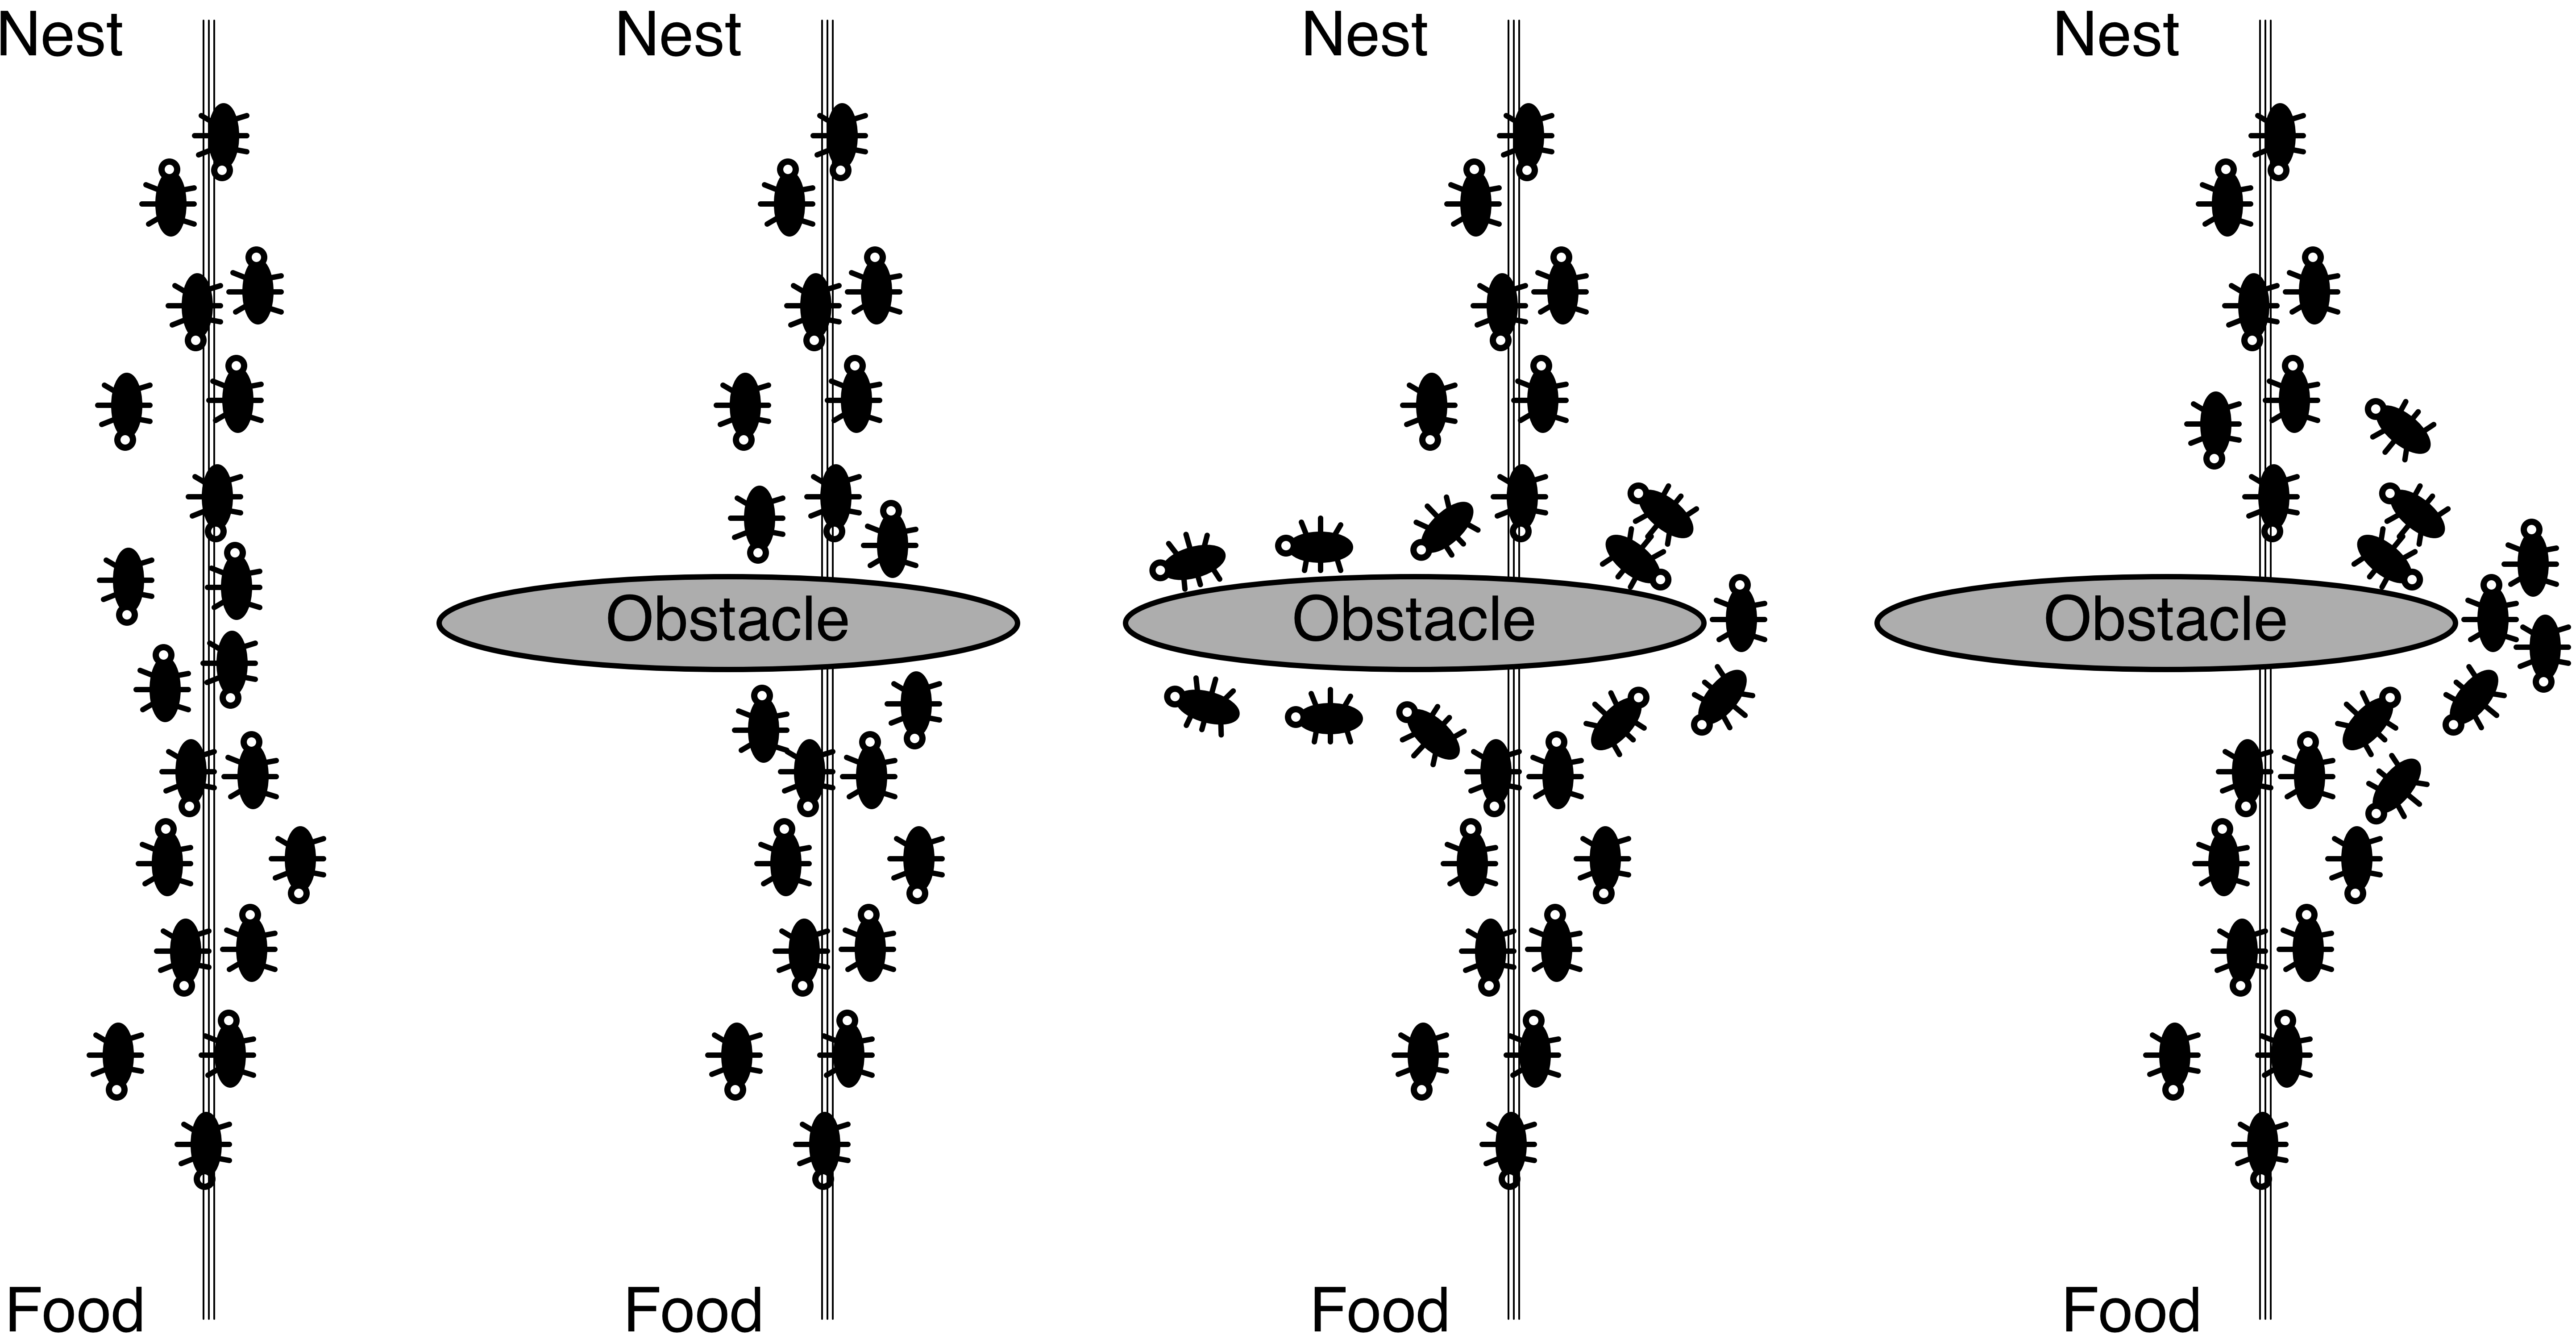
\includegraphics[width=0.85\textwidth]{aco-obstacle.png}
	\caption[The process of ants following a pheromone trail]{The process of ants following a pheromone trail between a food source and their nest affected by an obstacle. Modified from \citet{talbi2009metaheuristics}.}
	\label{fig:aco-obstacle}
\end{figure}

The artificial ants in \gls{aco} are inspired by this behavior and iteratively build a solution by probabilistically choosing the next part based on heuristic, problem-specific information, and, analogous to the real ants, artificial pheromone information. The use of multiple agents also gives the algorithm more robustness and diversification in solving a problem \cite{dorigo2019ant}.

\begin{algorithm}
	\caption{Ant Colony Optimization}
	\label{alg:aco}
	
	\begin{algorithmic}
		\State Initialize pheromone information
		\Repeat
		\For{each ant}
		\State \Call{ConstructSolution}{}
		\EndFor
		\Procedure{UpdatePheromones}{}
		\State \Call{Evaporation}{}
		\State \Call{Reinforcement}{}
		\EndProcedure
		\Until{termination criterion met}
	\end{algorithmic}
\end{algorithm}

The algorithmic implementation is quite straightforward. And since its original use was often adapted for the \gls{tsp}, and this thesis solves that problem as well, the following description is slightly modified to fit it.
\Cref{alg:aco} shows the basic template of the \gls{aco}. First, the pheromone information is initialized uniformly, so that each path is initially equally likely to be chosen. With a total of $n$ cities to visit, the resulting matrix is of dimension $n \times n$, where each entry $\tau_{ij}$ represents the amount of pheromone being present at the edge $(i,j)$.
For every complete cycle, each of $m$ ants probabilistically creates a solution with this pheromone information $\tau_{ij}$ and heuristic information $\eta_{ij}$. Starting from a randomly selected city $i$, the probability to visit the next possible city $j$ from a set $S$ of not yet visited cities is given by 
\begin{equation}
		\label{eq:aco_prob}
		p_{ij} = \frac{\tau_{ij}^\alpha \cdot \eta_{ij}^\beta}{\sum_{h \in S} \tau_{ih}^\alpha \cdot \eta_{ih}^\beta}
\end{equation}
where $\eta_{ij}$ holds the problem specific heuristic value, which is the inverse distance $\eta_{ij} = \frac{1}{d_{ij}}$ between cities $i$ and $j$ in case of the \gls{tsp}. The constants $\alpha, \beta \geq 0$ control the influence of either the stochastic pheromone or the heuristic value. The denominator normalizes the fraction into a probability $0 \leq p_{ij} \leq 1$, with the set of all probabilities from the unvisited cities $S$ effectively creating a probability distribution \cite{talbi2009metaheuristics}.

The pheromone information is then updated based on the generated solutions. First, each pheromone entry is subject to evaporation controlled by a constant value $\rho \in (0,1]$ and defined by the following equation:
\begin{equation}
	\label{eq:aco_evap}
	\forall i,j \in [1,n]: \tau_{ij} \leftarrow (1-\rho) \cdot \tau_{ij}
\end{equation}
In the following reinforcement phase, different strategies can be applied to select how the solutions chosen by the ants influence the pheromone matrix. There are also versions of the \gls{aco} where this procedure is called after each step of the solution construction, or at least after a single ant, but not necessarily after each ant has finished constructing its solution. More common, however, are offline strategies that are called after each ant has finished. One of the simpler implementations in this category is the \enquote{elitist pheromone update}, where the updates of the pheromone matrix are strongly influenced by the global best solution. Another approach is the \enquote{quality-based pheromone update} or \enquote{ant-cycle} \cite{dorigo1996ant}, where each ant $k = 1,2,...,m$ updates the pheromone matrix relative to the length of the solution $L_k$ they found in that iteration, which is further controllable by a parameter $Q \geq 1$. The following two equations define this strategy:
\begin{equation}
	\tau_{ij} \leftarrow \tau_{ij} + \sum_{k=1}^{m} \Delta\tau_{ij}^k 
\end{equation}
\begin{equation}
	\Delta\tau_{ij}^k = \begin{cases}
		\frac{Q}{L_k}, &\text{if edge } (i,j) \text{ is in $k$-th ant tour,} \\
		0, &\text{otherwise}
	\end{cases}
\end{equation}

This loop is repeated until a termination criterion is met. This can be a fixed number of iterations $\text{NC}_{\text{MAX}}$ or until the solution quality stagnates for a certain number of iterations. With the pheromone update implemented as an \enquote{ant-cycle} the time complexity of this algorithm is $O(\text{NC}\cdot n^2 \cdot m)$ \cite{dorigo1996ant}. Based on this algorithm, a large number of variants have been created. One of them is a population-based approach, which is discussed in the following.

\subsubsection{Population-Based Ant Colony Optimization}
The \gls{paco} was first proposed by \citet{guntsch2002population} as a simplification of the \gls{aco}, effectively reducing the operations required to update the pheromone information by quantifying and limiting the values added to the matrix. Their motivation was to speed up the process and reduce the influence of older solutions in order to apply the \gls{paco} to the \gls{dtsp}. 
Instead of storing all updates to the pheromone matrix, the approach keeps track of the solutions that have updated the solution in a queue, called the \textit{population}. Therefore, every solution in this queue is actually present in the matrix and vice versa. To limit the influence of old solutions, the population size is set to a value $k$. When the queue is full after $k$ iterations, several actions are possible in iteration $k+1$, with the most obvious being to implement a FIFO (first in, first out) behavior, discarding the oldest solution. This also eliminates the need for evaporation. The rest of the algorithm is analogous to the \gls{aco} presented earlier. The matrix is initialized with a constant amount $\tau_{\text{init}}$. The pheromone update is done by the ant with the iteration best solution. With a weight $w_e \in [0,1]$ controlling the amount of pheromone deposited and a maximum set to $\tau_{\text{max}}$, the amount of pheromone added is defined by $(1-w_e) \cdot (\tau_{\text{max}} - \tau_{\text{init}})/k$.
This reduces the number of pheromone updates per generation, for a \gls{tsp} instance of $n$ cities, from $n^2$ operations to at most $2n$ operations \cite{guntsch2002population}.

\begin{figure}
	\hfill
	\begin{subfigure}{.3\textwidth}
		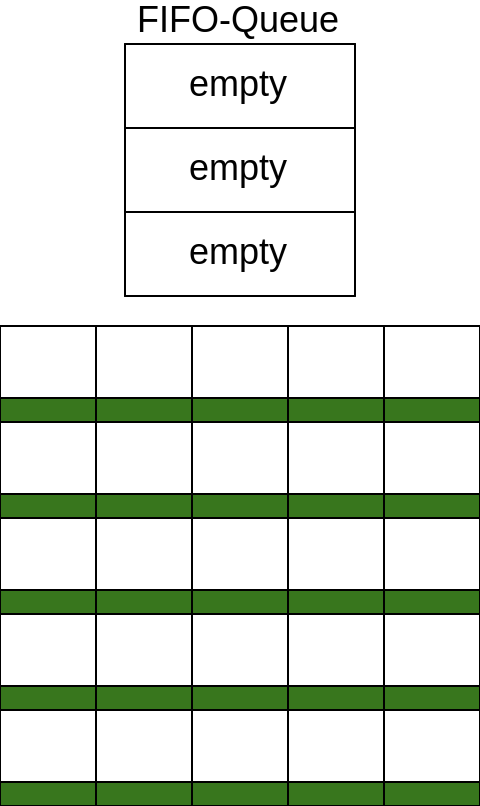
\includegraphics[width=\textwidth]{paco-1.svg}
		\caption{Matrix at $i=0$}
		\label{fig:paco1}
	\end{subfigure}
	\hfill
	\begin{subfigure}{.3\textwidth}
		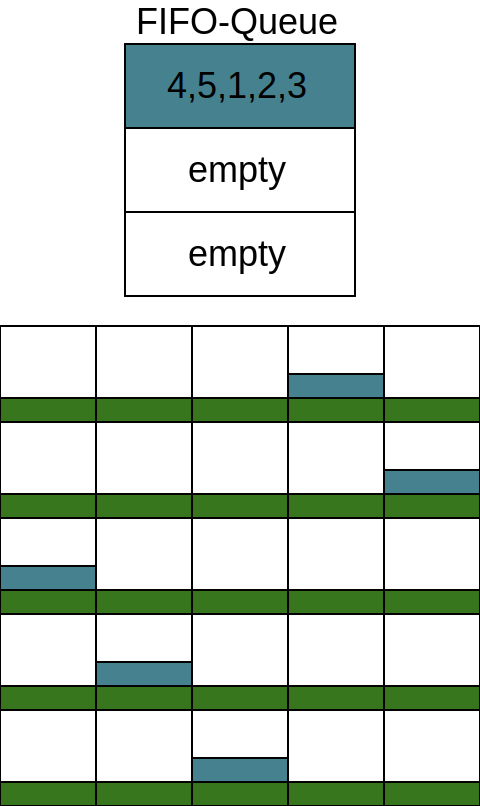
\includegraphics[width=\textwidth]{paco-2.svg}
		\caption{Matrix at $i=1$}
		\label{fig:paco2}
	\end{subfigure}
	\hfill
	\begin{subfigure}{.3\textwidth}
		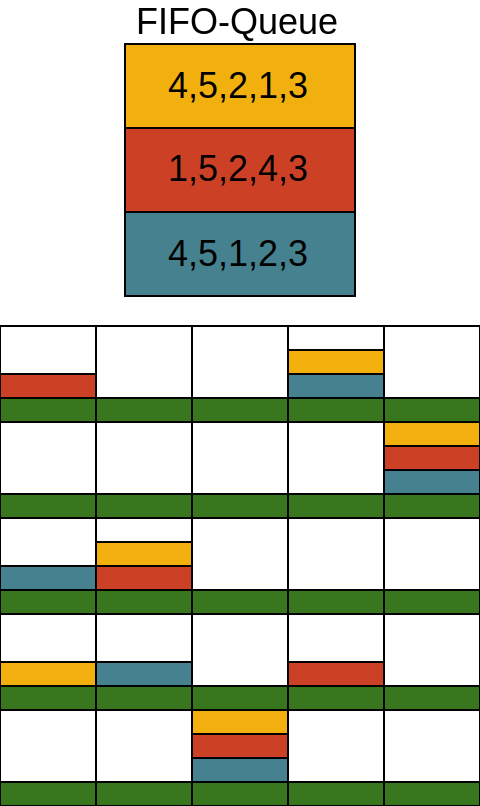
\includegraphics[width=\textwidth]{paco-3.svg}
		\caption{Matrix at $i=3$}
		\label{fig:paco3}
	\end{subfigure}
	\caption[Example of a \gls{paco} matrix being updated over multiple iterations]{Example of a \gls{paco} matrix being updated over multiple iterations for a solution population size of $k=3$. The rows represent the location of the solution ranging from $1$ to $n$, while the columns depict the option chosen (e.g., a city node for the \gls{tsp}).}
	\label{fig:paco}
\end{figure}

\Cref{fig:paco} shows an example of a pheromone matrix with a solution population of $k=3$ being updated over the course of three iterations for a problem of size $n$. In \cref{fig:paco1}, the population is empty and the matrix is initialized with $\tau_{\text{init}}$, visualized by the green bars. The best solution of the first iteration has the city referenced at position 4 as its start, continuing with position 5, and so on. This update is visualized by blue colored bars. Eventually, after two more iterations (\cref{fig:paco3}), the population queue is full. In a next iteration, the solution visualized in blue would leave the matrix and a new one would be placed at the top of the queue.

\subsection{Particle Swarm Optimization}

The \gls{pso} method was introduced by \citet{kennedy1995particle} as a \enquote{concept for optimization of nonlinear functions} by simulating swarms of birds or fish in their search for food. The individuals, referred to as \textit{particles}, iteratively explore a given problem space of dimension $d$. Therefore, each of the $N$ particles in a swarm represents a candidate solution to the problem, evaluated by an objective fitness function $f: \mathbb{R}^d \to \mathbb{R}$. Furthermore, each particle $i$ is defined by three vectors and two values:
\begin{itemize}
	\item the current position $\vec{x_i} \in \mathbb{R}^d$ 
	\item the current velocity $\vec{v_i} \in \mathbb{R}^d$ 
	\item the best solution found so far $\vec{p_i} \in \mathbb{R}^d$
	\item the fitness values $f(\vec{x_i})$ and $f(\vec{p_i})$
\end{itemize}

To let the particles influence each other, a neighborhood rule must be defined. The most straightforward way is the global best method (\textbf{gbest}), where all particles influence each other without restrictions. Another, potentially more complex, strategy for letting the particles exchange information is the local best method (\textbf{lbest}). In this method, particles interact based on a given topology, such as a ring, where only direct neighbors exchange information. Thus, regardless of the strategy chosen, each neighborhood $k$ has a leader with the best solution $\vec{g_k}$ \cite{talbi2009metaheuristics}. Putting both aspects together, the particles update their velocity based on personal success (\textit{cognitive aspect}) and neighborhood success (\textit{social aspect}) \cite{janson2003hierarchical}. 

\begin{algorithm}
	\caption{Particle Swarm Optimization}
	\label{alg:pso}
	\begin{algorithmic}
		\State Initialize swarm
		\Repeat
		\ForAll{particles $i \in [1, N]$}
		\State \Call{UpdateVelocities}{}
		\State \Call{UpdatePosition}{}
		\If{$f(\vec{x_i}) < f(\vec{p_i})$} {$\vec{p_i} = \vec{x_i}$}
		\If{$f(\vec{x_i}) < f(\vec{g_k})$} {$\vec{g_k} = \vec{x_i}$}\EndIf \EndIf
		\EndFor
		\Until{termination criterion met}
	\end{algorithmic}
\end{algorithm}

\Cref{alg:pso} shows a high-level description of the \gls{pso} procedures. Typically, the swarm is randomly initialized, with each particle assigned a velocity and a position in the search space. The resulting solutions are set as $\vec{p_i}$ and, for each particle's neighborhood $k$, the leader solution $\vec{g_k}$ is determined. After the initialization, each particle $i$ updates its velocity $\vec{v_i}$ per iteration $t$ according to the following equation:
\begin{equation}
	\vec{v_i}(t+1) = w \cdot \vec{v_i}(t) + c_1 \cdot r_1 \cdot (\vec{p_i} - \vec{x_i}(t)) + c_2 \cdot r_2 \cdot (\vec{g_k} - \vec{x_i}(t))
\end{equation}

with an inertia weight $w > 0$ that controls the influence of particle velocity. The parameters $c_1, c_2 > 0$ define the influence of the personal best $\vec{p_i}$ and the neighborhood best solution $\vec{g_k}$, respectively and are additionally subject to a random factor due to values $r_1, r_2$ drawn from a uniform distribution of $[0,1]$. Afterwards, the particle's position is updated: 
\begin{equation}
	\vec{x_i}(t+1) = \vec{x_i}(t) + \vec{v_i}(t+1)
\end{equation}  
Lastly, the best solutions are potentially updated if they are better than the current ones. To ensure convergence of the swarm, many implementations also limit the velocity to a certain value or reduce the inertia weight over time.
This whole process is visualized in \cref{fig:pso-vector}, which shows a particle $i$ being updated according to all three possible influences. 

  \begin{figure}
	\centering
	\begin{tikzpicture}[thick,>={Triangle[angle=30:4pt 4]}]
		\coordinate[label={[xshift=-10]left:{$x_i(t)$}}] (O) at (0,0);
		\coordinate[label=0:{$p_i$}] (A) at (1,2);
		\coordinate[label=0:{$g_k$}] (B) at (5,1);
		\coordinate (C) at (2,-2);
		\coordinate (C2) at (1.9,-2.1);
		\coordinate[label={[xshift=+10pt]right:{$x_i(t+1)$}}] (S) at ($0.5*(A)+0.3*(B)+0.8*(C)$);
		\coordinate (S1) at ($(O)+0.8*(C)$);
		\coordinate (S2) at ($(S1)+0.5*(A)$);
		\coordinate (S3) at ($(S2)+0.3*(B)$);
		
		\node[fill=gray,circle,left,radius=5pt] at (O) {};
		\node[fill=gray,circle,right,radius=5pt] at (S) {};
		
		\draw[->] (O) -- (A) node[midway,auto] {$p_i - x_i(t)$} ;
		\draw[->] (O) -- (B) node[midway,above] {$g_k - x_i(t)$} ;
		\draw[->] (O)+(-0.1,-0.1) -- (C2) node[midway,below left] {$v_i(t)$} ;
		\draw[->, dashed] (O) -- (S1) ;
		\draw[->, dashed] (S1) -- (S2) ;
		\draw[->, dashed] (S2) -- (S) ;
	\end{tikzpicture}
	\caption[The vector summation of a \gls{pso} particle]{The vector summation of a \gls{pso} particle $i$ during velocity and position update.}
	\label{fig:pso-vector}
\end{figure}

Research has been performed to understand how the algorithm behaves and how to vary the algorithm. In particular, the choice of neighborhood topology has a significant impact on performance. The \textbf{gbest} method seems to perform better on unimodal problems, where there is one clear function optimum, while the \textbf{lbest} method gives better performance on multimodal problems with many optimal function values \cite{janson2003hierarchical}. 

\label{chap:hpso}
One such variant is the \gls{hpso} proposed by \citet{janson2003hierarchical}, which uses a hierarchical tree topology (indicating solution quality) to define a neighborhood. The resulting (almost) regular tree has a total number of $m$ nodes over a height $h$, where each parent node has at most $d$ children. The particles are represented by the nodes of the tree, and, therefore, the neighborhood of each particle $i$ is defined only by its direct parent $j$ in this hierarchy, so $\vec{g_i} = \vec{p_j}$. 
The updating of velocity and position remain the same as in the standard approach, but the comparison and eventual update of the neighborhood best solution $\vec{g_k}$ can be seen as a tree restructuring process. If a child node $i$ happens to find a better solution than its parent node $j$, so $f(\vec{p_i}) < f(\vec{p_j})$, they swap their position in the hierarchy. This process is performed top-down, breadth-first, resulting in worse solutions may moving down several levels in an iteration, but good solutions moving up at most one level. The global best solution can then be found at the root position after a maximum of $h$ iterations.

Another variant is called \gls{sso}, which is a discrete version of the \gls{pso}, capable of solving combinatorial problems such as the \textit{MMRAP} (multi-level, multi-state redundancy allocation problem), as proposed by \citet{yeh2009two}. The solution of the particle is no longer represented by the position and the velocity in the multidimensional problem space, but is instead encoded as a finite-length string and an additional fitness value. The update mechanism has also been simplified by probabilistically selecting the next position string based on a random number that may lie in multiple tunable intervals \cite{yeh2012simplified}. These intervals are the probabilities for the personal best solution $p_{\text{pbest}}$, the personal previous solution $p_{\text{pprev}} $ and the global best solution $p_{\text{gbest}}$. The resulting solution vector $\mathbf{s}^{t+1}_j$ for particle $j$ at iteration $t+1$ is therefore built according to
\begin{equation}
	\label{eq:sso_rule}
	s_{ij}^{t+1} = \begin{cases}
		s^t_{ij} & \text{ with propability } p_{\text{pprev}}, \\
		p^t_{ij} & \text{ with propability } p_{\text{pbest}}, \\
		g^t_{i} &\text{ with propability } p_{\text{gbest}}, \\
		v & \text{ with propability } p_{r}
	\end{cases}
\end{equation}
with $s_{ij}$ being the $i$-th solution component of particle $j$ and $v \in V$ being a value from a set of all feasible values chosen with probability $p_r$ \cite{lin2015simple}. 


\subsection{SPPBO Framework and H-SPPBO Algorithm}

\subsubsection{Simple Probabilistic Population-Based Optimization}

The \gls{sppbo} is a metaheuristic scheme that combines generalized aspects of population based approaches, such as \gls{pso} and \gls{sso}, and strategies that effectively generate probability distributions, such as \gls{aco} and \gls{paco}. As discussed by \citet{lin2015simple}, the framework can be used to classify and virtually recreate many of these metaheuristics for solving discrete combinatorial problems by using two simple operations: 
\begin{itemize}
	\item \textit{SELECT+COPY}: Selecting a solution from the population and copying (parts of) this solution when certain conditions apply.
	\item \textit{RANDOM}: Random selection of a value from the set of possible values.
\end{itemize}
These operations can be used to create multiple variants of an \gls{sppbo} algorithm, as well as de facto implementations of \gls{paco} and \gls{sso}. However, they all share the same schematic foundation. First, a distinction must be made between populations and \glspl{sce}. Reminiscent of an ant (\gls{aco}) or a particle (\gls{paco}),  a set of \glspl{sce} $\mathcal{A}$ create the solutions by applying probabilistic rules $\text{Prob}_V$ and, optionally, some form of heuristic information $\eta$. These solutions may then enter a set of populations $\mathcal{P}$ (cmp. \gls{paco}). $V$ denotes the set of possible values $v_i \in V$ that may appear in a solution vector $\textbf{s} \in V^n$ of length $n$. 
The high-level structure of these \gls{sppbo} metaheuristics is shown in \Cref{alg:sppbo}.

\begin{algorithm}
	\caption{SPPBO}
	\label{alg:sppbo}
	\begin{algorithmic}
		\State Initialize random solutions
		\Repeat
		\ForAll{SCE $A \in \mathcal{A}$}
			\State \Call{Create}{$A$}
		\EndFor
		\ForAll{population $P \in \mathcal{P}$}
			\State \Call{Update}{$P$}
		\EndFor
		\Until{termination criterion met}
	\end{algorithmic}
\end{algorithm}

After the populations are initialized with random solutions, each \gls{sce} creates one solution, resulting in $k_{\text{new}} = \abs{\mathcal{A}}$ new solutions per iteration. The underlying probability distribution is affected by three aspects:
\begin{itemize}
	\item The populations in the \gls{sce}'s neighborhood ($\text{Range}_P \subseteq \mathcal{A}$),\\realizing the \textit{SELECT+COPY} operation.
	\item The set of feasible values $V$, realizing the \textit{RANDOM} operation.
	\item The problem-specific heuristic information $\eta$.
\end{itemize}
Additionally, the influence of the \textit{SELECT+COPY} and \textit{RANDOM} operations on the population can be further controlled by the weights $w_p$ and $w_r$. The populations are then updated based on a set of rules specific to the implementation. For example, in a version of \gls{sppbo} with only one global best population, the update procedure may insert the iteration best solution and save a total of $k$ iterations \cite{lin2015simple}.

\subsubsection{Hierarchical Simple Probabilistic Population-Based Optimization}
\label{chap:hsppbo}

Building on the schematic foundation of the \gls{sppbo}, the \gls{hsppbo} was designed using its principles. Combining the hierarchical aspect of \gls{hpso} with a probabilistic solution creating approach similar to \gls{sso}, while maintaining a population of solutions such as \gls{paco}, the goal of this algorithm, as stated by \citet{kupfer2021hierarchical}, was to not only to solve the \gls{dtsp}, but also to detect these dynamic changes and react accordingly. 

Similar to the descriptions of \gls{sppbo}, there is a set $\mathcal{A}$ of \glspl{sce} and a set of populations $\mathcal{P}$. The important difference here is that these populations $P \in \mathcal{P}$ each belong to a \gls{sce} $A \in \mathcal{A}$, which is described by a function $P\in \text{range}(A) \subseteq \mathcal{P}$, that dynamically adapts to changing neighborhood relations. To take advantage of these parent-children relationships in the population, the hierarchical aspect is implemented similarly to \gls{hpso} (see \cref{chap:hpso}). The \glspl{sce} are organized in an $m$-ary tree\footnote{A tree structure in which every node has at most $m$ children, with no restriction on height. For example, a value of $m=2$ would result in a binary tree.}, where each \enquote{child SCE} is influenced by its $\text{parent}(A)$, and a \enquote{root SCE} $A*$, defined as its own parent ($\text{parent}(A*) = A*$). This hierarchy allows for a clear definition of the following populations $P\in \mathcal{P}$ for each \gls{sce} $A$:
\begin{itemize}
	\item the personal previous solution $P^{A}_{\text{persprev}}$
	\item the personal best solution $P^{A}_{\text{persbest}}$
	\item the parent best solution $P^{A}_{\text{parentbest}}$
\end{itemize}
Each population contains exactly one solution vector $\mathbf{s} \in V^n$ (e.g., for a \gls{tsp} instance of size $n$) from the set of all feasible values $V$. Note also that due to the tree structure $P^{A}_{\text{parentbest}} = P^{\text{parent}(A)}_{\text{persbest}}$. Each of these populations has a corresponding weight $w_{\text{persprev}}, w_{\text{persbest}}, w_{\text{parentbest}} \geq 0$ to control their respective influence. 
Now, to create a solution $\mathbf{s}$, the probabilistic rule is very similar to the one used by \gls{sso} seen in Eq. \eqref{eq:sso_rule}, with $p_{\text{gbest}}$ referring to the best solution of the parent and a distinct random influence $p_r$ through a random weight $w_\text{rand}$.

The following description of the algorithm and the equations are adapted to fit the \gls{tsp}, since the \gls{hsppbo} was originally created to solve the \gls{tsp} and its dynamic variant. A modification to solve other combinatorial problems, such as the \gls{qap}, would be straightforward, but is not discussed in this thesis.

\begin{algorithm}
	\caption{H-SPPBO}
	\label{alg:hsppbo}
	\begin{algorithmic}
		\State Initialize the \gls{sce} tree
		\State Initialize \glspl{sce} with random populations $P^A_{\text{persprev}}$,$P^A_{\text{persbest}}$
		\Repeat
		\ForAll{SCE $A \in \mathcal{A}$}
		\State \Call{CreateSolution}{$A$} \Comment{using \eqref{eq:hsppbo_tau} and \eqref{eq:hsppbo_prob}}
		\State \Call{UpdatePopulations}{$P^A_{\text{persprev}}, P^A_{\text{persbest}}$}
		\EndFor
		\State $\text{swapNum} = 0$
		\ForAll{SCE $A \in \mathcal{A}_{\text{tree}}$ }
		\If{$f(\mathbf{s}^A_{\text{persbest}}) < f(\mathbf{s}^{\text{parent($A$)}}_{\text{persbest}}) $}
		\State \Call{Swap}{$A$, $\text{parent}(A)$}
		\State $\text{swapNum} \gets  \text{swapNum} + 1$
		\EndIf
		\EndFor
		\If{$\text{swapNum} > [\theta \cdot \abs{\mathcal{A}}]$ $\mathbf{and}$ no change in $L_\text{pause}$ previous iterations}
		\State \Call{ChangeHandlingProcedure}{$H$}
		\EndIf
		\Until{termination criterion met}
	\end{algorithmic}
\end{algorithm}

\Cref{alg:hsppbo} shows the process for solving a dynamic problem. It is similar to the template given for \gls{sppbo} (see \Cref{alg:sppbo}), with a solution creation and a population update phase. However, since the populations are directly related to the \glspl{sce}, the update phase is performed in the same loop.
First, the \gls{sce} tree is initialized with a number of $\abs{\mathcal{A}}$ randomly set \glspl{sce} and their two solution populations.
Then, at each iteration, every \gls{sce} creates one solution using the following procedure: Start with a set of all unvisited nodes $U \subseteq V$ and set a random starting node $i$. Now, calculate the following term $\tau_{ik}$ for all possible nodes $k \in U$ by
\begin{equation}
	\label{eq:hsppbo_tau}
	\tau_{ik}(A) = \left(  w_{\text{rand}} + \sum_{P\in \text{range}(A)} w_P \cdot s_{ik}(P)  \right)^\alpha \cdot \eta^\beta_{ik}
\end{equation}
\begin{equation*}
	s_{ik}(P) = \begin{cases}
		1 & \text{if $(i,k) \subset \mathbf{s}_P$},\\
		0 & \text{otherwise}
	\end{cases}
\end{equation*}
with $\text{range}(A)$ giving all three populations assigned to the \gls{sce} as mentioned above, and a heuristic component $\eta_{ik}$ set as the inverse distance $1 / d_{ik}$ between nodes $i$ and $k$ which is typical for the \gls{tsp}. This $\tau$-term effectively accumulates all the different weights by using $s_{ik}(P)$ as an activation function to check whether the current, possible edge $(i,k)$ has been previously visited by the \gls{sce} ($P^{A}_{\text{persprev}}, P^{A}_{\text{persbest}}$) or its parent ($P^{A}_{\text{parentbest}}$), i.e., formally, if the ordered set $(i,k)$ is a subset of the solution vector $\mathbf{s}_P$ of the population $P$. The following example is given for clarification:
\begin{example}[A subset of an ordered set]
	\label{ex:subset}
Using the \gls{tsp} instance from Fig.\ref{fig:ExampleTSP}, a previous solution of a \gls{sce} might be $\mathbf{s}_\text{persprev} = (4,2,3,1) \in V^4$. Then, $(4,2)$ would be an ordered subset of that solution, $s_{4,2}(P_\text{persprev}) = 1$.
\end{example}
As in the \gls{aco} metaheuristic, $\alpha, \beta \geq 0$ are parameters to control the stochastic and heuristic influence, respectively. 
The probability of visiting node $j$ after node $i$ can now be defined by
\begin{equation}
	\label{eq:hsppbo_prob}
	p_{ij}(A) = \frac{\tau_{ij}(A)}{\sum_{k \in U} \tau_{ik}(A)}
\end{equation}
where the denominator is used to normalize this term to a probability distribution over all unvisited nodes $U$. Finally, a node $j$ is randomly drawn from this distribution, added to the solution vector $\mathbf{s}$ and removed from the unvisited set $U \gets {j}\setminus U$. With this new node being the next current node, the process is repeated until the set of unvisited nodes is exhausted. And eventually, the populations are updated.

With new solutions calculated, the hierarchy is now subject to change. The \gls{sce} tree is iterated in a top-down, breadth-first manner ($\mathcal{A}_\text{tree}$), and each \gls{sce} compares its personal best solution with its parent by using an evaluation function $f : V^n \rightarrow \mathbb{R}_{0}^{+}$, which in case of the \gls{tsp}, is just the length of the tour $L$. If the child has a better solution quality than its parent, so $f(\mathbf{s}^A_{\text{persbest}}) < f(\mathbf{s}^{\text{parent($A$)}}_{\text{persbest}})$, they swap their places. Thus, making the $\text{range}$ function dynamically changing by also swapping the $P^{A}_{\text{parentbest}}$ population. An example of this swap operation is shown in \cref{fig:ternary-tree}. By using this top-down approach, comparatively worse solutions can descend all the way to the lowest level in one iteration, while good solutions may only be able to move up one tier. Nevertheless, if no new personal best solutions have been found in at least as many iterations as the number of levels of the tree $h$, the global best solution is able to move to the root of the \gls{sce} tree.

Since the \gls{hsppbo} should also detect and react to dynamic changes in the \gls{tsp} instance, the last part of the algorithm is executed when a certain threshold of rearrangements in the \gls{sce} tree is exceeded. Specifically, the number of swaps from the previous part is being compared to a percentage of \glspl{sce} in the tree $\abs{\mathcal{A}}$. This is controlled by a constant $\theta \in [0,1]$, with a higher value reducing the detection sensitivity and an extreme of $\theta = 1$ requiring a complete rearrangement of the tree to render the condition true. However, this condition may be met without the problem instance actually changing, leading to false detections. Regardless, when the change handling procedure is triggered by \enquote{enough} change, one of two $H$ mechanisms is executed to alter the \glspl{sce}, ideally aiding in creating better solutions to this (possibly) modified problem. The strategies are the following:
\begin{itemize}
	\item $H_\text{full}$ resets the $P^{A}_{\text{persbest}}$ population for all \glspl{sce} $A \in \mathcal{A}$ to a random solution.
	\item $H_\text{partial}$ resets only the $P^{A}_{\text{persbest}}$ population of the \glspl{sce} starting from the third level down, leaving the the root and its children unaltered.
\end{itemize}

While $H_\text{full}$ can be understood as a complete reset of the algorithm, $H_\text{partial}$ tries to apply some of the best \enquote{knowledge} to solve this changed problem (exploitation), while the lower performing \glspl{sce} may instead concentrate on finding new solutions (exploration). Additionally, due to the potentially major rearrangements in the tree as a result to these change handling procedures being executed, the parameter $L_\text{pause} > 0$ acts as a guardrail to prevent the procedure from virtually triggering itself, providing the hierarchy a few iterations to settle \cite{kupfer2021hierarchical}.

\begin{figure}
\centering
\resizebox{0.9\textwidth}{!}{
		\begin{forest}
			baseline,for tree={
				anchor=center,
				grow=south,
				circle, draw, inner sep=2pt, minimum size=1.4em,
				s sep=(3-level)*1mm
			}
			[a, baseline, {draw=red},
			[b, 
			[e][f][g]
			][c, {draw=blue},
			[h][i][j]
			][d
			[k][l][m]
			]
			]
		\end{forest}
	\quad
		\begin{forest}
			baseline,for tree={
				anchor=center,
				grow=south,
				circle, draw, inner sep=2pt, minimum size=1.4em,
				s sep=(3-level)*1mm
			}
			[c, baseline, {draw=blue},
			[b
			[e][f][g]
			][a, {draw=red},
			[h][i][j]
			][d
			[k][l][m]
			]
			]
		\end{forest}}
	\caption[Example of a ternary SCE tree showing a swap operation]{Example of a ternary SCE tree ($m = 3$) with height $h = 3$ showing the \textsc{Swap(a,c)} operation before (left) and after (right) the execution. Modified from \citet{kupfer2021hierarchical}.}
	\label{fig:ternary-tree}
\end{figure}



\section{Parameter Optimization for Metaheuristics}

\subsection{Overview}

Every metaheuristic has at least a few parameters to control its behavior. This is not only a byproduct of ambivalent algorithm design, but more often to allow more flexibility in solving multiple problems with different qualities. For example, looking at the \gls{aco} (see \ref{chap:aco}), there is the number of ants $m$, the trail persistance rate $\rho$, the initial amount of pheromone $\tau_0$, the relative quantity of pheromone added $Q$, and the importance of stochastic aspects $\alpha$ and heuristic information $\beta$. And as mentioned in \cref{chap:paramopt}, the performance of these algorithms depends heavily on optimal parameters, without a priori knowledge of which settings to choose.

\begin{figure}[h]
	\centering
	
\includegraphics[width=0.9\textwidth]{metaheuristic_parameter_classification.svg}
	\caption[Taxonomy of parameter optimization]{Taxonomy of parameter optimization. Modified from \citet{eiben1999parameter}.}
	\label{fig:paramtax}
\end{figure}

This thesis applies methods from machine learning research to address this challenge. Therefore, the following review of parameter optimization methods classifies this technique and identifies other possible strategies. \Cref{fig:paramtax} shows a taxonomy of parameter optimization methods from \citet{eiben1999parameter}, with additions from \citet{talbi2009metaheuristics} and \citet{stutzle2012parameter}. There are two main differences: \enquote{Parameter Tuning} (offline initialization) tries to find good parameter settings before the algorithm is even applied, and these settings remain fixed afterwards. \enquote{Parameter Control} (online initialization) modifies the parameters while the algorithm is running, allowing for potentially better adaptation to the problem.

\subsubsection{Parameter Control}

Parameter control methods can be advantageous because they can adapt to the problem instance over time. They can also be used to encourage certain search phases of the algorithm, increasing either the exploratory or the exploitative behavior after a certain time. Several ways of implementing such online parameter initialization methods have been proposed. \textit{Dynamic} strategies alter the values according to a specific deterministic rule, while also allowing for minor random influences on the parameters. \textit{Adaptive} optimization, on the other hand, takes additional feedback from the metaheuristic algorithm to control the weight for its change, but still relies on predefined functions for this. Lastly, \textit{self-adaptive} parameter control implements the parameter change into the metaheuristic algorithm itself, making it part of its search space and thus the solution.

\subsubsection{Parameter Tuning}
\label{chap:tuning}

The simplest method of parameter tuning is a manual trial-and-error approach. By tuning one parameter at a time, each parameter is evaluated on its own, but without considering the interactions between them. This also becomes a very time consuming and error prone process as the parameter space grows.
Two methods address these issues with offline tuning. The first is a \gls{doe} approach to determine the minimum required scope of the experiments needed and to arrange the test points within the parameter space based on an optimality criterion. The result of these experiments should reveal a good set of parameters, with the possibility of further statistical significance tests.  
The other method uses meta-optimization, which is an algorithmic layer on top of the metaheuristic to find optimal parameter values. This can be either a metaheuristic algorithm (like \gls{pso}) or a machine learning based approach, which is discussed in the following subsection.


\subsection{Hyperparameter Optimization}
\label{chap:hyperopt}

In \gls{ml} applications hyperparameters are used to configure a \gls{ml} model. Similar to parameters in metaheuristics, tuned hyperparameters can greatly improve the performance of a \gls{ml} model over the default settings. In particular, state-of-the-art deep learning techniques, which have a large number of tunable parameters, can only be properly utilized if the hyperparameters are specifically tuned for their problem.

Traditionally, simple gradient descend-based approaches are often used for optimization problems. In its simplest form, the objective function $f(x)$ is to be minimized by $\min_{x \in \mathbb{R}} f(x)$, with a region of feasible values $D = \left\lbrace { x \in X | g_i(x) \leq 0, h_j(x) = 0}\right\rbrace $, and possible range and equality constraints $g_i(x), h_j(x)$ from a set of all values $X$. Following the negative gradient direction, a global optimum could be obtained for convex functions \cite{yang2020hyperparameter}. 
However, \gls{ml} models pose some challenges to these established techniques:
\begin{enumerate}
	\item The underlying objective function of a \gls{ml} model is usually not convex nor differentiable. Therefore, methods like gradient descend often result in local optima.
	\item The hyperparameters of \gls{ml} models are in the domain of continuous (real-valued),  discrete (integer-valued), binary, categorical and even conditional values. This results in a complex configuration space with sometimes non-obvious value ranges.
	\item Objective function evaluations can be very expensive, which necessitates methods for quicker, more efficient sampling. 
\end{enumerate}

In parallel with research on optimal parameters for metaheuristics (see \ref{chap:paramopt}), the manual tuning of hyperparameters in \gls{ml} applications began to become impractical in the face of more complex and feature-rich models. Therefore, interest in the automated tuning of hyperparameters, called \gls{hpo}, began in the 1990s. With important use cases being the reduction of human effort, the improved performance of these algorithms and, especially in scientific research, to help reproducibility, much progress has been made since the above-mentioned gradient descent-based methods were first applied  \cite{feurer2019hyperparameter}. 

The \gls{hpo} problem statement can be formulated as follows \cite{feurer2019hyperparameter}:
Let $\mathcal{A}$ be a \gls{ml} algorithm with $N$ hyperparameters, where $\Lambda_n$ denotes the $n$-th hyperparameter. The complete hyperparameter configuration space can then be defined as $\mathbf{\Lambda} = \Lambda_1 \times \Lambda_2 \times ... \times \Lambda_N$, with a vector of a possible hyperparameter configuration $\mathbf{\lambda} \in \mathbf{\Lambda}$. Thus, a \gls{ml} algorithm initialized with hyperparameters $\mathbf{\lambda}$ is denoted by $\mathcal{A}_\mathbf{\lambda}$.
Based on this, the process of \gls{hpo} consists of four main components: 1) an estimator (most often a regressor, but a classifier is also possible), 2) a search space $\mathbf{\Lambda}$, 3) a method to select configurations from the search space, and 4) a validation protocol $\mathcal{V}$ and its loss function $\mathcal{L}$ to evaluate the performance of the configuration (e.g., error rate or root mean squared error). 
The goal is then to find the optimal hyperparameter set $\mathbf{\lambda^*}$ on a given data set $\mathcal{D}$ divided into training data $D_\text{train}$ and validation data $D_\text{valid}$ that minimizes the expected value $\mathbb{E}$ of the validation protocol:
\begin{equation}
	\label{eq:hpo}
	\mathbf{\lambda^*} = \operatorname*{argmin}_{\mathbf{\lambda} \in \mathbf{\Lambda}} \mathbb{E}_{(D_\text{train}, D_\text{valid}) \sim \mathcal{D}} \left[ \mathcal{V}(\mathcal{L}, \mathcal{A}_\mathbf{\lambda}, D_\text{train}, D_\text{valid}) \right] 
\end{equation}

Almost all of this also applies to the parameter optimization for metaheuristic algorithms. Here, the loss function $\mathcal{L}$ is often closely related to the objective function itself, e.g., the resulting tour length in solutions to the \gls{tsp}. Therefore, \gls{hpo} for metaheuristics has no need for any supervised data sets or ground truths. Applied to metaheuristics solving the \gls{tsp}, with the solution quality function $f(\mathbf{s})$ from \cref{eq:solution_quality}, the \gls{hpo} goal from \cref{eq:hpo} can be defined as follows:
\begin{equation}
	\label{eq:hpo-meta}
	\mathbf{\lambda^*} = \operatorname*{argmin}_{\mathbf{\lambda} \in \mathbf{\Lambda}} \mathbb{E} \left[ \mathcal{V}(f, \mathcal{A}_\mathbf{\lambda}) \right] 
\end{equation}
with $\mathcal{A}_\mathbf{\lambda}$ now being the metaheuristic algorithm initialized with parameters $\mathbf{\lambda}$. To simplify all further explanations, let the objective function $f: \mathcal{\mathbf{\Lambda}} \to \mathbb{R}$ be defined directly by its parameter space $\mathcal{\mathbf{\Lambda}}$, which is mapped into the real solution quality space $\mathbb{R}$.

There are several ways to solve the above mentioned problem statements. A common distinction between these methods is their use of the objective function and its loss landscape. A \gls{hpo} algorithm can either treat this as a black-box function, using full evaluations of the objective function to model its behavior, or it can approach the problem with so-called \enquote{multi-fidelity optimization}, where the model is too complex and computationally expensive to use for evaluation and a cheap (possibly noisy) proxy is used instead \cite{feurer2019hyperparameter}. Another important distinction, especially in the area of black-box \gls{hpo}, is whether or not to use a statistical model, .i.e an estimator. Model-free techniques rely solely on function evaluation and factual improvement for their optimization process, without using any prior knowledge to sample the search space. Model-based methods, however, employ a more sophisticated strategy, often implemented using so-called \gls{bo}, which is explained in the next subsection. Other strategies for \gls{hpo} involve evolutionary algorithms or population-based methods, such as \gls{pso} \cite{yang2020hyperparameter}. Although, this approach of using metaheuristics to tune a metaheuristic is similar to the process proposed by \cite{talbi2009metaheuristics} (see \cref{chap:tuning}), it is not used in later stages of the thesis, due to its conflicting nature in the context of parameter optimization applied to a complex metaheuristic such as \gls{hsppbo}.

The following subsections give four examples of black-box \gls{hpo}, with one using model-free and the remaining using model-based, \gls{bo} techniques. All of these methods were also used for the experiments discussed in later sections of this thesis.

\subsection{Grid Search and Random Search}

A very simple and straightforward approach to \gls{hpo} is \gls{gs}. With its basic functionality similar to brute-force methods, it evaluates all possible combinations of hyperparameter values. \gls{gs} only requires finite sets of value ranges to be defined for each hyperparameter, similar to $\Lambda$. It then iterates over the entire search space by creating the Cartesian product of these sets. This approach is easily interpretable and repeatable, while also being trivially implemented and parallelized \cite{bergstra2012random}. However, each new parameter causes the Cartesian product to grow exponentially, so \gls{gs} suffers greatly from the \enquote{curse of dimensionality}. Another problem is its inability to explore promising value ranges on its own. Since these must be predefined, a user would have to manually adjust these ranges before each run \cite{yang2020hyperparameter}.

\gls{rs} was proposed to overcome the limitations of \gls{gs} by sampling the hyperparameters from a probability distribution over the configuration space $F(\mathbf{\Lambda})$, eliminating the need to try all possible combinations \cite{bergstra2012random}. In most cases, this probability distribution is simply uniform for all hyperparameters, but certain applications may warrant for a higher density in some regions of a hyperparameter. \Cref{alg:randomsearch} presents the pseudo-code for the \gls{rs} algorithm. It basically compares each new function evaluation $f(\mathbf{\lambda_{\text{new}}})$ on a randomly sampled parameter $\mathbf{\lambda_{\text{new}}}$. The termination criterion is usually implemented as a fixed budget of function evaluations $B$, thus giving each of $N$ hyperparameters $B$ different evaluations, as opposed to $B^{1/N}$ with \gls{gs} (would it also operate on a fixed budget) \cite{bergstra2012random}. This gives parameters with a higher partial dependence on solution quality a much higher chance of finding a global optimum. It also shares the same advantages as \gls{gs}: easy implementation, parallelization and reproducibility (given a fixed random number generator). On the other hand, \gls{rs} (possibly) still evaluates unimportant search areas, since it has no guidance in its exploratory behavior, as a model-based \gls{hpo} algorithm might have \cite{yang2020hyperparameter}.
Nevertheless, it still serves as a well-performing baseline for many \gls{ml} benchmarks, with hyperparameters relatively close to the optimum, given sufficient resources \cite{feurer2019hyperparameter}.

\begin{algorithm}
	\caption{Random Search}
	\label{alg:randomsearch}
	\begin{algorithmic}
		\Require Probability distribution over parameter space $F(\mathbf{\Lambda})$
		\State Initialize parameters: $\mathbf{\lambda^*} \gets F(\mathbf{\Lambda})$
		\Repeat
		\State $\mathbf{\lambda_{\text{new}}} \gets F(\mathbf{\Lambda})$
		\If{$f(\mathbf{\lambda_{\text{new}}}) < f(\mathbf{\lambda^*}) $}
		\State $\mathbf{\lambda^*} \gets \mathbf{\lambda_{\text{new}}}$
		\EndIf
		\Until{termination criterion met}\\
		\Return $\mathbf{\lambda^*}$
	\end{algorithmic}
\end{algorithm}


\subsection{Bayesian Optimization}
\label{chap:bo}
\gls{bo} is not just an algorithm used for \gls{hpo}, but a complete framework for the global optimization of (expensive) black-box functions. It differs from methods like the aforementioned \gls{rs} by incorporating prior knowledge about the objective function into the sampling procedure. 
The prior, i.e., the analyzed objective function $f: \mathcal{\mathbf{\Lambda}} \to \mathbb{R}$, under the assumption of the evident data it samples $\mathcal{D}_t = \left\lbrace (\mathbf{\lambda_i}, f(\mathbf{\lambda_i})) |  i\in [1,t] \right\rbrace $ yields a likelihood $P(\mathcal{D}_t|f)$, which can then be combined with the prior distribution $P(f)$ leading to the posterior distribution by applying Bayes' theorem:
\begin{equation}
	P(f|\mathcal{D}_t) \propto P(\mathcal{D}_t|f) P(f)
\end{equation}
In essence, this expresses the likelihood of the sampled data under the assumptions made for the objective function \cite{brochu2010tutorial}. 
Applying this in practice means that more sampled data points will cause the posterior function to adjust its mean for those points, reducing its uncertainties and increasing its predictive power \cite{williams2006gaussian}. 

 
\begin{algorithm}
	\caption{Bayesian Optimization}
	\label{alg:bo}
	
	\begin{algorithmic}
		\State Initialize parameters: $\mathbf{\lambda^*} \gets F(\mathbf{\Lambda})$
		\State $y_{min} = f(\mathbf{\lambda^*}) + \epsilon$
		\State \Call{InitializeModel}{$\mathcal{D}_\text{init}$}
		\For{$t \in [1,\text{n\_calls}]$}
		\State $\mathbf{\lambda_t} = \operatorname*{argmax}_{\mathbf{\lambda}} u(\mathbf{\lambda}|\mathcal{D}_{t-1})$ \Comment{acquisition function}
		\State $y_t = f(\mathbf{\lambda_t}) + \epsilon_t$
		\State $\mathcal{D}_t = \left\lbrace \mathcal{D}_{t-1}, (\mathbf{\lambda_t}, f_t) \right\rbrace $
		\State \Call{UpdateModel}{$\mathcal{D}_t$}
		\If{$y_t  < y_{min}$}
		\State $y_{min} = y_t$
		\State $\mathbf{\lambda^*} = \mathbf{\lambda_t}$
		\EndIf
		\EndFor
		\\
		\Return $\lambda^*$
	\end{algorithmic}
\end{algorithm}

A common interpretation of this theory for effective implementations of \gls{bo} is an iterative algorithm, given by \Cref{alg:bo}, consisting of two main parts: a surrogate model analogous to the posterior function over the objective and an acquisition function that guides the sampling process to the optimum. After initializing the model with an optional number of initial samples $\mathcal{D}_\text{init}$, a maximum of \textit{n\_calls} are made to the objective function $f$, with the following process for each iteration: 
First, the acquisition function $u(\mathbf{\lambda}|\mathcal{D}_{t-1})$ uses the probability distribution of the surrogate and all previously sampled data points to evaluate the search space to find the most beneficial next point to sample. High acquisition corresponds to potentially optimal objective function values. By selecting widely unsampled parameter areas, the function realizes exploratory behavior, while further sampling in already well-performing areas employs exploitative strategies. The specific choice of the acquisition function always defines a (customizable) trade-off between these two \cite{brochu2010tutorial}. 
With the most promising parameter input $\mathbf{\lambda_t}$ of iteration $t$ specified, the (potentially) noisy objective function $f(\mathbf{\lambda_t}) + \epsilon_t$ gets sampled. The noise is often modeled as an independent Gaussian distribution with zero mean and variance $\sigma_n^2$:
\begin{equation}
	\label{eq:gauss-noies}
	\epsilon = \mathcal{N}(0,\sigma_n^2)
\end{equation} 
following the original proposition of \citet{williams2006gaussian}.
Afterwards, the probabilistic surrogate model is fitted to the observations $\mathcal{D}_t$, which implements the update procedure of the algorithm. This surrogate model ideally represents the actual objective function as closely as possible, while also being mathematically advantageous and easy to compute \cite{feurer2019hyperparameter}. A standard choice for this would be a \gls{gp}, although many other models can be used, such as \gls{rf} or \gls{gbrt}.
An example of the process can be seen in \cref{fig:bo-sample}, which shows the first three iterations of \gls{bo} applied to a 1D toy function, using a \gls{gp} surrogate with two initial random samples.

\begin{figure}[h]
	\centering
	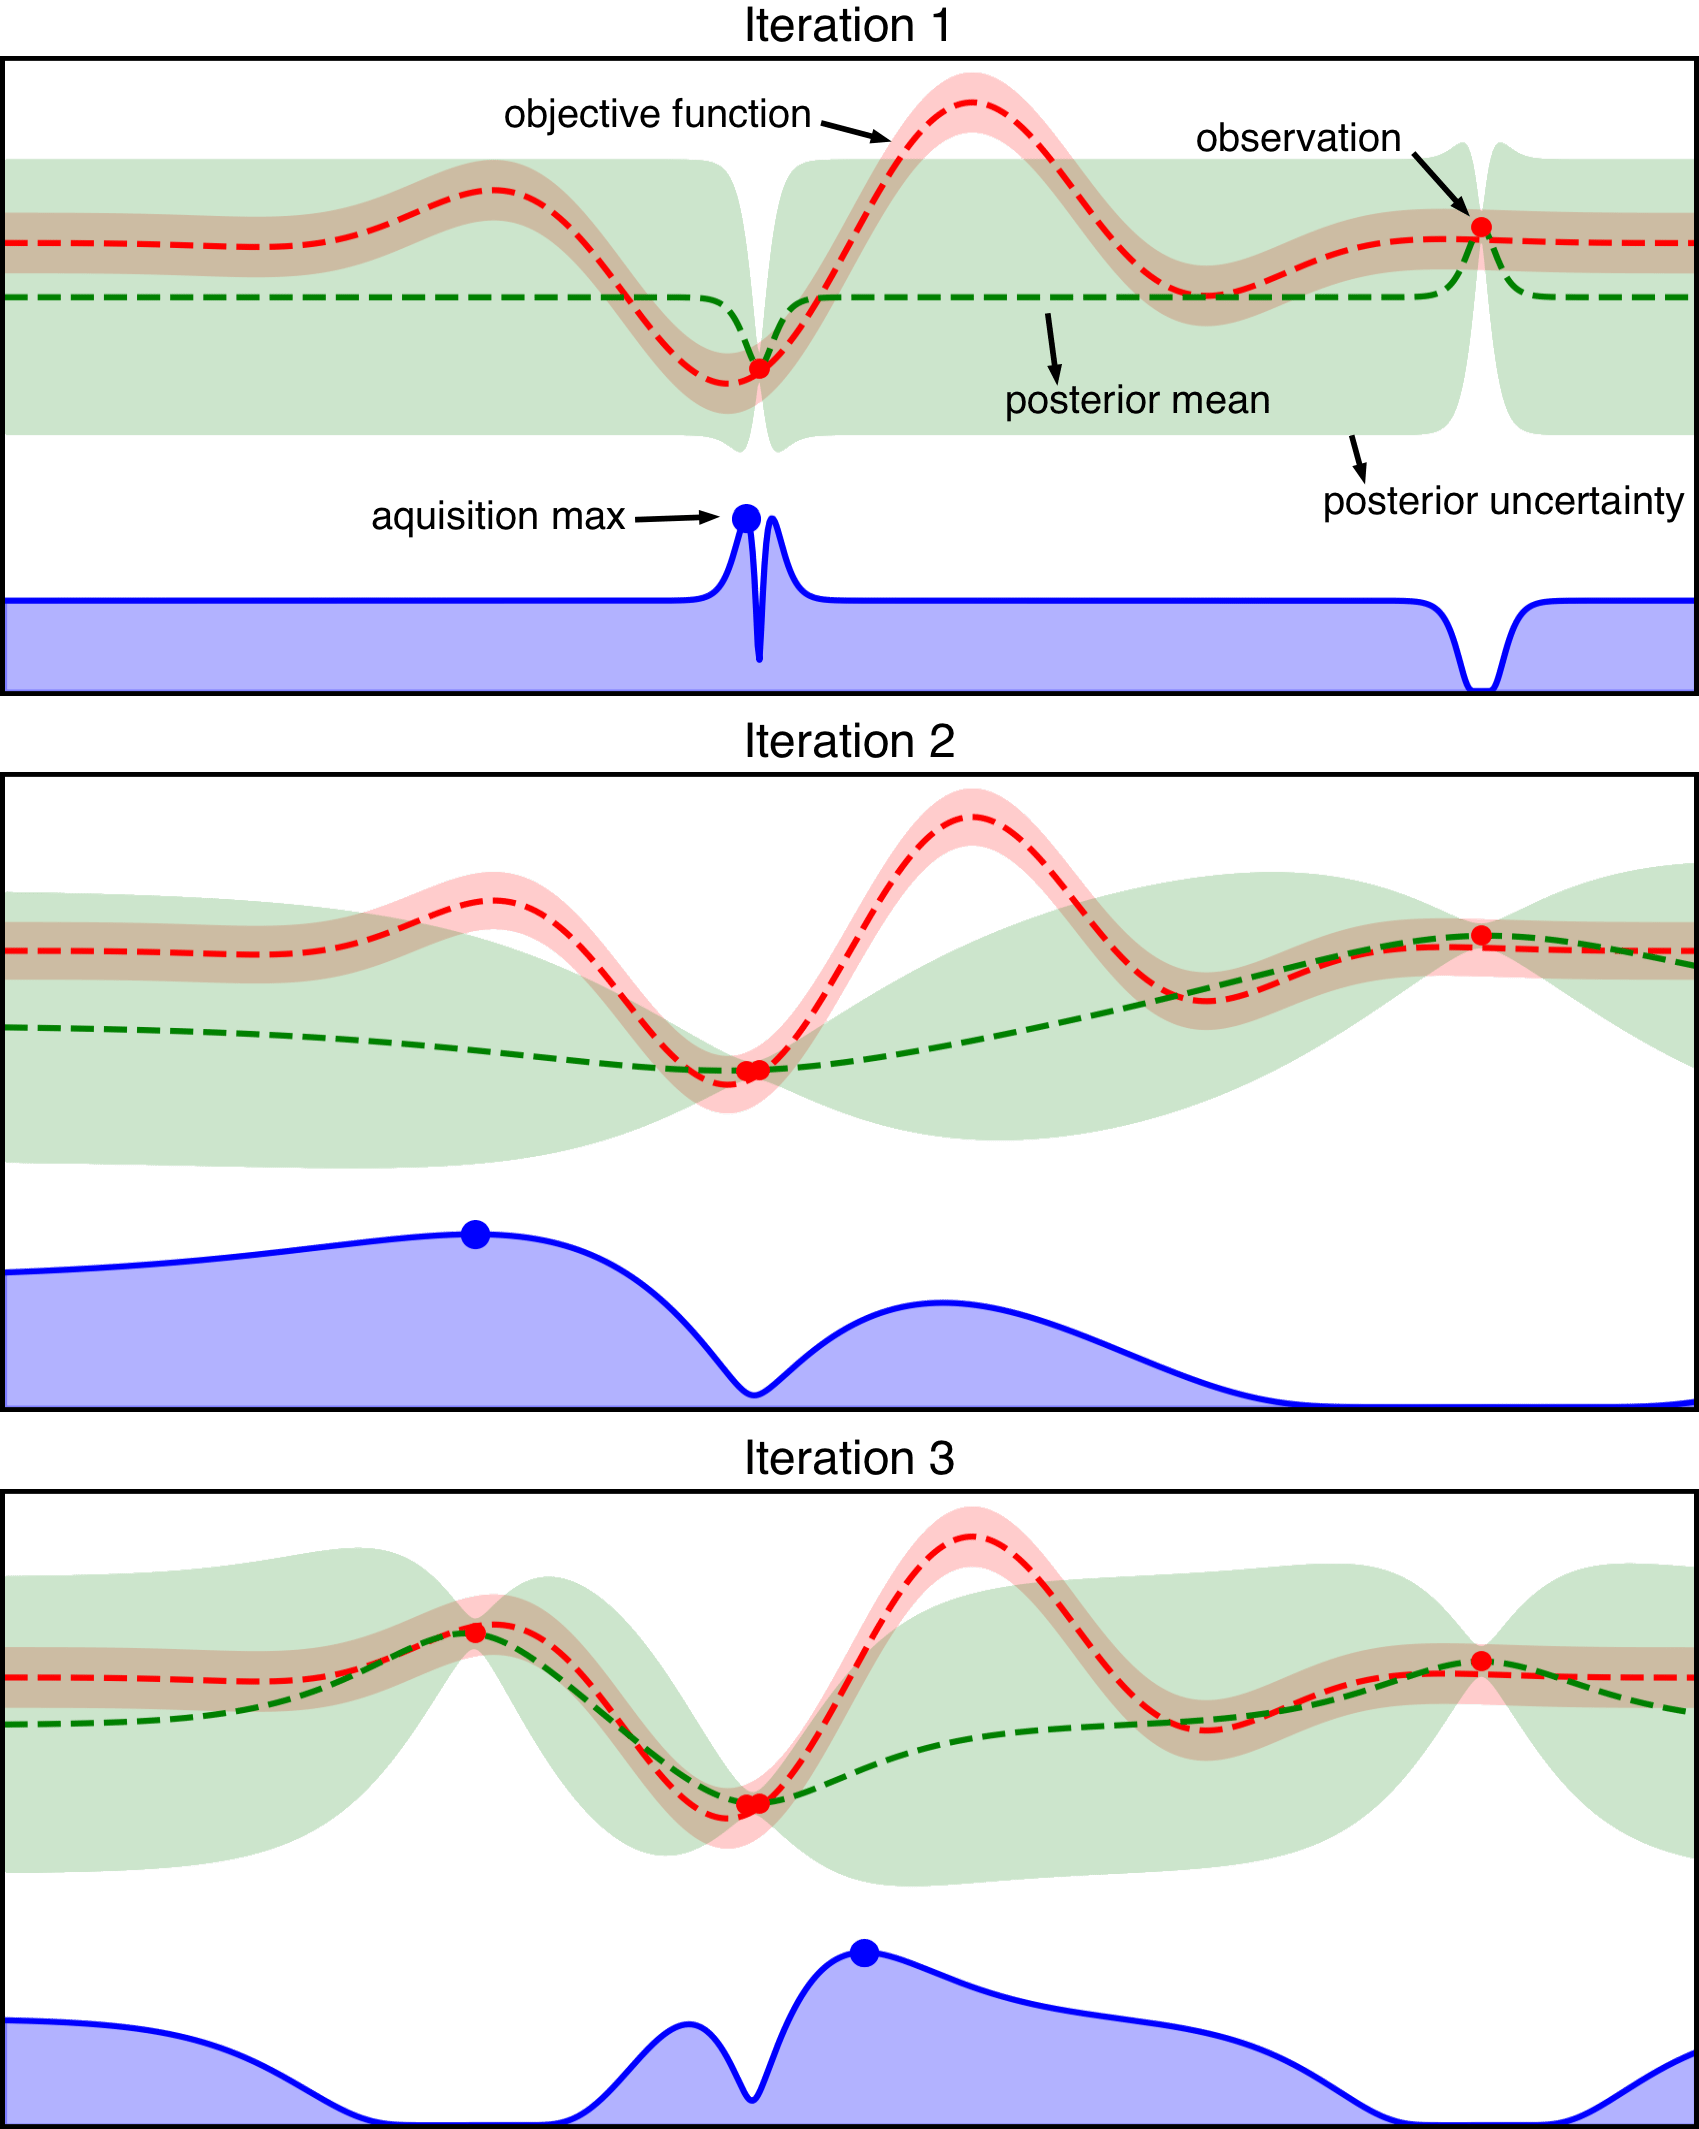
\includegraphics[width=0.7\textwidth]{bo-sample.png}
	\caption[An example of \gls{bo} using a \gls{gp} surrogate]{An example of \gls{bo} using a \gls{gp} surrogate (mean prediction as green dotted line, uncertainty as green tube) and an acquisition function (lower blue curve) on a noisy 1D toy function (red dotted line with red tube as noise).
		The figure shows three different iterations of the \gls{bo} process using two initial samples: The top shows the first iteration with only the samples to build the surrogate on and low acquisition values around these points. The middle shows the following iteration, including the newly sampled point, while reducing the uncertainty. The bottom shows that only after three iterations, almost half of the acquisition space has lost its value, and the surrogate model gains more accuracy around the samples.}
	\label{fig:bo-sample}
\end{figure}

Various combinations of surrogate model and acquisition function are possible in realizing a \gls{bo} algorithm. The relatively fast convergence to near-global optima makes this versatile algorithm a viable choice for \gls{hpo}, greatly improving on model-free methods. However, the sequential dependence on previously sampled data makes parallelization difficult \cite{yang2020hyperparameter}.
The following subsections briefly describe some popular acquisition functions and then discuss three surrogate models in more detail. These models were chosen based on their variance with respect to the \gls{bo} process. A more detailed justification is given in \cref{chap:opt-choice}.

\subsubsection{Acquisition Functions}
\label{chap:bo-acq}

As mentioned before, an acquisition function guides the sampling process, balancing exploration and exploitation. Given the distribution of the surrogate model, including its predictive mean $\mu(\mathbf{\lambda})$, its variance function $\sigma(\mathbf{\lambda})$, and the previously sampled data $\mathcal{D}$, where $f_{min} = \operatorname*{argmin}_{\mathbf{\lambda}\in \mathcal{D}} f(\mathbf{\lambda})$ is the best observed value so far, the acquisition function is defined as $u: \mathbf{\Lambda} \to \mathbb{R}^+$ \cite{snoek2012practical}. Two common choices for this function are the \gls{pi} and the \gls{ei}.

\paragraph{Probability of Improvement}
\gls{pi} as proposed by \citet{kushner1964new} attempts to maximize the probability of improving over the current best value $f_{min}$, with little regard for the comparative amount of improvement in less certain but more promising environments. With a trade-off parameter $\xi \geq 0$ to control this shortcoming, and $\Phi(\cdot)$ denoting the  \gls{cdf} of the standard normal, the resulting acquisition function is:
\begin{equation}
	\text{PI}(\mathbf{\lambda}) = P(f(\mathbf{\lambda}) < f_{min} + \xi)  
	= \Phi \left(  \frac{f_\text{min} - \mu(\mathbf{\lambda}) - \xi}{\sigma(\mathbf{\lambda})} \right) 
\end{equation}
This process is greedy by nature, but offers a guaranteed improvement of at least $\xi$ \cite{brochu2010tutorial}.

\paragraph{Expected Improvement}
As proposed by \citet{jones1998efficient}, \gls{ei} improves on \gls{pi} by also considering the magnitude of potential improvement a sample may yield. The goal is to calculate the expected deviation from a potential sample $f(\mathbf{\lambda})$ and the current minimum $f_\text{min}$, so
\begin{equation}
	\text{EI}(\mathbf{\lambda}) = \mathbb{E}[\max(f_\text{min}-f(\mathbf{\lambda}),0)].
\end{equation}
This allows the sample to be chosen to give a maximum improvement over the previous best observation.
\gls{ei} can also be expressed in a closed form with an additional trade-off parameter $\xi \geq 0$ to balance exploration and exploitation. Using the standard normal \gls{cdf} $\Phi(\cdot)$ and standard normal \gls{pdf} $\phi(\cdot)$, the equation is defined as follows:
\begin{equation}
	\label{eq:ei}
	\text{EI}(\mathbf{\lambda}) = (f_\text{min} - \mu(\mathbf{\lambda}) - \xi) \cdot \Phi(Z)+\sigma(\mathbf{\lambda})\cdot \phi(Z) 
\end{equation} 
$$
Z =  \frac{f_\text{min} - \mu(\mathbf{\lambda}) - \xi}{\sigma(\mathbf{\lambda})} 
$$
The first addend of \cref{eq:ei} realizes the exploitation of the function, favoring high means, while the second addend handles the exploration, selecting points with large surrogate variances \cite{brochu2010tutorial}.


\subsubsection{Surrogate Model: Gaussian Process}
A standard choice for a surrogate model is the \gls{gp}. As an extension of the multivariate Gaussian distribution, a \gls{gp} is defined by any finite number $N$ of variables (parameters) $\mathbf{\lambda}$, or in this case by their mean $m(\mathbf{\lambda})$, and a covariance function $k(\mathbf{\lambda},\mathbf{\lambda}^{\prime})$:
\begin{equation}
	f(\mathbf{\lambda}) \sim \mathcal{GP}(m(\mathbf{\lambda}), k(\mathbf{\lambda},\mathbf{\lambda}^{\prime}))
\end{equation}
where the mean function is most often taken to be zero, so that the process relies solely on the covariance function, whose specification assumes a distribution over the objective function \cite{williams2006gaussian}. The default choice for this so-called \textit{kernel} (implying the use of the \textit{kernel trick}) in the original proposal is a squared exponential function, which specifies the covariance between pairs of random variables $\mathbf{\lambda_i},\mathbf{\lambda_j}$ as:
\begin{equation}
	k(\mathbf{\lambda_i},\mathbf{\lambda_j}) = \exp \left(  -\frac{1}{2} \lVert \mathbf{\lambda_i} - \mathbf{\lambda_j} \rVert^2 \right) 
\end{equation}

Then, using the Sherman-Morrison-Woodbury formula, a predictive distribution for the function value at the next iteration $t+1$ can be expressed by:
\begin{equation}
	P(f_{t+1} | \mathcal{D}_t, \mathbf{\lambda_{t+1}} ) = \mathcal{N}(\mu_t(\mathbf{\lambda_t+1}), \sigma^2_t(\mathbf{\lambda_t+1}))
\end{equation}
where $\mu$ and $\sigma^2$ denote the mean and variance of the model, and can be calculated using the kernel matrix over the covariance function (see \cite[p.8]{brochu2010tutorial}).
A disadvantage of the squared exponential kernel is that it assumes a very smooth objective function, which is unrealistic for real physical processes \cite{stein1999interpolation}.  
Instead, a Matérn kernel is often suggested as a replacement. It uses a parameter $\upsilon$ to control  smoothness, and common settings for \gls{ml} applications are $\upsilon = 3/2$ and $\upsilon=5/2$ \cite{williams2006gaussian}.

The default \gls{gp} scales cubically with the number of data points, which limits the number of function evaluations. Another issue is poor scalability to higher dimensions, which is attempted to be overcome by using other kernels \cite{feurer2019hyperparameter}.


\subsubsection{Surrogate Model: Random Forest}
\label{chap:rf}
Very different from \gls{gp} are the next two approaches, which come from the field of ensemble methods often used in \gls{ml}. The basic idea of these methods is to train several so-called \enquote{base learners} $h_1(\mathbf{\lambda}), ...,h_J(\mathbf{\lambda})$ (sometimes also referred to as \enquote{weak learners}), which are easy to fit and infer on, but have poor individual generalization performance due to very high variance. The base learners are then combined to produce a final predictor of the objective function $\hat{f}(\mathbf{\lambda}) (\approx f(\mathbf{\lambda}))$. In the case of regression, which applies to \gls{hpo}, this means a simple average of all base learners \cite{cutler2012random}:
\begin{equation}
	\label{eq:avg-est}
	\hat{f}(\mathbf{\lambda}) = \frac{1}{J} \sum_{j=1}^{J} h_j(\mathbf{\lambda})
\end{equation}

\gls{rf} is one of these methods, and was first introduced under this name by \citet{breiman2001random} as an improvement on his bagging algorithm for decision trees.
Each base learner, as described above, is a binary partitioned regression tree, where each partition or \enquote{split} is based on a predictor variable $\lambda_i \in \mathbf{\lambda}$ (i.e., the hyperparameters). A split may be done by value range for a continuous variable, or by choosing a subset $S$ from the set of all categories $S_i$ for categorical variables (see \Cref{fig:decision-tree}). A splitting criterion is used to evaluate all possible splits among all variables, and then the most descriptive split is chosen. For regression, the mean squared error is often used for this task, while classification typically uses the Gini index to calculate the \enquote{purity} of each potential class \cite{cutler2012random}. 

\begin{figure}
	\centering
	\resizebox{0.9\textwidth}{!}{
		\begin{forest} decision tree
			[$\lambda_i < a$,plain content
			[left descendant;{yes},plain content,elo={yshift=2pt}]
			[right descendant;{no},plain content,elo={yshift=2pt}]
			]
		\end{forest}
		\quad
		\begin{forest} decision tree
			[$\lambda_i \in S \subset S_i$,plain content
			[left descendant;{yes},plain content,elo={yshift=2pt}]
			[right descendant;{no},plain content,elo={yshift=2pt}]
			]
	\end{forest}}
	\caption[Example of decision trees]{Example of two decision trees. (Left) Splitting a continuous variable $\lambda_i$ at point $a$. (Right) Splitting a categorical variable $\lambda_i$ via subset $S$.}
	\label{fig:decision-tree}
\end{figure}

The bagging algorithm now improves on the foundation of decision trees \cite{breiman1996bagging}. Given a data set $\mathcal{D}$ of size $n$, consisting of pairs of $N$ parameters $\mathbf{\lambda} = \left\lbrace \lambda_1,...,\lambda_N\right\rbrace $ and their corresponding function value $y = f(\mathbf{\lambda})$, bagging repeatedly selects a random subset of the same size $n$ as the original data set, but with replacement, thus allowing for duplicates and possible unused values or \enquote{out-of-bag} data. This process is called \enquote{bootstrap sampling} and reduces overfitting, while also allowing the out-of-bag data to be used to validate the estimator. The tree is then fitted using this sample as described above.

\gls{rf} introduces more randomization into the decision tree building process by taking not only a subset of the available data for each base learner, but also taking a random sample (with replacement) of size $m$, where $m < N$ of the predictor values for each split. As a result, the base learners do not overfit to presumably highly predictive variables, which reduces the correlation among the sub-sampled data sets and increases the accuracy of the ensemble prediction \cite{ho2002data}. The resulting implementation template is described in \cref{alg:random-forest}. The process can also be easily parallelized since each base learner is constructed individually \cite{cutler2012random}.

\begin{algorithm}
	\caption{Random Forests}
	\label{alg:random-forest}
	\begin{algorithmic}
		\For{$j=1$ to $J$}
			\State $\mathcal{D}_j \subseteq \mathcal{D}$ \Comment{sample with replacement, $|\mathcal{D}_j| = |\mathcal{D}|$}
			\Procedure{CreateTree}{$\mathcal{D}_j, m$} $ \to h_j(\mathbf{\lambda})$
				\State Start with all observations in root node
				\ForAll{unsplit nodes, recursivley}
					\State Randomly select $m$ predictor variables
					\State Split the node according to the best binary split among these $m$ variables
				\EndFor
			\EndProcedure
		\EndFor
		\Return $\hat{f}(\mathbf{\lambda})$ \Comment{using \cref{eq:avg-est}}
	\end{algorithmic}
\end{algorithm}

\paragraph{Extremely Randomized Trees}
As the name suggests, the extremely randomized trees approach proposed by \citet{geurts2006extremely} introduces another step of randomization into the process. While the main part of this algorithm, often called \gls{et}, is based on random forests, the split points for each node of the decision tree are now chosen completely randomly, as opposed to being based on the best split among all available predictor variables. To explain further, the sampled $m$ predictor variables are each randomly split once, evaluated (e.g., using the mean squared error), and then the best performing split is chosen for the current node. In addition, each base learner is now built using the entire data set, rather than just a bootstrap sample. The motivation behind \gls{et} is to reduce variance through random splits and minimize bias by using the full data set, while also having the potential to improve the computational time needed to build the estimator.

\subsubsection{Surrogate Model: Gradient Boosted Trees}

\gls{gbrt} is also an ensemble method that uses decision trees as base learners to produce an ensemble prediction, and was originally proposed by \citet{friedman2001greedy}. However, unlike \gls{rf}, which averages many full-depth decision trees, \gls{gbrt} sequentially builds many small, high-bias decision trees (depth $d \approx 4$), improving on each other using the residuals from the last iteration. The schematic architecture of this approach is outlined in \cref{fig:gbrt}.
\begin{figure}
	\centering
	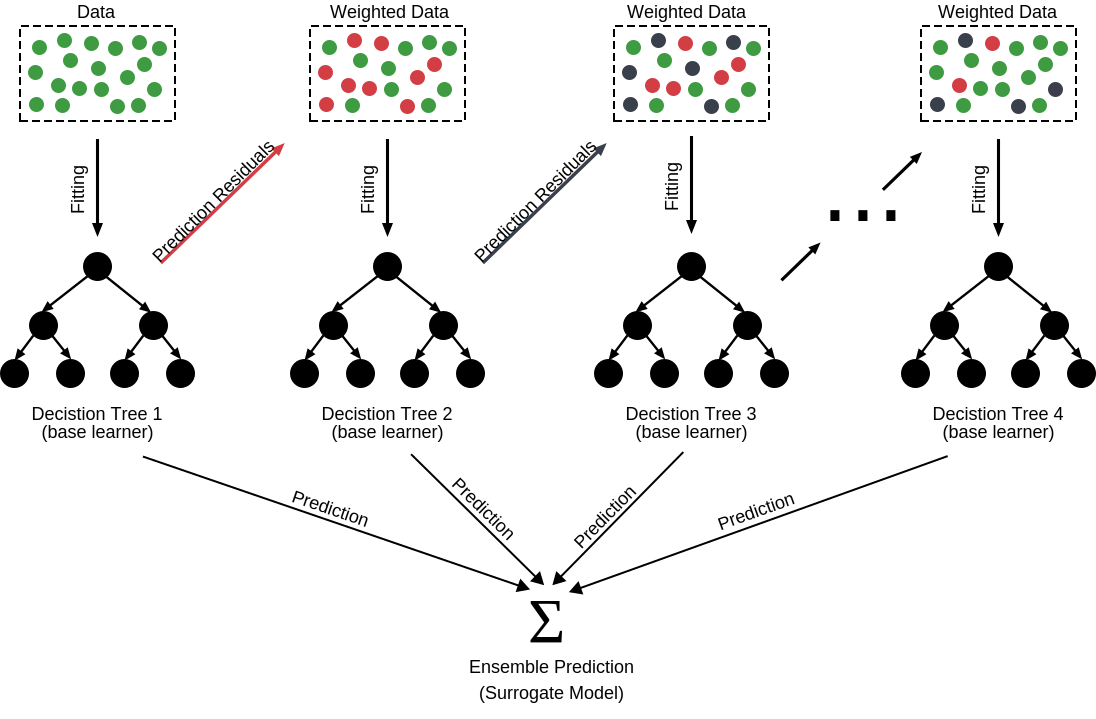
\includegraphics[width=\textwidth]{gbrt.svg}
	\caption[Schematic view of \gls{gbrt}]{Schematic view of \gls{gbrt}. Modified from \citet{deng2021ensemble}.}
	\label{fig:gbrt}
\end{figure}
For simplicity, let $f_j = f_j(\mathbf{\lambda})$. The ensemble regressor $\hat{f}_j$ is the $j$-th of all $J$ estimators in an additive sequence 
\begin{equation}
	\label{eq:add-gbrt}
	\hat{f}_j = \hat{f}_{j-1} + \upsilon \cdot h_j
\end{equation}
where $\upsilon \in (0,1]$ is a \enquote{shrinkage} parameter that controls the learning rate, leading to better generalization \cite{friedman2002stochastic}.
Let $\mathcal{L}(f,\hat{f})$ be the loss function for the estimator. Now, at each iteration $j$, a new base learner $h_j$ is added to the ensemble by minimizing over its sum of losses for the entire data set $\mathcal{D}$ ($|\mathcal{D}| = n$), with $(\mathbf{\lambda}_i, y_i)$ being the $i$-th element of $\mathcal{D}$\footnote{Note that this is an exception to the previously established notation that $\mathbf{\lambda}_i$ is the $i$-th parameter in the configuration.} and $y_i = f(\mathbf{\lambda}_i)$ \cite{friedman2001greedy}:
\begin{equation}
	\label{eq:gbrt-tree}
	h_j = \operatorname*{argmin}_{h} \sum_{i=1}^{n} \mathcal{L}(y_i, \hat{f}_{j-1}(\mathbf{\lambda}_i) + h(\mathbf{\lambda}_i))
\end{equation}
To make this a computationally closed-form, a first-order Taylor approximation to the loss-function is used to obtain the following term:
\begin{equation}
	\mathcal{L}(y_i, \hat{f}_{j-1}(\mathbf{\lambda}_i) + h(\mathbf{\lambda}_i)) \approx \mathcal{L}(y_i, \hat{f}_{j-1}(\mathbf{\lambda}_i)) + h_j(\mathbf{\lambda}_i) \left[ \frac{\partial\mathcal{L}(y_i, \hat{f}(\mathbf{\lambda}_i))}{\partial \hat{f}(\mathbf{\lambda}_i)} \right]_{\hat{f}=\hat{f}_{j-1}}
\end{equation}
The derivative of this equation can be understood as the gradient $g_{ij}$ of the loss function, where a steepest descent following $-g_{ij}$ is desired. To summarize, in each of the $J$ iterations, a decision tree of fixed depth $d$ is fitted using all predictor variables to minimize the negative gradient of the all $n$ data points:
\begin{equation}
	h_j \approx -\operatorname*{argmin}_{h} \sum_{i=1}^{n} (h(\mathbf{\lambda}_i) - g_{ij})^2
\end{equation}
Given a typical squared error loss function $\mathcal{L}(f, \hat{f}) = \frac{1}{2}(f - \hat{f})^2$, the negative gradient can be simplified to an ordinary residual $r_{ij} = -g_{ij} = y_i - \hat{f}_{j-1}(\mathbf{\lambda}_i)$ \cite[Chapter~10]{hastie2009elements}.

Lastly, \cref{alg:gbrt} describes the high-level implementation of \gls{gbrt} using a squared loss function and a decision tree building process, as described with \gls{rf} in \cref{chap:rf}, using a continuous update for the residuals ($r_{i} \gets r_{ij}$, for current iteration $j$) \cite{mohan2011web}.
Although this algorithm uses a constant initialization for the residuals, other methods could be used as well.

\begin{algorithm}
	\caption{Gradient Boosted Regression Trees (Squared Loss)}
	\label{alg:gbrt}
	\begin{algorithmic}
		\State Initialization: $\forall i \in [1,n]: r_i = y_i$
		\For{$j=1$ to $J$}
			\State$h_j \gets$ \Call{CreateTree}{$\left\lbrace (\mathbf{\lambda_1}, r_1), ..., (\mathbf{\lambda_n}, r_n)\right\rbrace$, $d$}
			\For{$i=1$ to $n$}
				\State $r_i \gets r_i - \upsilon \cdot h_j(\mathbf{\lambda_i})$
			\EndFor
		\EndFor
		\State $\hat{f} = \upsilon \cdot \sum_{j=1}^{J} h_j$
		\State \Return $\hat{f}$
	\end{algorithmic}
\end{algorithm}


\subsection{Example: Bayesian Optimization for the H-SPPBO}
To better understand how the \glsdesc{hpo} process works with a metaheuristic such as the \gls{hsppbo}, the following is a theoretical example using the mathematical symbols and formula from above. This example focuses on \gls{bo} using a \gls{rf} surrogate model, and the underlying problem to be solved is the \gls{tsp}.

Let the \gls{hsppbo} algorithm, as explained in \cref{chap:hsppbo}, be denoted by $\mathcal{A}_\mathbf{\lambda}$ with its parameters initialized by the parameter vector $\mathbf{\lambda}$. This parameter vector is an element of the parameter configuration space $\mathbf{\Lambda} = \Lambda_1 \times \Lambda_2 \times ... \times \Lambda_N = w_{\text{persprev}} \times w_{\text{persbest}} \times w_{\text{parentbest}} \times \alpha \times \beta \times \theta \times H \times L$. Furthermore, let each solution constructed by $\mathcal{A}_\mathbf{\lambda}$ be defined as a vector $\mathbf{s} = (s_1,...,s_n) \in V^n$, where $V$ is the set containing all possible city nodes of the \gls{tsp} problem description. Assuming, that random influences can be ignored, the function describing this solution construction depends only on the parameters and is denoted as $g(\mathbf{\lambda}) = \mathbf{s}$. The quality of each solution $f : V^n \rightarrow \mathbb{R}_{0}^{+}$ is then defined as the tour length $L$ given by the weights/distances between each of the nodes, described by \cref{eq:solution_quality}, so $f(\mathbf{s}) = L$. Since these solutions are depend only on the parameters $\mathbf{\lambda}$ with which the \gls{hsppbo} algorithm $\mathcal{A}_\mathbf{\lambda}$ was initialized, again assuming no random influences, the function definition  $\mathbf{\lambda} \to_{g} V^n \to_{f} \mathbb{R}_{0}^{+}$ can be simplified to directly output the length $L$ for any given parameter vector $\mathbf{\lambda}$. Thus, the only function necessary for the metaheuristic is now defined as $f(\mathbf{\lambda}) = L = y$, where $y$ is used to conform to the previous notation for \gls{hpo}.

Now, given the \glsdesc{hpo} goal from \cref{eq:hpo-meta}, we have defined the solution quality function $f$ and the algorithm $\mathcal{A}_\mathbf{\lambda}$, as well as a configuration space $\mathbf{\Lambda} $. In addition, let $F(\mathbf{\Lambda})$ denote a sampling function that chooses a parameter set $\mathbf{\lambda}$ under a uniform distribution, let $u: \mathbf{\Lambda} \to \mathbb{R}^+$ be an arbitrary acquisition function, and let $\mathcal{D}_t = \left\lbrace (\mathbf{\lambda_i}, y_i) |  i\in [1,t] \right\rbrace $ be the data set consisting of the parameter pairs and their corresponding solution qualities, sampled so far during the \gls{hpo} process.

Starting with the \gls{bo} process, we first obtain an initial data set $\mathcal{D}_\text{init}$ using our sampling function $F(\mathbf{\Lambda})$. For example, the first entry of this set might contain, among the other parameters, the two values $\alpha = 8, \beta = 2$, resulting in a solution quality (tour length) of $y = 100$, and a second entry might contain the values $\alpha = 7, \beta = 3$, resulting in a solution quality of $y=90$, so $\left\lbrace ((...,8,2,...), 100), ((...,7,3,...), 90) \right\rbrace \subset \mathcal{D}_\text{init}$. Based on this data, the first \gls{rf} model is built as explained in \cref{chap:rf}. For example, the first base learner $h_j(\mathbf{\lambda})$ built in the ensemble of all $J$ learners could select $\alpha < 7.5$ as a split node for the decision tree with a predicted solution quality of $y=100$ for the side where the condition is true, and $y=90$ otherwise. This split was chosen because following the prediction of this decision tree using the parameters from the data set $\mathcal{D}_\text{init}$ resulted in the lowest mean squared error of all possible splits. Note, that this explanation is an oversimplification of the actual process. 

From this split, all further child nodes are also split until some termination criterion is met, e.g. the mean squared error is below a certain threshold. Now that we have trained our base learners, we average over their predictions, resulting in our predictor $\hat{f}(\mathbf{\lambda}) = \hat{y}$. This predictor, or surrogate model in terms of the \gls{bo}, is ideally as close as possible to the actual objective function $f(\mathbf{\lambda}) = y$ that we defined earlier. However, the predictor only learns a relationship between an input parameter set and the resulting solution quality (tour length $L$), not the actual solution path $\mathbf{s}$. Ignoring possible \gls{ml}-related effects such as overfitting, the more parameter pairs and corresponding solution qualities we have, the more accurate our predictor will be. Nevertheless, since we do not want to run hundreds or thousands of expensive real objective function calls, we use the \gls{bo} process, to acquire only new data points that maximize our benefit for training this predictor - quality over quantity of data.

As we progress in the \gls{bo} process, we can use our trained surrogate model for the acquisition function $u(\cdot)$ to determine the most beneficial new point in the parameter configuration space $\mathbf{\Lambda}$. To do this, we need to compute the mean and variance over our surrogate model and its parameter inputs (see \cref{chap:bo-acq}). The resulting new point from $u$, which is a parameter set $\mathbf{\lambda}$, is evaluated by the real objective function, the \gls{hsppbo}, and this new data point $(\mathbf{\lambda}, y)$ is added to $\mathcal{D}_t$ in the $t$-th iteration of the \gls{bo} algorithm (see \cref{alg:bo}). The \gls{rf} surrogate model is then trained again, but now with this new data point, which should increase its accuracy. This process is repeated until a certain number of predetermined objective calls (\texttt{n\_calls}) have been evaluated. Finally, the \gls{bo} algorithm returns the parameter set $\mathbf{\lambda}^*$ from the iteration that produced the best solution quality $y$. We also get the final trained surrogate model $\hat{f}(\mathbf{\lambda})$.

% !TeX root = main.tex
% !TeX spellcheck = en-US
% !TeX encoding = utf8


\chapter{Implementation}
\label{chap:implementation}
\glsreset{hsppbo}
\glsreset{hpo}
\glsreset{bo}

\epigraph{A tool that does everything is optimized for nothing.}

\section{Modules}
\label{chap:modules}

The implementation used for all the experiments in this thesis combines several theoretical aspects of \cref{chap:background}. The foundation, of course, is the \gls{hsppbo} algorithm implemented as explained in \cref{chap:hsppbo}. Then a \gls{hpo} framework using \gls{bo} was built around this algorithm, along with several other modes of operation that make use of the metaheuristic algorithm. Although, the package is mostly adaptable to other combinatorial problem types, it has some aspects to it that were designed with the \gls{dtsp} in mind. These are highlighted as such.

\begin{figure}[h]
	\centering
	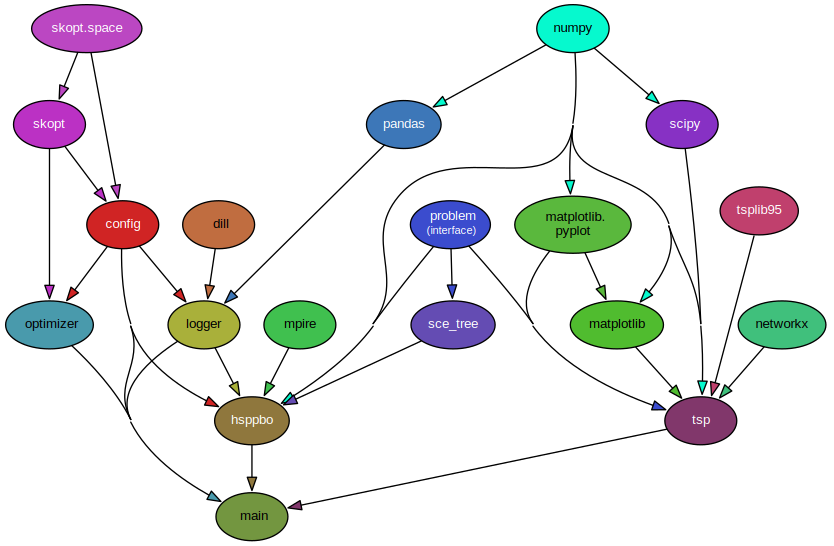
\includegraphics[width=0.95\textwidth]{code-dependency.svg}
	\caption{Dependency graph of the \textit{XF-OPT/META} python software package}
	\label{fig:dependency}
\end{figure}

The entire program package was written in \textit{Python}, with some modules completely imported from established libraries (especially for \gls{ml} and statistical functionality), some modules consisting of modified libraries that did not quite meet the requirements, and some completely new modules. \Cref{fig:dependency} shows the dependency graph starting from the \texttt{main} function, with a maximum depth of three references. 
These modules, their dependencies, and their general functionality are individually explained in the following subsections to provide a better understanding of the experiments and the research process.

\subsection{H-SPPBO Module}
\label{chap:hsppbo-module}
The \texttt{hsppbo} module implements a multiprocessing version of the \gls{hsppbo} algorithm (see \ref{alg:hsppbo}). It is initialized using all the parameters discussed in \cref{chap:hsppbo}:
\begin{itemize}
	\item The three weights $w_{\text{persprev}}, w_{\text{persbest}}, w_{\text{parentbest}} \geq 0$ controlling the influence of their respective populations
	\item $\alpha, \beta \geq 0$ limiting the influence of the stochastic and the heuristic importance
	\item A detection threshold $\theta \in [0,1]$
	\item A categorical dynamic reaction type $H = \left\lbrace H_{\text{full}}, H_{\text{partial}}, \emptyset \right\rbrace$
	\item A number of iterations to pause detections for $L_\text{pause} > 0$
	\item A maximum number of iterations $i_{\text{max}}$ (used as a termination criterion).
\end{itemize}

In addition, some parameters have been fixed in the code using the suggestions from the original paper \cite{kupfer2021hierarchical}. The number of \glspl{sce} is set to $|\mathcal{A}| = 13$ with three children per \gls{sce}. The weight for the random influence $w_\text{rand}$ is set to $\frac{1}{n-1}$ where $n$ is the dimension of the \gls{tsp} instance\footnote{This value may not be ideal for other problem types.}.

Since the algorithm is influenced by many random processes, it explicitly provides a function to manually set a random seed, i.e. every time a random number is drawn or something is chosen from a probability distribution, we can expect the same outcome. This not only makes personal benchmarking more comparable, but also allows reproducible solutions, which is a very important aspect in \gls{ml} research. The use of this feature for the experiments is discussed further in \cref{chap:testing}.

The solution construction process is implemented in a sequential, iterative manner, similar to the description around \cref{eq:hsppbo_prob}. An attempt to convert this task into a matrix computation problem, using the capabilities of the popular \textit{NumPy} \cite{harris2020array} library, resulted in worse or similar performance at best. Hence, this approach was not followed in order to reduce complexity.
As a result, the computational performance of the solution construction process relies heavily on the calculations of $s_{ik}(P)$, which is basically a lookup of a subset in an ordered set (see \cref{ex:subset}).
For this reason, a key-value hash-map (called \texttt{dictionary} in \textit{Python}) was used as the solution population $P$ and a write-once, read-many tuple was used for the potential subset. The crucial function is the following:
\begin{Listing}[h]
	\begin{minted}{python}
		
def is_solution_subset(subset: tuple, solution: dict) -> bool:
  try:
    return solution.get(subset[0]) + 1 == solution.get(subset[1])
  except:
    return False
	\end{minted}
	\caption{The \textit{Python} code for the check, if a set is a subset of an ordered subset.}
	\label{lst:subset}
\end{Listing}

This code works well for two important reasons.
First, in the case of the \gls{tsp}, the solution is essentially just a list of node identifiers of size $n$. Since these are the keys, the values are just their indices in this list.
Second, \texttt{dictionaries} have a great key lookup performance. The \texttt{get}-method returns the value of the given key.
Thus, using the first node of the subset as the dictionary key returns its index in the solution sequence. Therefore, adding one to this index and checking again for the index of the second node in the subset should result in equality, if the subset exists. 
Many other solutions have been tried, some not specific enough for this use case, others not focused on performance. This small function was the result of many optimization efforts and the complete creation process scales linearly with $n$. Every iteration, a total number of $|\mathcal{A}| = m$ solutions are created, which gives a worst case time complexity of $\mathcal{O}(n^m)$.

Other performance improvements are achieved through parallelization. During the solution creation and population update procedure, each \gls{sce} operates individually, with only the parent best solution as a reference. Therefore, this process is parallelized using the \texttt{mpire} library \cite{mpire2023} for problem dimensions $n > 100$. Smaller instances of the \gls{tsp} were sequentially fast enough to outperform their parallelized counterparts because the overhead to do so was greater than the gain in performance.

\subsubsection{SCE Tree Module}

The \glspl{sce}, their populations $P^A_{\text{persprev}}$,$P^A_{\text{persbest}}$ and the tree structure are encapsulated in their own module \texttt{sce\_tree}, which is an extensions of the $k$-ary tree package \texttt{treelib} \cite{chen2018treelib}.
We have separate classes for the tree (\texttt{SCETree}) and its nodes (\texttt{SCENode}). Each node is essentially an \gls{sce} $A \in \mathcal{A}$ and holds four variables:
\begin{itemize}
	\item $P^A_{\text{persprev}}$ (tuple): Previous solution of the SCE node
	\item $f(\mathbf{s}^A_{\text{persprev}})$ (float): Quality of the personal pervious solution
	\item $P^A_{\text{persbest}}$ (tuple): Personal best solution of the SCE node
	\item $f(\mathbf{s}^A_{\text{persbest}})$ (float): Quality of the personal best solution
\end{itemize}

The output of the solution quality function $f(\cdot)$ depends on the provided problem type and module, as well as the initialization of the solutions for the populations. This module and the specific case of the \gls{tsp} is explained in \cref{chap:impl-problem}.
After each \gls{sce} node is initialized, they are ordered into an $k$-ary tree, where $k = 3$ is the number of children each parent has. The structure is similar to \cref{fig:ternary-tree}.
The \texttt{treelib} base package already provides much of this functionality, but the swapping of the \glspl{sce} had to be implemented separately.
In addition, the algorithm-specific change handling procedures are also present in this module, either resetting the personal best solution of the whole tree ($H_{\text{full}}$) or only from the third level down ($H_{\text{partial}}$).

\subsection{Problem Interface}
\label{chap:impl-problem}

The \texttt{problem} module is implemented as an interface for all kinds of problem realizations. It uses \textit{Python}'s abstract methods to facilitate future development of other (dynamic) problem types, and provides guidance on all important methods, their parameters and return values. All other modules only use their problem instance through this interface, which further simplifies development.
Although the problem module should also contain the functions to validate, randomly generate, and evaluate its corresponding solutions, it does not store these solutions.

One of these problem types using the interface is the \texttt{tsp} module, which implements the symmetrical \gls{tsp} with optional dynamic capabilities to turn every instance into a \gls{dtsp} problem.

\subsubsection{TSP Module}
\label{chap:tsp-module}

The \texttt{tsp} module is a realization of the problem described in \cref{chap:tsp-theory}. Programmatically, it is based on the \texttt{tsplib95} library, which provides read, write, and transform functions for files in the \texttt{.tsp} file format proposed by \citet{reinelt1991tsplib}. It works very well with \gls{tsp} instances of the types \textit{EUC\_2D} (cities in a two-dimensional Euclidean space), \textit{GEO} (cities as geographic coordinates), and \textit{ATT} (special pseudo-Euclidean distance function), thus limiting the capabilities to these types.

The specific \gls{tsp} instance is initialized by its name (e.g., \texttt{rat195}) and then loaded by \texttt{tsplib95}. From this instance, the dimension $n$ is stored and the distance matrix $D$ is calculated using the package's Euclidean distance method and \texttt{numpy} \cite{harris2020array}.
Since all solutions generated by the \texttt{tsp} module are of the same type, they share a solution quality function $f : V^n \rightarrow \mathbb{R}_{0}^{+}$. It works as described in \cref{chap:hsppbo}, where each solution vector $\mathbf{s}$ is given as a $n$-dimensional combination of the solution space $V$, where the positive real value is the length of the traveled tour $L$.

The \gls{dtsp} is implemented by enabling the positional swap of two randomly selected city nodes.
This dynamic part of the problem is optional and can be initialized separately. The settings correspond to those of \citet{kupfer2021hierarchical} and are as follows:
\begin{itemize}
	\item A percentage $C \in [0,1]$ of how many cities $n$ are changing per dynamic turn
	\item A dynamic period $T_{d} \in \mathbb{N}$ defining how often the change is triggered
	\item A number of minimum iterations $i_{\text{min}}$ before the dynamic starts to trigger
\end{itemize}
This means that starting at iteration $i_{\text{min}}$, every $T_{d}$ iterations ($i_{\text{min}} + k \cdot T_{d} < i_{\text{max}}, k \in \mathbb{N}$) a number of $\frac{n\cdot C}{2}$ distinct pairs of cities are randomly selected and their entries in the distance matrix $D$ are swapped. After this procedure, the distance matrix is recalculated to reflect the changes.

To evaluate the problem instance itself, some statistical methods have been implemented. First, the length of the optimal solution to each symmetric \textit{TSPLIB} problem is stored in a metadata file. In addition to this information, the module can compute the mean and median distance of a problem, the standard deviation and the coefficient of variation for the distance, as well as the first eigenvalue, the \gls{cqv}, and a so-called regularity index according to \cite{clark1954distance, cricsan2021randomness, dry2012clustering}. More on the use of these values in \cref{chap:classification}.
Finally, the \gls{tsp} instances and their solutions can also be visualized using the \texttt{networkx} package \cite{hagberg2008exploring} (for an example, see \cref{fig:cluster-groups}).


\subsection{Optimizer Module}
\label{chap:optimizer}

Several options for the \gls{hpo} module were considered, but the requirements called for an adaptable library that was not too closely tied to \gls{ml} application. Self-implementation was omitted early on to reduce complexity and potential for error. The libraries compared by \citet{yang2020hyperparameter} were reviewed and checked for potential use with metaheuristics. Ultimately, the \texttt{scikit-optimize} library \cite{head2020scikit} was chosen as the most versatile and adaptable option, while still providing reasonable performance. In addition to the basic \gls{rs} method, it also gives an implementation of \glsdesc{bo} with several options for surrogate models: \gls{gp}, \gls{rf}, \gls{et}, and \gls{gbrt} (see \cref{chap:bo} for details). And since \texttt{scikit-optimize} is built on top of the popular \gls{ml} library \texttt{scikit-learn} \cite{scikit-learn2011}, it allows other  regression models from that library to be used instead. Furthermore, it also provides three popular acquisition functions - \glsfirst{pi}, \glsfirst{ei} and lower confidence bound (LCB) - of which the two explained in \cref{chap:bo-acq} were used for the experiments of this thesis.
Overall, \texttt{scikit-optimize} provides the mature interfaces and development foundation of \texttt{scikit-learn}, while also implementing a customizable \glsdesc{bo} workflow.

Because of this already good base library, the actual implementation of the \texttt{optimizer} module only contains some interfaces to streamline the interaction between the metaheuristic (in this case \gls{hsppbo}) and the \gls{hpo} process. On initialization, the optimizer class needs only three things: 
First is the optimization algorithm to use. As mentioned earlier, these are \glsdesc{rs}, \glsdesc{rf}, \glsdesc{gp}, \glsdesc{rf}, \glsdesc{et}, and \glsdesc{gbrt}. However, the choice of acquisition function and other algorithm-specific parameters have been preconfigured or left default, depending on the algorithm, which is explained in \cref{chap:opt-init}.
The second parameter for the optimizer is a reference to the execution object of the objective function $f(\mathbf{\lambda})$. \textit{Python} allows for complete methods to be used as function parameters. Therefore, the \texttt{hsppbo} module needed only a special wrapper function that accepts a variable array of parameters $\mathbf{\lambda}$, executes the algorithm with these parameters initialized for all $i_{\text{max}}$ iterations, and then returns only the quality of the best solution. Mathematically, the entire \texttt{hsppbo} module has been reduced to the function $f: \mathcal{\mathbf{\Lambda}} \to \mathbb{R}$, as explained in \cref{chap:bo}.
The third and final parameter is the configuration space $\mathcal{\mathbf{\Lambda}}$. It consists of a list of tuples, where each tuple contains the name of the parameter in the \texttt{hsppbo} module, and its domains and value ranges to be optimized.

After this initialization, the \texttt{optimizer} instance can be invoked to perform any number $r_{\text{opt}}$ of repeated optimizer runs. Each optimizer run consists of a number of calls to the objective function $f$ (denoted as \texttt{n\_calls}), where each \texttt{n\_call} uses a different parameter set bounded by the specified configuration space $\mathcal{\mathbf{\Lambda}}$ and chosen by the acquisition function $u$ (see \cref{chap:bo-acq}). The random state can also be fixed with the same reasoning as for the \texttt{hsppbo} module. After these \texttt{n\_calls} of \gls{hpo} execution, the \texttt{optimizer} module returns a result object containing, among other things, the best parameter set it obtained and the corresponding solution quality, the complete parameter history, and, if used, the trained, underlying regression model. These results, for each optimizer run $i =1,...,r_{\text{opt}}$, are collected in a set $\mathcal{C}$.


\subsection{Logger Module}

The \texttt{logger} module captures all the intermediate data and results from the \gls{hsppbo} algorithm and the \texttt{optimizer} module. It is initialized according to the operating mode (see \cref{chap:mop}) and automatically creates the necessary folder structure. Then, it outputs an info log about all the environment data concerning the \texttt{hsppbo}, \texttt{sce\_tree}, \texttt{problem}, and the \texttt{optimizer} module to precisely capture the runtime conditions of the program. In the case of an optimizer run, it also saves the complete results, including the trained regression model, in a so-called \enquote{pickle} file using the \texttt{dill} package \cite{mckerns2012building}. This package is an extension of the popular \texttt{pickle} library for serializing and deserializing \textit{Python} objects and adds support for more complex data types to be stored. This way, the various results of the \texttt{optimizer} module can be loaded and used in their entirety at any time, rather than after the run with the in-memory object still present.
This greatly improves the analysis process and allows for more complex, flexible post-processing of the data (see \cref{chap:analysis} for more details).

\section{Framework View and Workflows}
\label{chap:workflow}

In addition to the actual module implementation, different possible combinations of \gls{hpo} and \gls{ml} libraries and their corresponding configuration options for use with a metaheuristic were explored. This resulted in an optimizer pipeline capable of adapting to multiple problems and metaheuristics, while also logging various aspects of the results and runtime environment. To analyze and present this data in an accurate and meaningful way, a sophisticated analysis pipeline with statistical tests and graphs was also developed.
Furthermore, due to the many potential influences on the \gls{hsppbo} algorithm and the \gls{hpo} process, much thought has been given to ensuring that every aspect is explainable and reproducible to make further research easier and more reliable.

All of these different aspects, modules, and workflows come together in the software called \textit{\gls{xfopt}} used in this thesis. Since each major part of the framework is
modularly implemented, they can be easily exchanged or extended. Let us first look at the optimizer pipeline, where we have three different workflows, each introducing a new aspect\footnote{Of course, it is also possible to implement all three of these modules at the same time.}:
\begin{enumerate}
	\item Implement a new optimizer, the problem and metaheuristic remain the same 
	\item Implement a new problem, the optimizer and metaheuristic remain the same 
	\item Implement a new metaheuristic, the problem and optimizer remain the same
\end{enumerate}
1.) The optimizer is built on a versatile \gls{bo} base that can accept most \textit{scikit-learn} estimators as a surrogate model. The package also includes a general-purpose method (\texttt{skopt.BayesSearchCV}) that can be used with any estimator returning a score for the provided configuration space. With \gls{bo} as a state-of-the-art \glsdesc{hpo} method, the possibilities for trying out new modules are vast.
2.) The \texttt{problem} interface already guides developers through all the necessary methods and class variables to consider, when implementing a new problem type. However, these have been influenced by the \gls{hsppbo} algorithm for solving the \gls{dtsp}. Therefore, new problems, especially those of a non-combinatorial nature, may require more customization in their implementation. The documentation for the \texttt{tsp} problem class should be of great help for that.
3.) Since the \gls{hsppbo} algorithm is based on the \gls{sppbo} framework for metaheuristics, the implementation of the \textit{Python} module was performed with these general principles in mind. This means that all metaheuristic algorithms that can be designed using \gls{sppbo} can also be easily implemented in \textit{\gls{xfopt}}. As with 2), a good starting point would be the well-documented \texttt{hsppbo} module.
 
In order for the analysis pipeline to be fully utilized for all of the above cases, the \texttt{logger} module needs to operate correctly. Therefore, it is initialized and called in the main function, instead of being deeply integrated into each module itself. As long as every major module (\texttt{problem, optimizer, metaheuristic}) implements the necessary information-providing methods, the \texttt{logger} module can adapt to any new integration. From then on, the analysis module (\texttt{analyzer}) can be used with any of the results generated by a \textit{\gls{xfopt}} mode of operation (explained in the next section).

\section{Modes of Operation}
\label{chap:mop}

The \textit{\gls{xfopt}} package has three different modes of operation, each of which uses some part of the above workflows: 1) run, 2) experimentation and 3) optimization. Each of these modes serves a different purpose for the thesis, especially with the latter two, because of their relevance to the following chapters.
Despite their differences, they all have in common that they take parameters to describe their problem instance. These inputs are the problem type $t$ (e.g., symmetric \gls{tsp}, asymmetric \gls{tsp}, \gls{qap}), the instance name $p$, with a file of that name present in the problem folder, and the optional dynamic intensity $C$. Thus, each (dynamic) problem instance $\mathcal{P}$ can be described by these three parameters $\mathcal{P} = \left( t,p,C \right)$.

\subsection{Run Mode}
The run mode is just a single execution of the metaheuristic algorithm $\mathcal{M}$ on a certain given problem instance $\mathcal{P}$, i.e. a run of the \texttt{hsppbo} module solving the \gls{dtsp} problem. Besides the problem description explained before, the run mode only requires the parameter configuration $\mathbf{\lambda}$ for the \texttt{hsppbo} module as input. It returns a solution vector $\mathbf{s}$ and the quality of the solution $f(\mathbf{\lambda})$, e.g., for the \gls{dtsp} it returns the ordered list of city nodes and the length of this tour. This mode also logs the complete run history including the absolute runtime, function evaluations, swaps in the \gls{sce} tree, a potentially triggered response mechanism, and the current best solution for each iteration. 
A high-level template for the run mode is shown in \cref{alg:xf-opt-run}.
Primarily, this mode is used to quickly test parameter configurations, new problem instances or other changed aspects of the software workflow.

\begin{algorithm}
	\caption{XF-OPT/HSPPBO: Run Mode}
	\label{alg:xf-opt-run}
	\begin{algorithmic}
		\Require Parameter configuration $\mathbf{\lambda}$, problem parameters ($t, p, w_{di}$)
		\State $\mathbb{L}  \gets $ \Call{InitLogger}{ } 
		\State $\mathcal{P}  \gets $ \Call{InitProblem}{$t,p,w_{di}$}
		\State $\mathcal{M}  \gets $ \Call{InitHSPPBO}{$\mathcal{P}, \mathbb{L}, \mathbf{\lambda}$}
		\State $\mathbf{s} \gets $ \Call{Execute}{$\mathcal{M}, \mathcal{P}$}
		\State \Call{LogResults}{$\mathbb{L}, \mathbf{s}$}
		\State \Return $\mathcal{\mathbf{s}}, f(\mathbf{\lambda})$
	\end{algorithmic}
\end{algorithm}


\subsection{Optimizer Mode}
\label{chap:opt-mode}

The optimizer mode realizes the \glsdesc{hpo} workflow using \glsdesc{bo}. Unlike the run mode, we do not need to explicitly provide any parameters for the metaheuristic. Instead, we provide a parameter configuration space $\mathbf{\Lambda}$ that specifies, for each parameter $\lambda_i$ of the \texttt{hsppbo} module (see \cref{chap:hsppbo-module}), which range or categorical values are allowed during the optimization run. For example, the value controlling the stochastic influence $\alpha$ may be any natural number (integer) between 0 and 10. Note that it is possible to set a parameter to a fixed value instead, effectively excluding it from the optimization process. Another new input to this mode is the number of consecutive runs $r_{\text{opt}}$ and the number of calls to the objective function \texttt{n\_calls} for each of these runs (see \cref{chap:optimizer}).

\Cref{alg:xf-opt} shows the complete workflow of this mode. An impotent step after all modules have been initialized is to set the random seed for the \texttt{hsppbo} and \texttt{problem} modules. As explained before, this allows for reproducible results. The random seed for the \texttt{optimizer} is set to be equal to the run counter. This way, each optimizer run gets a new randomly-initialized surrogate model with different results, but also ensures that these results can be obtained again. Next, a special execution wrapper is created that acts as a mapping function $f: \mathcal{\mathbf{\Lambda}} \to \mathbb{R}$, giving each parameter configuration a score that the optimizer can decide on. Furthermore, the \texttt{logger} module is especially important in this mode, since the \texttt{optimizer} returns a variety of information and objects that are useful for later analysis. Each run aggregates the optimal parameters into a set $\mathcal{C}$, to easily view the resulting best configuration. \Cref{fig:optimizer-flow} also illustrates this workflow.

\begin{algorithm}
	\caption{XF-OPT/HSPPBO: Optimizer Mode}
	\label{alg:xf-opt}
	\begin{algorithmic}
		\Require Number of runs $r_{\text{opt}}$, Number of objective call \texttt{n\_calls},\\ \quad parameter configuration space $\mathbf{\Lambda}$, problem parameters ($t, p, w_{di}$)
		\State $\mathbb{L}  \gets $ \Call{InitLogger}{ } 
		\State $\mathcal{P}  \gets $ \Call{InitProblem}{problem type, instance $p$ and dynamic intensity $w_{di}$}
		\State $\mathcal{M}  \gets $ \Call{InitHSPPBO}{$\mathcal{P}, \mathbb{L}$}
		
		\State \Call{SetRandomSeed}{$\mathcal{M}, \mathcal{P}$}
		
		\State $f(\mathbf{\lambda}) \gets  $ \Call{ExecuteWrapper}{$\mathcal{M}, \mathcal{P}, $}
		
		\State \Call{InitOptimizer}{optimization algorithm, $f(\mathbf{\lambda})$, $\mathbf{\Lambda}$}
		\For{$i=1$ to $r_{\text{opt}}$}
		\State results $\gets $ \Call{OptimizeParameters}{\texttt{n\_calls}, random state $i$}
		\State \Call{LogResults}{$\mathbb{L}$, results}
		\State $\mathbf{\lambda}^* \gets$ \Call{GetOptimalParameters}{results}
		\State $\mathcal{C} \gets \mathcal{C} \cup \left\lbrace \mathbf{\lambda}^* \right\rbrace$
		
		\EndFor
		\State \Return $\mathcal{C}$
	\end{algorithmic}
\end{algorithm}

\begin{figure}
	\centering
	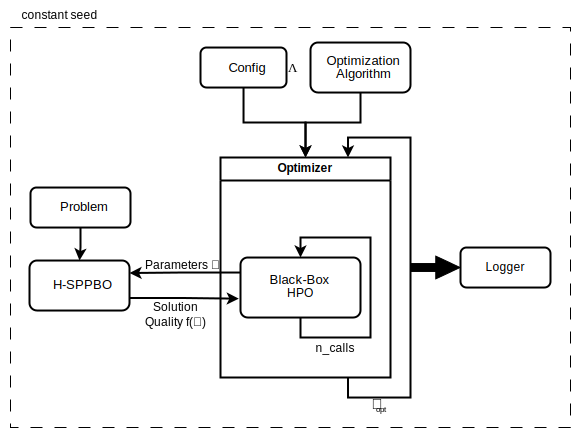
\includegraphics[width=0.8\textwidth]{optimizer_flow.svg}
	\caption{Visualization of the optimizer mode workflow.}
	\label{fig:optimizer-flow}
\end{figure}

\subsection{Experimentation Mode}
\label{chap:exp-mode}

The main task of the experimentation mode is to repeat multiple runs of a fixed metaheuristic, i.e. using only one parameter configuration. It is essentially a version of the run mode with options for multiple runs. Therefore, the inputs of this mode are also similar, with the parameter configuration $\mathbf{\lambda}$, problem parameters ($t, p, w_{di}$) and, additionally, the number of consecutive runs $r_\text{exp}$. The results for this mode are also logged in an averaged version, to easily plot the mean development of an algorithm across different random influences. For this reason, the random seed is not explicitly set to a fixed value in this mode. See \cref{alg:xf-opt-run-exp} for an implementation template.


\begin{algorithm}
	\caption{XF-OPT/HSPPBO: Experimentation Mode}
	\label{alg:xf-opt-run-exp}
	\begin{algorithmic}
		\Require Number of runs $r_{\text{exp}}$, parameter configuration $\mathbf{\lambda}$, problem parameters ($t, p, w_{di}$)
		\State $\mathbb{L}  \gets $ \Call{InitLogger}{ } 
		\State $\mathcal{P}  \gets $ \Call{InitProblem}{$t,p,w_{di}$}
		\State $\mathcal{M}  \gets $ \Call{InitHSPPBO}{$\mathcal{P}, \mathbb{L}, \mathbf{\lambda}$}
		\For{$i=1$ to $r_{\text{exp}}$}
			\State $\mathbf{s} \gets $ \Call{Execute}{$\mathcal{M}, \mathcal{P}$}
			\State \Call{LogResults}{$\mathbb{L}, \mathbf{s}$}
		\EndFor
	\end{algorithmic}
\end{algorithm}





% !TeX root = main.tex
% !TeX spellcheck = en-US
% !TeX encoding = utf8


\chapter{Experimental Design and Tests}
\label{chap:experiment}

\section{Choice of Problem Instances}
\label{chap:problem-choice}

This thesis builds on the foundation of the \glsfirst{hsppbo} work of \citet{kupfer2021hierarchical}. Therefore, the problem category was chosen analogously to the symmetric \glsfirst{tsp}. In this way, we can refer to previous work, while also generalizing many different, relevant problems (see \cref{chap:tsp}). 
The \gls{tsp} instance test cases were taken from the popular \textit{TSPLIB} benchmarking suite \cite{reinelt1991tsplib}, since they have been tried and tested in many publications and also have the advantage that the optimal solution is known for each of the problems, which enables further comparison with other metaheuristics. Besides the standard 2D Euclidean weights, there are also instances of geographic distance problems or distance matrices. The thesis focuses on 2D Euclidean instances for simplicity, but the software itself can handle most types of TSP edge weights (see \cref{chap:tsp-module}).

The thesis also aims at solving the \glsfirst{dtsp}. However, the dynamic part is implemented by the \texttt{problem} module itself, and is not a standard part of the \textit{TSPLIB} library. All \textit{TSPLIB} instances have a different number of cities $n$ (called dimension in the following), and often certain characteristics by which the cities are placed in their space, sometimes described in the \textit{TSPLIB} file (under \texttt{COMMENT}). An example of such a file is shown in \cref{lst:tsp-file}. To quantify these cases, several statistical values have been calculated for the corresponding distance matrices. These provide a way to select a meaningful, disjoint subset of problem instances without using too many, since the computational cost of running the larger instances can be quite significant.

\begin{Listing}
	\begin{minted}{text}
		
NAME : bier127
COMMENT : 127 Biergaerten in Augsburg (Juenger/Reinelt)
TYPE : TSP
DIMENSION : 127
EDGE_WEIGHT_TYPE : EUC_2D
NODE_COORD_SECTION
1   9860  14152
2   9396  14616
[...]
127   3248  14152
EOF
	\end{minted}
	\caption{The \textit{TSPLIB} file for the \texttt{bier127} problem instance (node list shortened).}
	\label{lst:tsp-file}
\end{Listing}


The selection of problem instances was influenced by two metrics: dimension $n$ and city placement characteristics. Since this implementation of the \gls{hsppbo} algorithm scales linearly with $n$, and the \glsfirst{hpo} process runs the algorithm multiple times (\texttt{n\_calls}), with the optimization also being repeated multiple times ($r_\text{opt}$) for each dynamic configuration and problem instance $\mathcal{P}$, the maximum dimension used is 450 to keep the computation time within a reasonable limit. The lower bound for the dimension $n$ is 50, since smaller instances make it difficult to detect any placement characteristics. This results in a dimension bounded by the interval $[50,450]$, which is then roughly divided into smaller instances (50-250 cities) and larger instances (250-450).

With the dimension partitioned, we are left with the statistical measures to analyze the placement characteristic. These measures have been chosen for their expressiveness in graph and distribution problems. Furthermore, it should be possible to calculate them as fast as possible. In order to justify the final choice of \gls{tsp} instances, various literature was searched for similar procedures.
Under the assumption that similarly structured \gls{tsp} instances share common parameter values for their metaheuristic solvers, the following problem classification aims to be very thorough, so that all parameters obtained for the smaller instances can later be used for the larger instances as well.

\subsection{Statistical Measures for Analysis}
\label{chap:prob-stat-meas}

The city placement characteristic was determined using the following statistical values, which was computed for each \textit{TSPLIB} instance over the corresponding distance matrix $D$ using the \textit{NumPy} package \cite{harris2020array}:

\begin{itemize}
	\item The mean $\mu$, median $\tilde{d}$ and standard deviation $\sigma$
	\item The coefficient of variation $c_\text{v}$
	\item The coefficient of quartile variation (CQV)
	\item The regularity index $R$
	\item The first eigenvalue $\lambda_1$
	\item The \enquote{eigen gap} $\Delta\lambda_{1,2}$, i.e. the gap between the first two eigenvalues
\end{itemize}

The mean, median, and standard deviation are common choices for analyzing data sets. These three values  already make it possible to give a first impression of how evenly the city nodes are distributed in Euclidean space. For example, if the mean distance between nodes differs greatly from the median with a high standard deviation, we can assume that the instance is somewhat unevenly distributed. However, since these values are absolute and therefore dependent on the problem and its distance scaling, they cannot be used for comparison across all instances.
Since we want to identify distributions and clusters within the \gls{tsp} instances, measures of statistical dispersion were preferred for further calculations. These provide insight into how compressed or stretched out a data set is. Furthermore, only dimensionless metrics were considered.

One possible measure of dispersion is the coefficient of variation, which improves on the standard deviation by effectively normalizing it by division with the mean: $c_\text{v} = \frac{\sigma}{\mu}$. This results in a relative value that can be used comparatively. However, the coefficient of variation tends to overexpose outliers, which may be undesirable when classifying highly clustered instances.
Another measure is the \gls{cqv}, which is a robust version of the coefficient of variation and therefore less sensitive to outliers \cite{bonett2006confidence}. It is defined as $CQV = \frac{Q_3 - Q_1}{Q_3 + Q_1}$, where $Q_1$ and $Q_3$ are the first and third quartiles of the distance matrices distribution.

The regularity index $R$ is a metric that was developed especially for the quantification of spatial distributions by \citet{clark1954distance}. It is defined as the ratio between the median distance between each nearest neighbor $r_A$ and the median distance between nearest neighbors under the assumption of a perfect random distribution $r_E$, specified by a density $\rho$, so that $R = r_A / r_E$.
Thus, a value of $R = 1$ would indicate a completely random distribution, while $R = 0$ would suggest that all nodes are located at the same position.
In order to compute this measure effectively, some considerations had to be made.
The numerator $r_A$ is easily calculated by using the minimum function over all possible distances for each node \cite{dry2012clustering}: 
\begin{equation}
	r_A = \frac{1}{n} \sum_{i \neq j}^{n} \min(d_{ij})
\end{equation}
In this case, however, the distance under random distribution depends on the area $A$ and the number of nodes $n$, with a point density of $\delta = n/A$. The formula for $r_E$ is described by a Poisson process for complete spatial randomness. By making some adjustments to incorporate a sense of absolute distance and taking the expectation of the resulting probability distribution, we get the following formula \cite{dry2012clustering}:
\begin{equation}
	r_E = \frac{1}{2} \sqrt{\frac{A}{n}}
\end{equation}
The area $A$ covered by the nodes, i.e. the convex hull of the graph, was obtained using the \textit{SciPy} library \cite{2020SciPy-NMeth}, which provides algorithms for scientific computing in \textit{Python}.
Although not originally applied to the \gls{tsp}, the works of \citet{dry2012clustering, cricsan2021randomness} give an insight into the suitability of the regularity index for this problem category, concluding that it is highly significant, even if not perfect. Finally, in an application of the research around spectral analysis of graph problems and the \gls{tsp}, the first two (largest) eigenvalues were computed over the distance matrix $D$. While the first eigenvalue can be related to average length of the Hamilton cycle in a \gls{tsp} instance \cite{cvetkovic2018traveling}, the \enquote{gap} between the first two eigenvalues could be used as a measure of connectivity \cite{lovasz20071}.

To have a larger sample set, all of these values were calculated for all \textit{TSPLIB} instances with a dimension less than 1000 and a valid edge weight type for the \gls{xfopt} package. This excluded \textit{ATT}, \textit{EXPLICIT}, and \textit{CEIL\_2D} problems, but included \textit{GEO} and \textit{ATT}, which resulted in metadata for 118 problem instances.

\subsection{Classification}
\label{chap:classification}

Using these statistical measures, three different methods were employed to classify these 118 \gls{tsp} instances. Since these statistics, except for the regularity index $R$, do not provide qualitative information about the type of class the instance belongs to, all of the graphs were also visualized using the \textit{NetworkX} package. This made it possible to interpret the resulting problem groups by formulating the similarities suggested by the classification. The exploration and application of each of these methods has yielded mixed results, with one clear winner.

\subsubsection{Method I - Regularity Index}

The first method is to use certain value ranges of the regularity index $R$ to discriminate between structures. As mentioned above, this procedure and the applicable ranges have already been validated for the application to the \gls{tsp} by previous work. To further replicate the results obtained by \citet{dry2012clustering, cricsan2021randomness}, additional \gls{tsp} instances from the University of Bonn's \textit{Tnm} test data set \cite{hougardy2021hard} and a triangle lattice generated using the aforementioned \textit{NetworkX} package were used. The implementation of this thesis was able to successfully reproduce the $R$ values from both papers, i.e., all the same values for the \textit{Tnm} \gls{tsp} and a value of $R = 2$, for a highly regular, uniformly distributed triangle lattice \cite{dry2012clustering}.
With this foundation established, the first method was applied to the selected \gls{tsp} instances using the following groups and their ranges:
\begin{itemize}
	\item Heavy clusters:	$R < 0.3$
	\item Semi-clustered: $0.3 \leq R < 0.8$
	\item Random Distribution: $0.8 \leq R < 1.2$
	\item Semi-regular: $1.2 \leq R < 1.4$
	\item Regular: $1.4 \leq R$
\end{itemize}
This first method generally worked well and was able to classify each problem into a satisfactory group. However, it was heavily influenced by higher dimensions and artificial patterns, such as with \textit{pcb442} or \textit{ts225} (see \cref{fig:pcb442,fig:ts225} for visualizations), where artificial is meant to describe that the placement of the cities is clearly influenced by a pattern. These instances were almost all incorrectly classified as randomly distributed ($R\approx1$). 
This method alone would not be able to reliably and disjunctively classify the instances.

\subsubsection{Method II - Eigenvalues of the Distance Matrix}

The second method, inspired by \citet{lovasz20071}, of using the gap between the first two eigenvalues of the distance matrix $D$ proved to be impractical to implement, since it could not be calculated directly on the distance matrix, and would instead use its Laplacian, which is computationally infeasible, especially for larger instances. The paper also states its theory on a positive semi-definite matrix, which the distance matrices used here are not. However, applying the \gls{tsp}-related approach of \citet{cvetkovic2018traveling} of using only the first eigenvalue as a classifier for Hamiltonian path length yielded interesting results. While most of the resulting eigenvalue groups were very unsatisfactory, there was one group consisting of all the artificially structured \gls{tsp} instances. Therefore, a combination of the two methods was the logical next step.

\subsubsection{Method III - k-means Clustering }

The first two methods already identified the regularity index and the first eigenvalue as expressive metrics for classification. With the \glsfirst{cqv} as an additional robust measure of dispersion, a successful classification should be possible. However, it is not practical to manually apply value ranges to three metrics. Therefore, a cluster analysis was performed using the k-means algorithm. 

The problem description for the k-means algorithm is given for a set of data points $n$ in $\mathbb{R}^d$. Given a variable number of $k$ centers, select the position of each center that minimizes the total squared distance from each point to its nearest center \cite{arthur2006k}. This NP-hard problem was originally solved by \citet{lloyd1982least}, resulting in \enquote{Lloyd's algorithm}, or \enquote{Voronoi iteration}. It randomly places $k$ centers in Euclidean space and assigns each point to its nearest center. It then computes a Voronoi diagram over the $k$ sites, integrates these cells, and moves the center to the centroid of each cell. This process is repeated until a stagnation condition is registered. The algorithm used for our application is called \textit{k-means++} and is based on this foundation. Instead of opting for an exact solution, \citet{arthur2006k} propose an approximate procedure to compute the initial $k$ centers. This way, fewer iterations of the otherwise same algorithm are needed to achieve converging behavior and thus satisfactory clusters. 

\begin{figure}
	\centering
	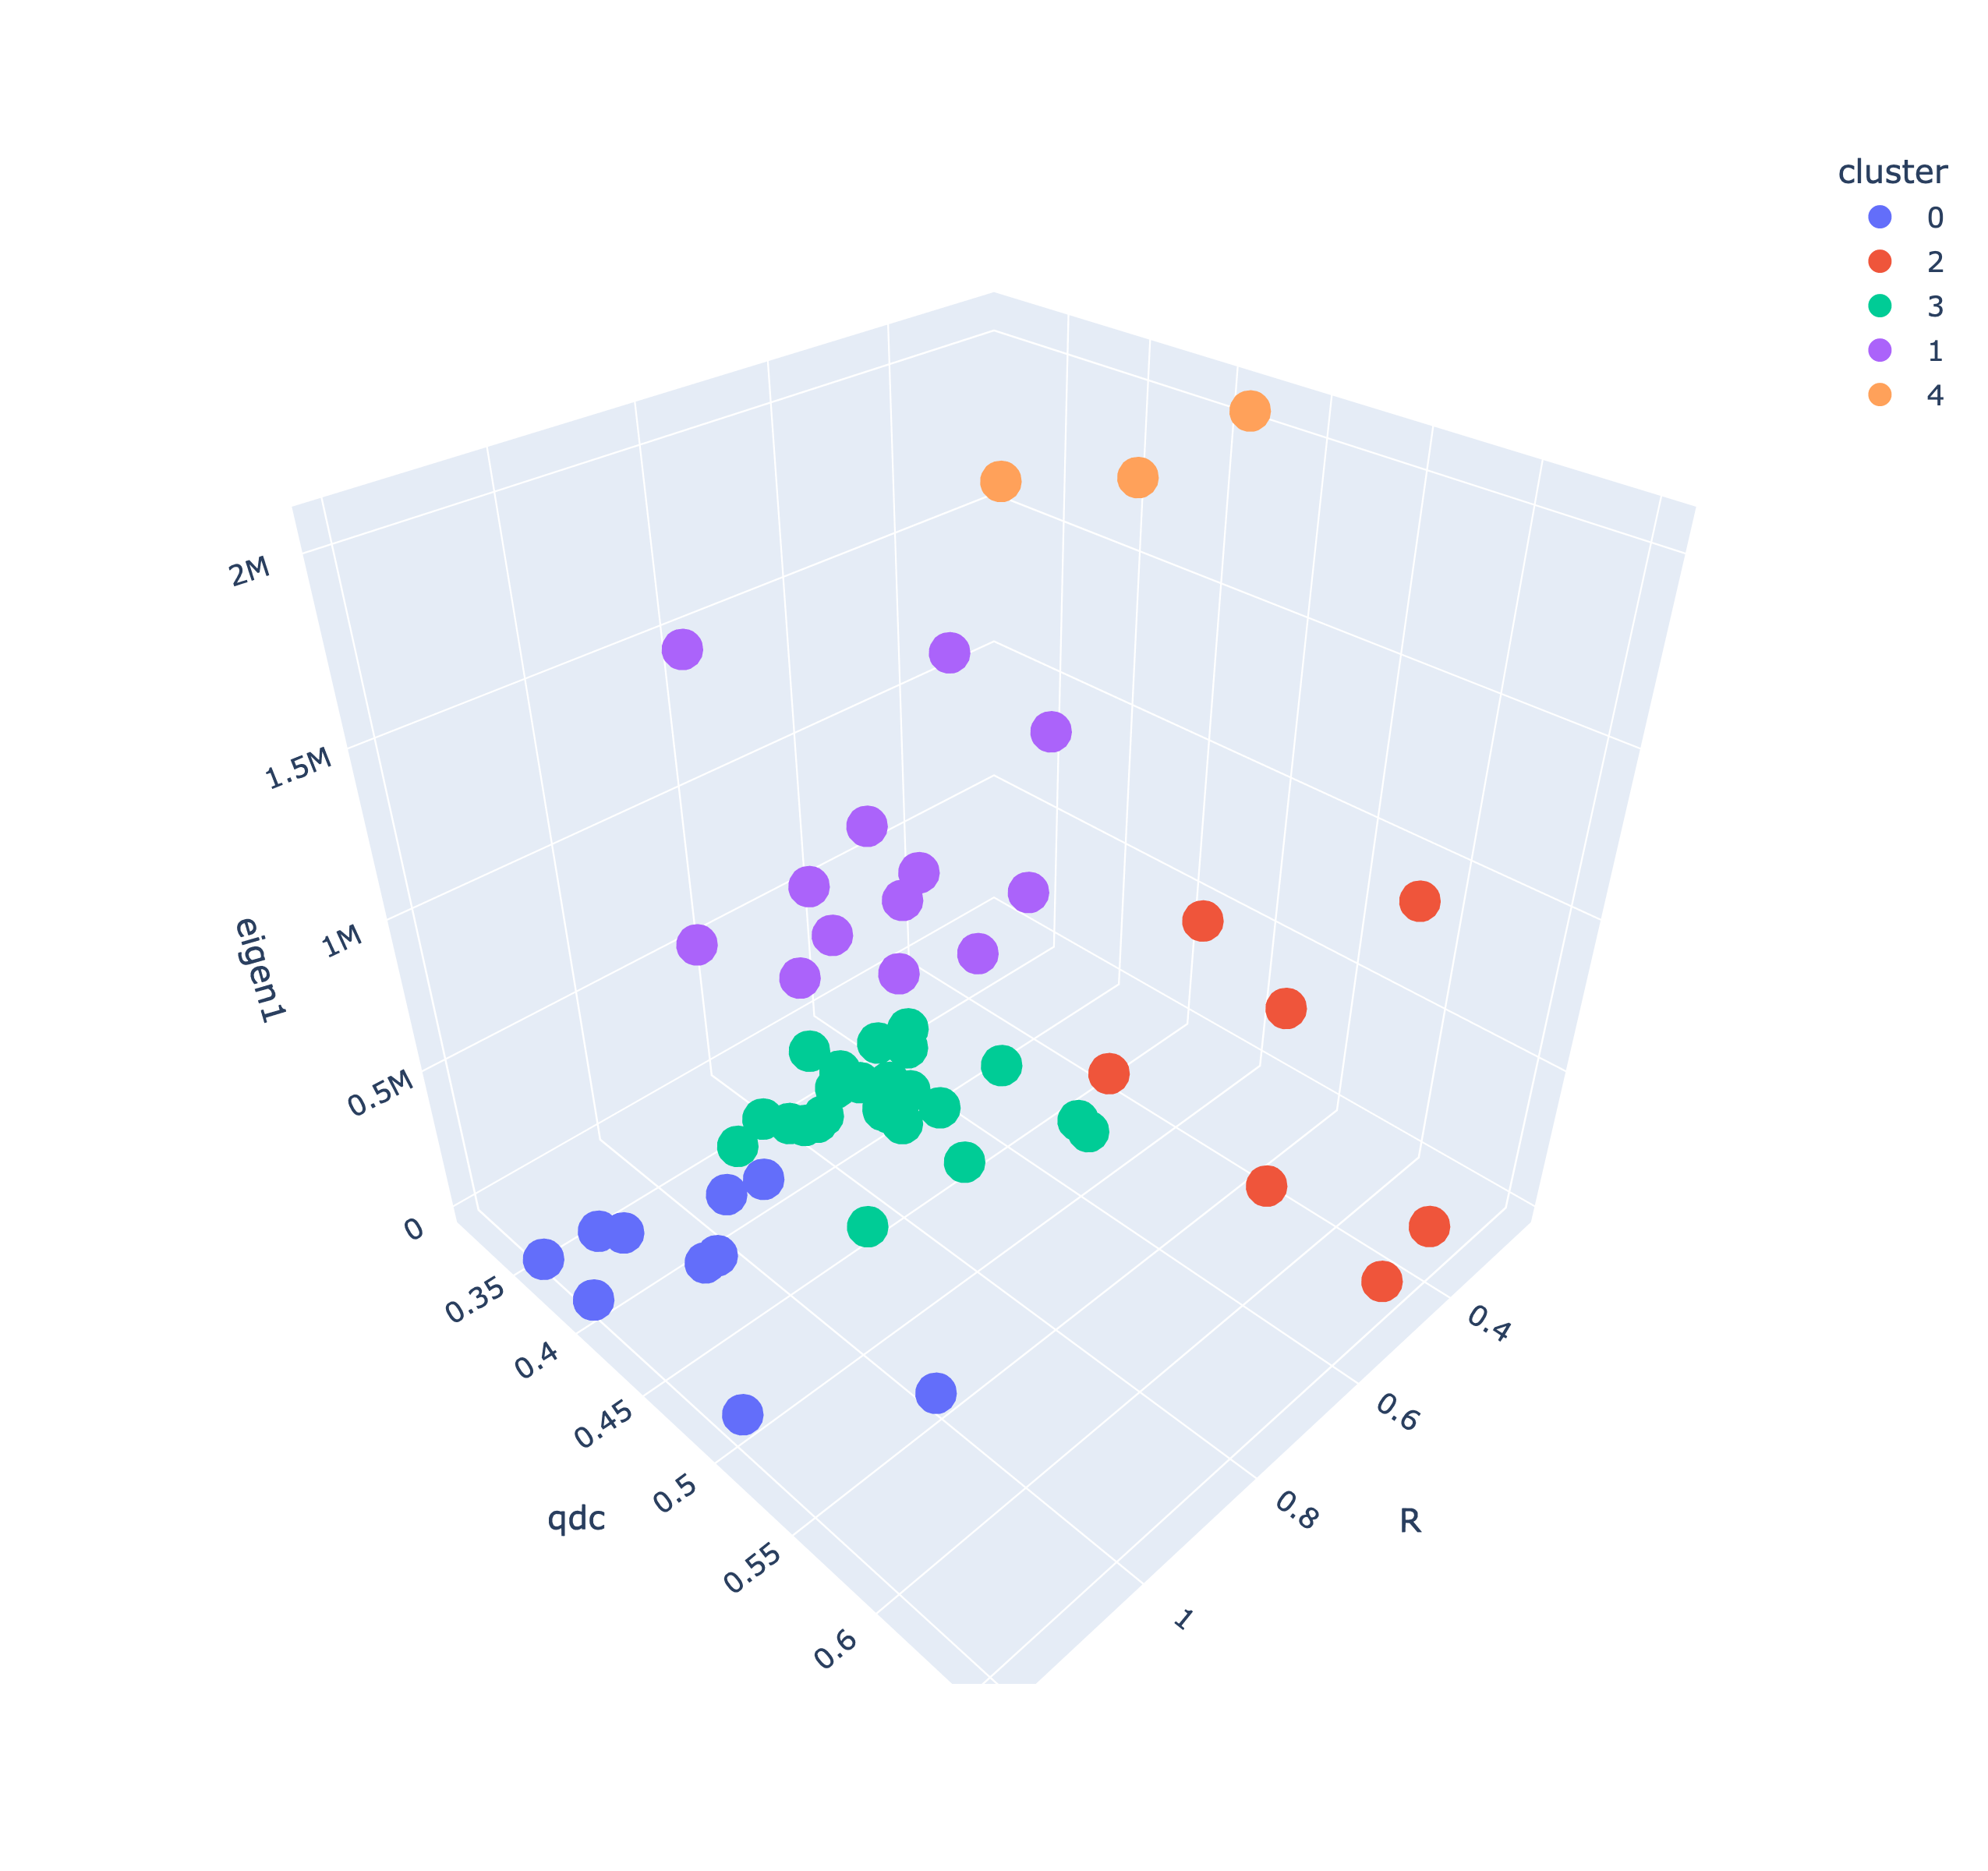
\includegraphics[width=0.9\textwidth]{clusters_kmeans.png}
	\caption[Visualization of the k-means cluster analysis]{Visualization of the k-means cluster analysis applied to 118 \gls{tsp} instances using $k=5$ clusters. Each data point is an instance placed into three-dimensional space using its regularity index $R$, its first eigenvalue (eigen1), and its \glsfirst{cqv}.}
	\label{fig:clusters-kmeans}
\end{figure}

The \textit{k-means++} algorithm was applied to all of the 118 instances, with the first eigenvalue $\lambda_1$, the regularity index $R$, and the \glsfirst{cqv} creating a three-dimensional real Euclidean space within these instances were places. Furthermore, a value of $k = 5$ clusters proved to be the most effective, since it corresponds to the groups mentioned in the first method and results in the most visually verifiable coherence between instances. As shown in the 3D scatter plot of the clustering in \cref{fig:clusters-kmeans}, this third method resulted in fairly consistent clusters and even managed to separate most of the artificial patterns from the rest, especially by using the eigenvalue. However, due to the nature of k-means clustering, there are no resulting structural properties attached to the generated clusters. We can only infer the structural properties mentioned above by looking at the ranges and visualizations for the clustered instances.
 
 The separation between instances shown in the scatter plot is fairly profound, with only the red and orange clusters looking a bit loosely connected. Nevertheless, the third method is convincing in most respects, making it an improvement over the mere value ranges of the first two methods. Therefore, the results of the clustering method are used to categorize the structure of the problem instances. To do this, the clustered groups must first be related to a structural property, as explained above. This is done by examining the value ranges of regularity index, as in the first method, the first eigenvalue, and by looking at the visualized instances to discover common patterns or to verify the implications of $R$ or the \gls{cqv} value. The resulting structural groups and their distinctive value ranges are as follows:
 
 \begin{enumerate}
 	\item Random to nearly regular distribution: $R > 0.9$
 	\item Smaller, slightly clustered areas with otherwise random structure: $R \in [0.55, 0.9]$ and $\lambda_1 < 500 000$
 	\item Artificially structured with certain patterns of medium clustered regions, with small distinct holes within the distribution: $R \in [0.55, 0.9]$ and $\lambda_1 > 500 000$
 	\item A few highly clustered areas: $\lambda_1 > 1 700 000$
 	\item Dispersed and highly clustered areas with few or no city nodes in between: $R < 0.6$ and $CQV > 0.5$ \end{enumerate}

The first, second, and fourth groups are very consistent, with only a few outliers present. The other two groups, three and five, consist of intermediate structures that could not be placed in any other group, but are also too different from each other, to justify only one group. 

With this classification in mind, 10 instances from each structural group with a smaller and a larger instance were selected for the thesis. The dimension limitation already excluded many instances, which made some choices very obvious. For example, the first group has no instance with a size between 250 and 450 nodes. So the next largest instance, \texttt{rat195}, was chosen as a replacement. Other groups had only a few possible candidates for each dimension class, so they were chosen randomly. The selected instances are the following, where the enumeration is coherent with the stated structural groups:
\begin{enumerate}
	\item eil51, rat195
	\item berlin52, gil262
	\item pr136, lin318
	\item pr226, pr439
	\item d198, fl417
\end{enumerate}
\Cref{fig:cluster-groups} shows the visualizations of these 10 instances, where each row of figures depicting a cluster group from 1 (top) to 5 (bottom), with the left column depicting smaller instances, and the right column depicting larger instances. Each figure is labeled with its instance name.

\begin{figure}[h!]
	\captionsetup[subfigure]{aboveskip=-1pt,belowskip=2pt}
	\centering
	\begin{subfigure}{0.3\textwidth}
		\centering
		\fbox{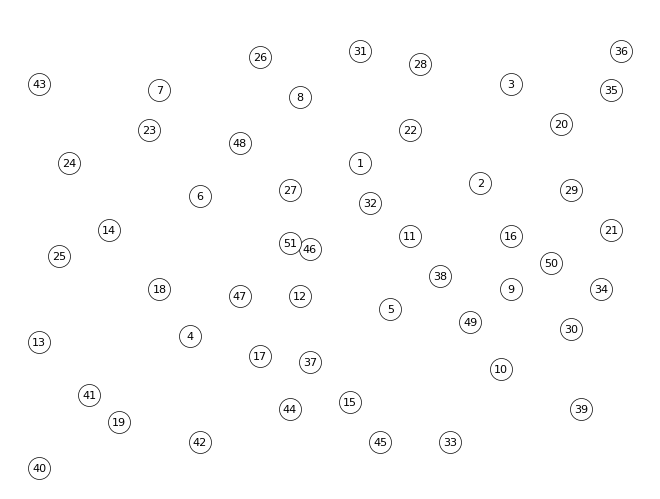
\includegraphics[width=0.85\columnwidth]{eil51.png}}
		\caption{eil51}
		\label{fig:eil51}
	\end{subfigure} 
	\begin{subfigure}{0.3\textwidth}
		\centering
		\fbox{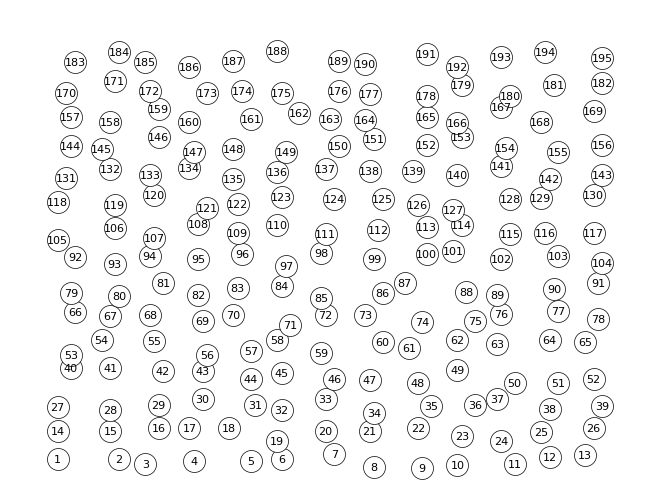
\includegraphics[width=0.85\columnwidth]{rat195.png}}
		\caption{rat195}
		\label{fig:rat195}
	\end{subfigure}

	\begin{subfigure}{0.3\textwidth}
		\centering
		\fbox{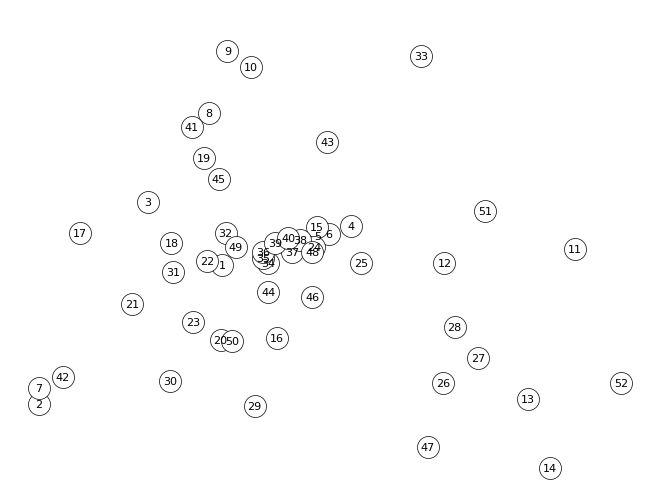
\includegraphics[width=0.85\columnwidth]{berlin52.png}}
		\caption{berlin52}
		\label{fig:berlin52}
	\end{subfigure} 
	\begin{subfigure}{0.3\textwidth}
		\centering
		\fbox{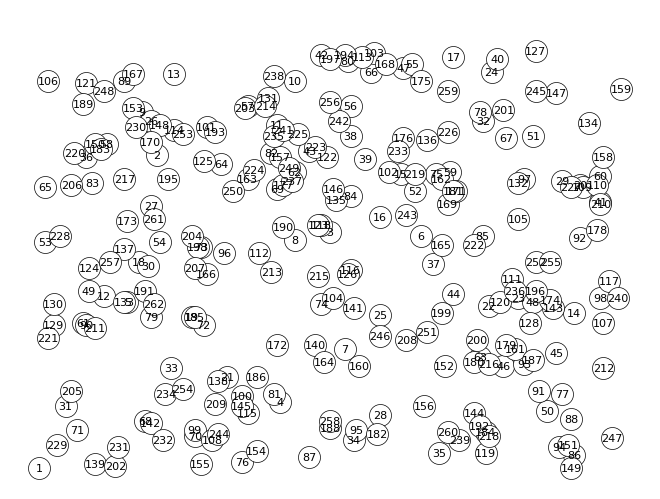
\includegraphics[width=0.85\columnwidth]{gil262.png}}
		\caption{gil262}
		\label{fig:gil262}
	\end{subfigure}

	\begin{subfigure}{0.3\textwidth}
		\centering
		\fbox{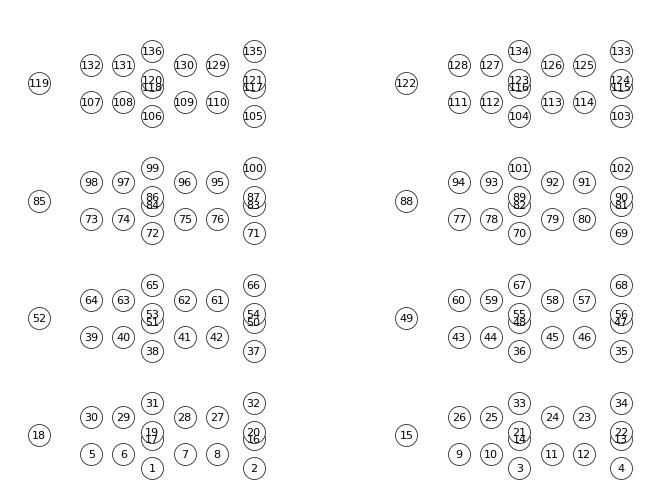
\includegraphics[width=0.85\columnwidth]{pr136.png}}
		\caption{pr136}
		\label{fig:pr136}
	\end{subfigure} 
	\begin{subfigure}{0.3\textwidth}
		\centering
		\fbox{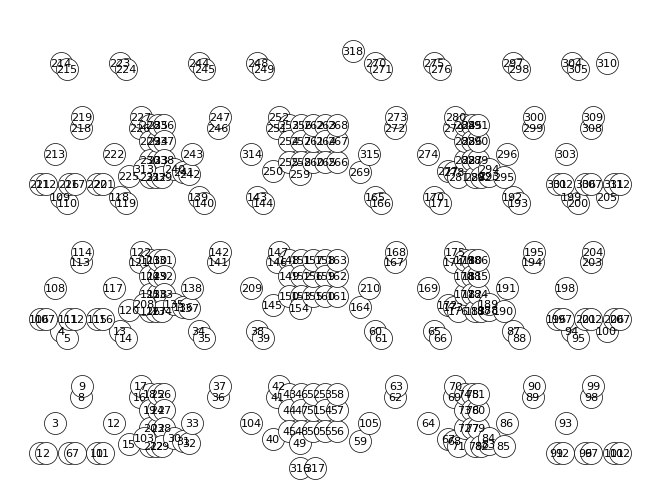
\includegraphics[width=0.85\columnwidth]{lin318.png}}
		\caption{lin318}
		\label{fig:lin318}
	\end{subfigure}

	\begin{subfigure}{0.3\textwidth}
		\centering
		\fbox{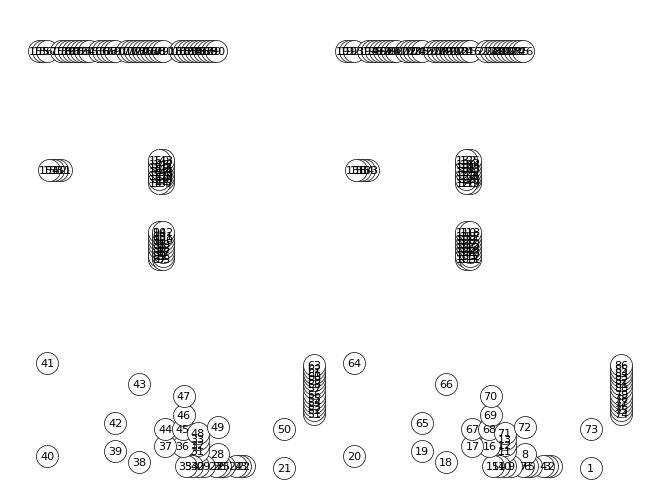
\includegraphics[width=0.85\columnwidth]{pr226.png}}
		\caption{pr226}
		\label{fig:pr226}
	\end{subfigure} 
	\begin{subfigure}{0.3\textwidth}
		\centering
		\fbox{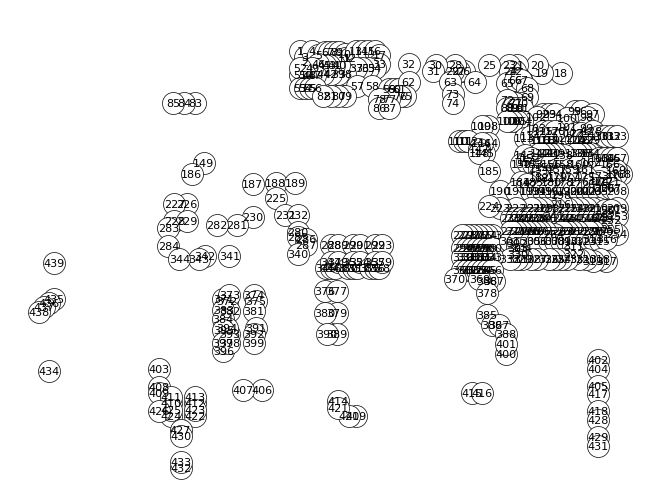
\includegraphics[width=0.85\columnwidth]{pr439.png}}
		\caption{pr439}
		\label{fig:pr439}
	\end{subfigure}

	\begin{subfigure}{0.3\textwidth}
		\centering
		\fbox{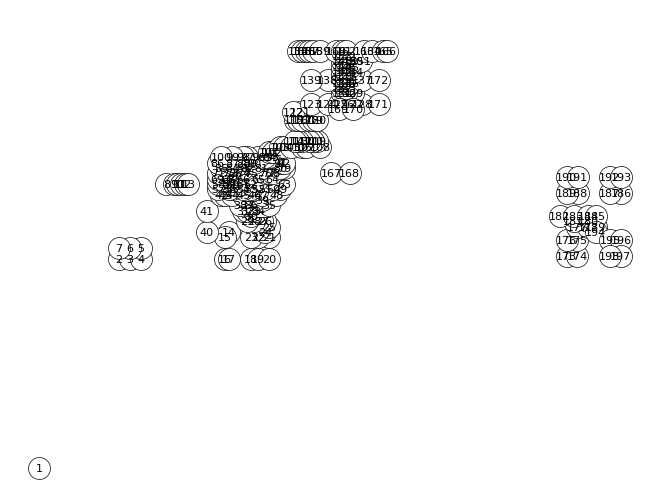
\includegraphics[width=0.85\columnwidth]{d198.png}}
		\caption{d198}
		\label{fig:d198}
	\end{subfigure} 
	\begin{subfigure}{0.3\textwidth}
		\centering
		\fbox{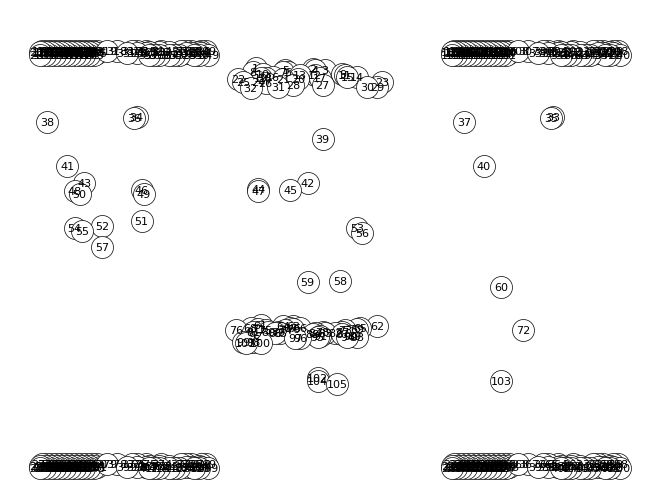
\includegraphics[width=0.85\columnwidth]{fl417.png}}
		\caption{fl417}
		\label{fig:fl417}
	\end{subfigure}

	\caption[Visualizations of the \gls{tsp} instances used in the experiments]{Visualizations of the \gls{tsp} instances used in the experiments. Each row of figures is a cluster group, where the left column depicting smaller instances and the right column depicting larger instances. Each figure is labeled with its instance name.}
	\label{fig:cluster-groups}
\end{figure}

\section{Choice of Optimization Methods}
\label{chap:opt-choice}

The choice of \gls{hpo} pipelines (i.e., acquisition function + surrogate model) to be tested was largely dictated by the \gls{ml} library chosen, \texttt{scikit-optimize}. This is due to the fact that there is very little research on applying \glsdesc{hpo} to the tuning problem of metaheuristics. The only relevant work found was by \citet{yin2021bayesian}, who have a very similar application, using \gls{hpo} to tune an \glsdesc{aco} algorithm. However, they focus only on \gls{bo} using \gls{gp} as a surrogate model. Furthermore, it was noticed that many \gls{ml}-related explanations of \gls{bo} ignore the fact that the surrogate model can even be changed. Thus, in addition to the originally proposed choice of a \glsdesc{gp}, regression models from the field of ensemble learning were also used. Although both \glsdesc{rf} and \glsdesc{gbrt} are based on decision trees, they differ greatly in the way they use their basic learners for the ensemble predictor (averaging vs. boosting). Therefore, they cover a large part of state-of-the-art ensemble methods.

As already described in \cref{chap:optimizer}, the following surrogate models are provided: \glsfirst{rf}, \glsfirst{gp}, \glsfirst{rf}, \glsfirst{et}, and \glsfirst{gbrt}.
All of these models were used in the experiments, with the exception of the standard \gls{rf}, since \gls{et} already improves on it. This range of models should ensure that as many optimization scenarios as possible can be tested to find the ideal method for metaheuristics, or at least the \gls{hsppbo} algorithm. In addition, \gls{rs} was also used and provides a good baseline, since it is a model-free method and therefore makes no assumptions about the objective function. However, the choice of acquisition function was made with respect to the surrogate model used. The following subsection describes how the \gls{bo} process was initialized for each method.

\subsection{Optimizer Initialization}
\label{chap:opt-init}
The initialization process can have a large effect on the outcome of the \gls{hpo} process. For all methods, a set of 10 starting points ($\mathcal{D}_\text{init}$) has been sampled using a specified method before the acquisition function was utilized for sampling, which is the default value of the library. The \gls{rs} algorithm has only this sampling method as a possible initialization metric. Besides the default uniform random number generator, there are several low-discrepancy sequences, such as the Hammersely sequence, and a Latin hypercube sampling method to choose from. Since we want to use \gls{rs} as a baseline in later discussion, the default uniform sampling was used.

As mentioned above, the work of \citet{yin2021bayesian} was a useful starting point for the \gls{gp} surrogate model. They tried out different initializations for the \gls{bo}, including all three acquisition functions (\gls{pi}, \gls{ei}, \gls{lcb}), initial sampling methods, noise functions and values for improvement $\xi$. After reviewing their results, the most appropriate values were used to initialize the \gls{gp} model used in the thesis. The acquisition function was selected as \glsfirst{pi} with an improvement rate of $\xi = 0.01$, because it shows fast convergence behavior with good results. The kernel function was selected as a Matérn kernel with $\upsilon=5/2$, which is the default of the \texttt{scikit-optimize} library. It also uses an additive white noise kernel to account for a noisy objective function. However, instead of the default Gaussian noise scaled by the variance during the optimization process (see \cref{eq:gauss-noies}), a white noise kernel with a constant variance of 0.7 was chosen, to prevent bad search areas from gaining too much relevance for sampling \cite{yin2021bayesian}.
Furthermore, a low-discrepancy Hammersely sequence was chosen over the default uniform distribution for initial sampling, as the \gls{gs} model appears to benefit from more evenly spaced out points \cite{cervellera2013learning}. 

No evidence was found to apply this reasoning to the other two models, \gls{et} and \gls{gbrt}, so instead, they use the standard uniform sampling and the default \gls{ei} acquisition function with $\xi = 0.01$ suggested by the library. Also, no additional noise was added to the methods. The initialization values for each estimator are summarized in \cref{tab:opt-init}.

\begin{table}
	\centering
	 \caption[The \gls{hpo} methods used and their initialization values]{The \gls{hpo} methods used and their initialization values.}
	\label{tab:opt-init}
	\begin{tabular}{c|c|c|c}
		Estimator & Acquisition Function & Sampling Method & Number of initial points $\mathcal{D}_\text{init}$ \\
		\hline
		\gls{rs} & - & Uniform & -\\
		\gls{bo}-\gls{gp} & \gls{pi} ($\xi=0.01$) & Hammersley & 10 \\
		\gls{bo}-\gls{et} & \gls{ei} ($\xi=0.01$) & Uniform & 10 \\
		\gls{bo}-\gls{gbrt} & \gls{ei} ($\xi=0.01$) & Uniform & 10 \\
	\end{tabular}
\end{table}

As explained in \cref{chap:opt-mode}, the random seed of each method was set according to the current iteration of the optimization run. This ensures new samples and results for each optimization run, while also providing reproducibility.

\section{Choice of Parameters and Value Ranges}
\label{chap:choice-param}

Since the focus of this thesis is on finding ideal parameter combinations using \gls{ml}-based \glsdesc{hpo} algorithms, we do not need to specify exactly which parameter values we want to test, as many other metaheuristics work does prior to experimentation. However, we still need to specify which of the available parameters of the \gls{hsppbo} algorithm we want to optimize automatically, if so, what range these parameters are sampled from during the process, and if not, what static parameter value we should assign and why.

In general, the parameter configuration space $\Lambda$ should be as broad as computationally feasible and logically useful to avoid unwanted effects like the \enquote{Floor and Ceiling effect} \cite[p.~47]{vogt2011dictionary}. Otherwise, it would impose certain expectations on the optimization process and its parameter choices, and it would also limit the potential for interesting new global optima. For example, although we can expect good results from $\beta = 5$, due to many other parameter influences, we cannot know for sure if a value of $\beta = 10$ might also be a good choice in some parameter combinations.

As already explained in \cref{chap:hsppbo-module}, the following are all the available parameters for the \gls{hsppbo} algorithm that qualify for optimization, their corresponding \gls{hpo} data type, and their default range:
\begin{itemize}
	\item $w_{\text{persprev}}, w_{\text{persbest}}, w_{\text{parentbest}} \geq 0$ (real)
	\item $\alpha, \beta \geq 0$ (integer)
	\item $\theta \in [0,1]$ (real)
	\item $H = \left\lbrace H_{\text{full}}, H_{\text{partial}}, \emptyset \right\rbrace$ (categorical)
	\item $0 < L_\text{pause} < 100$ (integer)
\end{itemize}

Unfortunately, these standard data ranges were too broad to use in the experiments. Therefore, parameter influences, effects, and existing justifications for limitations were investigated.
The parameters $H$ and $\theta$ are closely related to the hierarchical part of the \gls{hsppbo} algorithm, so there is almost no reference to existing implementations or papers, except for \citet{janson2006hierarchical} with their hierarchical version of a \glsfirst{pso} algorithm. Regarding the parameter $H$, \citet{kupfer2021hierarchical} found that the $H_{\text{partial}}$ response often outperforms the $H_{\text{full}}$ response, and the changing heuristic influence controlled by $\beta$ during the optimization runs suggests an interesting behavior of this parameter. Thus, both response types were used. To use this categorical value for all of the aforementioned surrogate models, a one-hot encoding was applied prior to the optimization process. It maps each categorical value to a bit vector containing only a single 1 and 0 otherwise. For example, a possible one-hot encoding for $H$ could be $01$ for $H_{\text{full}}$ and $10$ for $H_{\text{partial}}$.

The detection rate $\theta$ seems to benefit from values higher than 0.1, and gets mixed results from values between 0.25 and 0.5, depending strongly on the problem instance and its dynamic intensity $C$ \cite{kupfer2021hierarchical}. Since values higher than 0.5 would render the need for a change handling procedure obsolete because the changes would most certainly be undetected, a range of $\theta \in [0.1, 0.5]$ was tested. 

The $L_\text{pause}$ parameter is also related to this particular implementation of the algorithm's dynamic handling. Since its only purpose is to disable detection right after each change interval by the \gls{dtsp} instance, it only needs to be high enough to account for the rearrangement of the \gls{sce} tree. And since it introduces the risk of unfair prior knowledge of the dynamic interval, it should be as small as possible, since a value equal to the dynamic period $T_{d}$ would make it impossible for the algorithm to falsely detect a dynamic event. Considering the theoretical \enquote{worst case} behavior of a complete reorganization on all three levels of the ternary tree with $13$ \glspl{sce}, a value of $L = 5$, also used in \cite{kupfer2021hierarchical}, is very reasonable.

The values for $\alpha$ and $\beta$ are used in almost every \gls{aco} variant and many metaheuristics in general. Since the work of \cite{dorigo1996ant}, most papers on \gls{aco} variants use $\alpha$ and $\beta$ values between 0 and 5, often following the recommendation by Dorigo ($\alpha = 1, \beta = 5$). However, this only really applies to these \gls{aco} versions used on symmetric \gls{tsp} instances, while the \gls{hsppbo} algorithm combined with \gls{dtsp} instances behaves very differently. In addition, works such as \cite{stutzle2012parameter, tuani2018h, wong2008parameter} imply that good parameter combinations may differ greatly from the original recommendation depending on the problem type and algorithm, and have success using values of 10 or higher. Since $\alpha$ and $\beta$ are exponents, and the expression in which they are used (see \cref{eq:hsppbo_tau}) is normalized to a probability anyway, the values should be considered relative to each other rather than absolute. Therefore, they should be at least $10\%$ apart to cover any reasonable combination of the two. Larger value ranges would carry the risk of reducing the other parameter to a value where it loses its significance and is effectively deactivated, while this should be preferably achieved by choosing a value of 0. It could also be argued that, based on this logic, a real value chosen from $[0,1]$ would also result in similar expressiveness. However, natural numbers are most often used for these parameters, and make for a much easier comparison. This resulted in a range of $\alpha,\beta \in [0,10]$, with $\alpha,\beta \in \mathbb{N}$.

The three weights $w_{\text{persprev}}, w_{\text{persbest}}, w_{\text{parentbest}}$ present an interesting significance. Although they are specific to this algorithm, they are based on the work by \citet{lin2015simple}, which in turn is based on the standard pheromone evaporation coefficient $\rho$ used in the standard \glsdesc{aco} and its variants. This value, which acts as a weight, is often chosen as $\rho \in (0,1]$. In \cite{lin2015simple}, a global population is introduced into the algorithm, and the total weight is divided by the number of iterations $k$ for which the solution is retained, or by the number of solutions generated per iteration, always using a specific formula that does not allow the full range of real numbers to be chosen. They also tested several values for the total weight (up to $w_\text{total} = 192$) and the elite solution weight (up to $w_\text{elite} = 10$), and often found that higher values were beneficial to solution quality. However, these results were obtained with $\alpha$ set to 1 and $\beta$ set to 5. This may not be optimal, since the three weights are summed and then influenced by the control parameter $\alpha$, which then has to be compared with its factor, the heuristic part, and its control parameter $\beta$. This means that the summed base, which is the three weights plus a fixed random weight ($w_\text{rand}$), is directly compared to the base of the heuristic term, which is the inverse of an element of the distance matrix $1 / d_{ij}$ ($d_{ij} \in D$). This value should be less than 1 and greater than 0, at least for a non-normalized, Euclidean distance matrix over common TSP instances. Therefore, the sum of the weights should also be close to this range of values. This allows the parameters $\alpha$ and $\beta$ to control only the influence of their respective bases, and not also to serve as a normalization exponent to bring the factors to a comparable level.

Furthermore, being able to take each weight from the entire real space of $[0,1]$ ultimately has the same effect as having predefined formulas for each weight category that scale with a total weight as in \cite{lin2015simple}. If the term is scaled by an exponent anyway, a weight difference between $0.01$ and $1$ has the same influence as between 1 and 100. Finally, since the random weight is fixed to $w_\text{rand} = 1/(n-1)$, where $n$ is the dimension of the TSP instance, the other weights must be comparable to it. A theoretical minimum of $n = 2$ cities results in a random weight of 1, while a maximum weight cannot be formulated, but is always greater than 0. This all led to the three weights being drawn from the real interval $(0, 1)$. However, since the python package \texttt{scikit-optimize} can only use closed real intervals, and the largest data set has a size of 450, which results in $w_\text{rand} = 0.0022$, the interval $[0.001,0.99]$ was used.

To conclude, the final parameter ranges are as follows:
\begin{itemize}
	\item $w_{\text{persprev}}, w_{\text{persbest}}, w_{\text{parentbest}} \in [0.001,0.99]$
	\item $\alpha, \beta \in \left\lbrace x\in\mathbb{N} | 0 \leq x \leq 10 \right\rbrace$
	\item $\theta \in [0.1,0.5]$
	\item $H = \left\lbrace H_{\text{full}}, H_{\text{partial}} \right\rbrace$
	\item $L_\text{pause} = 5$ (not optimized)
	
\end{itemize}

\section{Testing Procedure}
\label{chap:testing}

The basis of each test was the \gls{hsppbo} algorithm implemented as explained in \cref{chap:implementation}, running $i_\text{max} = 2600$ iterations on a \gls{dtsp} instance, hereafter referred to as a \gls{hsppbo} execution. The dynamic part (swapping a percentage of cities) happened every $T_d = 100$ iterations, starting at iteration 2000. Therefore, a dynamic change was triggered every $2000 + k \cdot 100 < 2600, k \in \mathbb{N}$ iterations. In this context, an important change was made to the solution quality function, which returns the tour length at the end of each \gls{hsppbo} execution to the optimization process. Instead of reporting only the last solution, i.e. the global best solution at iteration $i_\text{max}$, which would effectively only evaluate the response to the last dynamic event between iterations 2500 and 2599, all solutions just before each next dynamic change are stored. This means that between iterations 1999 and 2599, a total of seven solutions are stored, which are computed to solution qualities (lengths) and then averaged, resulting in $\overline{L}$. Thus, we are not only able to evaluate the dynamic response for all six dynamic events, but can also include the solution quality of the static \gls{tsp} up to iteration 1999, albeit with a small weighting of $1/7$ in the average. The run and experimentation modes are not affected by this change.

Each of the 10 problem instances mentioned above was used with a varying dynamic intensity set to $C \in \left\lbrace 0.1,0.25,0.5\right\rbrace$. The experiments performed in this thesis can be divided into three main parts. First, optimization data was collected for all four \gls{hpo} methods. Second, multiple optimization runs of only the best performing \gls{hpo} algorithm were executed. And third, the best parameter sets from the previous test were used to repeat multiple experiment runs. An overview of these tests and their execution parameters is summarized in \cref{tab:exp-setup}. The details and rationale for each part are explained in the following. 

\begin{table}[ht]
	 \caption{The three experimentation parts and their execution parameters.}
	\label{tab:exp-setup}
	\centering
	\begin{adjustbox}{width=1\textwidth}
	\begin{tabular}{c c c c c c c}
		\hline
		\thead{Mode of\\Operation} & \thead{HPO Method} $\mathcal{A}$ & \thead{n\_calls} & \thead{runs\\ ($r_\text{opt}$/$r_\text{exp}$)} & \thead{Dynamic Intensity $C$} & \thead{Number of\\Instances} & \thead{\gls{hsppbo}\\Executions} \\
		\hline
		optimizer & \makecell{\gls{rs}, \gls{gp},\\ \gls{et}, \gls{gbrt}} & 30 & 3 & 0.25 & 5 (small) & 1800 \\

		optimizer & \gls{gbrt} & 60 & 6 & all & 5 (small) & 5400 \\
		experimentation & - & - & 20 & all & 10  & 2 x 600 \\ \hline
	\end{tabular}
\end{adjustbox}
\end{table}

The first part deals with the selection of the most appropriate \gls{hpo} method for the \gls{hsppbo} algorithm and its dynamic problem instances. For this purpose, three optimization runs were performed for each of the four optimization algorithms (\gls{rs}, \gls{gp}, \gls{et}, \gls{gbrt}) and selected the algorithm based on the highest average solution quality and convergence rate. Each of these runs made 30 calls to the \gls{hsppbo} algorithm (\texttt{n\_calls }$= 30$) on only the five smaller problem instances and only the medium dynamic intensity ($C = 0.25$). Thus, four optimization methods, each performing three optimizer runs with 30 objective calls per run, on five instances with one dynamic intensity. This resulted in a total of 1800 \gls{hsppbo} algorithm executions. Some shortcuts had to be taken in this step to save some execution time. Since a full evaluation of all three dynamic intensities would take too long, the test was limited to the smaller \gls{tsp} instances and the medium dynamic intensity of 0.25. Furthermore, the \gls{bo} process was limited to only 30 objective function calls instead of 50 or more, which means that a convergent behavior should have started after about 20 calls \cite{head2016}. This de facto requirement for fast convergence can also be seen as a demand on the \gls{hpo} method chosen. Finally, the stability or robustness of the parameters chosen by the optimizers is of only secondary importance in this part, so that three runs are sufficient for an average solution quality.

In the second part, multiple evaluations were performed using all three dynamic intensities, with the most appropriate optimization method selected from the previous part. These results give us insight into what the optimal parameter selection might be for each, or potentially all, problem instances. To do this, six optimizer runs $r_\text{opt}$ were executed using one optimization algorithm, each run making 60 objective calls (\texttt{n\_calls}) to the \gls{hsppbo} algorithm, again only on the five smaller problem instances, but on all three dynamic intensities $C \in \left\lbrace 0.1,0.25,0.5 \right\rbrace$ for a total of 5400 \gls{hsppbo} algorithm executions. As explained earlier, the larger instances were not used due to time constrains. However, to get a more robust sense of \enquote{good} parameter configurations, the number of optimization runs was increased to six.

The resulting data sets $\mathcal{D}$ of these first two experimentation parts can best be expressed by a four-dimensional tensor, with the dimensions being the \gls{hpo} method $\mathcal{A}$, the \gls{tsp} instance $p$, the dynamic intensity $C$ and the number of consecutive optimization runs $r_\text{opt}$. Each element of this tensor consists of an optimizer result, consisting of, among other things, the entire parameter history of this run $\mathcal{H}(\mathbf{\lambda}, f(\mathbf{\lambda}))$, the best parameter configuration found $\mathbf{\lambda^*}$, and the trained surrogate model $\mathcal{M}$. So each data entry can be characterized by the function $\mathcal{D}(\mathcal{A},p,C,r_\text{opt}) \to \left\lbrace \mathcal{H}(\mathbf{\lambda}, f(\mathbf{\lambda})), \mathbf{\lambda^*}, \mathcal{M} \right\rbrace $, where 	$\mathcal{D}^i_{\mathcal{A}_j,p_k,C_l} \in \mathcal{D}(\mathcal{A},p,C,r_\text{opt})$ and $1 \leq i  \leq r_\text{opt}$.

 However, since the first part only used only a single dynamic intensity $C$ and the second part used only a single \gls{hpo} method $\mathcal{A}$, each of the resulting data sets can be reduced to a 3D-tensor.
 \cref{fig:dataset-opt} shows a representation of this explanation for the second part and its data sets.

\begin{figure}
	\centering
		\begin{adjustbox}{width=0.7\textwidth}
			\begin{tikzpicture}[>=stealth]
				\begin{scope}[shift={(45:3)}]
					\node[matrixlayer=red] (m3){
						\mathcal{D}^1_{p_1,C_3} & \mathcal{D}^1_{p_2,C_3} & \mathcal{D}^1_{p_3,C_3} &\cdots \\
						\mathcal{D}^2_{p_1,C_3}  & \mathcal{D}^2_{p_2,C_3} & \mathcal{D}^2_{p_3,C_3}&\cdots \\
						\mathcal{D}^3_{p_1,C_3}  & \mathcal{D}^3_{p_2,C_3} & \mathcal{D}^3_{p_3,C_3}&\cdots \\
						\vdots&\vdots&\vdots&\ddots\\
					};
				\end{scope}
				\begin{scope}[shift={(45:1.5)}]
					\node[matrixlayer=teal] (m2){
						\mathcal{D}^1_{p_1,C_2} & \mathcal{D}^1_{p_2,C_2} & \mathcal{D}^1_{p_3,C_2} &\cdots \\
						\mathcal{D}^2_{p_1,C_2}  & \mathcal{D}^2_{p_2,C_2} & \mathcal{D}^2_{p_3,C_2}&\cdots \\
						\mathcal{D}^3_{p_1,C_2}  & \mathcal{D}^3_{p_2,C_2} & \mathcal{D}^3_{p_3,C_2}&\cdots \\
						\vdots&\vdots&\vdots&\ddots\\
					};
				\end{scope}
				
				\begin{scope}
					\node[matrixlayer=blue] (m1){
						\mathcal{D}^1_{p_1,C_1} & \mathcal{D}^1_{p_2,C_1} & \mathcal{D}^1_{p_3,C_1} &\cdots \\
						\mathcal{D}^2_{p_1,C_1}  & \mathcal{D}^2_{p_2,C_1} & \mathcal{D}^2_{p_3,C_1}&\cdots \\
						\mathcal{D}^3_{p_1,C_1}  & \mathcal{D}^3_{p_2,C_1} & \mathcal{D}^3_{p_3,C_1}&\cdots \\
						\vdots&\vdots&\vdots&\ddots\\
					};
				\end{scope}
				
				\begin{scope}[->,thick]
					\draw ([shift={(0,-.3)}]m1.south west)--([shift={(0,-.3)}]m1.south east) node[midway,below]{instance $p$};
					\draw ([shift={(.5,0)}]m1.south east)--([shift={(.5,0)}]m3.south east) node[midway,rotate=45,below]{dynamic intensity $C$};
					\draw ([shift={(-.3,0)}]m1.north west)--([shift={(-.3,0)}]m1.south west) node[midway,rotate=90,above]{optimization run $r_\text{opt}$};
				\end{scope}
			\end{tikzpicture}
		\end{adjustbox}
	\caption{3D tensor representation of the data set $\mathcal{D}_{\mathcal{A}=\gls{gbrt}}(p,C,r_\text{opt})$ of the second experimentation part.}
\label{fig:dataset-opt}
\end{figure}

After this second part, we had 15 sets of optimal parameters, one for each combination of problem category (five groups as explained in \cref{chap:classification}) and dynamic intensity ($C \in \left\lbrace 0.1,0.25,0.5\right\rbrace$). Although the inclination to aggregate these parameter configurations in some way (e.g., an average of all three dynamic intensities for each problem category) is tempting,  not only because it would simplify the next part, but also because it would provide a multipurpose parameter recommendation, it was omitted for several reasons. First, it introduces a whole new perspective to this work, namely how parameters can be generalized across different problem descriptions. However, the goal of this work, as explained in the  \nameref{chap:approach} subsection, was to directly apply \glsdesc{hpo} to metaheuristics and validate it as a viable option. Any generalization would compromise this goal and open up the research question to several new variables. Second, by looking at the results of the second part of the experiment, it was clear early on that there were huge differences between the optimization runs and each of their optimal parameter sets. Except perhaps for $\alpha$ and $\beta$, any aggregation of parameters would have been a mostly arbitrary choice, with a few exceptions. This circumstance is discussed further in \cref{chap:part2}.

The third and final part verifies the previously selected \enquote{optimal} parameter selection. These 15 parameter sets were tested on their respective problem instances and dynamic intensities, with 20 experimental runs $r_\text{exp}$ each using the experimentation mode (see \cref{chap:exp-mode}). This time, all 10 instances were used. Since the problem classification effort was also made to obtain coherent instance groups, these parameter sets acquired using the smaller instances were also applied to the larger instances of each group. Therefore, each of these 15 parameter sets is used two times, for a total of 30 different combinations of problem instance and dynamic. This results in 600 runs of the \gls{hsppbo} algorithm.
As a reference for how well these \gls{hpo} parameter configurations perform, a general purpose parameter set (see \cref{tab:part3-gen-params}) was also applied to all 10 instances with all three dynamic intensities, again repeating each experimental run 20 times, yielding another 600 \gls{hsppbo} algorithm executions.
The values for $\alpha, \beta, w_{\text{persprev}}, w_{\text{persbest}}, \text{and} \, w_{\text{parentbest}}$ were taken directly from the original work by \citet{kupfer2021hierarchical}, while the choice of $\theta$ and $H$ was influenced by how well a particular value performed in their results.
\begin{table}
	\centering
	\caption{The values of the general purpose parameter set used as a reference in the third part of the experimentation.}
	\label{tab:part3-gen-params}
	
	\begin{tabular}{c c c c c c c}
		\hline
		$\alpha$ & $\beta$ & $w_{\text{persprev}}$ & $w_{\text{persbest}}$& $w_{\text{parentbest}}$ & $\theta$ & $H$ \\
		\hline
		1 & 5 & 0.075 & 0.075 & 0.01 & 0.25 & partial \\ \hline
	\end{tabular}
\end{table}

All of these tests were conducted using the implementation explained in \cref{chap:implementation}, which is available on GitHub (\url{https://github.com/Bettvorleger/XF-OPT-META}). The scripts were executed using \textit{Python} version 3.11.0rc1, and the workload was split between two Linux servers, both running Ubuntu 22.04.1 LTS. The first server had 16GiB of system memory and one Intel(R) Xeon(R) Gold 6130 CPU running at a frequency of 2.10GHz on eight available cores, with two threads per core. The second system had 36GiB of memory and two Intel(R) Xeon(R) Gold 6130 CPUs @ 2.10GHz on nine available cores, with two threads per core. When possible, the computation was parallelized natively by Linux or through library support in \textit{Python} (see \cref{chap:hsppbo-module}).
 
\section{Analysis Procedure}
\label{chap:analysis}

Each of the three data sets was analyzed differently, depending on the objective. These objectives and the methods used to achieve them are explained in the following. The functionality is encompassed by a separate \texttt{analyzer} module and accompanying \textit{Python} scripts, both of which are not explained in detail in this thesis, but are also part of \textit{\gls{xfopt}} and available in the GitHub repository. 

In general, since \gls{tsp} instances from the \textit{TSPLIB} were used, the optimal solution for each of these instances $L^*$ is known. Therefore, when referring to the solution quality $f(\mathbf{\lambda}) = L$ of a parameter set $\mathbf{\lambda}$, instead of giving the actual length of the \gls{tsp} tour $L$, a relative difference to the optimal solution $RPD$ was used, which is defined as follows:
\begin{equation}
	\label{eq:rpd}
	RPD = (L - L^*) / L^*
\end{equation}
This makes it easier to evaluate solutions and to compare different problem instances with varying optimal solution.
Furthermore, continuing the explanation of the first two parts of the experiment and their data sets $\mathcal{D}(\mathcal{A},p,C,r_\text{opt}) \to \left\lbrace \mathcal{H}(\mathbf{\lambda}, f(\mathbf{\lambda})), \mathbf{\lambda^*}, \mathcal{M} \right\rbrace$, the $RPD$ value has been applied to all of the solution qualities of the parameter histories $\mathcal{H}(\mathbf{\lambda}, f(\mathbf{\lambda}))$.
To help illustrate further explanations, an excerpt of such a parameter run history is shown in \cref{tab:part1-2-history}.

\begin{table}
	\centering
	\caption[An excerpt of the optimizer run parameter history]{An excerpt of the optimizer run parameter history $\mathcal{H}(\mathbf{\lambda}, f(\mathbf{\lambda}))$ for $D\left( A=\text{GP}, p=\text{eil51}, C=0.25, r_\text{opt} = 1\right) $, with an optimal solution of $L^*_\text{eil51}=426$.}
	\label{tab:part1-2-history}
	\begin{tabular}{c c c c c c c c c c}
		\hline
		\texttt{n\_call} & $\alpha$ & $\beta$ & $w_{\text{persbest}}$ & $w_{\text{persprev}}$& $w_{\text{parentbest}}$ & $\theta$ & $H$ & $f(\mathbf{\lambda})$ & $RPD$ \\ \hline
		1 & 0 & 0 & 0.001 & 0.001 & 0.001 & 0.1 & full & 1347.840 & 2.163\\
		2 & 10 & 10 & 0.763 & 0.930 & 0.989 & 0.416 & partial & 448.816 & 0.054 \\
		3 & 8 & 8 & 0.763 & 0.334 & 0.989 & 0.416 & partial & 473.827 &  0.112\\
		... & ~ & ~ & ~ & ~ & ~ & ~ & ~ & ~ & ~ \\
		30 & 0 & 10 & 0.001 & 0.639 & 0.001 & 0.5 & partial & 466.423 & 0.095\\ \hline
	\end{tabular}
\end{table}

\subsection{Part I - Choosing the Optimization Algorithm}
\label{chap:an-part1}
The first part focuses on the ideal \gls{hpo} method to use. Therefore, the convergence behavior, the resulting solution quality, and the robustness in finding a good solution are subject of this part. For this purpose, a convergence plot was created for each of the five problem instances containing all four optimization methods. This line graph shows the best/minimum current solution quality (y-axis) obtained until each further iteration of objective call (x-axis), one line for each of the three optimization runs, differentiating the four optimization algorithms by color. An additional bold line shows the mean progression averaged along the objective call axis for each algorithm. \Cref{eq:convergence-plot,eq:convergence-plot-mean} define the formulation of pairs $\left\lbrace (x,y) \, | 10 < x \leq \texttt{n\_calls} \right\rbrace $, where $f(\mathbf{\lambda})_i$ is the solution quality for the parameters acquired during the $i$-th optimizer iteration of all \texttt{n\_calls}.
\begin{equation}
	\label{eq:convergence-plot}
	y = \min_{i \leq x} f(\mathbf{\lambda})_i \; , \quad f(\mathbf{\lambda})_i \in \mathcal{D}^i_{\mathcal{A},p,C}
\end{equation}
\begin{equation}
	\label{eq:convergence-plot-mean}
	\overline{y} = \frac{1}{r_\text{opt}} \sum_{i=1}^{r_\text{opt}} y_i
\end{equation}

The \gls{auc} and some non-parametric statistical hypothesis tests were also computed for each algorithm and problem. The most common analysis of variance tests have been considered in the selection of these statistical tests and reviewed for application to our experiments. Since the multidimensional \gls{hpo} process using \glsdesc{bo} and especially the underlying decision tree models are non-parametric in nature, standard ANOVA was ruled out from the start. Furthermore, each run of the algorithm is subject to a new random initialization, which affects the chosen path, the dynamics of the problem instances, and the sampling of the hyperparameters during optimization. Although the model built during the optimization procedure chooses each parameter set based on the last iterations, the completely different behavior of a newly initialized \gls{hsppbo} and problem instance makes them not directly comparable. Therefore, each run can be considered as an individual entity and not as part of a series of optimization iterations, making them unpaired or independent of each other. This is important to note before choosing the appropriate tests, and applies to the comparison across all optimization parameters (methods, dynamics, problem instances). Since our comparison of optimization methods is non-parametric, and since we have more than two groups to compare, we can efficiently narrow down the ideal tests. Thus, the Kruskal-Wallis H test, which can be seen as a Mann-Whitney U test for more than two groups, was chosen. It already takes into account the number of groups and does not require a separate correction for Type I error or multiple comparisons. A standard significance level of 0.05 was chosen to reject the null hypothesis. 

To get more information about the comparison between the optimization distributions, a post-hoc test was performed in case of $H_0$ rejection. Under the same assumptions as before, there are several applicable tests after a Kruskal-Wallis H-test, the most popular being Dunn's test. However, the lesser known but supposedly more powerful Conover-Iman test \cite{conover1979multiple} was chosen. This test performs multiple pairwise comparisons of all group members, with each result giving a $p$-value consistent with the null hypothesis that the samples come from the same distribution. Since multiple tests are performed on the same data set, it is necessary to correct for the Type I error. Using a simple Bonferroni correction, we get more false positive $H_0$ rejections (smaller $p$-values), but also fewer false negatives, which is fine in our case since we have several other measures to use as well.
Both tests are explained in more detail in the next two subsections.

All of the evaluations mentioned above start after iteration 10, because these first iterations are randomly sampled and do not reflect the model/algorithm behavior.

\subsubsection{Kruskal–Wallis H Test}
\label{chap:kruskal}
This statistical method is used to determine whether multiple samples come from the same underlying distribution. Given a number of $N$ total observations divided into $k$ samples of possibly different sizes $n_i$ ($1 \leq i \leq k$), the null hypothesis $H_0$ can be formulated, that \enquote{all of the $k$ population distribution functions are identical} \cite{conover1999practical} and the alternative $H_1$, rejecting $H_0$ at the 0.05 significance level, is that at least one distribution differs considerably from the others. In our case, we want to test, if one particular parameter search behavior of the optimization methods performs significantly different from the others. Due to the interlaced sampling procedure of \gls{hpo}, the test assumption of completely random acquired samples can only be partially ensured here. The test statistic $T$ is defined as follows:
\begin{equation}
	T = \frac{1}{S^2} \left(  \sum_{i=1}^{k} \frac{R_i^2}{n_i} - \frac{N(N+1)^2}{4}  \right) 
\end{equation}
\begin{equation*}
	S^2 = \frac{1}{N-1} \left(  \sum R(X_{ij})^2 - \frac{N(N+1)^2}{4}  \right) 
\end{equation*}
where $X_{ij}$ denotes the $j$-th entry from the $i$-th sample of all $k$ samples, and $R(\cdot)$ a rank function, mapping an integer value between $\left[ 1,N\right] $ to all ordered samples ignoring the sample groups from smallest ($R = 1$) to largest ($R = N$) sample value. Lastly, $R_i$ is the sum of all ranks for the $i$-th sample. The significance ($p$-value) can then be acquired through a table or by using a software package. The thesis is using the \textit{SciPy} implementation of the Kruskal–Wallis Test, which approximates its $p$-value using a $\chi^2$ distribution.

\subsubsection{Conover–Iman Test}
\label{chap:conover}
\citet{conover1979multiple} proposed a squared ranks test for comparing the variances of multiple samples. Except for allowing the means of the distributions to differ, the Conover-Iman test uses a $H_0$ hypothesis similar to the Kruskal–Wallis test, that all $k$ populations are identically distributed. If $H_0$ could be rejected for a particular paring of samples $X$ and $Y$, the statement of the alternative hypothesis $H_1$ depends on the focus of the test: A two-tailed test asserts that the variances of the two samples are not equal ($Var(X) \neq Var(Y)$), where a lower- or upper-tailed test claims that one of the sample's variance is smaller/larger than the other one ($Var(X) \lessgtr Var(Y)$).
Before the test statistic can be calculated, the samples $X_{ij}$ are normalized by subtracting the population mean from each observation ($Z_{ij} = |X_{ij} - \overline{X}_i|$) and then the rank $R_{ij}$ is calculated as explained with the Kruskal–Wallis test. The statistical value $T$ can now be defined as follows \cite[Chapter~5.3]{conover1999practical}:
\begin{equation}
	T = \frac{1}{D^2} \left(  \sum_{i = 1}^{k} \frac{S_i^2}{n_i} - N\cdot \overline{S}^2 \right) 
\end{equation}
where
$$
	S_i = \frac{1}{N} \sum_{j=1}^{n_i} R^2_{ij} \; , \quad \overline{S} = \frac{1}{N} \sum_{i=1}^{k} S_i
$$
and
$$
	D^2 = \frac{1}{N-1} \left(  \sum R^4_i - N\cdot \overline{S}^2  \right)
$$
This test was performed using the \textit{scikit-posthoc} Python package \cite{Terpilowski2019}. In addition, it was slightly modified to not use the absolute value of the normalized sample values. This allows an easy realization of a lower-/upper-tailed Conover-Iman test, since the sign is explicitly needed for this and was not provided in the aforementioned implementation. Thus, we can determine, whether the distribution of a particular \gls{hpo} method is lower than the others, which in turn, has some expressiveness when it comes to faster convergence to better solutions.

\subsection{Part II - Choosing the Parameter Sets}
\label{chap:an-part2}

The second part focuses on the differences (and similarities) between the optimal parameters for each problem category. Box plots and scatterplot matrices were generated for all subcategories of parameters to analyze how they behave on their respective problem instances and dynamics, but also how they influence each other. For this last aspect in particular, the surrogate model was used to create a so-called \enquote{partial dependence} plot. These plots show how each hyperparameter, or for a two-dimensional contour plot, a combination of two hyperparameters, affects the prediction of the surrogate model. This is done by effectively calculating the following expected value for a set of parameters of interest $\mathbf{\Lambda}_S$ and their complement $\mathbf{\Lambda}_C$ over the entire space of parameters $\mathbf{\Lambda}$ \cite[Chapter~10.13.2]{hastie2009elements}:
\begin{equation}
	\hat{f}_S (\mathbf{\Lambda}_S) = \mathbb{E}_{\mathbf{\Lambda}_C} \left[ f(\mathbf{\Lambda}_S,\mathbf{\Lambda}_C)\right] = \int \hat{f}(\mathbf{\Lambda}_S,\mathbf{\Lambda}_C) P(\mathbf{\Lambda}_C) d\mathbf{\Lambda}_S
\end{equation}
where $\hat{f}(\mathbf{\Lambda}_S,\mathbf{\Lambda}_C)$ is the response function of the model for the given hyperparameters. This is done computationally by fixing the parameters $\mathbf{\Lambda}_S$ at regular intervals and then averaging the objective value over a number of random samples. In brief, this can be understood as averaging out the influence of the other parameters. However, since the surrogate model is already an approximation of the actual objective function (i.e. the \gls{hsppbo} algorithm), and the sampling process consists of 250 random points, the resulting partial dependence model is only a rough estimate. Nevertheless, it provides insight into the hyperparameter correlations and influences \cite{friedman2001greedy}.

Another aspect evaluated during this part of the analysis is the feature importance. Given that we chose one of the two regression tree-based surrogate models (\gls{et} or \gls{gbrt}), we can use the underlying \texttt{scikit-learn} library to obtain the feature importance. For both methods, this was realized by calculating the \gls{mdi}, which defines the importance of each parameter by counting how often it was used to split a node in the decision tree, weighted by the resulting samples left on the branches. However, this procedure overestimates high cardinality parameters, i.e. parameters with many unique values, which is considered in the later discussion \cite{strobl2007bias}.

\subsection{Part III - Evaluating the Parameter Sets}
\label{chap:an-part3}

The third part focuses on the validation of the parameters. While its methods are those of a metaheuristic analysis inspired by the run plots and metrics of \cite{kupfer2021hierarchical}, it also tries to answer the  general question of the thesis, whether \gls{hpo} methods are suitable for metaheuristics (or at least \gls{hsppbo}), and whether generalization from smaller to larger problem instances within the same group was successful. 

In addition, to better analyze the dynamic capabilities of the \gls{hsppbo} algorithm, the precision and recall metrics, along with their harmonic mean, the so-called $F_1$ score, were computed over certain combinations of data groups using the following equation:
\begin{equation}
	F_1 = 2\cdot \frac{\text{precision} \cdot \text{recall}}{\text{precision} + \text{recall}}
\end{equation}

A correct classification of a \gls{tp}, i.e. a change handling procedure reacting to the dynamic event, is counted as such, if $H$ was triggered within the first $L_\text{pause} = 5$ iterations of the dynamic event. For example, after the first dynamic event at iteration 2000, the execution of $H$ was counted as a \gls{tp} if it was triggered at iterations 2000, 2001, 2002, 2003, and 2004. After this time, the detection pause $L_\text{pause}$ looses effect, and any further trigger of the change handling procedure was counted as a \gls{fp}. This experimentation data was evaluated for all dynamic iterations, resulting in 30 iterations where the trigger of $H$ counts as positive and 570 iterations counting as false trigger-points.
\Cref{fig:dynamic_detection} shows an illustration of what is classified as a successful detection, or \gls{tp} in all of the 600 dynamic iterations after the iteration 2000, indicated by the full rectangle. Each dot, whether filled or not, represents one iteration. Realistically, the left rectangle would contain only six dots because there are six dynamic events, while the right rectangle would contain 570 dots, accounting for the subtraction of five iterations of pause $L_\text{pause}$ after each dynamic event. The circle depicts all iterations where \gls{hsppbo} detected a dynamic change and therefore triggered the change handling procedure. However, only the green semicircle on the right contains all iterations, where the problem actually changed, the \gls{tp}.
Now, the precision is the fraction of iterations that expresses how many detected iterations are actually true positives - the green semicircle of the full circle. And recall is the fraction of iterations that express how many true positives were detected out of all possible dynamic events - the green semicircle of the left rectangle. These two metrics are also displayed in \gls{pr} plots, to visually evaluate the accuracy of the change detection mechanism. 

\begin{figure}[h]
	\centering
	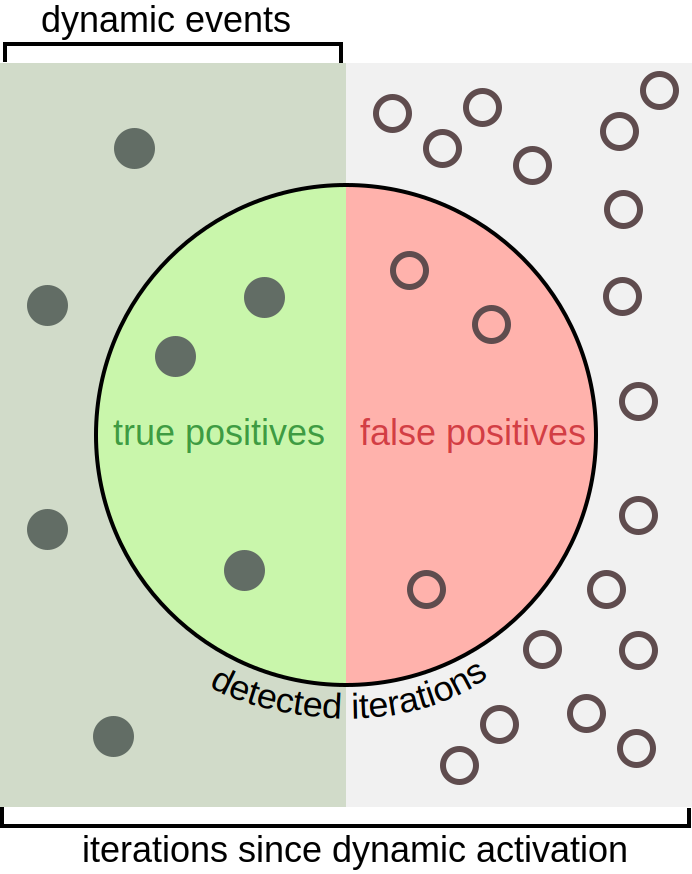
\includegraphics[width=0.45\textwidth]{dynamic_detection.svg}
	\caption[Illustration of iteration classification for dynamic problems]{Illustration of iteration classification for dynamic problems. Each dot represents one iteration between 2000 and 2600. The circle depicts all iterations where \gls{hsppbo} detected a dynamic change and therefore triggered the change handling procedure.}
	\label{fig:dynamic_detection}
\end{figure}

% !TeX root = main.tex
% !TeX spellcheck = en-US
% !TeX encoding = utf8


\chapter{Results and Evaluation}
\label{chap:results}

All experiments and analyses were performed as previously described in \cref{chap:testing,chap:analysis}. 

\section{Part I - Choosing the Optimization Algorithm}
\label{chap:part1}
The results of the first experimentation part are very insightful and allow for a sound analysis of the most appropriate optimization algorithm to tune the parameters of the \gls{hsppbo} algorithm. Note that an evaluation of the quality of the solution itself and of the performance of the \gls{hsppbo} algorithm is not discussed in this first part. The solution quality is only used to compare the optimization methods. 

\begin{figure}[h]
	\centering
	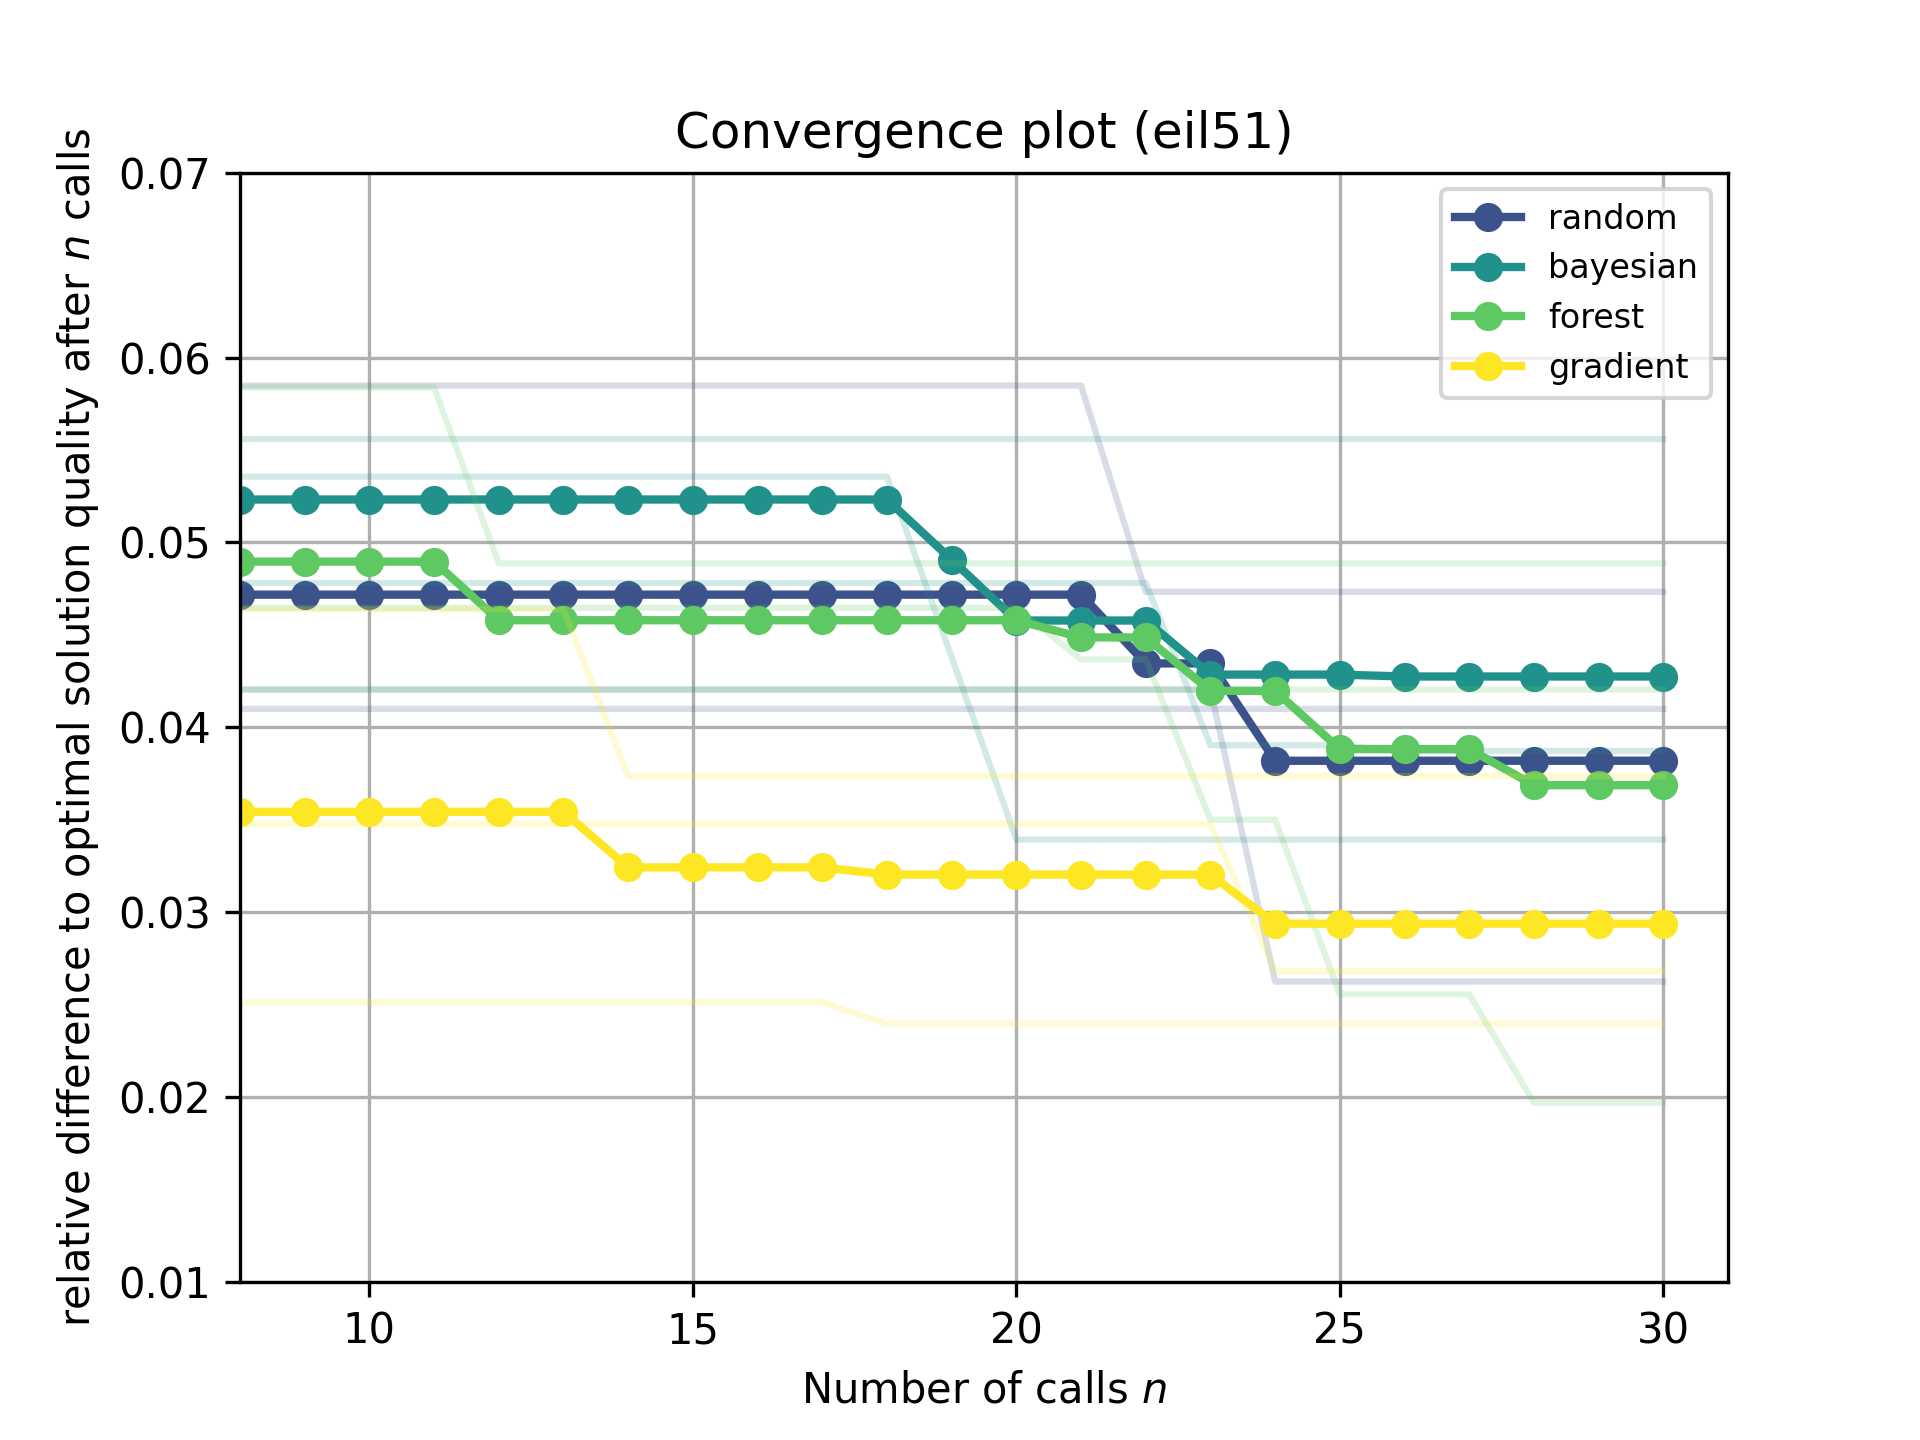
\includegraphics[width=0.75\textwidth]{results/part1/convergence_eil51.png}
	\caption[Convergence plot of \gls{tsp} instance \texttt{eil51}]{Convergence plot of \gls{tsp} instance \texttt{eil51}, comparing four different optimization algorithms.}
	\label{fig:convergence_eil51}
\end{figure}

First, the convergence plots of all five individual instances and their average are discussed. As explained in \cref{chap:an-part1}, these graphs show the minimum of the relative difference to the optimal solution $RPD$ up to each objective function call (\texttt{n\_call}). \cref{fig:convergence_eil51} shows this plot for the \texttt{eil51} \gls{tsp} instance. The bold, yellow line, which shows the average of the three \gls{gbrt} runs, indicates that this algorithm found the best solution over the course of the 30 objective calls. Except for a single run, where \gls{et} performed admirably, achieving a 2\% difference from the optimal solution, none of the other algorithms were able to come close to \gls{gbrt}. However, the average convergence behavior of all four algorithms seems to be very similar, with moderate improvements between objective calls 17 and 25. This behavior suggests that the first 10 sampling calls were sufficient to obtain a decent parameter configuration for the \texttt{eil51} instance. The specific runs (light colored lines) show that \gls{rs} and \gls{et} fluctuated the most in terms of initial solution quality and improvement over time. Although \gls{gp} produced the worst solutions out of all four algorithms, it still managed to achieve an average solution quality of almost 4\% after the full 30 \texttt{n\_calls}.

\begin{figure}[h]
	\centering
	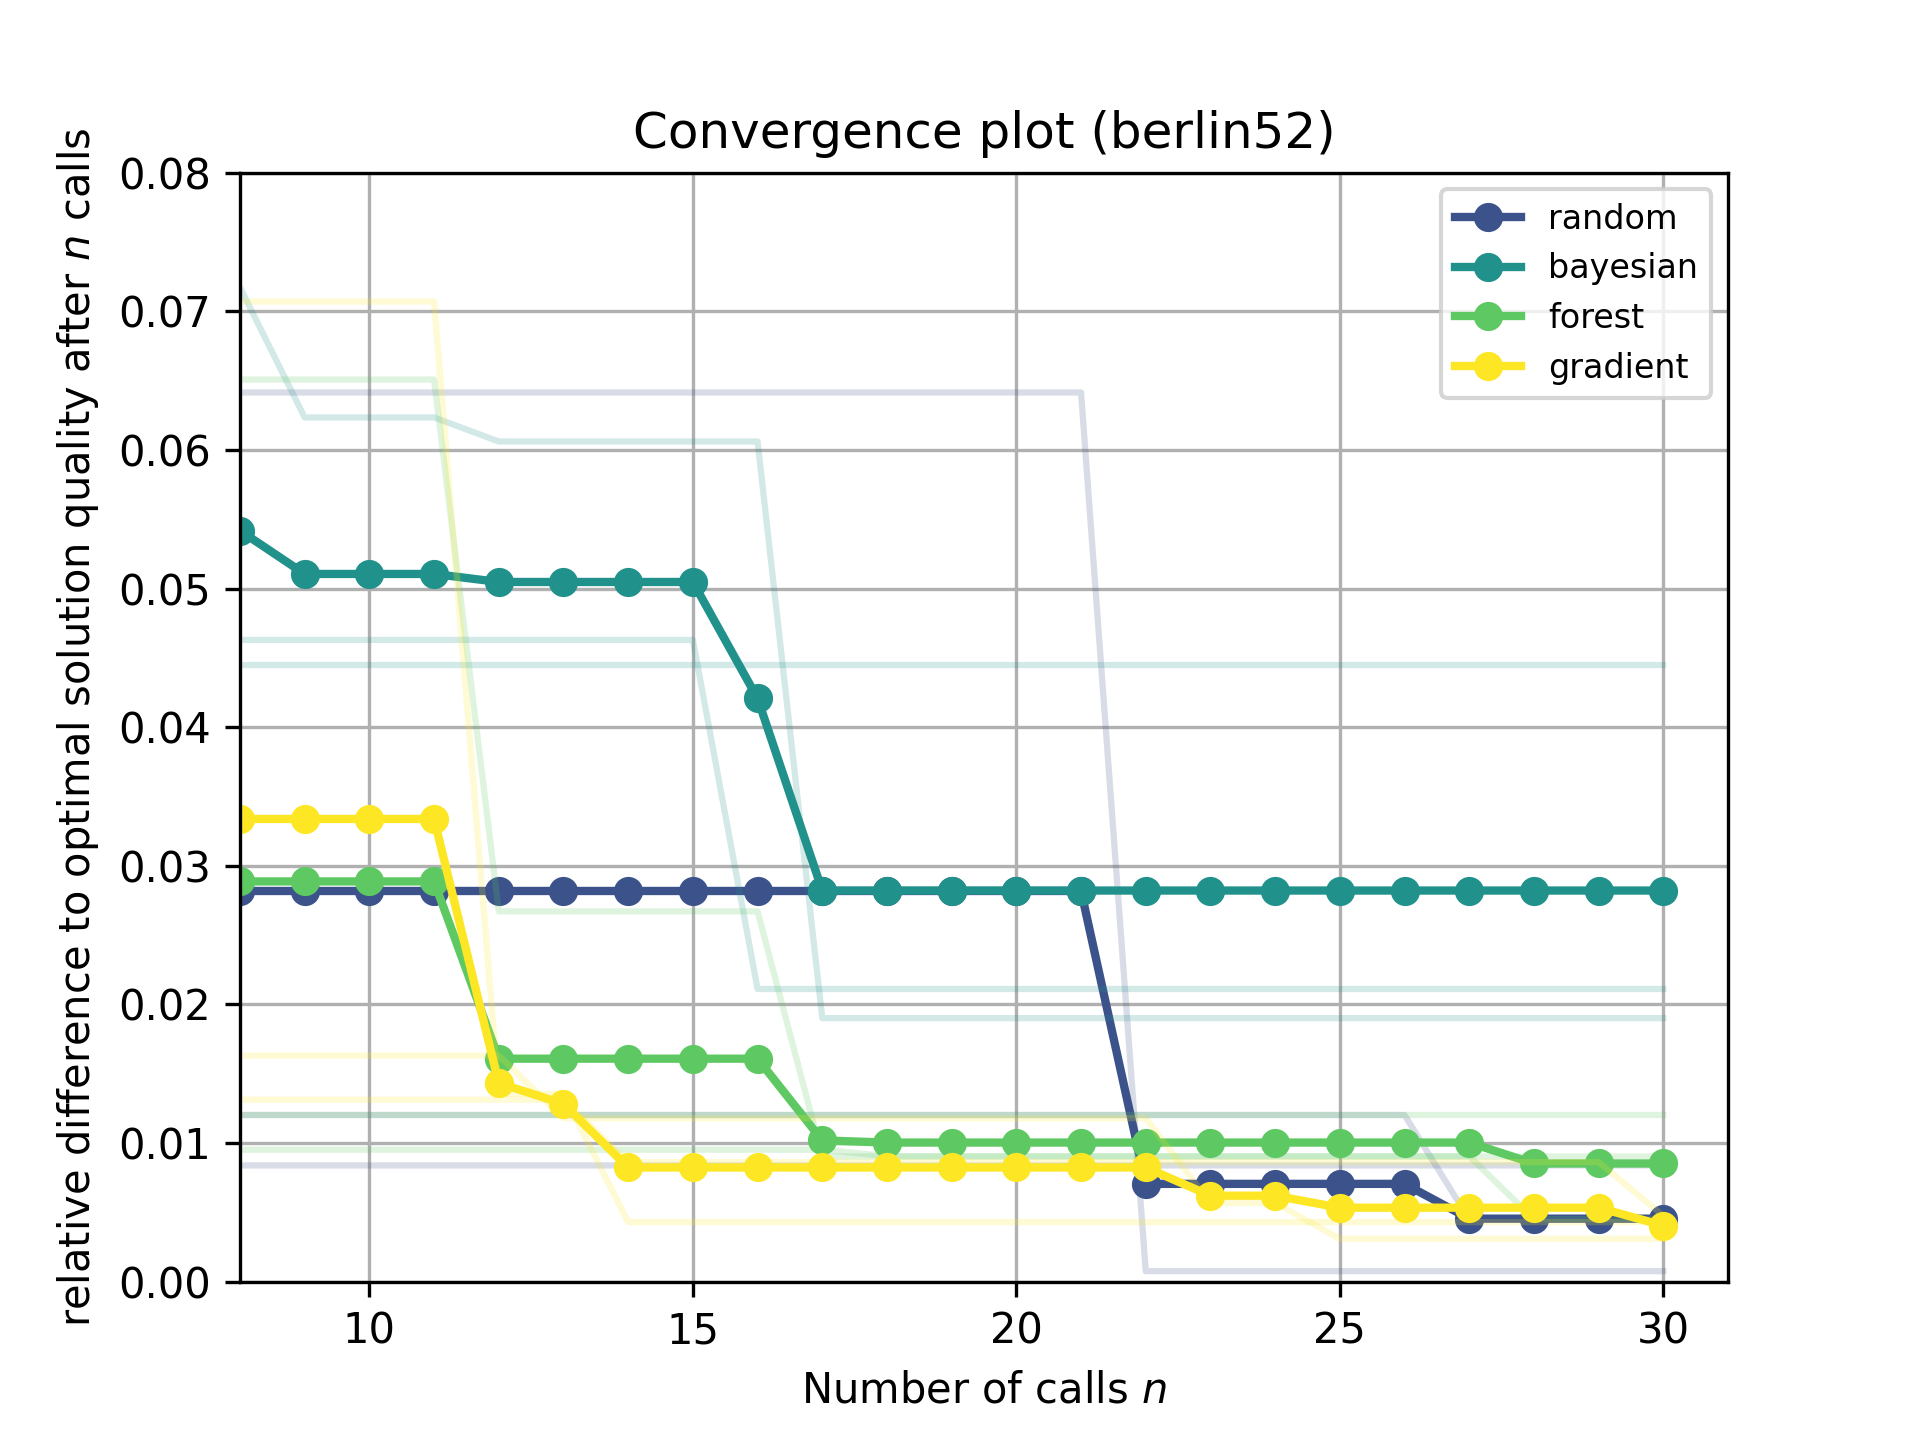
\includegraphics[width=0.75\textwidth]{results/part1/convergence_berlin52.png}
	\caption[Convergence plot of \gls{tsp} instance \texttt{berlin52}]{Convergence plot of \gls{tsp} instance \texttt{berlin52}, comparing four different optimization algorithms.}
	\label{fig:convergence_berlin52}
\end{figure}

The next instance is \texttt{berlin52}, whose convergence plot is shown in \cref{fig:convergence_berlin52}. Here, \gls{gp} continues to be the least well performing \gls{hpo} method, with a final average $RPD$ of only about 3\%, with one particular run reaching as low as $4.5\%$. All other methods achieved at least 2\% lower $RPD$ values, with \gls{rs} and \gls{gbrt} having an almost identical final $RPD$ of 0.5\%. 
However, \gls{gp} was able to improve its solution by a significant 2\% over the course of seven additional objective calls, suggesting that the algorithm was quickly making use of the now utilized, underlying model.
Due to the very random nature of \gls{rs}, some other individual runs started with a very high $RPD = 6.5\%$ and then, improved very abruptly after about 21 objective calls. The convergence behavior of \gls{rf} and \gls{gbrt} is quite similar and shows that both started with a good solution already at about 3\% for the tenth objective call, and then gradually improved up to objective call 17, analogous to \gls{gp}, but with less relative improvement. After that, only small gains in solution quality were achieved.

\begin{figure}[h]
	\centering
	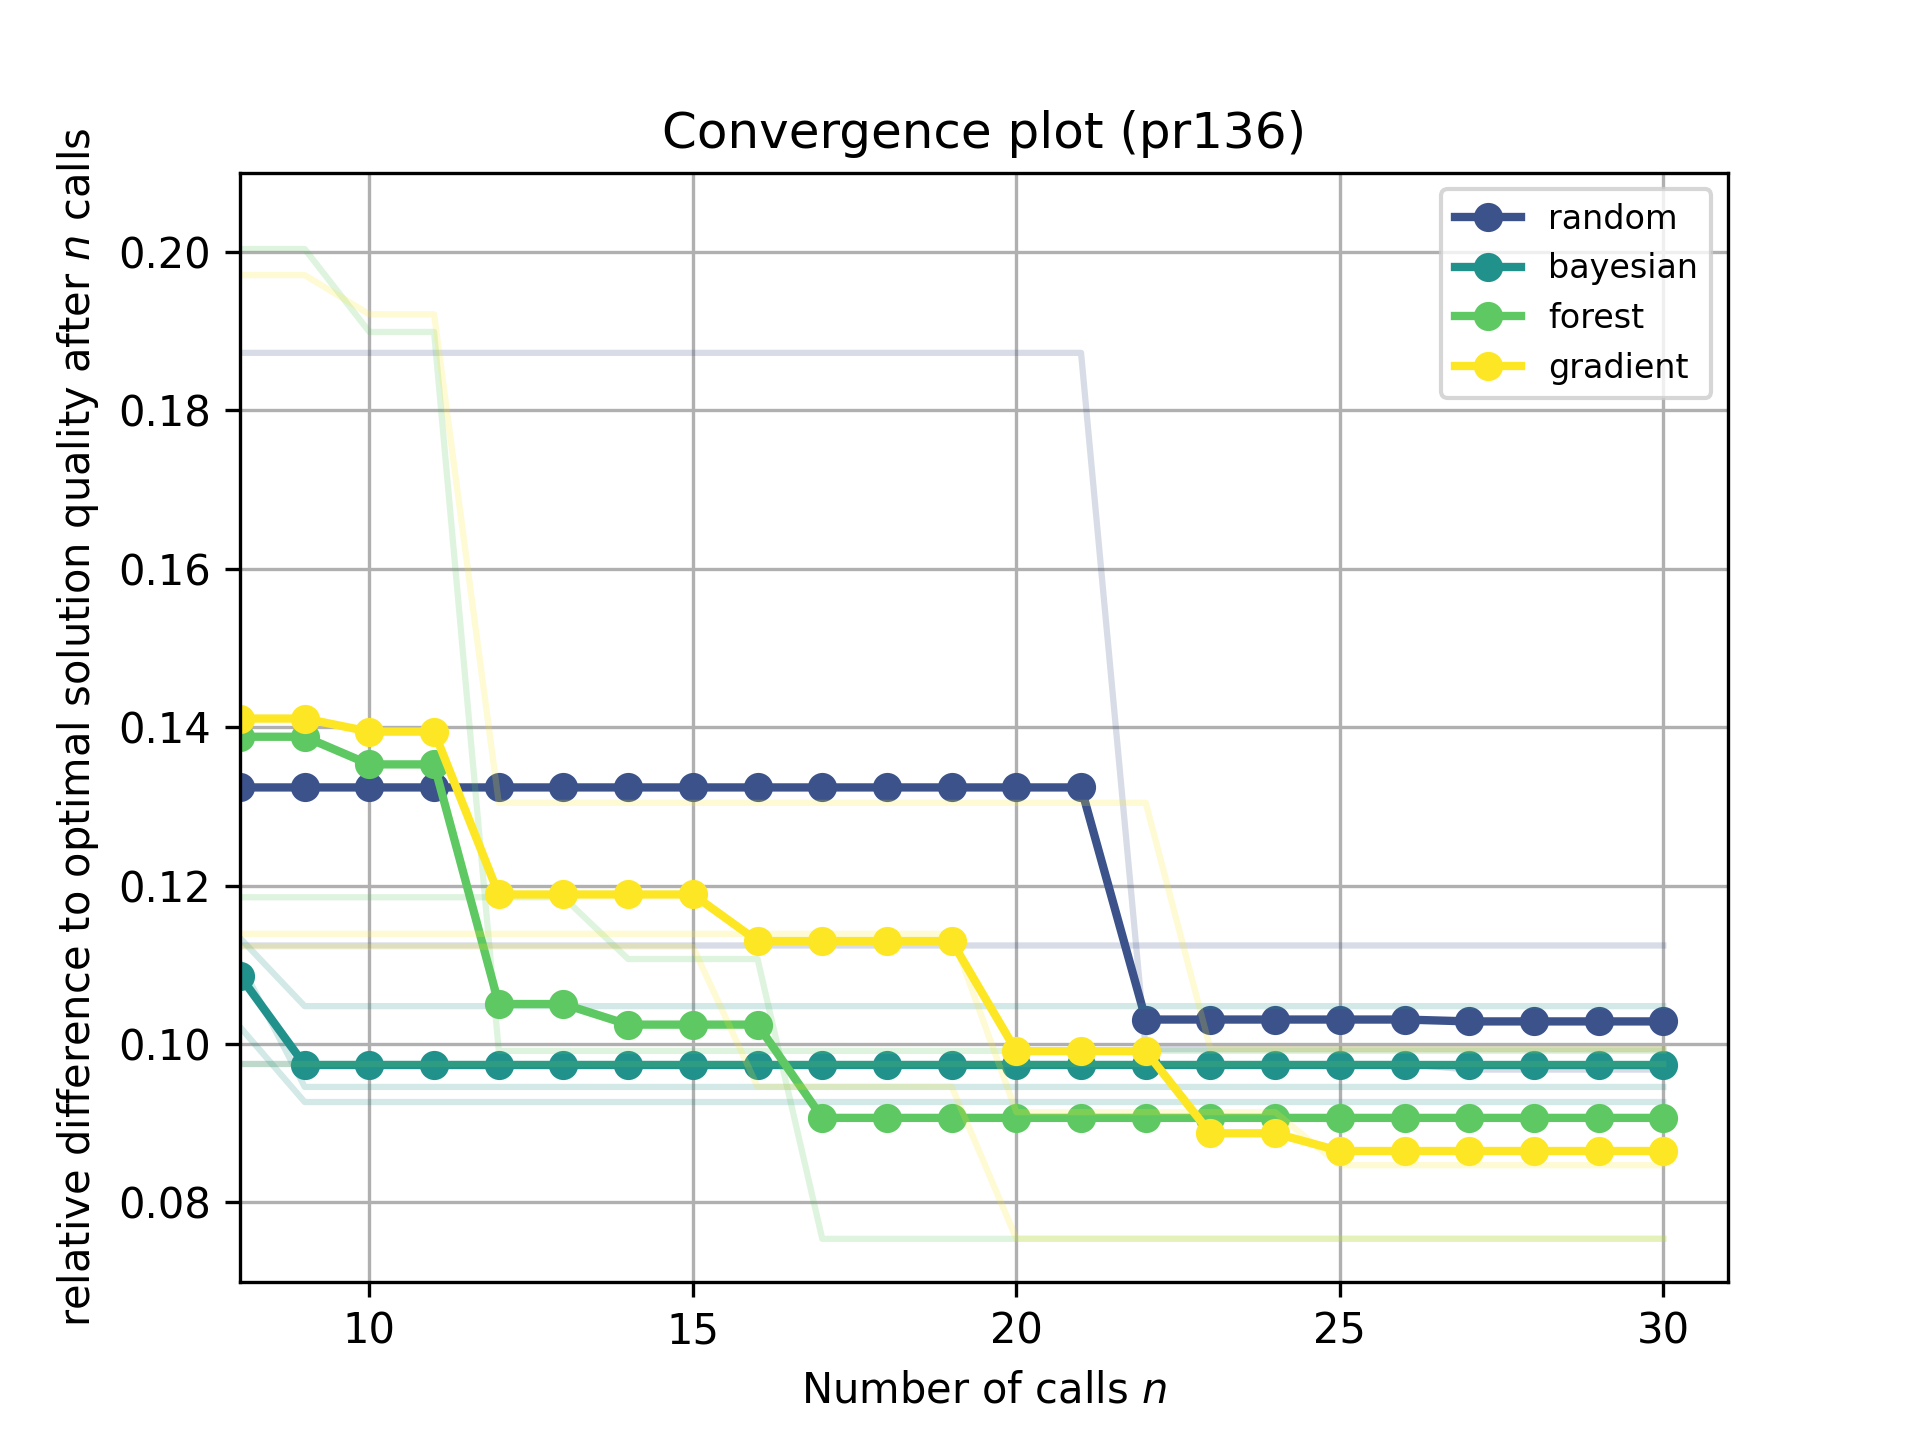
\includegraphics[width=0.75\textwidth]{results/part1/convergence_pr136.png}
	\caption[Convergence plot of \gls{tsp} instance \texttt{pr136}]{Convergence plot of \gls{tsp} instance \texttt{pr136}, comparing four different optimization algorithms.}
	\label{fig:convergence_pr136}
\end{figure}

The \texttt{pr136} \gls{tsp} instance, presented in \cref{fig:convergence_pr136}, continues the trend of \gls{gbrt} performing the best of the four optimization algorithms, albeit with a small lead of less than 0.5\% over the next best method, \gls{et}. Interestingly, \gls{gp} started with a considerably better initial sample at $RPD = 11\%$ after 10 objective calls, which gave it a head start, but also caused the algorithm to stagnate over the course of the remaining 20 calls. This might be due to the fact that Hammersley sampling was chosen only for this particular algorithm, or it could just be another random influence. \gls{et} and \gls{gbrt} gradually improved the most out of the four methods, with steep drops of around 2\% or more by the 23rd objective call. \gls{rs} rarely saw any meaningful improvement after the initial sampling, and the huge drop in average $RPD$ was due only to a single run that remained at a relatively poor value of $RPD = 18.8\%$ up until the 21st \texttt{n\_call}.

\begin{figure}[h]
	\centering
	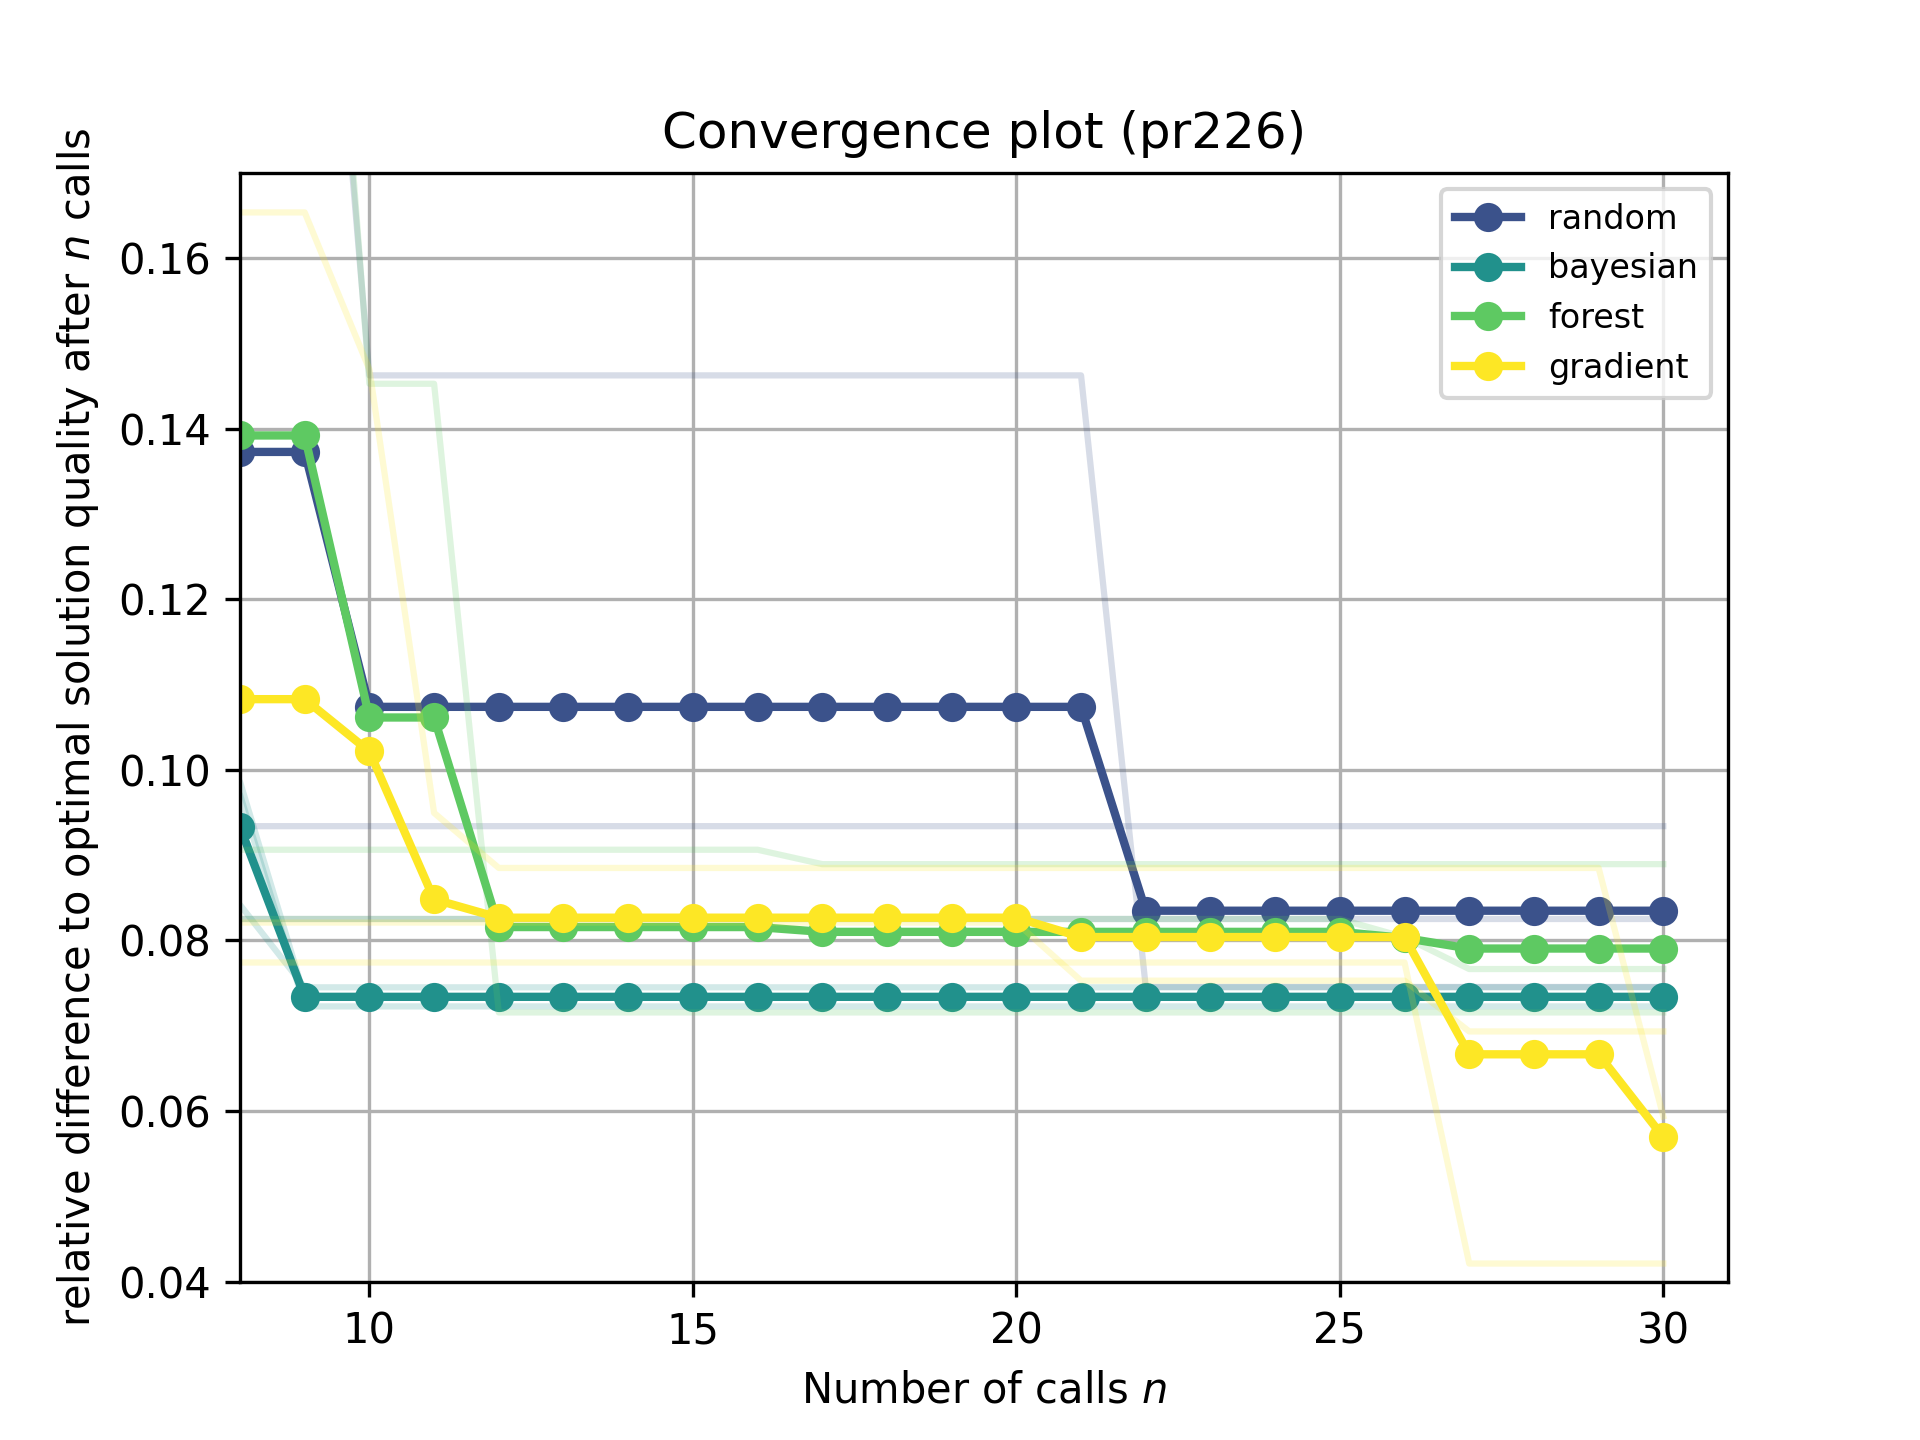
\includegraphics[width=0.75\textwidth]{results/part1/convergence_pr226.png}
	\caption[Convergence plot of \gls{tsp} instance \texttt{pr226}]{Convergence plot of \gls{tsp} instance \texttt{pr226}, comparing four different optimization algorithms.}
	\label{fig:convergence_pr226}
\end{figure}

The convergence plot in \cref{fig:convergence_pr226} for instance \texttt{pr226} again has \gls{rs} as the weakest method, with only small gains of about 2\% on objective call 22, bringing it to the average $RPD$ of the other algorithms. Some other single runs performed even worse. Contrary to the good performance of the other instances, this time \gls{et} starts its model training at 10 objective calls with a $RPD$ value almost the same as \gls{rs}, and only manages to significantly improve its parameters two \texttt{n\_calls} later. It then shows stagnant behavior at $RPD = 8\%$. Apart from the last five objective calls \gls{gbrt} showed a similar convergence behavior, improving by more than 2\% near the end, giving it the lead over \gls{gp}. This suggests that with larger instance dimensions and thus potentially more complex solutions, \gls{gbrt} benefits from more objective calls that improve the underlying model.
As with \texttt{pr136}, the initial sample of the Hammersley method potentially gave \gls{gp} a lead in solution quality, but then stagnated after the ninth call and was unable to improve its $RPD$ value of about 7.5\%.

\begin{figure}[h]
	\centering
	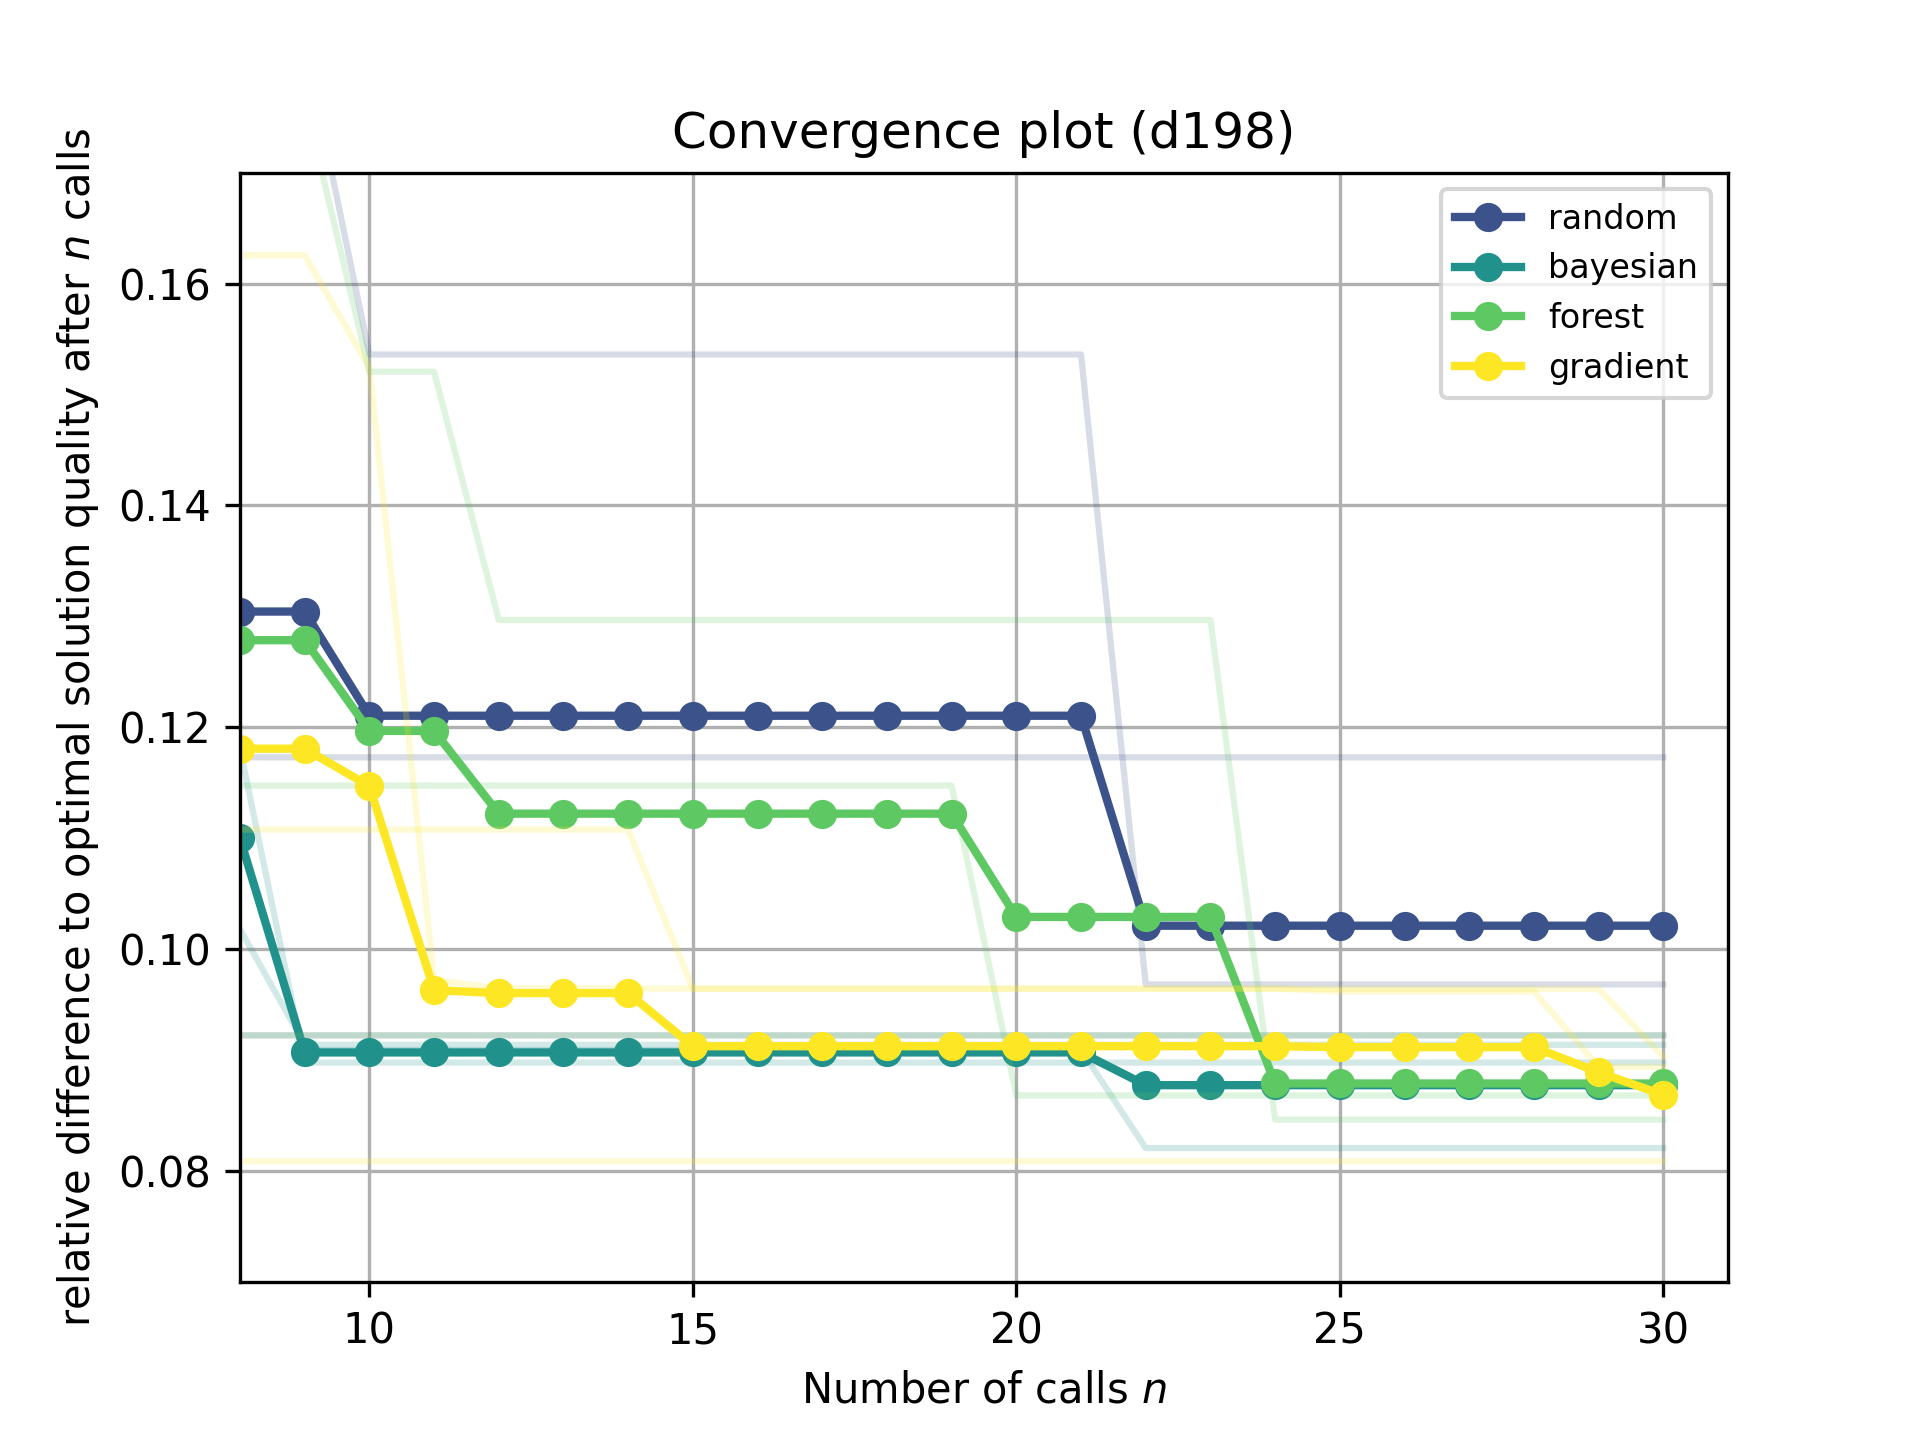
\includegraphics[width=0.75\textwidth]{results/part1/convergence_d198.png}
	\caption[Convergence plot of \gls{tsp} instance \texttt{d198}]{Convergence plot of \gls{tsp} instance \texttt{d198}, comparing four different optimization algorithms.}
	\label{fig:convergence_d198}
\end{figure}

The last \gls{tsp} instance, \texttt{d198}, confirms the observations of the previous instances, but this time all methods except \gls{rs} are within very close proximity of each other after the 24th objective call. Although \gls{gbrt} takes the lead in final relative solution quality with just under 9\%, it is not by much. Together with \gls{gp}, both methods managed to achieve considerable improvements up until the 15th objective call, after which they more or less stagnated. \gls{et} started with a similarly sub-optimal $RPD$ as \gls{rs} at objective call 10, but was able to improve steadily over the next 15 \texttt{n\_calls}. As expected at this point, \gls{rs} only managed to meaningfully improve in one run at objective call 21, still placing its final $RPD$ more than 1\% above the rest of the methods.

\begin{figure}[h]
	\centering
	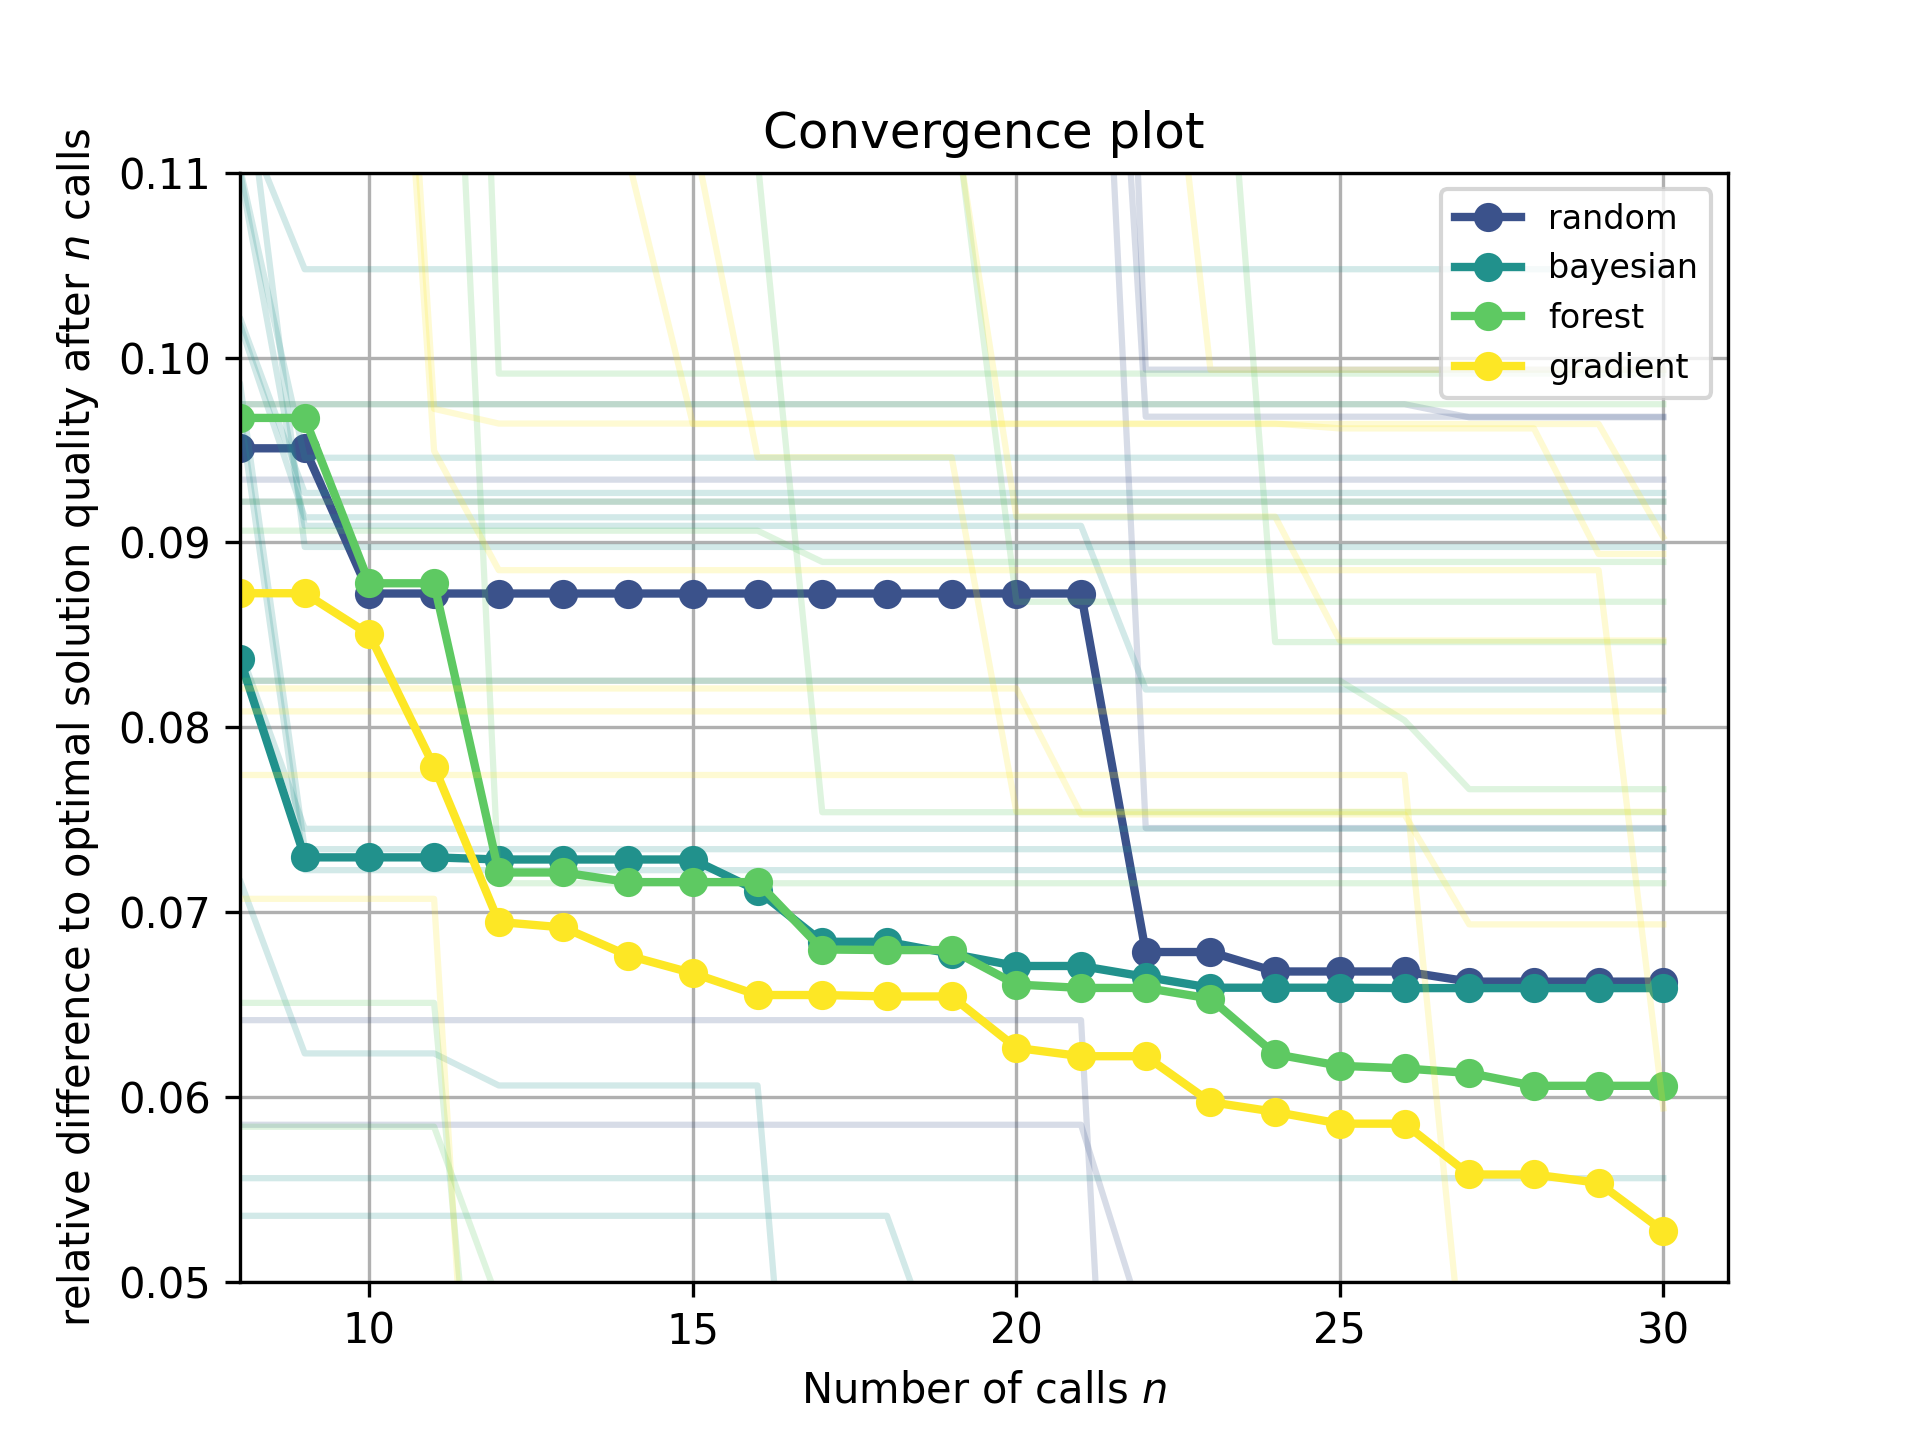
\includegraphics[width=0.75\textwidth]{results/part1/convergence_all.png}
	\caption[Convergence plot of the average over five \gls{tsp} instances]{Convergence plot of the average over five \gls{tsp} instances \texttt{eil51, berlin52, pr136, pr226, d198}, comparing four different optimization algorithms.}
	\label{fig:convergence_all}
\end{figure}

Lastly, the average convergence plot aggregates the runs of all five instances. Since \gls{gbrt} is the best performing method out of all the individual comparisons, its average convergence behavior emphasizes this by giving it a lead in final $RPD$ of about 1.5\% over the next best method, \gls{et}. Both methods show similar convergence behavior over the entire runtime, with large improvements in the first few objective calls, and small, but steady (almost linear) improvements thereafter. The behavior of \gls{gp} is not very different from previous descriptions, and is mainly distinguished by its better initial $RPD$ value, which reinforces the proposed relationship with the Hammersley sampling method. After this initial lead, the algorithm almost stagnates, and after the 22nd objective call, it converges to the trajectory of \gls{rs}.

\begin{table}[h]
	\centering
	\caption[The \gls{auc} and $RPD_{min}$ for all optimization runs]{The \gls{auc} and minimum relative solution quality at the last objective call ($RPD_{min}$) of all optimization runs for each method and instance, and for the mean over all instances.}
	\label{tab:part1-stats}
	\begin{tabular}{l c c c  c  c  c }
		 \hline
		~ & \multicolumn{2}{c}{eil51} &  \multicolumn{2}{c}{berlin52} &  \multicolumn{2}{c}{pr136} \\
		\cmidrule(lr){2-3} \cmidrule(lr){4-5} \cmidrule(lr){6-7}
		~ & \gls{auc} & $RPD_{min}$ & \gls{auc} & $RPD_{min}$ & \gls{auc} & $RPD_{min}$ \\ \noalign{\hrule height 1pt}
		RS & 0.830 & 0.026 & 0.347 & 0.001  & 2.266 & 0.097 \\
		GP & 0.900 & 0.034 & 0.650 & 0.019 & 1.850 & 0.093 \\ 
		ET & 0.819 & 0.020 & 0.227 & 0.005 & 1.809 & 0.075 \\ 
		GBRT & 0.601 & 0.024 & 0.159 & 0.003 & 1.948 & 0.075 \\ \noalign{\hrule height 1pt}
	\end{tabular}
	\bigskip\\
	\begin{tabular}{l  c  c  c  c  c  c}
	   \hline
		~ & \multicolumn{2}{c}{pr226} & \multicolumn{2}{c}{d198} & \multicolumn{2}{c}{mean}\\
		\cmidrule(lr){2-3} \cmidrule(lr){4-5} \cmidrule(lr){6-7}
		~ & \gls{auc} & $RPD_{min}$ & \gls{auc} & $RPD_{min}$ & \gls{auc} & $RPD_{min}$ \\ \noalign{\hrule height 1pt}
		RS &  1.837 & 0.075 & 2.139 & 0.092 & 1.484 & 0.058\\ 
		GP & 1.394 & 0.072 & 1.698 & 0.082 & 1.298 & 0.060\\
		ET & 1.547 & 0.072 & 1.940 & 0.085 & 1.268 & 0.051\\ 
		GBRT & 1.497 & 0.042 & 1.745 & 0.081 & 1.190 & 0.045\\ \noalign{\hrule height 1pt}
	\end{tabular}
\end{table}

Regarding the visually observable convergence behavior of the four optimization methods, we can also look at the \glsfirst{auc} of the plots and the minimum/best relative solution quality obtained, i.e. the $RPD$ value at $\texttt{n\_call} = 30$, hereafter called $RPD_{min}$. This data is presented in \cref{tab:part1-stats}, averaged over all available optimizer runs, for all five instances, and their mean.
In this context, a low \gls{auc} value indicates that the optimization algorithm found a well-performing parameter set, and therefore a low $RPD$, in a short time, i.e., few objective calls. However, the comparatively lowest \gls{auc} does not necessarily mean that it also found the lowest $RPD_{min}$ value among all algorithms. Thus, both values are discussed for each instance to determine how fast each algorithm converged to its best solution. For the \texttt{eil51} \gls{tsp} instance, \gls{gbrt} has by far the lowest \gls{auc} of 0.601. Paired with the second best $RPD_{min} = 2.4\%$, this method continues its favorable performance from the convergence plots. With a 0.4\% improvement in $RPD_{min}$ over \gls{gbrt}, \gls{et} was the second fastest to convergence to this final solution. \gls{gp} delivered the worst performance in this instance.

The \texttt{berlin52} instance implies a similar behavior, with \gls{gbrt} leading in convergence speed with the lowest \gls{auc}. However, as discussed in the corresponding convergence plot, \gls{rs} managed to find the best solution out of the four methods, with $RPD_{min} = 0.1\%$, outperforming \gls{gbrt} by 0.2\%. Again, \gls{gp} shows the worst performance, this time with an \gls{auc} of $0.650$, almost twice as high as its direct competitor \gls{rs} with $0.347$. \gls{et} is again the second fastest converging algorithm after \gls{gbrt}, with an almost equally good $RPD_{min} = 0.5\%$.

The results for \texttt{pr136} show an equal best $RPD_{min} = 7.5\%$ for \gls{gbrt} and \gls{et}, and an almost equal \gls{auc} for \gls{gp} and \gls{et}. Therefore, in this instance, \gls{et} outperforms \gls{gbrt} as the best converging algorithm. Interestingly, even \gls{gp} achieves a better \gls{auc} of $1.850$ than \gls{gbrt}, albeit with a worse minimum relative solution quality, which is more in line with \gls{rs}.

\texttt{pr226}, the largest \gls{tsp} instance out of the five tested in this part of the experimentation discussion, continues the improvement of \gls{gp} in terms of \gls{auc}, resulting in the best value out of all four algorithms, with a solid 7\% difference compared to the next best algorithm, \gls{gbrt}, which itself, was able to achieve the best $RPD_{min}$ at 4.2\%. \gls{rs} continues to perform worse as the instance dimension increases, which could be an opposite trend for the convergence speed of \gls{gp}.

The last \gls{tsp} instance, \texttt{d198}, confirms this implication, resulting in \gls{gp} again being the best algorithm in terms of \gls{auc}, and the second best in terms of $RPD_{min}$ at 8.2\%. This suggests, that this algorithm could benefit from larger, more complex instances, perhaps even from stronger clustering, as the latter two instances were categorized. \gls{gbrt} achieved the best $RPD_{min}$ value at 8.1\% and the second best \gls{auc}, which is only 2.7\% higher than the value of \gls{gp}. In this instance, the performance of \gls{et} was comparatively underwhelming, being closer to the \gls{auc} value of \gls{rs} than to the other two methods.

Finally, the mean results confirms that \gls{gbrt} was the algorithm that converged the fastest ($\gls{auc} = 1.19$) to the best performing parameter set ($RPD_{min} = 4.5\%$). Even in later, higher dimensional  instances, it performed at least the second best or better, implying good search consistency across the parameter space. \gls{et} obtained better solutions for the three smaller instances, resulting in lower averages compared to \gls{gp}, which showed the opposite trend, improving with higher problem dimension.

\begin{figure}[h]
	\centering
	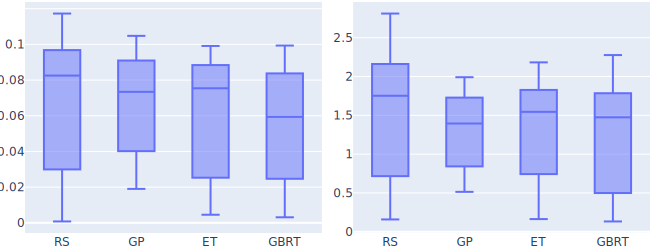
\includegraphics[width=\textwidth]{results/part1/convergence_stats_boxplot.svg}
\captionsetup[subfigure]
{skip=-8pt}
		\hfill
		\subcaptionbox{Relative difference to optimal solution quality at last the objective call ($RPD_{min}$) for all runs and instances.\label{fig:convergence_stats_boxplot_rpd_min}}[.45\linewidth]{\hfill}
		\hfill
		\subcaptionbox{\Glsfirst{auc} of solution quality convergence graph.\label{fig:convergence_stats_boxplot_auc}}[.45\linewidth]{\hfill}

	\caption[Statistical box plots illustrating convergence plots]{Statistical box plots illustrating the data of all five individual convergence plots and their individual runs.}
\label{fig:convergence_stats_boxplots}
\end{figure}

\Cref{fig:convergence_stats_boxplots} shows statistical box plots for both of the metrics from the table over all runs and data from all problem instances combined. This visualization is also used to evaluate the consistency across all four optimization methods, which was previously only implied by their average or best-case performance. However, this is not normalized by instance, so the absolute values and differences, as with the mean from the previous table, might not be as expressive. Nevertheless, since all four algorithms are affected by this bias, qualitative statements are still possible.

The dispersion of $RPD_{min}$ in \cref{fig:convergence_stats_boxplot_rpd_min} implies that \gls{gp} reached its solution most consistently at around its median of 7.5\%, but also never reached the same minimum as the other three algorithms. \gls{rs}, on the other hand, was the most unreliable method, with its maximum and minimum being far of from the upper and lower quartiles, respectively. It also has the highest median at about 8\%. \gls{gbrt} and \gls{et} share similarities in their \gls{iqr} and minimum/maximum values, with \gls{gbrt} having a slightly smaller dispersion. However, they differ tremendously in their median, with \gls{et} having a value almost 2\% higher than \gls{gbrt}, which means that although both their solution consistency is not ideal, \gls{gbrt} still obtained the best final solution out of all algorithms.

The box plots for the \gls{auc} (\cref{fig:convergence_stats_boxplot_auc}) show similar consistency behavior. \gls{gp} is again the most reliable algorithm when it comes to converging to its final solution, but again it cannot provide the same best-case performance (minimums) as the other three algorithms. Howeer, its median is the lowest, with \gls{gbrt} having the second lowest value, but also a significantly higher \gls{iqr} than \gls{gp}. Lastly, \gls{rs} shows the most inconsistent behavior with the highest median. 

\subsection{Statistical Tests}

To validate all of the above results, two statistical tests were also performed on the optimization data. The first test was the Kruskal–Wallis H test, explained in section \cref{chap:kruskal}, with each of the four optimization algorithms as a sample group, and separated by the five instances used. The results for each instance are shown in \cref{tab:kruskal-test}. A common significance level of 0.05 was chosen to reject the null hypothesis. The data from the table shows that for each of the five instances, we can definitely reject the null hypothesis by looking at the $p$-values, thus suggesting that the four optimization algorithms show a significantly different convergence behavior from each other. 

\begin{table}[h]
	\centering
	\caption[Results of the Kruskal–Wallis H test for all optimization run data of the first part]{Results of the Kruskal–Wallis H test for all optimization run data of the first part, with each of the four optimization algorithms as a sample group, separated by \gls{tsp} instance.}
	\label{tab:kruskal-test}
	\begin{tabular}{l | l  l  l  l  l }
		 \hline
		~ & eil51 & berlin52 & pr136 & pr226 & d198 \\ \hline
		statistic & 47.893 &	46.960&	29.898	&57.998	&46.514 \\
		$p$-value & \num{2.244e-10} & \num{3.544e-10} &\num{1.450e-6} & \num{1.574e-12} & \num{4.410e-10} \\ \hline
	\end{tabular}
\end{table}
\texttt{}

A post-hoc Conover–Iman test was then performed to gain more insight into which specific pairs of optimization algorithms differ and how. As explained in \cref{chap:conover}, a one-sided test was used, resulting in two tables - one for the statistic value (\cref{tab:conover-t}) and one for the $p$-value (\cref{tab:conover-p}). Note that this table format was preferred over a symmetric matrix for each problem instance, with the columns and rows containing all five methods each. As presented here, redundant information can be excluded by directly pairing the algorithms, resulting in $\binom{4}{2} = 6$ pairs (columns) for each \gls{tsp} instance (rows). 

Starting with the $p$-value to reject the null hypothesis, we can then look at the statistic value, more specifically at the sign, to formulate the alternative hypothesis, i.e. to infer how the distribution of the convergence behavior for the algorithms differ. A positive value implies that in this particular pairwise comparison (X vs. Y), the first stated algorithm (X) has a distribution that is significantly above the others, suggesting that either the convergence speed, the solutions obtained, or both, are also worse than the second one (Y). Furthermore, in both tables the cells are marked green, whenever the $p$-value is lower than 0.05 (the significance level) and the null hypothesis can be rejected for that combination of \gls{tsp} instance and optimization method pairing.

\begin{table}[h]
	\centering
	\caption[The $p$-value of the Conover–Iman test for all optimization run data of the first part]{The $p$-value of the Conover–Iman test for all optimization run data of the first part, with each of the four optimization algorithms as a sample group, separated by \gls{tsp} instance. The cells are marked green, whenever the $p$-value is lower than the significance level of $0.05$.}
	\label{tab:conover-p}
	
	\begin{adjustbox}{width=1\textwidth}
		\begin{tabular}{ l | l  l  l  l  l  l}
			\hline
			TSP & \gls{rs} vs. \gls{gp} & \gls{rs} vs. \gls{et} & \gls{rs} vs. \gls{gbrt} & \gls{gp} vs. \gls{et} & \gls{gp} vs. \gls{gbrt} & \gls{et} vs. \gls{gbrt} \\ \hline
			eil51 & \num{0.626022837} & \num{1} & \cellcolor{green!25} \num{1,3613E-11} & \cellcolor{green!25} \num{0,045498418} &  \cellcolor{green!25} \num{9,87937E-15} &\cellcolor{green!25}  \num{1,71033E-09} \\ 
			berlin52 & \cellcolor{green!25} \num{6,31757E-10} & \num{1} & \num{0,055983678} & \cellcolor{green!25} \num{4,84375E-08} & \cellcolor{green!25} \num{5,09448E-15} & \cellcolor{green!25} \num{0,002694824} \\
			pr136 & \cellcolor{green!25} \num{4,40687E-06} &\cellcolor{green!25}  \num{1,47269E-07} & \cellcolor{green!25} \num{1,49122E-04} & \num{1} & \num{1} & \num{0,524644367} \\
			pr226 & \cellcolor{green!25} \num{1,07734E-22} & \cellcolor{green!25} \num{1,85077E-10} & \cellcolor{green!25} \num{1,83947E-11} & \cellcolor{green!25} \num{2,22893E-08} & \cellcolor{green!25} \num{2,06853E-07} & \num{1} \\ 
			d198 & \cellcolor{green!25} \num{4,0384E-15} & \cellcolor{green!25} \num{0,001090407} & \cellcolor{green!25} \num{2,6556E-07} & \cellcolor{green!25} \num{1,20061E-07} & \cellcolor{green!25}  \num{0,000563675} & \num{0,210301266}  \\ \hline
		\end{tabular}
	\end{adjustbox}
\end{table}

\begin{table}[h]
	\centering
	\caption[The $p$-value of the Conover–Iman test for all optimization run data of the first part]{The statistical value of the Conover–Iman test for all optimization run data of the first part, with each of the four optimization algorithms as a sample group, separated by \gls{tsp} instance. The cells are marked green, whenever the $p$-value is lower than the significance level of $0.05$.}
	\label{tab:conover-t}
	
	\begin{adjustbox}{width=1\textwidth}
	\begin{tabular}{ l | l  l  l  l  l  l}
		\hline
		TSP & \gls{rs} vs. \gls{gp} & \gls{rs} vs. \gls{et} & \gls{rs} vs. \gls{gbrt} & \gls{gp} vs. \gls{et} & \gls{gp} vs. \gls{gbrt} & \gls{et} vs. \gls{gbrt} \\ \hline
		eil51 & \num{-1,643854208} & \num{1,099460932} & \cellcolor{green!25} \num{8,358037955} & \cellcolor{green!25} \num{2,74331514} & \cellcolor{green!25} \num{10,00189216} & \cellcolor{green!25} \num{7,258577024} \\
		berlin52 & \cellcolor{green!25} \num{-7,486334021} & \num{-1,00169258} & \num{2,667665503} & \cellcolor{green!25} \num{6,484641441} & \cellcolor{green!25} \num{10,15399952} & \cellcolor{green!25} \num{3,669358084} \\ 
		pr136 & \cellcolor{green!25} \num{5,39986544} & \cellcolor{green!25} \num{6,222702079} & \cellcolor{green!25} \num{4,491316652} & \num{0,822836638} & \num{-0,908548788} & \num{-1,731385427} \\ 
    	pr226 & \cellcolor{green!25} \num{14,43190942} & \cellcolor{green!25} \num{7,765991183} & \cellcolor{green!25} \num{8,289835445} & \cellcolor{green!25} \num{-6,665918233} & \cellcolor{green!25} \num{-6,142073971} & \num{0,523844262} \\ 
    	d198 & \cellcolor{green!25} \num{10,20744357} & \cellcolor{green!25} \num{3,936409009} & \cellcolor{green!25} \num{6,082589453} & \cellcolor{green!25} \num{-6,271034565} & \cellcolor{green!25} \num{-4,124854122} & \num{2,146180444} \\ \hline
	\end{tabular}
	\end{adjustbox}
\end{table}

The data from both tables show that the distribution of the \gls{gbrt} method is below all other algorithms for the \texttt{eil51} instance, although the null hypothesis in the pairing with \gls{et} was only slightly below the significance level. Furthermore, the distribution of \gls{et} was also below that of \gls{gp}, confirming the visual inference from the convergence plot. 
In the data for the \texttt{berlin52} instance, \gls{gbrt} is below \gls{gp} and \gls{et}, but interestingly, fails to reject the null hypothesis when compared to \gls{rs}, confirming the unrepresentatively good performance of this algorithm for this instance. Also, the convergence distribution of \gls{gp} is above all other three algorithms by comparison, which is also shown in \cref{fig:convergence_berlin52}.
For the next three instances, \texttt{pr136, pr226,} and \texttt{d198}, the distribution for \gls{rs} lies above all other three algorithms, verifying the underwhelming performance described in previous discussion. For the two latter instances, we can also determine that the convergence behavior of \gls{gp} is above the distribution of both \gls{et} and \gls{gbrt}.

In summary, \gls{rs} could establish itself as having a favorable distribution only once, \gls{et} managed to have a lower convergence behavior five times, \gls{gp} could undercut in its direct pairing seven times, and \gls{gbrt} was the optimization algorithm that fell below its comparison distribution the most with 10 times. All of this confirms the favorable position of \gls{gbrt}, but also strengthens the case for \gls{gp} over \gls{et}.

\subsection{Conclusion}

As expected, \glsfirst{rs} proved to be the worst performing algorithm under these test conditions. Although each of the other three methods was able to reliably outperform its solutions, usually with fewer objective calls, it still produced satisfactory solutions that differed from the rest by only a few percent. Therefore, its aforementioned position as a \enquote{baseline} \gls{hpo} method is more than justified.

The \glsfirst{gbrt} algorithm shows the fastest convergence with the best solution quality, while providing the second most robust results. Therefore, it is used to perform the second part of the testing procedure. Another advantage, besides its good performance, is its ability to provide a trained machine learning model from which the parameter importance and other qualitative statements about its prediction can be derived.

However, the theoretical second choice is not so clear, since both \glsfirst{gp} and \glsfirst{et}, performed very well in certain instances. As suggested in some earlier discussions, \gls{et} seems to perform its best on \gls{tsp} instances with less than 100 city nodes, while \gls{gp} improves its convergence and solutions significantly on \gls{tsp} instances with dimensions above 150. Another factor may be the city placement characteristic established in \cref{chap:problem-choice}. However, confirming this possible relationship would require a different experimental setup, whereas the data from this first part would not be sufficient. Therefore, both of these algorithms should be considered as potential candidates for future tests, especially with varying problem dimensions and complexity.


\section{Part II - Choosing the Parameter Sets}
\label{chap:part2}

The second part of the experiments was performed using only the \glsfirst{gbrt} optimization method, but this time with twice the objective calls and for all dynamic intensities applied to the smaller instances. Unlike the previous part, there was no need to manually select a \enquote{winner} based on the results, since the \gls{hpo} procedure provided six parameter sets and a corresponding solution quality ($RPD$) for each of the 15 combinations of problem instance and dynamic intensity $C$ (see \cref{tab:exp-setup}). From these, the best performing set with the lowest tour length $L$ was selected and is shown in \cref{tab:best-parameters}. The parameters were explicitly chosen by this quantifiable procedure to free the further analysis from any assumptions about the the parameter aggregation process other than solution quality. While it would have been possible to average each parameter set over its six optimizer runs, or even over different dynamic intensities or problem instances, this would have introduced many unknown influences and would have allowed speculation as to which averaging method would be the most beneficial.

\begin{table}[h]
	\centering
	\caption[Best parameters from all six optimizer runs for all 15 instance combinations]{Best parameters from all six optimizer runs for all 15 combinations of \gls{tsp} instance and dynamic intensity $C$ from the second part of the experiment.}
	\label{tab:best-parameters}
	\begin{tabular}{cc | ccccccc}
		\hline
		TSP & $C$ & $\alpha$ & $\beta$ & $w_{\text{persbest}}$ & $w_{\text{persprev}}$& $w_{\text{parentbest}}$ & $\theta$ & $H$ \\ \hline
		eil51 & 0.1 & 1 & 5 & \num{0.9698012032709232} & \num{0.4970104731148196} & \num{0.9420638486560448} & \num{0.3905213054442555} & partial \\ 
		eil51 & 0.25 & 2 & 9 & \num{0.1433513703862964} & \num{0.2385297997812011} & \num{0.5412435716306161} & \num{0.3635623273846985} & full \\ 
		eil51 & 0.5 & 2 & 10 & \num{0.0587705067002678} & \num{0.959991562647809} & \num{0.4867708232028435} & \num{0.4598096104688355} & full \\ 
		berlin52 & 0.1 & 3 & 9 & \num{0.0448916769013341} & \num{0.4777787643927934} & \num{0.1957091892595615} & \num{0.2759480271198957} & partial \\ 
		berlin52 & 0.25 & 2 & 8 & \num{0.8311455041131819} & \num{0.2222104051600784} & \num{0.313274428287894} & \num{0.436036995565174} & full \\ 
		berlin52 & 0.5 & 1 & 9 & \num{0.2485751505630211} & \num{0.7739840642032905} & \num{0.9723725969016688} & \num{0.3880068267237935} & partial \\ 
		pr136 & 0.1 & 2 & 8 & \num{0.0939741840300781} & \num{0.0084471729216077} & \num{0.4693720297474018} & \num{0.3863810991570361} & partial \\ 
		pr136 & 0.25 & 2 & 10 & \num{0.038003058216178} & \num{0.6873466028167179} & \num{0.9394324689971254} & \num{0.3901585164695582} & partial \\ 
		pr136 & 0.5 & 2 & 9 & \num{0.0728348279719507} & \num{0.3253009907927114} & \num{0.6673567555329409} & \num{0.1388609048589145} & partial \\ 
		pr226 & 0.1 & 2 & 10 & \num{0.1121258043746194} & \num{0.0511444733887272} & \num{0.4363901120147211} & \num{0.1826781698597669} & partial \\ 
		pr226 & 0.25 & 2 & 9 & \num{0.4883129003158867} & \num{0.4713032045025087} & \num{0.9389513559003996} & \num{0.2397757555252823} & partial \\ 
		pr226 & 0.5 & 2 & 9 & \num{0.4276386300373169} & \num{0.1532697969130651} & \num{0.9835424877972389} & \num{0.2913396086500334} & partial \\ 
		d198 & 0.1 & 2 & 9 & \num{0.0017540098159148} & \num{0.973965162760525} & \num{0.651535106135457} & \num{0.2115440416644889} & partial \\ 
		d198 & 0.25 & 2 & 10 & \num{0.6702515127832059} & \num{0.0903011306643848} & \num{0.891733065508089} & \num{0.3858381960233191} & full \\ 
		d198 & 0.5 & 2 & 10 & \num{0.6940812792792512} & \num{0.2167360884224609} & \num{0.6662157175599704} & \num{0.2163287362343122} & partial \\ \hline
	\end{tabular}
\end{table}

These best parameter results alone would have been sufficient to continue with the validation in the third part, as \gls{hpo} is intended to enhance and accelerate this parameter tuning process. However, there is much information to be gained from this data set in terms of robustness, correlation between parameters and with problem descriptions, and relative parameter importance. All of this provides insight into what most influences the \gls{hpo} process, and thus the performance of the \gls{hsppbo} metaheuristic.

\subsection{Robustness of Parameter Values}
\label{chap:robustness}

First, we look at how often a particular value for a given parameter was chosen by the \gls{hpo} and how reliable that choice is  - in short, the parameter robustness and dispersion. To do this, statistical box plots were generated over all 90 available optimizer runs, each containing an optimal parameter set. Each plot shows all \gls{hsppbo} parameters except the dynamic reaction type, which has only two possible categorical values. Instead, a separate analysis for this parameter is provided below. For each parameter's box plot, the \glsfirst{iqr} is immediately visible as the large rectangle with a bold outline around it. A small \gls{iqr} implies a low dispersion and therefore a robust parameter selection by the \gls{hpo}. 
The median ($Q_2$) is represented by the dividing line in the middle of the rectangle. The lower ($Q_1$) quartile line is the bottom line of the rectangle and marks the value below which 25\% of the data falls, and the opposite upper ($Q_3$) quartile line shows the value above which 25\% of the data falls. Each of these two resulting regions (upper from $Q_2$ to $Q_3$ and lower from $Q_2$ to $Q_1$) contains the same number of data points. The whiskers at the top and bottom represent the upper ($Q_4$) and lower ($Q_0$) fence parameter values, respectively. Outliers are marked as dots, if their value exceeds $1.5 \times \gls{iqr}$ from the upper or lower fence or if they are $3 \times \gls{iqr}$ above $Q_3$ or below $Q_1$. All of the underlying statistical values can also be found in the tables in \cref{chap:tables}.

\begin{figure}[h]
	\centering
	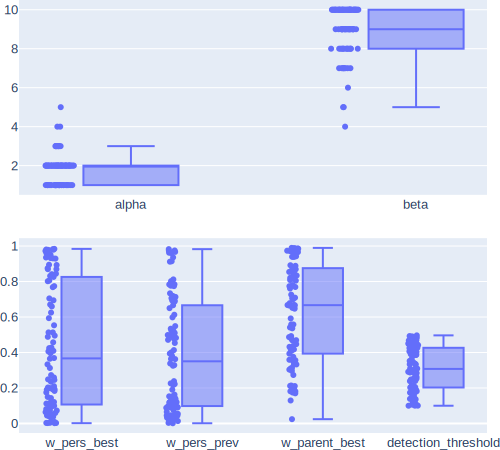
\includegraphics[width=0.85\textwidth]{results/part2/parameter_boxplot_None.svg}
	\caption[Statistical box plot of \gls{hsppbo} parameters]{Statistical box plot of all \gls{hsppbo} parameters (except $H$) over all 90 optimizer runs.}
	\label{fig:parameter_boxplot}
\end{figure}

Starting with the box plot, which is not grouped by any metric, \cref{fig:parameter_boxplot} shows, in addition to the information already described, all 90 values for each parameter as scattered dots next to the box itself. The results for $\alpha$ suggest that it is the most robust parameter of the six, with the median falling together with the upper quartile at 2, and the minimum and lower quartile sharing their value at 1. A value of $\gls{iqr} = 1$ is remarkably low and can only be improved later on in the analysis, when looking at aggregated box plots. The \gls{gbrt} surrogate model seemed to have no problem finding appropriate values for $\alpha$, and since a value of zero was never chosen, a floor effect can be ruled out. The $\beta$ shows a much larger spread around its median of 9 and has a very low fence of 5. However, its \gls{iqr} of 2 suggests that the \gls{hpo} process was mostly consistent in finding values for this parameter. The abrupt end of the upper quartile and the maximum at 10 suggests a ceiling effect (see \cref{chap:choice-param}), which was supposed to be avoided by a sufficiently large value range. Apparently, an upper limit of 10 was not enough for $\beta$. However, since at least 50\% of the values are at or below 9, this effect should not have had a significant influence on the choice of this parameter during \glsdesc{hpo}. 

The three weights, $w_{\text{persbest}}, w_{\text{persprev}}$, and $w_{\text{parentbest}}$, on the other hand, show considerably high dispersion. In particular, the box plot for $w_{\text{persbest}}$ has an $\gls{iqr} = 0.72$, which is almost as large as the possible value range from 0 to 1, with the whiskers reaching these boundaries. Therefore, the median of 0.37 has almost no significance in choosing an optimal parameter based on means alone. This situation improves slightly when looking at the remaining two weights. Although their box plots also span the entire value range, their \gls{iqr} is at about half of the range ($\gls{iqr}_\text{persprev} = 0.57, \gls{iqr}_\text{parentbest} = 0.48$). Therefore, the medians of $w_{\text{persprev}}$ at 0.35 and of $w_{\text{parentbest}}$ at 0.66 can both be considered somewhat robust. However, the fact that all three of these weights are used together in a sum makes any value suggestion an almost random one. Only the absolute parameter configuration range between 0 and 1 and a vague specification of this range for the latter two weights can be confirmed to some extent.

The box plot for the dynamic detection threshold $\theta$ shares its y-axes with the three weights, but only has a possible value range between 0.1 and 0.5. Therefore, its \gls{iqr} is quite large at 0.22 or more than half of its range. The same dispersed behavior can be seen with its whiskers, which reach their minimum and maximum values almost exactly to the third decimal point. Without any kind of grouping applied to the data, no recommendation can be given for the detection threshold and regarding the \gls{hpo} process, this parameter could not be chosen reliably.

\begin{figure}[h]
	\centering
	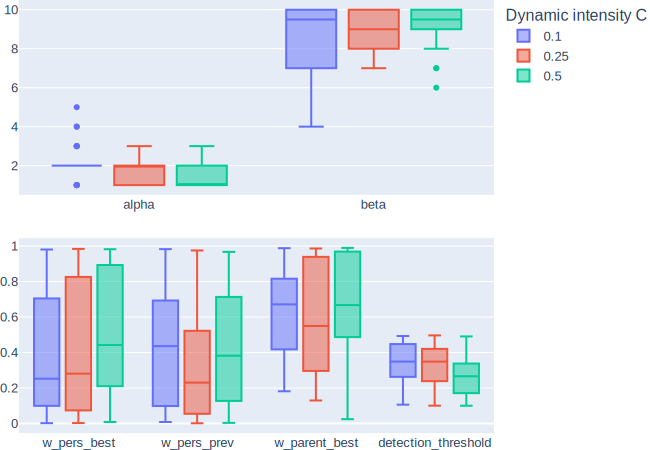
\includegraphics[width=\textwidth]{results/part2/parameter_boxplot_dynamic.svg}
	\caption[Statistical box plot of \gls{hsppbo} parameters compared by dynamic intensity]{Statistical box plot of all \gls{hsppbo} parameters (except $H$) over all 90 optimizer runs and compared by dynamic intensity $C$.}
	\label{fig:parameter_boxplot_dynamic}
\end{figure}

Continuing with the box plots shown in \cref{fig:parameter_boxplot_dynamic}, where the data points are grouped by the three dynamic intensities $C$ tested, an interesting trend emerges for $\alpha$ and $\beta$. For a low dynamic intensity, i.e. very few cities swap places every $T_d = 100$ iterations, an $\alpha$ value of exactly 2 seems to be the ideal choice for the \gls{hpo} process, with an \gls{iqr} of 0 and only four outliers in total. Parameter $\beta$, on the other hand, shows a similarly low dispersion for the highest dynamic of $C = 0.5$. With an $\gls{iqr} = 1$ and a median of 9.5, a strong heuristic influence seems to be beneficial in obtaining good solutions in highly dynamic problems. In the case of $\alpha$, the other two higher dynamics introduce more spread in the choice of values, but always remain in a median range between 1 and 2, with a small dispersion of 1. For $\beta$, the robustness decreases significantly with lower dynamic intensity, reaching a high $\gls{iqr} = 3$ for $C = 0.1$.

As with the ungrouped box plots, the three weights show no sign of robust value behavior. Although small improvements can be observed for certain weights under certain dynamic intensities, e.g., $w_{\text{parentbest}}$ has a comparatively low dispersion of $\gls{iqr} = 0.4$ and a reduced minimum for $C=0.1$, the spread is still far too large to provide any value suggestions under certain dynamic environments. 
Aside from the robustness, the two personal weights, $w_{\text{persbest}}, w_{\text{persprev}}$, have a particularly different median for the lowest dynamic of $C=0.1$, although the medians for the other dynamic intensities are quite similar. This may be due to the fact that, especially in a low dynamic environment the populations for both personal weights become equal after a certain number of \gls{hsppbo} iterations. Therefore, a reset of the personal best population (whether partial or full) still gives the \gls{sce} a copy of that solution through the personal previous solution, which then influences that weight to be more important during \gls{hpo}.

The same statements about robustness can be made for the dynamic threshold $\theta$, where an improvement in the \gls{iqr} of about 0.05, which is 12.5\% of its value range, still does not allow for a sophisticated parameter choice. The only hinted trend might be, contrary to intuition, that lower values of $\theta$, i.e. less \gls{sce} tree swaps necessary to trigger the change handling procedure, benefit solving higher dynamic problem instances ($C=0.5$). However, with a median of 0.27, the upper quartile region still completely overlaps with the other two groups.

\begin{figure}[h]
	\centering
	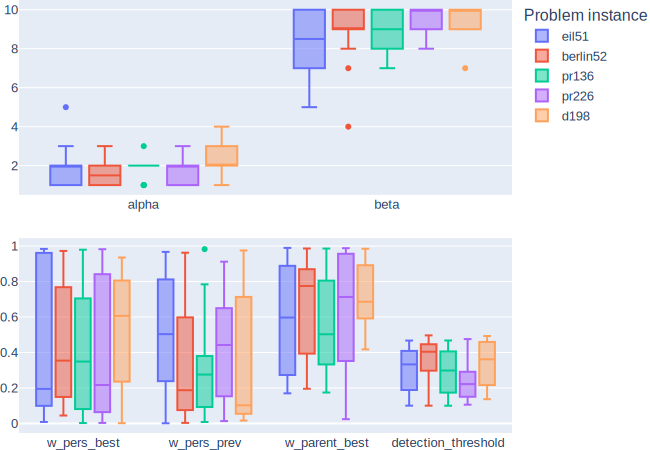
\includegraphics[width=\textwidth]{results/part2/parameter_boxplot_problem.svg}
	\caption[Statistical box plot of \gls{hsppbo} parameters compared by problem instance]{Statistical box plot of all \gls{hsppbo} parameters (except $H$) over all 90 optimizer runs and compared by problem instance.}
	\label{fig:parameter_boxplot_problem}
\end{figure}

\Cref{fig:parameter_boxplot_problem} shows the parameter box plots grouped by the \gls{tsp} problem instance on which they were acquired on. The parameter $\alpha$ shows a low dispersion for \texttt{pr136}, an instance with a moderately clustered structure, and an unusually high dispersion for \texttt{d198}, an instance with highly clustered areas. The other problem instances show similar results as before, and the median for all five instances is still between 1.5 and 2. The same conclusions can be drawn for $\beta$, where the instances \texttt{berlin52, pr226}, and \texttt{d198} show low \glspl{iqr} of 2, while the remaining two instances, especially \texttt{eil51}, show very unreliable values with medians as low as 8.5. 

The three weights show very dispersed distributions, as expected from previous observations, with \texttt{eil51} probably being the most spread out of all values. Only some instances have an improving effect on the robustness, e.g. $w_{\text{persprev}}$ for instance \texttt{pr136} with a low $\gls{iqr} =  0.29$ and a median of 0.28, or $w_{\text{parentbest}}$ for instance \texttt{d198} with $\gls{iqr} =  0.30$ and a median of 0.69. Also, compared to the values from the previous figures, $w_{\text{parentbest}}$ seems to be much more robust across all instances (except \texttt{pr226}), suggesting that this value could be very dependent on the particular problem it is used for.
The detection threshold $\theta$ shows in some instances, i.e. \texttt{berlin52} and \texttt{pr226}, a more robust value selection with \glspl{iqr} around 0.15, which is even better, than the aggregation by dynamic intensity shows. However, these two robust values are very different, with medians of 0.40 and 0.22, respectively, suggesting that dynamic detection may be strongly influenced by the problem instance on which it is used on. This is also seen in the data for the reaction type $H$, which is discussed in the following.
 
\begin{table}[h]
	\centering
	\caption[The distribution of the \gls{hsppbo} reaction type $H$]{The distribution of the \gls{hsppbo} reaction type $H$. Either for all parameter sets or for parameter sets grouped by dynamic intensity $C$ or problem instance, the percentages of these sets using one or the other reaction type are given.}
	\label{tab:reaction-type}
	
	\begin{tabular}{ccS[table-omit-exponent, fixed-exponent = -2, round-precision = 1]S[table-omit-exponent, fixed-exponent = -2, round-precision = 1]}
		\hline
		Comparison & Group & $H_\text{partial}$ [\si{\percent}] & $H_\text{full}$ [\si{\percent}] \\ \hline
		- & - & 0.6666666666666666 & 0.3333333333333333 \\  \hline
		\multirow{3}{*}{Dynamic Intensity} & 0.1 & 0.7666666666666667 & 0.23333333333333334 \\ 
		& 0.25 & 0.5666666666666667 & 0.43333333333333335 \\ 
		& 0.5 & 0.6666666666666666 & 0.3333333333333333 \\ \hline
		\multirow{3}{*}{\shortstack{Dynamic Intensity\\Best 50\% RPD}} & 0.1 & 0.6666666666666666 & 0.3333333333333333 \\ 
		& 0.25 & 0.5333333333333333 & 0.4666666666666667 \\ 
		& 0.5 & 0.6666666666666666 & 0.3333333333333333 \\ \hline
		\multirow{5}{*}{Problem Instance} 
		& eil51 & 0.6111111111111112 & 0.3888888888888889 \\ 
		& berlin52 & 0.7222222222222222 & 0.2777777777777778 \\ 
		& pr136 & 0.7777777777777778 & 0.2222222222222222 \\ 
		& pr226 & 0.8333333333333334 & 0.16666666666666666 \\
		& d198 & 0.3888888888888889 & 0.6111111111111112 \\  \hline
		\multirow{5}{*}{\shortstack{Problem Instance\\Best 50\% RPD}} 
		& eil51 & 0.5555555555555556 & 0.4444444444444444 \\ 
		&  berlin52 & 0.6666666666666666 & 0.3333333333333333 \\ 
		& pr136 & 0.6666666666666666 & 0.3333333333333333 \\ 
		& pr226 & 0.7777777777777778 & 0.2222222222222222 \\ 
		& d198 & 0.4444444444444444 & 0.5555555555555556 \\ \hline
	\end{tabular}
\end{table}

The dynamic reaction mechanism $H$ was chosen to be discussed separately, because a two-valued categorical value is not effectively represented by a box plot. Instead, \cref{tab:reaction-type} shows the distribution across the same comparison groups as used in the box plots. In addition to the two grouped versions, distributions for only those parameter sets that resulted in 50\% or better relative solution qualities ($RPD$) were added to represent what values the best parameter sets use for $H$.

It is immediately evident that the partial reaction $H_\text{partial}$ is most often preferred by the \glsdesc{hpo}, except for some deviations. In the overall (ungrouped) comparison, twice as many parameter sets used this method of dynamic reaction. For the lowest ($C=0.1$) and highest ($C=0.5)$ dynamic intensities, this preference can also be confirmed, while for medium intensity, $H_\text{full}$ is also a viable choice 43.3\% of the time. Except for a slight percentage decrease for $H_\text{partial}$ with $C=0.1$, this behavior does not change for the best 50\% of solutions.
When grouped by \gls{tsp} instance, the only problem that does not favor a partial reset appears to be \texttt{d198}, where 61.1\% of the parameter sets use the $H_\text{full}$ method. Contrary to this observation, the \gls{hpo} process chose the partial reset 83.3\% of the time for \texttt{pr226}, which is the highest bias toward any $H$ method. Looking at the best 50\% of parameter sets, \texttt{eil51} clearly deviates from any preference and has both methods almost at 50\%. The other instances also show a decrease in their bias towards $H_\text{partial}$, except for \texttt{d198}, which now seems to choose the full reset less often for its better solutions.

\subsubsection{Parameter Value Recommendations}
\label{chap:param-recommend}

Based on the previous discussion of parameter robustness, their median values, and possible preferences and trends with respect to certain combinations of dynamic intensity and problem instance, some general recommendations for potentially well-performing parameter sets are given. These suggested value ranges could be used to refine the \gls{hpo} parameter configuration or as guidelines for manual parameter tuning.

Starting with the two most robust recommendations, $\alpha$ and $\beta$, which had the lowest \glspl{iqr} out of all parameter box plots. The median for $\alpha$ was almost always at 2, with boundaries rarely exceeding the interval $[1,2]$. This was also the parameter that was least affected by a change in the problem description, making the choice of $\alpha = 2$ the most robust suggestion. The parameter $\beta$ usually had a median between $[9,10]$ and is slightly influenced by dynamic intensity and problem instances. Since in some combinations $\beta$ was chosen as low as 4, with a lower quartile value of around 7, and considering the ceiling effect, a value range between $[7,12]$ might lead to satisfactory solutions.

The dynamic reaction type $H$ was also most often chosen as $H_\text{partial}$. The influence of different dynamic intensities also seems to be marginal, since only the medium dynamic ($C=0.25$) leads to a change in the distribution, with the highest and lowest tested values still favoring the partial reset. This also holds true for the problem instances, where the results only suggest that certain city placement characteristics - very regular instances like \texttt{eil51} (group 1) or highly clustered instances like \texttt{d198} (group 5) - might have an influence on this choice. Nevertheless, the data indicates that the $H_\text{partial}$ method is the preferred option.

The three weights, $w_{\text{persbest}}, w_{\text{persprev}}$, and $w_{\text{parentbest}}$, are not only agnostic to varying dynamic intensities and problem instances, but their choice also seems to be influenced by some other, possibly random, relationship. Regardless, their median values may still be useful as a symptom of the underlying well-performing parameter sets. The parameter $w_{\text{persbest}}$ has a median between 0.28 and 0.44, and is only influenced by higher dynamics ($C=0.5$) and certain, highly clustered, problem instances (\texttt{d198}). On the other hand, $w_{\text{persprev}}$ seems to be strongly influenced by dynamic intensity and problem instance, resulting in a median between 0.10 and 0.50. And $w_{\text{parentbest}}$, which has the lowest \gls{iqr} of the three, has its median range between 0.50 and 0.78, showing a slight dependence on dynamic intensity and a stronger influence from problem instances. Also, since this range is above the other two weights, it could be implied that the parent-best population might be slightly more significant to the solution construction procedure. These three median ranges can be used as value range suggestions and at least somewhat confirm the \gls{hpo} configuration range between 0 and 1, with no strong floor or ceiling effect present in the data.  

Finally, the detection threshold $\theta$ was slightly influenced by the dynamic intensity, with an interesting preference towards lower values of 0.27 for highly dynamic intensities of $C=0.5$, and was strongly influenced by problem instances. Again, the configured \gls{hpo} value range between 0.1 and 0.5 was confirmed in terms of the lower and upper quartiles never getting too close to these boundaries. However, the high median interval for the problem aggregated statistic of $[0.22, 0.40]$ still spans half of the available range, with the advantage that this suggestion still narrows the range.

In summary, the following parameter range configuration can be seen as a possible refinement to the one given in \cref{chap:choice-param} to reduce the number of objective calls needed to find good parameter sets using \gls{hpo} with \gls{gbrt} for the \gls{hsppbo} metaheuristic, regardless of dynamic intensity or \gls{tsp} problem instance:
\begin{itemize}
	\item $\beta \in \left\lbrace x\in\mathbb{N} | 7 \leq x \leq 12 \right\rbrace$
	\item $w_{\text{persprev}} \in [0.10,0.50]$
	\item $w_{\text{persbest}} \in [0.28,0.44]$
	\item $w_{\text{parentbest}} \in [0.50,0.78]$
	\item $\theta \in [0.22,0.40]$
	\item $H = H_{\text{partial}}$ (not optimized)
	\item $\alpha = 2$ (not optimized) 
	\item $L_\text{pause} = 5$ (not optimized)
\end{itemize}
 In addition, this configuration should further speed up the optimization process and may even increase the quality of the solutions found by reducing the dimensions of the configuration space.

\subsection{Parameter Interaction and Influences}

Besides the analysis of the parameter robustness, another point of interest is the parameter interaction, not only among themselves, but also with respect to certain dynamic intensities.
For this purpose, scatter matrix plots were generated showing every possible combination of two \gls{hsppbo} parameters on the x- and y-axis, respectively, with an optional aggregation over dynamics. Since the resulting matrix would have been antisymmetric, the upper right triangle was omitted to improve readability. The resulting assignment of a parameter to a particular axis, rather than showing the opposite paring as well, does not reflect any real dependence of one parameter on another. As with the previous box plots, the reaction type $H$ was excluded not only for lack of information gain, but also to reduce the size of the matrix and make the figure legible on paper. When analyzing the scatter plots, the ungrouped and dynamic-aggregated figures are used together for each parameter pairing, rather than being discussed one after the other.

\begin{figure}[h]
	\centering
	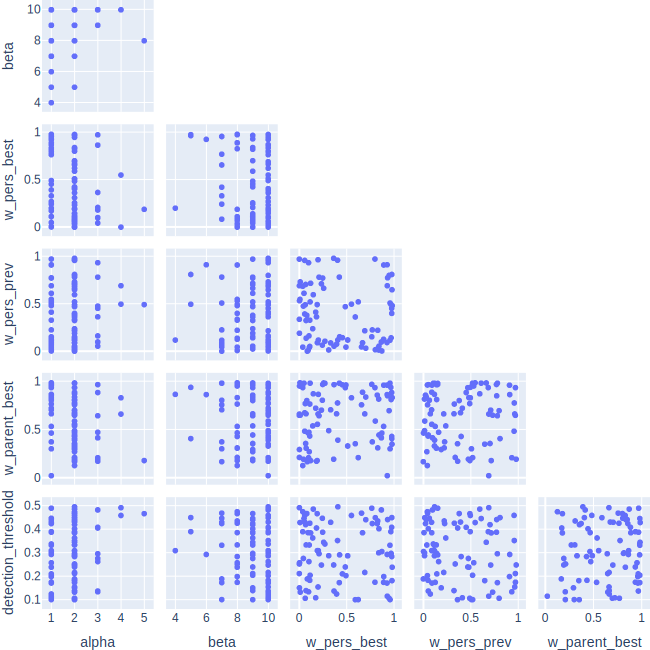
\includegraphics[width=\textwidth]{results/part2/param_scatter_matrix_None.svg}
	\caption[Scatter matrix plot of all \gls{hsppbo} parameters]{Scatter matrix plot of all \gls{hsppbo} parameters (except $H$) over all 90 optimizer runs.}
	\label{fig:parameter_scatter_matrix}
\end{figure}

\begin{figure}[h]
	\centering
	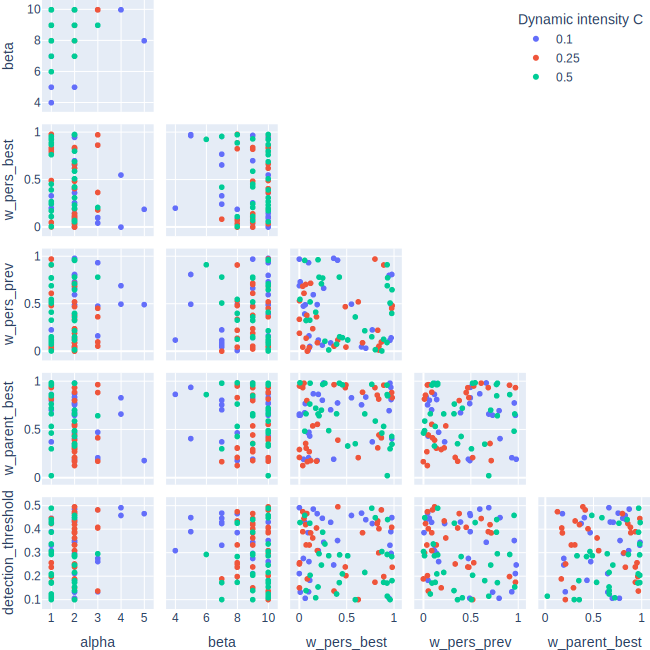
\includegraphics[width=\textwidth]{results/part2/param_scatter_matrix_dynamic.svg}
	\caption[Scatter matrix plot of all \gls{hsppbo} parameters compared by dynamic intensity]{Scatter matrix plot of all \gls{hsppbo} parameters (except $H$) over all 90 optimizer runs and compared by dynamic intensity $C$.}
	\label{fig:parameter_scatter_matrix_dynamic}
\end{figure}

Starting with the ungrouped scatter matrix, \cref{fig:parameter_scatter_matrix}, and looking at the first parameter pairing, with values for $\alpha$ on the x-axis and values for $\beta$ on the y-axis, we can see an interesting distribution towards the upper left corner of the plot. This suggest a correlation, with higher $\beta$ values, between 8 and 10, allowing for higher $\alpha$ values, between 2 and 4. This confirms the relationship between these two parameters for many other metaheuristic parameter tuning procedures as well. However, some parameter sets with high $\beta$ values between 8 and 10, also found small $\alpha$ values of 1 to produce favorable solutions. Furthermore, the region of high values for $\alpha$ and low values for $\beta$ seems to be of little interest for good parameter sets. 

\Cref{fig:parameter_scatter_matrix_dynamic} shows yet another probable correlation due to the influence of different dynamics. In the case of overlapping points, the color of the dynamic intensity was displayed, which is the most common for this parameter combination.
For $\alpha$ and $\beta$, interesting enough, the previously preferred combination of high values of $\beta$ allowing higher values of $\alpha$ most often applies to low dynamic intensities of $C=0.1$, while the opposite correlation, $\beta \in [4,5]$ and $\alpha = 1$, is also used for this dynamic. For the highest dynamic intensity of $C=0.5$ the values for $\alpha$ were not chosen as high with increasing $\beta$, implying that the heuristic influence is relatively more important than the stochastic solution construction for highly dynamic problems.

Continuing down one row, we have $w_{\text{persbest}}$ being paired with $\alpha$ and $\beta$. First, for $\alpha=1$ there is an unusual, but significant gap for the value of $w_{\text{persbest}}$ between 0.5 and 0.75, which increases even further for $\alpha=3$, but inexplicably disappears for $\alpha=2$. Similar gaps in the choice of values can also be found for $\beta = 8$. In the case of the dynamic comparison, no further trend can be found in the scatter plots, except for the value choices already discussed in the previous subsection.

For $w_{\text{persprev}}$, there are only value gaps for $\alpha = 3$ and $\beta = 8$. Especially for the pairing with $\beta$, there is a slight trend towards smaller values for $w_{\text{persprev}}$ for smaller $\beta$ values, with an interesting area for the lowest dynamic intensity of $C=0.1$ and a $\beta = 7$ using unusually low values for $w_{\text{persprev}}$ between 0 and 0.2. The combination of $w_{\text{persprev}}$ and $w_{\text{persbest}}$ shows a significant avoidance of a medium-value area where both parameters are around 0.5, with only four exceptions. Therefore, it is implied that these two parameters are preferred in pairings near the value boundaries, with a small bias towards a low-low-combination. In particular, for a medium dynamic environment of $C=0.25$, lower values for $w_{\text{persprev}}$ below 0.2 are most often used with similarly low values for $w_{\text{persbest}}$.

The parameter $w_{\text{parentbest}}$ shows no clear trend when interacting with $\alpha$ or $\beta$. As with the interaction between the other two weights, the pairing with both $w_{\text{persprev}}$ and $w_{\text{persbest}}$ shows the same avoided mid-area around values of 0.5 for both parameter, although not as pronounced. The bias towards higher values for $w_{\text{parentbest}}$ above 0.2, especially at low dynamic intensities, can also be seen in these scatter plots. Another interesting area to note is present in the pairing with $w_{\text{persprev}}$, where a clear notch in the distribution is visible for $w_{\text{parentbest}} \in [0.8,1]$ and $w_{\text{persprev}} \in [0.2,0.5]$. However, this does not justify an indication of a possible correlation and could just be a random influence. 

Finally, the detection threshold $\theta$ is paired with all other parameters. With $\alpha = 2$, there is a preference for smaller values of $\theta < 0.3$ for high dynamic intensities of $C=0.5$. The opposite can be observed at low dynamics of $C=0.1$ with smaller $\beta \leq 7$ that are being paired with $\theta$ values greater than 0.3. The interaction with any of the three weights does not show any obvious correlation or tendency towards certain areas.

For completeness, \Cref{fig:parameter_scatter_matrix_added} in \cref{chap:figures} also shows the ungrouped version of the scatter plot that includes the dynamic reaction parameter $H$. However, other than avoiding the full reset method ($H_\text{full}$) for low detection threshold $\theta$ values between 0.1 and 0.15, nothing noteworthy is added by this matrix.

In conclusion, only the interaction between $\alpha$ and $\beta$ seems to suggest some kind of correlation between these parameters. In particular, since $\alpha$ is used as an exponent for the sum of the three weights, one might expect some kind of relationship between these parameters. But even when $\alpha$ was plotted in a semi-logarithmic scatter plot over the sum of all three weights (see \cref{fig:alpha_weight_semilog_plot}), no particular distribution became apparent. Therefore, at least for this specific case of \gls{hpo} using \gls{gbrt}, there does not appear to be a direct relationship between these parameters. The same can be said for any other combination of parameters where no zero-order correlation is apparent. However, a higher order correlation across multiple parameters may still be possible and could be further investigated with a different test setup that also samples parameter areas that lead to sub-optimal solutions, i.e., that is not driven by \gls{hpo} goals.


\subsubsection{Partial Dependence}

Although we have already discussed the abundance of strong correlations between parameter pairings, the following partial dependence plots, as described in \cref{chap:an-part2}, take advantage of the predictive capabilities of the final surrogate model generated during \gls{hpo}. Since each of the 90 optimizer runs produced one model, only the model with the best solution quality was used, following the same reasoning as for the selection of the optimal parameter sets described at the beginning.

For each parameter (dimension), 60 points were evaluated across their value ranges, with each point averaged over 250 prediction samples. In the one-dimensional case, shown in the diagonal line plots, this allows for an analysis of the effect of a single dimension on the predicted objective function, i.e., which parameter values most affected the output of the surrogate model. In the two-dimensional case shown below the diagonal, this effect is shown for a combination of two parameters using contour plots. Light colored (yellow) areas represent better solutions (smaller prediction for tour length $L$), while dark colored (blue) areas represent worse solution areas. The black dots represent the observed points during the \gls{hpo}, and the red star in each contour plot marks the best observed parameters. Due to the qualitative nature of these visualizations, and since this is only a strong estimate of what might be really important for the actual \gls{hsppbo} metaheuristic, no explicit quantitative color-map is used, and the $PD$ values on the diagonal one-dimensional plots are to be understood only as relative orientation.

Due to the size of these partial dependence plots, not all 15 possible figures are shown in the following, but only the two most interesting ones, showing the results for the problem instance \texttt{berlin52} and for dynamic intensities $C={0.25,0.5}$, are discussed. However, these two chosen figures are most representative, especially in the context of the analysis from previous subsections, and necessary remarks for the other unused figures will be included if necessary. These other 13 figures are also available in the GitHub repository of this thesis.

\begin{figure}[h!]
	\centering
	\centerline{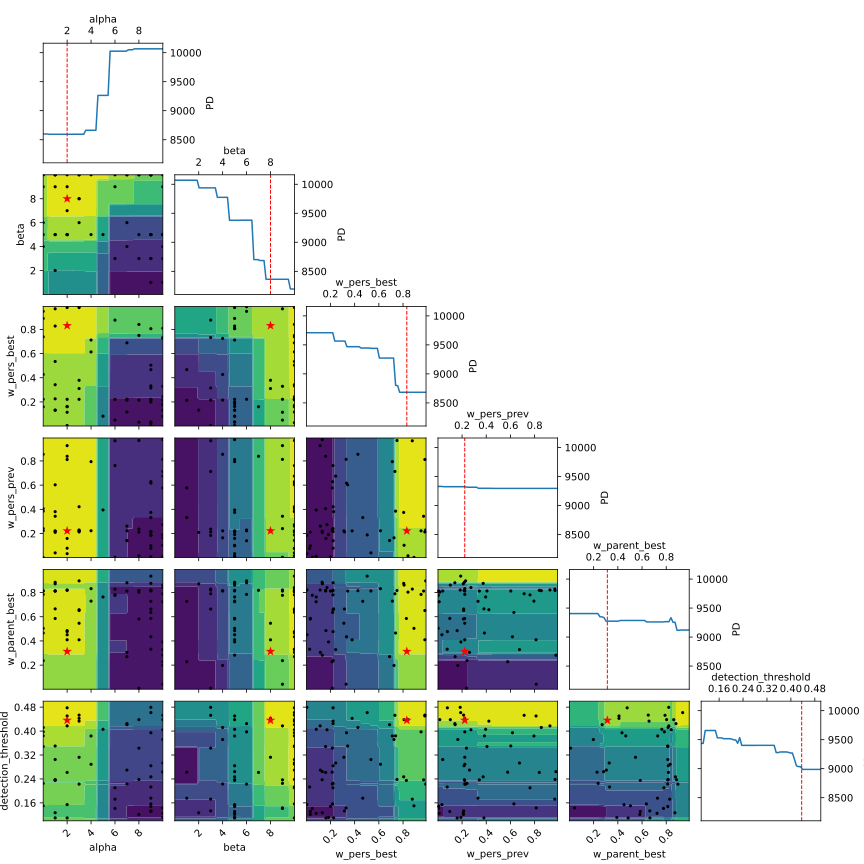
\includegraphics[width=1.2\textwidth]{results/part2/partial_dependence_berlin52_C_0.25_run_4.svg}}
	\caption[Partial dependence plot for \texttt{berlin52} and $C=0.25$]{Partial dependence plot using the surrogate model of the optimizer run with the best parameter set for problem instance \texttt{berlin52} and dynamic intensity $C=0.25$. Better (smaller) solutions are lightly colored, dark areas represent worse solution areas.}
	\label{fig:partial_dependence_berlin52_C_025}
\end{figure}

\Cref{fig:partial_dependence_berlin52_C_025} shows the partial dependence for $C=0.25$. Starting from the diagonal, a low value for $PD$, i.e. a good solution quality, was obtained by the model for $\alpha$ values between 1 and 4, with a steep edge around $\alpha=5$. The solution quality also seems to improve dramatically for higher values of $\beta$, with $\beta \geq 8$ as the optimum. The resulting combination of the two, shown in the contour plot to the left and below these two one-dimensional plots, confirms similar value areas as described previously in \cref{fig:parameter_scatter_matrix}, where the light-colored, good areas are in the upper left corner of the plot, i.e., the high $\beta$, low $\alpha$ value range. The opposite dark blue corner also confirms that this area of high values for $\alpha$ and low values for $\beta$ also leads to predicted bad solutions for the model, which is why this area was never part of a good parameter set. This observation for $\alpha$ and $\beta$ can be made for almost all of the other 14 partial dependence plots, with the only difference that $\alpha$ sometimes has significantly less influence on a good solution, resulting in the contour plot suggesting good solutions for any $\alpha$ value paired with $\beta \geq 8$.

Continuing on the diagonal, high values for $w_{\text{persbest}}$ seem to have a large impact on the solution quality for the predictive model, with $w_{\text{persbest}} > 0.8$ as the optimum. Interestingly, this result differs greatly from previous observations from the statistical box plots grouped by problem instance, where \texttt{berlin52} had a median of 0.35. The contour plots also show clear preferences for high values of $w_{\text{persbest}}$ in combination with high values of $\beta$ and especially with low values of $\alpha$.

On the other hand, the model predicts the same $PD$ regardless of any value of $w_{\text{persprev}}$. This is also evident in the contour plots of the same row, where the light-colored good solution areas are only affected by well-performing $\alpha$ and $\beta$ values, respectively. This is also true for the combination of $w_{\text{persbest}}$, where the avoided area shown in the scatter matrices is also absent.

The parameter $w_{\text{parentbest}}$ has a small influence on the model prediction, with values $ > 0.85$ being most beneficial for a low $PD$. However, this influence does not appear to be sufficient when looking at the contour plots for the first three parameters from the left, where a similarly distinct edge can be seen that is mainly influenced by these more influential parameters. In combination with $w_{\text{persprev}}$, almost no area seems to be of real interest except for a narrow region in the upper right, suggesting that the previously mentioned high values for $w_{\text{parentbest}}$ should be paired with also high values for $w_{\text{persprev}}$.

The detection threshold $\theta$ showed its lowest value for $PD$ at $\theta > 0.44$. This value range is also seen in the contour plots, where the light-colored areas are always above 0.4, except in combination with $\beta$ values close to 10, where lower values for $\theta$ are also possible, suggesting that the higher heuristic influence could compensate for scarcer dynamic detection and thus triggered dynamic reaction mechanisms. 
Furthermore, by looking at the red stars, we can see that the \gls{hpo} process almost always chose a parameter in the areas favored by the surrogate model, except for the pairing of $w_{\text{persprev}}$ and $w_{\text{parentbest}}$, where the predicted best, yellow area in the upper right corner, was never even sampled by the aggregation function.

\begin{figure}[h!]
	\centering
	\centerline{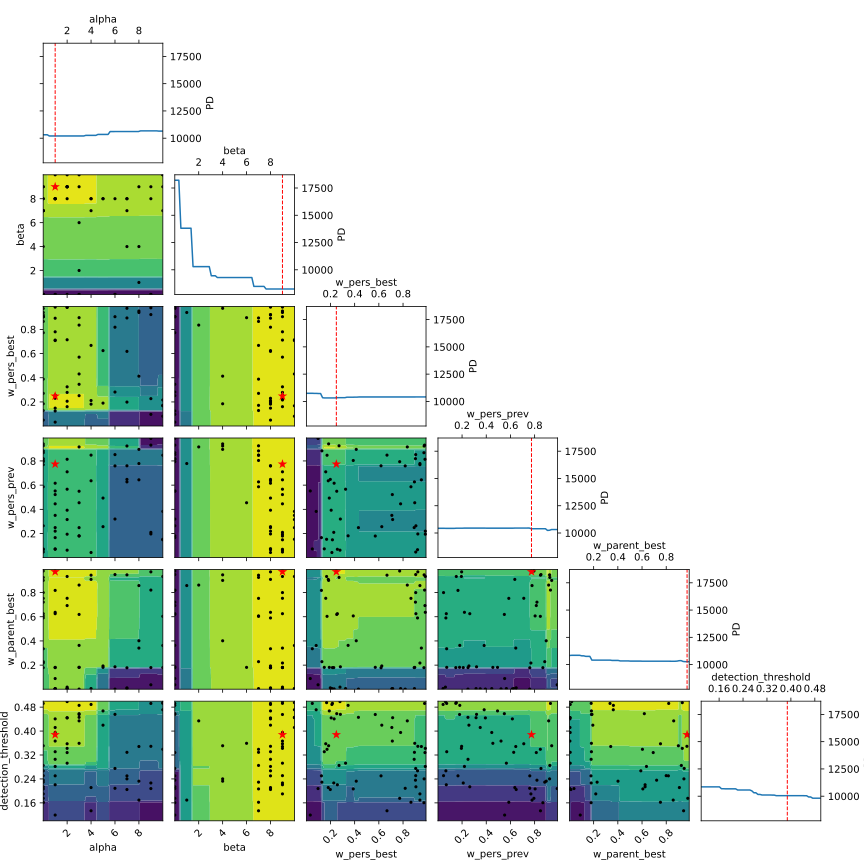
\includegraphics[width=1.2\textwidth]{results/part2/partial_dependence_berlin52_C_0.5_run_4.svg}}
	\caption[Partial dependence plot for \texttt{berlin52} and $C=0.5$]{Partial dependence plot using the surrogate model of the optimizer run with the best parameter set for problem instance \texttt{berlin52} and dynamic intensity $C=0.5$. Better (smaller) solutions are lightly colored, dark areas represent worse solution areas.}
	\label{fig:partial_dependence_berlin52_C_05}
\end{figure}

The second partial dependence plot, \cref{fig:partial_dependence_berlin52_C_05}, shows the results for a higher dynamic intensity of $C=0.5$. 
The same results hold for $\alpha$ and $\beta$, but with the aforementioned lesser influence of smaller $\alpha$ values on $PD$ in the one-dimensional plot. The diagonal plot for $\beta$ also shows a less significant decrease in $PD$ between 4 and 8 than before, instead resembling more of an exponential function. The weight $w_{\text{persbest}}$ is also much less influential for the surrogate model. In fact, the diagonal plots for all three weights show that no particular value in the entire range between 0 and 1 has a significant impact on the prediction of the surrogate model, at least compared to $\beta$. This is also true for the detection threshold $\theta$. The corresponding contour plots for the weights and $\theta$ show similar edges, separating light-colored good solution areas from darker areas, as with $C=0.25$, but with less intense dark-colored spots, suggesting that more areas could result in satisfactory performance. The remaining 13 partial dependence plots show very similar results for the weights and $\theta$.

In addition, compared to the previous, less dynamic representation of the partial dependence, the best observed parameters, indicated by the red stars, are less often in the areas indicated as optimal by the model, suggesting a mismatch between \gls{hpo} and the produced model. In this case, potentially more objective calls or a reduction of the parameter dimension could improve this situation. However, it is quite possible that this mismatch is only produced by the random sampling of the model prediction and is not significantly present in repeated predictions with a different random initialization.

Concluding, we can confirm some relationships between parameters, especially that of $\alpha$ and $\beta$. However, even by using the trained model for its predictive capabilities, we did not gain any further insight into possible direct correlations between parameters. Nevertheless, the importance of certain parameters for the surrogate model is an interesting addition to this analysis.

\subsection{Parameter Importance}
\label{chap:param-importance}

In the previous subsection, regarding the partial dependence plots, we already discussed the influence of the parameters on the surrogate model and its prediction of solution quality. This was achieved by explicitly sampling the parameter search space using the surrogate model. For some simpler \gls{ml} models, mostly decision tree-based, the feature, or in this case the parameter importance, can be  extracted directly from the structure of the model. The previously required intermediate sampling is now replaced by analyzing the structure of the regression trees of the \gls{gbrt} surrogate model used for the experiments. The resulting relative parameter importance, or so-called \glsfirst{mdi}, as explained in \cref{chap:an-part2}, expresses how important a particular parameter is for the prediction of the underlying model. For example, for a simple linear regression, $y = a_0  \cdot x_1 + a_1 \cdot x_1 + ... + a_n \cdot x_n$, the values for $a_i$ would indicate the relative importance for their corresponding parameter $x_i$. 

As mentioned earlier in the experimental setup chapter, the procedure for calculating the \gls{mdi} has some limitations. It has a bias towards parameters with high cardinality and therefore tends to underestimate the importance of parameters such as $H$, which has only two values. Furthermore, it can only reflect the importance resulting from the 60 objective calls during the optimizer run, i.e., it is not a statement about the importance of the entire parameter search space and, as such, of the \gls{hsppbo}. Nevertheless, the \gls{mdi} is still an indicator of what the model considered important enough to base its predictions on, which then guides the successful search for well-performing parameter sets. 

\begin{table}[h]
	\centering
	\caption[Relative parameter importance over all 90 optimizer runs]{The relative parameter importance (\gls{mdi}) computed via the surrogate model over all 90 optimizer runs with the standard error. }
	\label{tab:parameter_importance}
	\begin{tabular}{cccc}
		\hline
		$\beta$ & $\alpha$ & $w_{\text{parentbest}}$ & $\theta$ \\ \hline
		  \num{0.3026887387214929} $\pm$ \num{0.0068271325972591185} & 
		  \num{0.18503797670261257} $\pm$ \num{0.005773445553779512} & 
		  \num{0.13219322556428054} $\pm$ \num{0.0048906270152243485} & 
		  \num{0.1316600435540604} $\pm$ \num{0.005210027993794393} \\ \hline
	\end{tabular}
	\bigskip\\
	\begin{tabular}{ccc}
		\hline
		$w_{\text{persprev}}$ & $w_{\text{persbest}}$ & $H$ \\ \hline
		\num{0.11494569405569222} $\pm$ \num{0.004096682063210092} & 
		\num{0.10821824956197788} $\pm$ \num{0.003648963763332609} & 
		\num{0.025256071839883553} $\pm$ \num{0.0023011990335138335} \\ \hline
	\end{tabular}
\end{table}


\cref{tab:parameter_importance} shows the averaged \gls{mdi} for all \gls{hsppbo} parameters with their standard errors over all 90 optimizer runs. The table is also ordered from the most highest value (left) to the lowest value (right), and all values sum to 1. The importance of the parameter $\beta$ is by far the highest at 0.303, indicating that about a third of each model-prediction is explained by this value. The standard error is also the highest by comparison, but still very low and far away from the margin of error for the second most important parameter, $\alpha$, at 0.185. This difference of more than 10\% between the first and second most important parameters suggests that although this \gls{mdi} metric is biased, $\beta$ is definitely an important parameter for the \gls{hsppbo} metaheuristic. Including the importance of $\alpha$ may also explain why only these two parameters were the most robust and consequently allowed for a reasonably meaningful value suggestion.

The next most important parameters are $w_{\text{parentbest}}$ and $\theta$, both with $\gls{mdi} = 0.132$, also with very low standard errors when averaged over all optimizer runs. In particular, $w_{\text{parentbest}}$ showed a slightly more robust behavior in the box plots and also had a higher median than the other two weights, thus implying more importance to the solution creation process. Therefore, it seems reasonable that $w_{\text{parentbest}}$ has a higher \gls{mdi} than the other weights.

This is followed by $w_{\text{persprev}}$ at $\gls{mdi} = 0.115$ and $w_{\text{persbest}}$ at $\gls{mdi} = 0.108$, both of which are very close to the previous two parameters, with at most 3\% less importance. Their standard errors are also very small, at around 3.5\% relative to their values. The least important parameter, as already indicated by the bias, is the dynamic reaction type $H$. With only $\gls{mdi} = 0.025$, it is four times less important than the next most important parameter $w_{\text{persbest}}$ and 12 times less important than the most relevant parameter $\beta$.

\begin{figure}[h!]
	\centering
	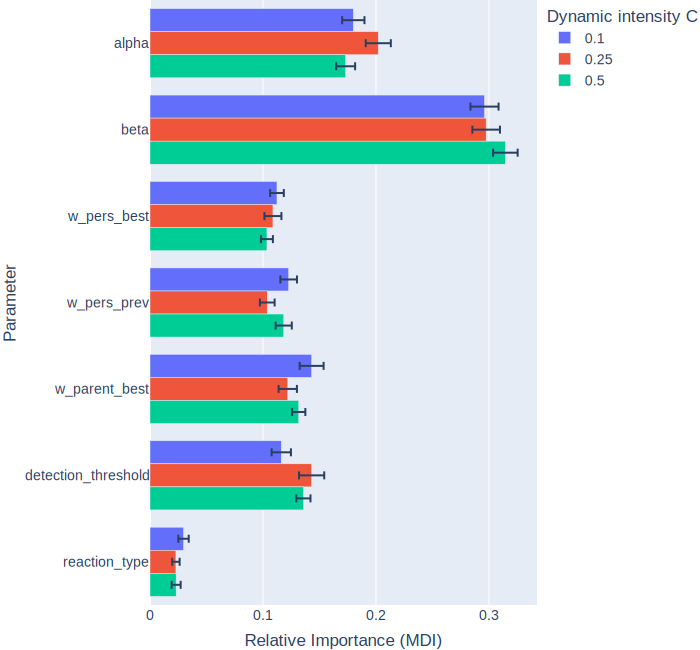
\includegraphics[width=1\textwidth]{results/part2/parameter_importance_bar_dynamic.svg}
	\caption[Bar chart of the parameter importance compared by dynamic intensity]{Bar plot of the parameter importance (\gls{mdi}) computed via the surrogate model over all 90 optimizer runs and compared by dynamic intensity $C$.}
	\label{fig:parameter_importance_bar_dynamic}
\end{figure}

The order of parameter importance does not change when the optimizer runs are grouped by their respective dynamic intensities $C$, as shown by the bar plot in \cref{fig:parameter_importance_bar_dynamic}. Here, the values are also discussed qualitatively for comparison, rather than giving the absolute \gls{mdi} values as before. Most of the differences in \gls{mdi} are within the margin of error, represented by the black whiskers at the right end of each bar. Only an increase in the importance of $\alpha$ and a slight decrease of $w_{\text{persprev}}$ and $w_{\text{parentbest}}$ are noticeable for medium dynamic intensities ($C=0.25$) compared to the other dynamics. Also, the detection threshold becomes slightly more important as the dynamic intensity increases, which could be expected from an increasingly changing problem environment, where improved change detection leads to better solutions. However, all these results are very close to the error margins of their groups and, as already mentioned, do not significantly change their relative importance compared to the values discussed in the previous table. 

\begin{figure}[h!]
	\centering
	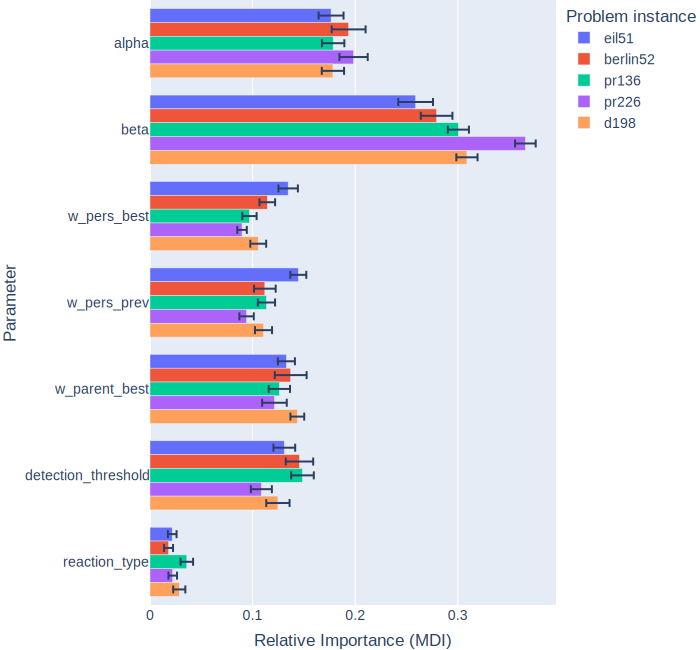
\includegraphics[width=1\textwidth]{results/part2/parameter_importance_bar_problem.svg}
	\caption[Bar plot of the parameter importance compared by problem instance]{Bar plot of the parameter importance (\gls{mdi}) computed via the surrogate model over all 90 optimizer runs and compared by problem instance.}
	\label{fig:parameter_importance_bar_problem}
\end{figure}

Similar findings can be made when grouping across problem instances, where the order parameter of parameter importance remains mostly the same. \Cref{fig:parameter_importance_bar_problem} shows only a few problem instances that change the importance for certain parameters. In particular, the highly clustered instance \texttt{pr226} has an importance of $\beta$ of over 0.35, more than any other instance, with a relatively low standard error. This instance also has $\alpha$ at about the same importance as the overall average, but the weights and detection threshold $\theta$ at even lower importance. In contrast, the very small and semi-regular instance \texttt{eil51} has the lowest importance out of all for $\beta$ and the highest \glspl{mdi} for the parameters $w_{\text{persbest}}$ and $w_{\text{persprev}}$, therefore suggesting an increasing relevance of the personal \gls{sce} populations for the solution creation process. In addition, instance \texttt{pr136} evaluated the reaction type $H$ as more important than any other problem instance. 

In summary, $\beta$ is undoubtedly the most important parameter for the surrogate model in every possible problem scenario, followed by $\alpha$ with about 10\% less relative importance. The three weights and the detection threshold $\theta$ are evaluated with varying importance depending on a certain dynamic intensity and problem instance, so that the importance gap to $\alpha$ is even smaller under some conditions. Finally, the reaction type appears to be the least important parameter, although this statement may be significantly invalidated by the cardinality bias of the \gls{mdi} method. 


\section{Part III - Evaluating the Parameter Sets}

The third part of the evaluation is based on the experimentation data of all ten \gls{tsp} instances, small and large, with all three dynamic intensities $C=\{0.1,0.25,0.5\}$, and each combination of instance and intensity was repeated $r_\text{exp} = 20$ using their specific optimal parameter set acquired by \gls{hpo}. As explained, all the parameters that have been acquired from smaller instances were used for the larger instance in the same structural group (see \cref{tab:best-parameters}). In addition to the \gls{hpo} parameter sets, a generally well-performing reference set based on the results of the original \gls{hsppbo} paper \cite{kupfer2021hierarchical} was used. In visualizations and comparisons, this is denoted as \enquote{Ref}. In contrast to the \gls{hpo} experiments, the parameter set for these reference experiments was the same for all combinations of instance and dynamics.

Furthermore, all graph and table data were computed by averaging the 20 repeated experimentation runs for each instance and dynamic intensity, and for aggregated or grouped data, they were also averaged across different dynamic intensities and/or \gls{tsp} instances. However, this is be mentioned where relevant. Since only \textit{TSPLIB} instances were used, the $RPD$, i.e. the relative difference to the optimal solution, was used to compare the solution quality, as in the first part of the results chapter. Also, as mentioned in \cref{chap:testing}, dynamic events start at iteration 2000 and occur at every next 100th iteration up until the last iteration at 2599. The time between each dynamic events is referred to as dynamic interval.

\subsection{Solution Quality}

After the first two result parts answered the two main research questions, we proceed to the fundamental, underlying question of whether or not these \gls{hpo} parameter sets produce satisfactory results at all. Therefore, the solution quality in the form of the previously used $RPD$ is shown over the course of the dynamic runtime, starting at iteration 1950, just before the first dynamic change is triggered at iteration 2000, and continuing until iteration 2399, omitting the last two dynamic events since they do not add any relevant data. 


\begin{figure}[h]
	\centering
	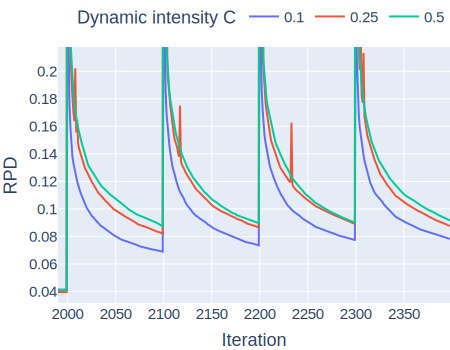
\includegraphics[width=0.7\textwidth]{results/part3/run_plot_cmp_dynamic_aggr_None_y_best_solution_1_to_30_HPO.svg}
	\caption[Line plots showing the $RPD$ over the dynamic iterations for all three dynamic intensities $C$]{Line plots showing the relative solution quality $RPD$ over the first 400 dynamic iterations (starting just before iteration 2000) for all three dynamic intensities $C$ averaged over all instances that used the \gls{hpo} parameter sets.}
	\label{fig:run_plot_cmp_dynamic_HPO}
\end{figure}

\Cref{fig:run_plot_cmp_dynamic_HPO} shows one of these run plots with different lines for each dynamic intensity $C$ and averaged over all \gls{tsp} instances. The first impressive aspect to note is that the solution quality just before the first dynamic event at iteration 2000 is exceptionally good for all dynamic intensities around $RPD=4\%$. Although the solution quality of the first 2000 iterations, representing the static \gls{tsp} problem, was only weighted with $1/7$, compared to the other six solution qualities taken just before the next dynamic event, the influence must have been sufficient for the \gls{hpo} process to produce good results here as well. 

Continuing to the first dynamic event at iteration 2000, there is an expected huge spike in solution quality for all three intensities, which continues along the y-axis up to $RPD=3$ and was truncated to increase the differentiation of the lines between the dynamic events. Interestingly, the medium dynamic intensity $C=0.25$ reached a higher value of $RPD=3$, while the solution quality for the higher dynamic $C=0.5$ did not spike as high to only $RPD=0.7$. This is mainly because the majority of parameter sets at $C=0.25$ used the full reset ($H_\text{full}$) as the change handling procedure, which resulted in significantly worse solution quality immediately after the change was detected, rather than the partial reset, where better performing solutions were still stored in the \gls{sce} tree. At iteration 2008 there is another spike, indicating a delayed execution of the change handling procedure, which can also be observed at different iterations in between each following dynamic interval. These spikes are also due to some specific instances that will be further analyzed at a later time. 

After these first 10 iterations following the dynamic event we observe a rapid increase in solution quality up to iteration 2099, with the parameter sets produced for the least dynamic problems $C=0.1$ clearly leading in $RPD$ value, achieving a solution only about 3\% worse than the static one. The $RPD$ values just before the next three dynamic events at 2200, 2300, and 2400 also show leading performance, although not as good as in this first interval. The solution qualities for the other two dynamic intensities also managed to improve to $RPD_{C=0.25}=0.8$ and $RPD_{C=0.5}=0.9$ just before the next dynamic event, which is also the case for the next three dynamic intervals. 

\begin{figure}[h]
	\centering
	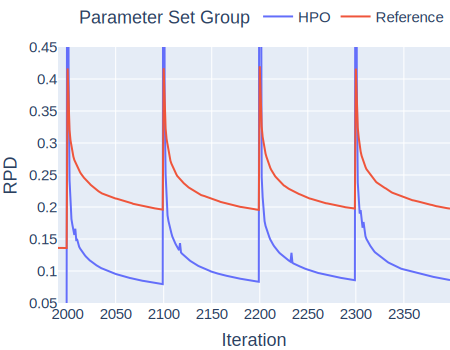
\includegraphics[width=0.65\textwidth]{results/part3/run_plot_cmp_folder_aggr_None_y_best_solution_1_to_30_HPO.svg}
	\caption[Line plots showing the relative solution quality $RPD$ over dynamic iterations for both parameter set groups averaged over dynamic intensities $C$ all \gls{tsp} instances.]{Line plots showing the relative solution quality $RPD$ over the first 400 dynamic iterations (starting just before iteration 2000) for both parameter set groups, \gls{hpo} and the reference set, averaged over all three dynamic intensities $C$ all ten \gls{tsp} instances.}
	\label{fig:run_plot_cmp_folder}
\end{figure}

To put these solution quality values into perspective, \cref{fig:run_plot_cmp_folder} shows the results for the reference parameter set in the same graph as the \gls{hpo} results, averaged over all dynamic intensities and \gls{tsp} instances. Although the reference set also produces acceptable results, the parameters obtained by \gls{hpo} clearly outperform them at every point in the dynamic runtime. Not only is the static solution more than three times better up to iteration 2000 than the reference parameter set ($RPD_\text{HPO} = 0.4$ vs. $RPD_\text{Ref}=0.14)$), the solutions obtained during each dynamic interval, just before the next dynamic event, are also significantly better with more than two times lower $RPD$ values of 0.08 compared to $RPD_\text{Ref}=0.2$. However, the reference parameter set appears to have no noticeable false detections of dynamic change in its dynamic intervals and also spikes to much lower $RPD$ values of just over 0.4.

When viewed separately for each dynamic intensity, as shown in \cref{fig:run_plot_cmp_folder_aggr_dynamic_HPO}, the impression does not change much. Just before each dynamic event, the reference parameter set consistently produced almost the same solution quality of $RPD_\text{Ref}=0.2$, while the \gls{hpo} parameter sets produced better results for lower dynamic intensities of $C=0.1$, as discussed above.

\begin{figure}[h]
	\centering
	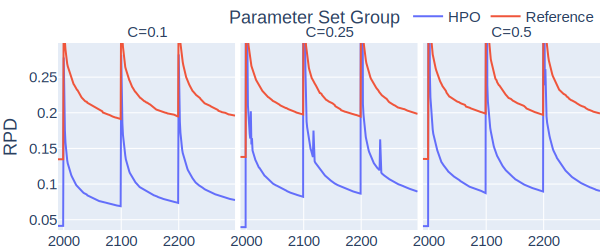
\includegraphics[width=0.85\textwidth]{results/part3/run_plot_cmp_folder_aggr_dynamic_y_best_solution_1_to_30_HPO.svg}
	\caption[Line plots showing the relative solution quality $RPD$ over dynamic iterations for both parameter set groups for each dynamic intensity$C$, averaged over \gls{tsp} instances]{Line plots showing the relative solution quality $RPD$ over the first 300 dynamic iterations (starting just before iteration 2000) for both parameter set groups, \gls{hpo} and the reference set, with a plot for each dynamic intensity$C$, averaged over all ten \gls{tsp} instances.}
	\label{fig:run_plot_cmp_folder_aggr_dynamic_HPO}
\end{figure}

\subsubsection{Problem Instance Generalization}
Next, we want to evaluate the problem classification and the proposed generalization of parameter sets obtained from smaller problem instances to larger instances of the same structural group. For this purpose, \cref{fig:run_plot_cmp_dynamic_aggr_problem_HPO} shows the run plots for each individual \gls{tsp} instance and each dynamic intensity $C$. The instance names are at the top of each plot and they are ordered in the same way as before in \cref{fig:cluster-groups}, so that the smaller instances are in the left column and the larger instances are in the right column, with each row corresponding to the predefined structural groups. Thus, each row of plots uses the same set of parameters when comparing dynamics.

\begin{figure}[p]
	\centering
	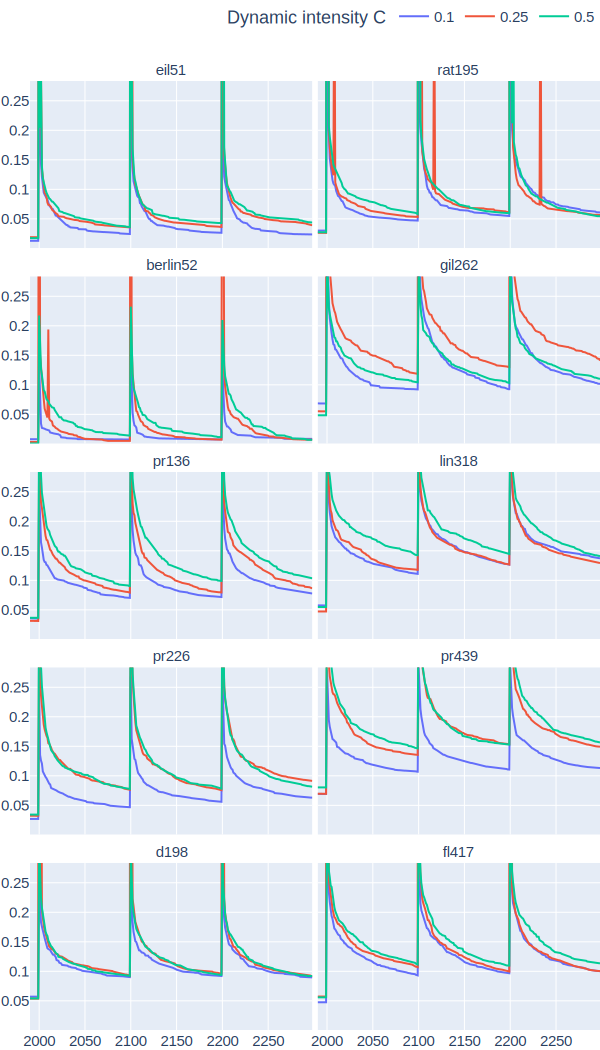
\includegraphics[width=0.725\textwidth]{results/part3/run_plot_cmp_dynamic_aggr_problem_y_best_solution_1_to_30_HPO.svg}
	\caption[Line plots showing the relative solution quality $RPD$ over dynamic iterations for all dynamic intensities $C$ and all \gls{tsp} instances for the \gls{hpo} experiments.]{Line plots showing the relative solution quality $RPD$ over the first 300 dynamic iterations (starting just before iteration 2000) for all three dynamic intensities $C$ and all ten \gls{tsp} instances for the \gls{hpo} experiments. The smaller instances are in the left column and the larger instances are in the right column. Each row corresponds to the predefined structural groups (see \cref{fig:cluster-groups}).}
	\label{fig:run_plot_cmp_dynamic_aggr_problem_HPO}
\end{figure}

The first row shows instances with random to nearly regular distribution. Although \texttt{rat195} has a dimension almost four times larger than \texttt{eil51}, the solution qualities for the static problem and the following dynamic intervals are very similar. With only a few percent worse $RPD$ values for \texttt{rat195} the overall performance just before the end of each dynamic interval is very satisfactory at around $RPD=0.05 \pm 0.01$. Furthermore, the static performance for \texttt{eil51} shows that it was almost perfectly solved for all three dynamic intensities at $RPD_{C=0.1}=0.01$ and $RPD_{C=0.25,0.5}=0.02$, which is even more interesting considering the use of very different parameters for each dynamic intensity. The larger pendant \texttt{rat195} also got very good static performance at around $RPD=0.025$, but has some significant cases of false dynamic detection, even resulting in spikes five iterations ($L_\text{pause} = 5$) after the dynamic event. 
Although both instances used the same parameter sets for $C=0.25$, the higher problem complexity resulted in an increase in \gls{sce} tree swaps many iterations after the dynamic event occurred, which then resulted in a large increases in $RPD$ because $H_\text{full}$ was used as the change handling procedure. 
The differences between the dynamic intensities are very small for both instances, which could be explained by the regular distribution of city nodes and therefore easier solution adaptation process after the problem change.

The second row contains \gls{tsp} instances with smaller, slightly clustered areas with an otherwise random structure. However, the two instances produced very different solution qualities. The \gls{hsppbo} algorithm almost always found the optimal solution in the static part for the smaller instance, \texttt{berlin52}, while the $RPD$ for \texttt{gil262} is only about 5\% just before the dynamic event at iteration 2000. Also, the parameter set used for the low dynamic intensity of $C=0.1$ produced a worse static solution quality than with the other two higher dynamic intensities. Looking at the parameter set in \cref{tab:best-parameters}, this could be explained by the use of the highest value for $\alpha$ across all parameter sets of  $\alpha = 3$, paired with the lowest $w_\text{parentbest}$ value of $w_\text{parentbest} = 0.196$. This could be due to the fact that \texttt{berlin52} has only one fifth of the city nodes of \texttt{gil262}, making it easier to find a good static solution, and the positive influence of these parameters on the dynamic performance. Another interesting observation for \texttt{gil262} is the worse dynamic performance of the parameter set for $C=0.25$ compared to $C=0.5$, although the results for \texttt{berlin52} do not show this behavior. Again, by looking at the parameters used, we can see that for $C=0.25$ a full reset of the \gls{sce} tree ($H_\text{full}$) was used with a very high dynamic detection threshold of $\theta=0.436$, thus making the algorithm less sensitive to dynamic changes in the problem instance. The instance \texttt{eil51} also used a similarly high $\theta = 0.46$ with $H_\text{full}$, but for a the high dynamic intensity of $C=0.5$, which produced better results because the dynamic detection threshold was likely reached more often.

The third row shows more consistent results when comparing the smaller instance, \texttt{pr136}, and the larger instance, \texttt{lin318}. These problems are artificially structured with certain patterns of medium clustered regions, with small distinct holes in the city distribution. The corresponding parameter sets use $\alpha = 2$, low $w_\text{persbest}$, and $H_\text{partial}$ for all three dynamic intensities. This resulted in good static performance just before the first dynamic event in iteration 1999, with $RPD$ values of just under 5\% for \texttt{pr136} and around 5\% for \texttt{lin318}.  The following first dynamic event shows very low spikes in $RPD$ with the highest value being 4\% for $C=0.5$. The increase in solution quality (and the decrease of the curve) seems to be less significant than for \texttt{berlin52} or the first row, and the $RPD$ values just before the next dynamic event do not come close to the static performance, especially for $C=0.5$ where the metaheuristic only obtained a solution of $RPD=0.1$ for \texttt{pr136} and $RPD=0.15$ for \texttt{lin318}, which is one of the worst results for any problem instance. The parameter sets for the two lower dynamic intensities can only marginally improve the $RPD$ values between dynamic intervals. The artificial pattern of city placement appears to make it more difficult to find good solutions after a dynamic change in a short amount of time.

The fourth row shows \gls{tsp} instances with few highly clustered areas, \texttt{pr226} and \texttt{pr439}, which produce a run curve very similar to the previous row. Interestingly, both structural groups share the same value range for the regularity index, which may explain their similar solution quality convergence behavior. They also show similarities in static performance, with \texttt{pr439} having a slightly worse solution quality, and the larger instance \texttt{pr439}, again showing one of the worst dynamic interval performances, only reaching $RPD_{C=0.25,0.5}=0.15$. However, the solution quality for the lowest dynamic $C=0.1$ is much lower for both small and large instances, with differences of up to 5\% in $RPD$, but only in dynamic situations. This suggests that the parameters seem to be highly tuned to perform well for small changes in the problem. Notable values in this set are very low $w_\text{persbest} = 0.112$ and $w_\text{persprev} = 0.051$, comparatively higher  $w_\text{parentbest} = 0.436$, and a low detection threshold of $\theta = 0.183$. Especially the last parameter could have a big impact on the good dynamic performance. However, other instances, such as \texttt{d198}, with a similar $\theta$ value at $C=0.1$ do not show the same good performance. This suggests that the structural characteristics of both problem instances may have had an influence.

The fifth and last row, with instances \texttt{d198} and \texttt{fl417}, represent a dispersed city placement, with highly clustered areas with few or no city nodes in between. The regularity index here is different from the previous two rows (groups). The convergence behavior between dynamic intervals is now more similar to the first row, with a rapid increase in solution quality in the first few iterations after the dynamic event, followed by a stagnation period up until the next dynamic event. Also, the difference between smaller and larger instance is the smallest out of all structural groups, with a gap of only 1-2\% for $C=0.5$. Interestingly, the static performance of the larger instance, \texttt{fl417}, is better than that of the smaller instance, \texttt{d198}, for $C=0.1$, which is also true for the first dynamic interval.

Compared to the same plots for the reference parameter set, shown in the \cref{chap:figures}, \cref{fig:run_plot_cmp_dynamic_aggr_problem_ref}, we can immediately confirm the conclusion from the aggregated plot above. The \gls{hpo} clearly outperforms the reference parameter set, with some instances showing significantly worse solution quality between dynamic events with $RPD$ values over 25\%. Also, the difference between dynamic intensities is not nearly as significant as for the \gls{hpo} parameters, suggesting that the tuning process specific to each dynamic intensity also seems to improve performance.

In summary, all ten \gls{tsp} instances show their own specific solution quality behavior and response to dynamic changes. Although a similar convergence behavior can be found within each structural group, which is also true for the plots for the reference parameter set, the data is not sufficient to suggest a clear relationship to the city placement characteristic. However, the generalization assumption can be confirmed to some extent, since all parameter sets for smaller instances also produced very good results for their larger counterparts. For a more profound evaluation of this aspect, a cross-validation of these parameter sets over different \gls{tsp} instances and dynamic intensities would have been necessary, but would have increased the number of experiments by a factor of 8.5. 

\subsection{Detection of Dynamic Changes}

A very important aspect of the \gls{hsppbo} metaheuristic is its ability to detect changes in the problem it solves and, in response, trigger a change handling procedure to respond optimally. Its performance in this regard depends solely on the dynamic detection threshold $\theta$ and its response mechanism on the $H$ mechanism, $H_\text{full}$ or $H_\text{partial}$. Without any prior knowledge of the way the \gls{hpo} method chooses these parameters, one would assume that, since the main goal is to obtain good solutions in dynamic environments, the correct detection of these changes is of high importance to the algorithm and thus to the \gls{hpo} method.
However, we have already discussed the minor importance of these two dynamic-relevant parameters in the previous results section (see \cref{chap:param-importance}).

Since the results in this respect deviate very strongly from this assumption, the general conclusion should already be anticipated.
With a few exceptions, related to specific combinations of instances and dynamics, and thus individual parameter sets, the correct detection of dynamic changes in the problem does not seem to have a particularly large effect on the solution quality of the \gls{hsppbo} algorithm when using \gls{hpo} parameter sets. More surprisingly, the reference parameter set outperforms the \gls{hpo} parameter sets in every discipline in terms of dynamic detection. This puts into perspective the exceptionally good solution quality performance of the \gls{hpo} parameter sets discussed before and raises the question of how relevant the correct detection of dynamic changes really is for good solutions to the \gls{dtsp}. To support these statements, the following graphs and tables provide performance metrics for many aspects of the dynamic detection behavior. 

First, the number of swaps, i.e., the changes within the \gls{sce} tree that eventually exceed the dynamic detection threshold $\theta$, is plotted over the first three dynamic intervals, similar to the solution quality plots from above. \Cref{fig:run_plot_cmp_dynamic_swaps} shows the results averaged over all ten \gls{tsp} instances, but separated by dynamic intensity $C$, represented by a line for each value. The left line plot shows the \gls{hpo} parameter sets, the right plot shows the reference parameter set. An additional dashed line was drawn for the reference parameter set, indicating the detection threshold $\theta = 0.25$, which results in $0.25 \cdot |A| = 3.25$ swaps required to trigger the change handling procedure. A similar line cannot be drawn for the \gls{hpo} plot because every \gls{tsp} instance uses its own $\theta$ value. A later plot, separated by problem instance, will show more details.

\begin{figure}[H]
	\centering
	\begin{subfigure}{0.515\textwidth}
		\centering
		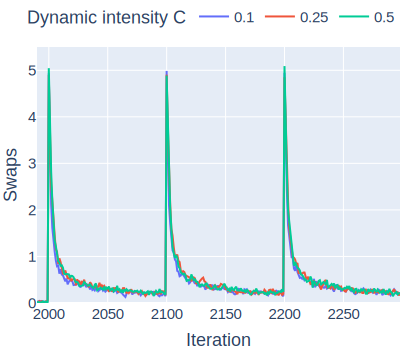
\includegraphics[width=\textwidth]{results/part3/run_plot_cmp_dynamic_aggr_None_y_swaps_1_to_30_HPO.svg}
		\caption{HPO}
		\label{fig:run_plot_cmp_dynamic_swaps_HPO}
	\end{subfigure}
	\begin{subfigure}{0.472\textwidth}
		\centering
		\raisebox{1.5pt}{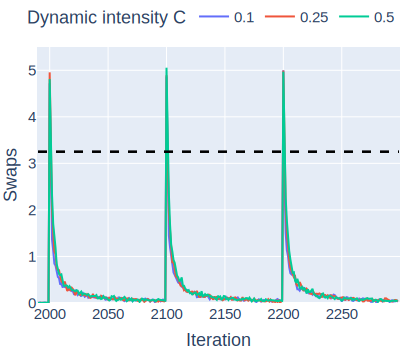
\includegraphics[width=\textwidth]{results/part3/run_plot_cmp_dynamic_aggr_None_y_swaps_1_to_30_Reference.svg}}
		\caption{Reference}
		\label{fig:run_plot_cmp_dynamic_swaps_Reference.svg}
	\end{subfigure}
	\caption[Line plots showing the swaps within the \gls{sce} tree over dynamic iterations for both parameter set groups showing all three dynamic intensities $C$, and averaged over \gls{tsp} instances.]{Line plots showing the relative solution quality swaps within the \gls{sce} tree over the first 300 dynamic iterations (starting just before iteration 2000) with a plot for each parameter set group, \gls{hpo} and the reference set, each showing all three dynamic intensities $C$, and averaged over all ten \gls{tsp} instances.}
	\label{fig:run_plot_cmp_dynamic_swaps}
\end{figure}

The first thing that is immediately noticeable is the similar number of swaps for both parameter groups, with an average of 5 swaps right at the dynamic event for all three dynamic intensities. This makes sense when considering the three levels of the \gls{sce} tree, where the first two levels are very likely to lose their high position when using the partial reset strategy $H_\text{partial}$, resulting in 4 swaps. However, the \gls{hsppbo} algorithm using the reference parameter set has its threshold at a reasonable level, which allows the dynamic response mechanism $H$ to be almost always correctly triggered immediately after the dynamic event. This partial reset allows the algorithm to find new, good solutions, which greatly reduces the number of swaps around 25 iterations after the dynamic event. Eventually, after the 50th iteration in each dynamic interval, the amount of swaps has been reduced to about $0.10 \pm 0.05$ for all the dynamic intensities. Compared to the \gls{hsppbo} results, the amount of swaps after this 50th iteration after each dynamic event is much higher at $0.30 \pm 0.1$, indicating that even long after the dynamic event has occurred, the algorithm is still finding better solutions than its direct parent node at about every third iteration. This suggests that either, the change handling procedure was not triggered, allowing old, possibly bad, solutions to influence the search for a longer time, or that the particular combination of parameters just performed enough exploratory behavior to still find increasingly better solutions at a later time. While the latter theory can be dismissed by looking at the almost identical convergence behavior of the solution quality comparison in \cref{fig:run_plot_cmp_folder}, the former theory is discussed later.

\begin{figure}[p]
	\centering
	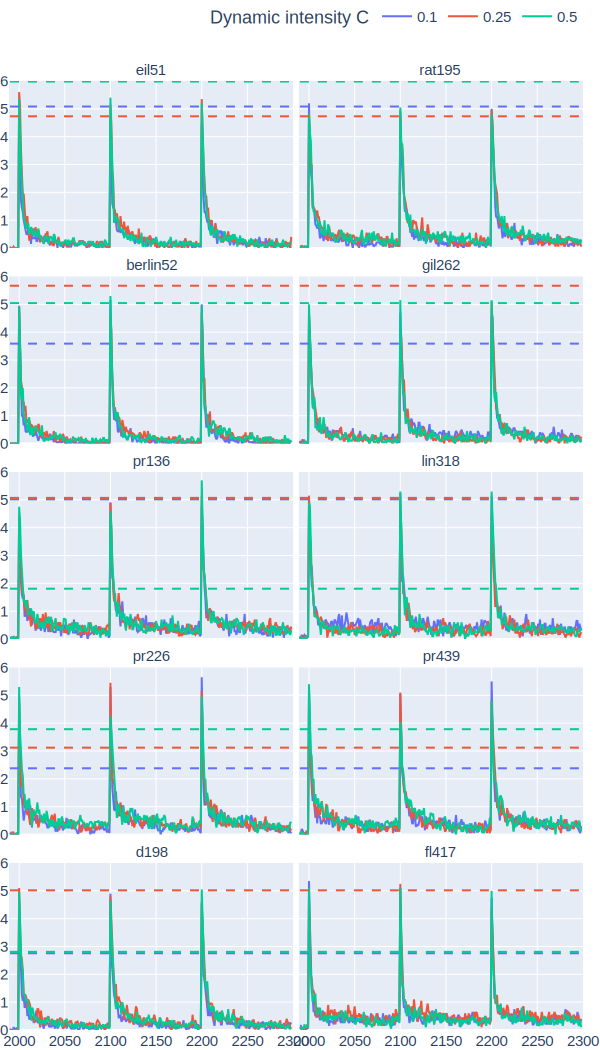
\includegraphics[width=0.725\textwidth]{results/part3/run_plot_cmp_dynamic_aggr_problem_y_swaps_1_to_30_HPO.svg}
	\caption[Line plots showing the swaps within the \gls{sce} tree over dynamic iterations for the \gls{hpo} parameter set showing all three dynamic intensities $C$ with a plot for each \gls{tsp} instance.]{Line plots showing the relative solution quality swaps within the \gls{sce} tree over the first 300 dynamic iterations (starting just before iteration 2000) for the \gls{hpo} parameter set showing all three dynamic intensities $C$ with a plot for each \gls{tsp} instance. The smaller instances are in the left column and the larger instances are in the right column. Each row corresponds to the predefined structural groups (see \cref{fig:cluster-groups}).}
		\label{fig:run_plot_cmp_dynamic_aggr_problem_swaps_HPO}
	\end{figure}

Continuing with \cref{fig:run_plot_cmp_dynamic_aggr_problem_swaps_HPO}, which shows the swaps over the first three dynamic intervals, this time also separated by problem instance, and only for the \gls{hpo} parameter sets, we can also draw dashed line representing the dynamic threshold that triggers $H$. As before, the instances are arranged according to their structural group and dimension. 
Looking at the first three rows, the thresholds for at least two of the dynamic intensities are very high at around 5 swaps, or even 6 in the case of \texttt{eil51} and \texttt{rat195}, using $\theta = 0.460$ for the highest dynamic intensity $C=0.5$. This threshold is almost never reached, and even the two thresholds for the lower dynamic intensities are only just passed in some cases. Another interesting aspect in the third and fifth row is that here the \gls{hpo} process chose the lowest detection threshold for the highest dynamic intensity $C=0.5$ at $\theta_\text{pr136} = 0.139$ and $\theta_\text{d198} =  0.216$, which is consistent with the results from the previous discussion in \cref{chap:robustness}. 
Furthermore, the amount of swaps after the 50th iteration in each dynamic interval remains high as seen before, with the smallest instances, \texttt{eil51} and \texttt{berlin52}, reaching a lower value level than other instances, such as \texttt{lin318} and \texttt{rat195}, which show a much higher average amount of swaps in the later stages of the dynamic interval. Thus, even though the same parameter sets were used in each row for each dynamic intensity, either the higher dimension or influences of the city placement characteristic had an impact on the number of swaps within each structural group.


In addition to the number of swaps, two performance metrics from machine learning classification, also used in information retrieval, were calculated on the data. As explained in \cref{chap:an-part3}, these metrics are precision and recall. The precision describes how many detected iterations (\gls{tp} + \gls{fp}) were actually \gls{tp}, and thus describing how relevant the detected iterations are. The recall describes how many possible correctly detectable iterations (positives) were actually detected by the \gls{hsppbo} algorithm (\gls{tp}). Both metrics span a range between 0 and 1, where 0 means that no correct detections (\gls{tp}) were found at all, and 1 means that either every dynamic event correctly triggered the change handling procedure, but allowing for \glspl{fp} (recall), or that all change handling procedures triggered were in response to a dynamic event, but allowing for dynamic events without any response (precision). The direct results of these metrics can also be found in \cref{tab:detection-stats-all-hpo} for the \gls{hpo} parameter set and \cref{tab:detection-stats-all-ref} for the reference parameter set, both inducing each combination of \gls{tsp} problem instance and dynamic intensity $C$.

In \gls{ml} visualization, these metrics are often presented in precision-recall curves for certain thresholds of classification confidence. A very good classifier will have a $PR$ curve close to $precision=1$ for varying recall values. A common baseline in these plots is a line parallel to the recall axis for the precision value representing the fraction of all positives to all negatives, with a good classifier staying above this line. In an example with equal amounts of positives and negatives, this line is drawn at $precision=0.5$, thus a random classifier could achieve this precision on average. When applied to this problem, the dynamic detection threshold of \gls{hsppbo} is not comparable to a classifier threshold, making it impractical to draw a curve or area plot from these precision and recall values. Instead, scatter plots were drawn with the baseline at $precision=30/570\approx0.053$. 

\begin{figure}[h]
	\centering
	\begin{subfigure}[b]{1\textwidth}
		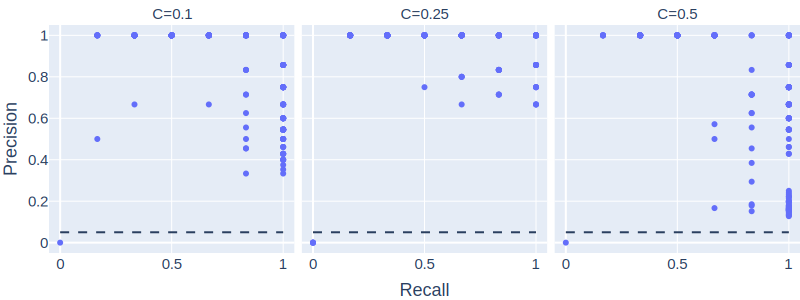
\includegraphics[width=1\textwidth]{results/part3/pr_curve_cmp_dynamic_grouped_False_HPO.svg}
		\caption{HPO}
		\label{fig:pr_curve_cmp_dynamic_HPO}
	\end{subfigure}
	\hfill
	\begin{subfigure}[b]{1\textwidth}
		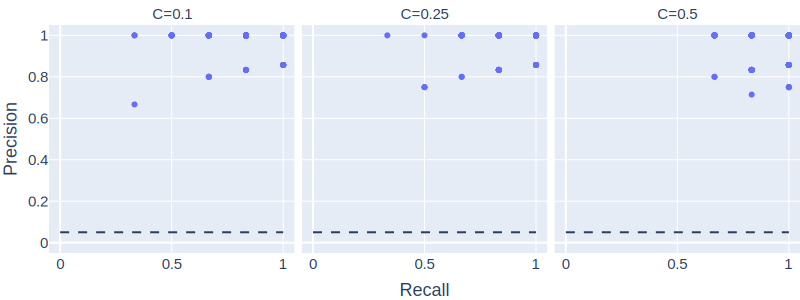
\includegraphics[width=1\textwidth]{results/part3/pr_curve_cmp_dynamic_grouped_False_Reference.svg}
		\caption{Reference}
		\label{fig:pr_curve_cmp_dynamic_Reference}
	\end{subfigure}
	\caption[Precision-Recall scatter plots separated by dynamic intensity $C$ for both parameter sets]{Precision-Recall scatter plots showing the values for recall on the x-axis and precision on the y-axis separated for each dynamic intensity $C$ (annotation at the top of the plots) for the \gls{hpo} (left) and the reference (right) parameter sets.}
	\label{fig:pr_curve_cmp_dynamic}
\end{figure}

\Cref{fig:pr_curve_cmp_dynamic} shows a $PR$ scatter plot for each dynamic intensity $C$, averaged over all \gls{tsp} instances, and compared for both the \gls{hpo} parameter set (\ref{fig:pr_curve_cmp_dynamic_HPO}) and the reference parameter set (\ref{fig:pr_curve_cmp_dynamic_Reference}). Again, the better dynamic detection performance of the reference set is clearly evident, with $PR$ points staying well above the precision baseline and mostly populating the upper right corner of the high precision and recall values, meaning that almost all dynamic events were found while avoiding \glsdesc{fp}. Interestingly, the performance on the least dynamic instances $C=0.1$ shows the worst $PR$ values at $recall = 0.33$ and $precision = 0.67$. This suggests that fewer dynamic events were detected in this case, which is to be expected since the static threshold of $\theta =0.25$ was reached less often. On the contrary, the highest dynamic intensity of $C=0.5$ showed the best $PR$ values.

Looking at the results for the \gls{hpo} parameter sets, the $PR$ values are more scattered, while generally performing worse, and sometimes coming close to the precision baseline. There even seemed to be multiple runs for all dynamic intensities where no dynamic events were detected ($PR = (0,0)$). 
The parameter sets for the medium dynamic intensity $C=0.25$ are able to obtain the best values for precision, when compared to the reference set. Although the highest dynamic intensity shows that many \gls{hsppbo} runs have detected all the dynamic events, reaching $recall =1$, the precision of these averaged runs was as low as $precision=0.13$. This indicates a very high amount of false detections (\gls{fp}) and thus false triggers of the change handling procedure. This is also partially true for the lowest dynamic intensity $C=0.1$, but the precision is slightly better, with the lowest value being $precision=0.33$, meaning that every third change handling procedure triggered was not a correct response to the dynamic event. This behavior could indicate that only in the case of medium dynamic intensity the \gls{hpo} considered a correct dynamic response as important enough for the goal of solution quality that it properly optimized for it. In contrast, especially with the choice of parameter values discussed before in mind (see \cref{fig:parameter_boxplot_dynamic}), the robust, high $\beta$ values for dynamic intensity $C=0.5$ and the robust, comparatively high $\alpha$ values for dynamic intensity $C=0.1$ suggest that for these dynamic environments, other parameters may be more important for good solution quality. This is also suggested in \cref{fig:parameter_importance_bar_dynamic}, although the higher importance of the detection threshold for $C=0.25$ lies in the error margin of the other two dynamic intensities.

\begin{figure}[h]
	\centering
	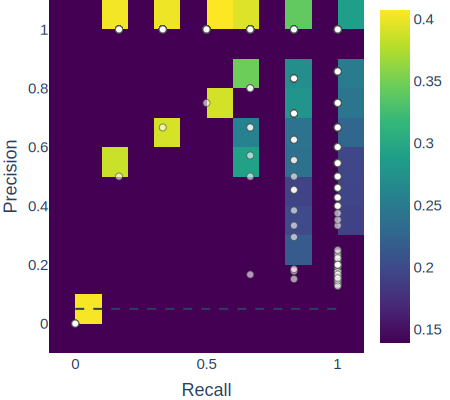
\includegraphics[width=0.55\textwidth]{results/part3/pr_curve_cmp_detection_threshold_grouped_True_HPO.svg}
	\caption[Precision-Recall heatmap showing the precision over the recall value with the z-axis displaying the detection threshold $\theta$ for the \gls{hpo} experiments]{Precision-Recall heatmap showing the precision over the recall value with the z-axis displaying the detection threshold $\theta$ as a color map for the \gls{hpo} experiments. The $\theta$ values for points in the same heatmap cell are averaged. In addition, the actual precision-recall points are overlayed to better seperate the darker areas.}
	\label{fig:pr_curve_cmp_detection_threshold}
\end{figure}

This relationship between high precision and recall values and the detection threshold seems to hold even more information about the dynamic detection capabilities of the \gls{hsppbo} metaheuristic. \Cref{fig:pr_curve_cmp_detection_threshold} shows the precision over the recall values, but with an underlying heatmap showing the detection threshold $\theta$ for the \gls{hpo} parameter set. Each heatmap cell represents the average $\theta$ value of all $PR$ points falling in that region, also called a bin. This is why the background appears to be covered by low $\theta$ values of 0.15, because this is the minimum value available for averaging and can be ignored if no point lies directly on that cell.
The worst performing runs with $PR = (0,0)$ used a very high detection threshold of $\theta \approx 0.4$, which requires 5 or more swaps in the \gls{sce} tree to trigger $H$. This value seems to be too high in almost all scenarios, because even the runs with $precision > 0.5$ using these high $\theta$ values only achieved suboptimal recall scores of $recall < 0.5$. This means that even though most of the $H$ triggers were correct responses to a dynamic event, more than half of the dynamic events went undetected. Looking at the near perfect upper right corner of $PR=(1,1)$, a dynamic detection value of $\theta = 0.29$ seems to be the best choice, which is very similar to the median seen in \cref{fig:parameter_boxplot}. While the recall remains high in the right section of the plot, the precision decreases with decreasing $\theta$ values.

Examining the $PR$ plot for each individual \gls{tsp} instance for the \gls{hpo} parameter set, shown in \cref{chap:figures} with \cref{fig:pr_curve_cmp_problem_HPO}, it appears that some instances achieved very good scores (e.g., the first two rows), while other instances had more problems with detecting dynamic events. However, this may very well be influenced by the parameters used rather than the problem instances themselves. Therefore, this visualization is not particularly significant and is only meant to further illustrate the effect of $\theta$ on the $PR$ scores.

\begin{figure}[h]
	\centering
	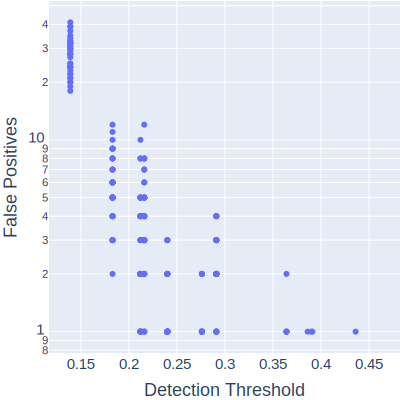
\includegraphics[width=0.5\textwidth]{results/part3/fp_theta_plot_HPO.svg}
	\caption[Scatter plot of all false dynamic detections by \gls{hsppbo} (\glsdesc{fp}) over the detection threshold $\theta$]{Scatter plot of all false dynamic detections by \gls{hsppbo} (\glsdesc{fp}) over the detection threshold $\theta$ for all 600 experimental runs using the \gls{hpo} parameter sets, using a logarithmic scale for the y-axis.}
	\label{fig:fp_theta_plot_HPO}
\end{figure}

Another interesting observation that proves that the dynamic detection works as expected is the relationship between \glsfirst{fp}, which are triggers of the change handling procedure that were not in correct response to a dynamic event, and the detection threshold $\theta$, shown in \cref{fig:fp_theta_plot_HPO}. A logarithmic y-axis was chosen because the \glspl{fp} increase exponentially with decreasing $\theta$. Therefore, we can clearly see an almost linear diagonal line from the upper left to the lower right of the scatter plot, suggesting that to greatly reduce false detections (to a fraction of $1/4$) from 40 to 10, we only need to slightly increase $\theta$ by 0.05 to $\theta = 0.19$,. However, any further reduction of \glspl{fp} can only be achieved by even higher increases in $\theta$ until a point is reached where we only have no false positives because we are not detecting anything at all.

\begin{table}[h]
	\setlength{\tabcolsep}{5pt}
	\centering
	\caption[The $F_1$ score averaged over all experimental runs for each combination of \gls{tsp} instance and dynamic intensity]{The $F_1$ score, i.e. the harmonic mean of the metrics precision and recall, and its standard error averaged over all $r_\text{exp} = 20$ experimental runs for each combination of \gls{tsp} instance (rows) and dynamic intensity $C$ (columns). Each element contains the values for the hyperparameter optimized parameters (\gls{hpo}, see \ref{tab:best-parameters}) and the reference parameter set (see \ref{tab:part3-gen-params}).}
	\label{tab:detection-stats-f1}
	\begin{adjustbox}{width=1\textwidth}
	\begin{tabular}{l  S[round-precision=2,table-format=1.2(2)] S[round-precision=2,table-format=1.2(2)]  S[round-precision=2,table-format=1.2(2)] S[round-precision=2,table-format=1.2(2)]  S[round-precision=2,table-format=1.2(2)] S[round-precision=2,table-format=1.2(2)]  S[round-precision=2,table-format=1.2(2)] S[round-precision=2,table-format=1.2(2)]}
		\hline
		 \gls{tsp} & \multicolumn{2}{c}{$C=0.10$} & \multicolumn{2}{c}{$C=0.25$} & \multicolumn{2}{c}{$C=0.50$} & \multicolumn{2}{c}{$\overline{C}$} \\ 
		 \cmidrule(lr){2-3} \cmidrule(lr){4-5}  \cmidrule(lr){6-7} \cmidrule(lr){8-9}
		~ & \text{HPO}  & \text{Ref.} & \text{HPO} & \text{Ref.} & \text{HPO} & \text{Ref.} & \text{HPO} & \text{Ref.}\\ \hline
		eil51 & 0.56(0.05) & 0.88(0.02) & 0.89(0.03) & 0.91(0.02) & 0.65(0.03) & 0.96(0.01) &0.70(0.03)& 0.92(0.01)\\
		rat195 & 0.63(0.04) & 0.89(0.02) & 0.86(0.02) & 0.94(0.01)  & 0.65(0.03) & 0.94(0.01) &0.71(0.02)&0.92(0.01)\\ \hline
		berlin52 & 0.92(0.01) &0.84(0.03)& 0.57(0.05) &0.95(0.02)& 0.59(0.05) & 0.93(0.02) &0.69(0.03)& 0.91(0.02)\\
		gil262 & 0.89(0.03) & 0.91(0.02) & 0.55(0.05) & 0.88(0.03)  & 0.66(0.04) &  0.96(0.01) &0.70(0.03)&0.92(0.01)\\ \hline
		pr136 & 0.61(0.04) & 0.89(0.02) & 0.56(0.05) & 0.92(0.02) & 0.27(0.01) & 0.96(0.02)  &0.48(0.03)&0.92(0.01)\\
		lin318 & 0.67(0.03) & 0.87(0.03) & 0.59(0.04) &  0.94(0.01) & 0.32(0.01) & 0.94(0.02)  &0.53(0.03)&0.92(0.01)\\ \hline
		pr226 & 0.66(0.01) & 0.91(0.02) & 0.88(0.02) & 0.91(0.02) & 0.84(0.03) & 0.94(0.02) &0.79(0.02)& 0.92(0.01)\\
		pr439 & 0.68(0.02) & 0.95(0.01) & 0.89(0.02) & 0.92(0.01) & 0.84(0.02) & 0.93(0.02) &0.80(0.02)& 0.93(0.01)\\ \hline
		d198 & 0.87(0.02) & 0.96(0.01) & 0.58(0.03) & 0.91(0.03) & 0.76(0.02) & 0.91(0.02) &0.73(0.02)&0.93(0.01) \\
		fl417 & 0.75(0.02) & 0.90(0.02) & 0.47(0.04) & 0.91(0.02) & 0.76(0.04) & 0.92(0.02) &0.66(0.03)& 0.91(0.01)\\ \hline
		$\overline{\text{\gls{tsp}}}$ & 0.72(0.01) & 0.90(0.01) & 0.68(0.02) & 0.92(0.01) & 0.63(0.02) & 0.94(0.00) &0.68(0.01)& 0.92(0.00)\\ \hline
	\end{tabular}
	\end{adjustbox}
\end{table}

Finally, all of the precision and recall values are combined into a harmonic mean, the so-called $F_1$ score, which is high, if both precision and recall are good, while a low $F_1$ score indicates poor performance in at least one of these aspects. It is particularly useful when the two metrics are of equal importance, as is the case here. The score is shown in \cref{tab:detection-stats-f1} for each combination of \gls{tsp} instance and dynamic detection threshold $C$, their respective means $\overline{\text{\gls{tsp}}}$ and $\overline{C}$, compared between the \gls{hpo} parameter sets and the reference set, with additional standard error from averaging. Each pair of rows separated by a line represents a structural group.

The data shows better dynamic detection by the reference parameter set than the \gls{hpo} sets in almost every direct comparison. Even more impressive, the reference value of $\theta = 0.25$ achieves values of $F_1 \geq 0.9$ in almost every combination of problem instance and dynamic intensity, with a total average over all values of $F_{1_\text{Ref}} = 0.92$. The total average of the \gls{hpo} parameter sets is 26\% lower at only $F_{1_\text{HPO}} = 0.68$. 
Only a few combinations of \gls{tsp} instance and dynamic intensity, and therefore specific parameter sets, were able to achieve satisfactory results. These exceptions are the first structural group with $C=0.25$ using a $\theta = 0.364$, the second structural group with $C=0.1$ using $\theta = 0.276$, the fourth group with $C=0.25$ using $\theta = 0.240$, and the fifth group with $C=0.1$ using $\theta = 0.212$. However, these exceptions are still worse than the scores in the same category obtained by the reference set, except for the second structural group, specifically \texttt{berlin52} with $C=0.1$, where $\theta = 0.276$, resulted in a $F_1$ score slightly better than that of the reference set.

In summary, the dynamic detection of the reference set using $\theta = 0.25$ almost always outperforms the parameter sets acquired by \gls{hpo}. This suggests that by using only the solution quality as a metric for the response to dynamic changes, the \gls{hpo} process, or at least the chosen \gls{gbrt} method, generally does not evaluate the correct dynamic detection as relevant to the search process, and thus, as expected in hindsight, values good solutions above all else. The superior solution quality has already been discussed before, leaving no doubt about the success of the \gls{hpo} process in that regard. However, it appears that unless the correct response to dynamic changes is explicitly made a requirement in the scoring function $f(\lambda)$, the process will not automatically include this goal in its search for well-performing parameters. The question then becomes whether this is even necessary if the solutions to the \gls{dtsp} are still remarkably good.

% !TeX root = main.tex
% !TeX spellcheck = en-US
% !TeX encoding = utf8


\chapter{Conclusion}
\label{chap:conclusion}

\glsresetall

In this thesis we successfully applied methods from \gls{hpo} to tune the parameters of the \gls{hsppbo} metaheuristic algorithm to solve the \gls{dtsp}. 
Not only did the parameters obtained by \gls{hpo} perform incredibly well in the dynamic phase of the \gls{dtsp}, but the static performance, just before the problem was changed, also showed admirable performance, especially when compared to a standard set of reference parameters for \gls{hsppbo}.

By planning and implementing all aspects necessary to answer the research questions, a new framework was derived, the \gls{xfopt}. Its main goal is to combine a variety of \gls{hpo} methods, such as \gls{rs}, \gls{bo}, and \gls{gbrt}, with the \gls{hsppbo} metaheuristic, all implemented in the \textit{Python} programming language. Moreover, it provides modularity and interfaces for each of the main modules, the problem, the optimizer, and the metaheuristic, allowing easy extensibility and ensuring potential future development based on the \gls{xfopt} framework. 
In light of the results discussed, it stands as a promising example of the potential that lies in the combination of \gls{hpo} and metaheuristics.

The effort to select appropriate test environments to efficiently perform all the necessary experiments and to analyze the huge amount of data obtained also proved to be worthwhile. The ten \gls{tsp} instances and the three dynamic intensities tested provided a well-rounded subset of problems. While the partitioning of the \gls{tsp} instances from the  \textit{TSPLIB} benchmark set into structural groups was ultimately not observed in the data analyzed, the goal of using disjoint subsets to reduce the number of experiments was still achieved, with all groups successfully generalizing their parameter sets to their larger counterparts. The parameter constraints postulated and used in the optimization process also proved to be correct, with the exception of $\beta$, which showed a clear ceiling effect. And the four \gls{hpo} methods tested presented a diverse selection, performing differently under given circumstances, each with its own advantages. The three parts of the experiments that were conducted all successfully served their purpose of answering the research questions, and during the data analysis no data was felt to be missing, due in large part to the automation of the process using a logging module that captured all the raw data outputs of the processes, and an analysis module that was able to calculate complex tabular results as well as visualize large amounts of data with different aggregations. However, due to the many repetitions of the \gls{hpo} procedure, and despite using two servers in parallel to compute the workload, the experiments took almost three months to complete.

The first research question, the choice of the ideal \gls{hpo} method for the \gls{hsppbo} metaheuristic, was answered in the first part of the results chapter. The arguments provided by convergence plots, \gls{auc} and minimum solution quality metrics, and statistical tests made it clear that \gls{gbrt} was the best choice for \gls{hsppbo}, since it almost always found the best solutions, while converging to them the fastest out of the the four methods compared. Furthermore, \gls{gp} and \gls{et} also showed very promising performance, with \gls{gp} in particular, excelling in \gls{tsp} instances of larger dimension.

The second question of what these best parameter sets look like was answered by the second part of the experiments. Here the results were more ambivalent. Although well-performing parameter sets were found for all specific combinations of problem instance and dynamic intensity, no clear recommendations for parameter values  could be made under most considerations. Except for $\alpha$ and $\beta$, which also seemed to be the most important parameters for the trained \gls{gbrt} surrogate model, and the favored use of the partial reset as the change handling procedure, only improved parameter value ranges were given for the remaining parameters, the three weights, and the detection threshold. In addition, no significant zero order correlation was found between these parameters. 

In the final results chapter, all of these findings were combined - using the best \gls{hpo} method to generate the best parameter values for each combination of problem instance and dynamic intensity - and compared to a well-performing reference parameter set. In terms of solution quality, the \gls{hpo} parameters showed excellent results across all problem descriptions and throughout the runtime. However, it was found that this good solution quality was not due to the correct detection of dynamic changes, but was achieved despite their absence. The reference parameter set outperformed the \gls{hpo} parameters in every discipline regarding dynamic detection, which was explained by either too low or too high choices for the detection threshold $\theta$.

In summary, \gls{hpo} has great potential for tuning the parameters of \gls{hsppbo} and possibly metaheuristics in general. Different optimization methods have different effects on the resulting parameter values and on the problems on which they are obtained on. No single set of parameter values can be recommended to solve all \gls{dtsp} problem descriptions, be they instance or dynamic. However, through the efficient application of \gls{hpo} methods, such a general-purpose parameter set can easily be replaced by a parameter set specifically tuned for a given problem. In the case of \gls{hsppbo}, it is debatable whether good performance on the \gls{dtsp} should be achieved by constructing highly greedy-influenced \glspl{sce}, or by correct detection of dynamic events, and also which parameters influence the solution quality the most.

\section{Future Work}

On many occasions throughout the thesis, thoughts were given about possible future work and research. 
To further improve the solution quality, new parameter value ranges and fixed value recommendations were presented (see \cref{chap:param-recommend}), which are an ideal starting point for new experiments with any kind of \gls{hpo} method. In this context, the good performance of the \gls{gp} method for \gls{tsp} instances of larger dimension ($>150$) could be further analyzed, especially in comparison with \gls{gbrt}. Also, a cross-validation of \gls{hpo} parameter sets obtained for different problem descriptions could be done to investigate, how specific they are tied to their original problem and how well they can be generalized. 
Since the optimization results focus on the parameters that lead to the best solution quality, the experiments were also prepared with this goal in mind. This raises two interesting topics that could not be answered with the available data. First, the tuning of the \gls{hpo} process itself could significantly reduce the time needed for a parameter set. Thus, experiments should be conducted on the minimum number of objective calls required, different initial sampling methods, and other ways to make \gls{hpo} more suitable for online use. The second possibility for future work to optimize the \gls{hpo} process is the evaluation of different solution scoring functions $f(\mathbf{\lambda})$, which could strongly influence what kind of \enquote{good} solutions are found. 
This is also where the lack of dynamic performance can be addressed by including the correct detection of dynamic events in the evaluation function that gives feedback to \gls{hpo}. Implementing the precision and recall metrics described above in the function would be one way to do this.

Finally, the data sets obtained in this thesis offer an intriguing possibility of replacing \gls{hpo} by using \gls{ml} models for parameter inference in a metaheuristic algorithm. The experiments resulted in numerous parameter sets that produced near-optimal solutions, along with detailed meta-information about each run, problem instance, city placement properties, and dynamic aspects. While the problem description was found to have a significant influence on the optimal parameters, direct correlations between parameter values and problems were not observed, suggesting higher-order relationships. Therefore, a \gls{ml} model capable of capturing these complex relationships is proposed. The training set would include experimental data, particularly from the second part, with input features represented by meta-information about the problem environment ($R$, $\lambda_1$, or $CQV$). The dynamics could be described by specific measures ($C$ or $T_d$) or generalized categories. The output or label would be the chosen parameters for a given problem description. Two possible approaches for training the model can be used: supervised learning using the best parameter sets only, or reinforcement learning that also incorporates poorly performing sets. Supervised learning, while limited by available \gls{hpo} data, offers easier preprocessing and implementation, potentially achieving satisfactory accuracy with simple methods. On the other hand, reinforcement learning requires more data and training time but may lead to better accuracy and generalization. Regardless of the chosen ML method, the trained model would enable inferring optimal parameter values for any \gls{tsp} problem description.

However good this \glsdesc{ml} option might be, training such a model would be a challenge in and of itself, not to mention the training data that would be required. In contrast, the possibility of \gls{hpo} for metaheuristics, discussed here and supported by evidence, should be the primary focus of future work.

\chapter*{Abstract}

This master's thesis in computer science explores the application of \glsfirst{hpo} methods to tune the parameters of the \glsfirst{hsppbo} metaheuristic algorithm for solving the \glsfirst{dtsp}. The work combines various \gls{hpo} methods with the \gls{hsppbo} metaheuristic. The experiments were conducted using ten \gls{tsp} instances and three dynamic intensities to realize the \gls{dtsp}. The first research question about the ideal \gls{hpo} method was answered by comparing the performance of four different methods and found \gls{gbrt} to be the leading method. The second question investigated the best parameter sets for each combination of the problem instance and dynamic intensity, yielding interesting results about the robustness and importance of certain parameters, as well as the insight that no single parameter set is the best choice for all problem descriptions. The third part of the results compared the performance of the \gls{hpo} parameters to a reference parameter set, showing that the \gls{hpo} parameters performed excellently in the \gls{dtsp}, but the reference set outperformed them in dynamic detection. Overall, the work demonstrates the potential of \gls{hpo} in tuning metaheuristic parameters.

\small	
\textbf{\textit{Keywords---}}
 \glsfirst{hpo}, Metaheuristics, Parameter Tuning, \glsfirst{dtsp},  \glsfirst{hsppbo}, Python, \glsfirst{rs}, \glsfirst{bo}, \glsfirst{gp}, \glsfirst{et}, \glsfirst{gbrt}

\printbibliography

%All links were last followed on March 1, 2023.

% Abkürzungsverzeichnis
\printnoidxglossaries

\listoffigures
\listoftables

%Wird nur bei Verwendung von der lstlisting-Umgebung mit dem "caption"-Parameter benoetigt
%\lstlistoflistings
%ansonsten:
\listof{Listing}{List of Listings}

%mittels \newfloat wurde die Algorithmus-Gleitumgebung definiert.
%Mit folgendem Befehl werden alle floats dieses Typs ausgegeben
%\listof{Algorithmus}{List of Algorithms}
\listofalgorithms %Ist nur für Algorithmen, die mittels \begin{algorithm} umschlossen werden, nötig


\appendix

\chapter{Additional Figures}
\label{chap:figures}

\begin{figure}[h]
	\centering
	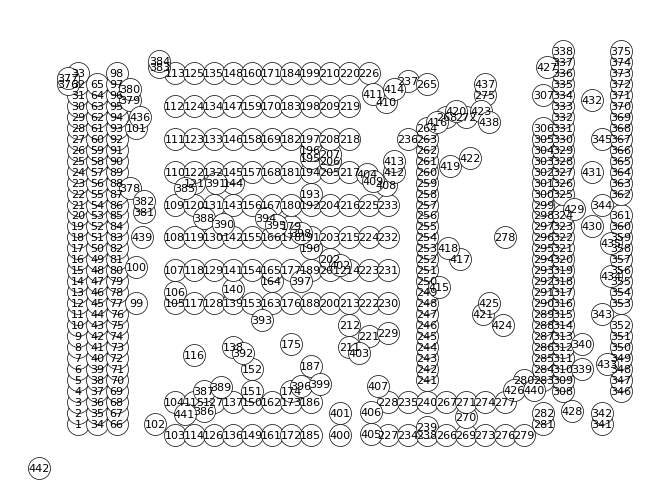
\includegraphics[width=0.6\textwidth]{pcb442.png}
	\caption{Visualization of the \gls{tsp} instance \textit{pcb442}.}
	\label{fig:pcb442}
\end{figure}
\begin{figure}[h]
	\centering
	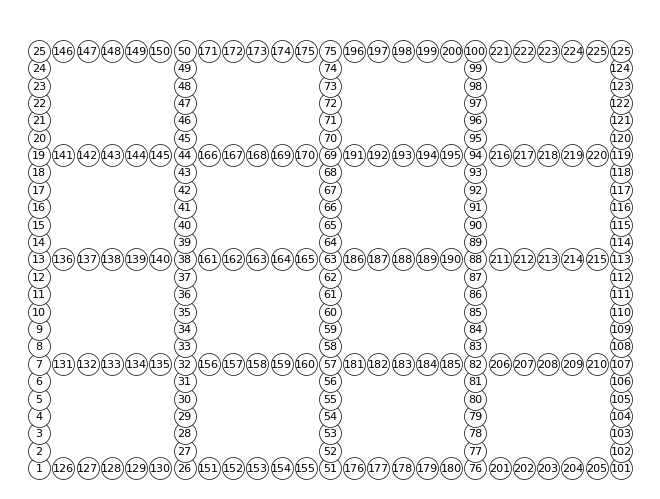
\includegraphics[width=0.6\textwidth]{ts225.png}
	\caption{Visualization of the \gls{tsp} instance \textit{ts225}.}
	\label{fig:ts225}
\end{figure}

\begin{figure}[h]
	\centering
	\includegraphics[width=\textwidth]{results/part2/param_scatter_matrix_None_with_H.svg}
	\caption[Scatter matrix plot of all \gls{hsppbo} parameters]{Scatter matrix plot of all \gls{hsppbo} parameters (except $H$) over all 90 optimizer runs with reaction type.}
	\label{fig:parameter_scatter_matrix_added}
\end{figure}
\begin{figure}[h]
	\centering
	\includegraphics[width=0.6\textwidth]{results/part2/alpha_weight_semilog_plot.svg}
	\caption[Scatter plot of all $\alpha$-values over the sum of the three weights]{Scatter plot of all $\alpha$-values over the sum of the three weights on a logarithmic scale over all 90 optimizer runs.}
	\label{fig:alpha_weight_semilog_plot}
\end{figure}

\begin{figure}[h!]
	\centering
	\includegraphics[width=0.725\textwidth]{results/part3/run_plot_cmp_dynamic_aggr_problem_y_best_solution_1_to_30_Reference.svg}
	\caption[Line plots showing the relative solution quality $RPD$ over dynamic iterations for all dynamic intensities $C$ and all \gls{tsp} instances for the \gls{hpo} experiments.]{Line plots showing the relative solution quality $RPD$ over the first 300 dynamic iterations (starting just before iteration 2000) for all three dynamic intensities $C$ and all ten \gls{tsp} instances for the reference experiments. The smaller instances are in the left column and the larger instances are in the right column. Each row corresponds to the predefined structural groups (see \cref{fig:cluster-groups}).}
	\label{fig:run_plot_cmp_dynamic_aggr_problem_ref}
\end{figure}

\begin{figure}[h]
	\centering
	\includegraphics[width=0.5\textwidth]{results/part3/pr_curve_cmp_problem_grouped_False_HPO.svg}
	\caption[Precision-Recall scatter plots separated by \gls{tsp} instance for the \gls{hpo} parameter sets]{Precision-Recall scatter plots showing the values for recall on the x-axis and precision on the y-axis separated for each of the 10 \gls{tsp} instances (name atop the plots) for the \gls{hpo} parameter sets. The smaller instances are in the left column and the larger instances are in the right column. Each row corresponds to the predefined structural groups (see \cref{fig:cluster-groups}).}
	\label{fig:pr_curve_cmp_problem_HPO}
\end{figure}


\chapter{Additional Tables}
\label{chap:tables}

\begin{table}[h]
	\centering
	\caption{Statistical values from the parameter box plots in \cref{fig:parameter_boxplot}.}
	\label{tab:parameter_boxplot}
	\begin{tabular}{c | S[round-precision = 0]S[round-precision = 0]SSSS}
		\hline
		Quartile & $\alpha$ & $\beta$ & $w_{\text{persbest}}$ & $w_{\text{persprev}}$& $w_{\text{parentbest}}$ & $\theta$ \\ \hline
		$Q_0$ & 1.0 & 4.0 & 0.0017540098159148 & 0.0013058587343205 & 0.0243455716583838 & 0.1000586776952464 \\ 
		$Q_1$ & 1.0 & 8.0 & 0.10820985322804134 & 0.0982650186608865 & 0.39772659356367485 & 0.2031240397284998 \\ 
		$Q_2$ & 2.0 & 9.0 & 0.3668190220597013 & 0.35038694215331323 & 0.666735344822367 & 0.30754351299901894 \\ 
		$Q_3$ & 2.0 & 10.0 & 0.8207074858781983 & 0.6620793002334411 & 0.8737596272590923 & 0.42612816877235665 \\ 
		$Q_4$ & 5.0 & 10.0 & 0.9838055744003416 & 0.9823508170176072 & 0.989433046328721 & 0.4965211978807402 \\ \hline
	\end{tabular}
\end{table}

\begin{table}[!ht]
	\centering
	\caption[Statistical values from the parameter box plots in \cref{fig:parameter_boxplot_dynamic}]{Statistical values from the parameter box plots in \cref{fig:parameter_boxplot_dynamic}, grouped over dynamic intensity $C$.}
	\label{tab:parameter_boxplot_dynamic}
	\begin{tabular}{cc | S[round-precision = 0]S[round-precision = 0]SSSS}
		\hline
		$C$ & Quartile & $\alpha$ & $\beta$ & $w_{\text{persbest}}$ & $w_{\text{persprev}}$& $w_{\text{parentbest}}$ & $\theta$ \\ \hline
		\multirow{5}{*}{0.1} & $Q_0$ & 1.0 & 4.0 & 0.0017540098159148 & 0.0084471729216077 & 0.1814385051209235 & 0.1059947155622872 \\ 
		 & $Q_1$ & 2.0 & 7.25 & 0.1005677137258057 & 0.10290369037238857 & 0.42220410885117776 & 0.26597396370492493 \\ 
		 & $Q_2$ & 2.0 & 9.5 & 0.2524117367709231 & 0.4359440557769896 & 0.6712685135069866 & 0.3488017264644777 \\ 
		 & $Q_3$ & 2.0 & 10.0 & 0.6934555352303847 & 0.6862216612986716 & 0.8139487205714664 & 0.44606148020261915 \\ 
		 & $Q_4$ & 5.0 & 10.0 & 0.9803318043883088 & 0.9823508170176072 & 0.9878070384965864 & 0.4927694284042387 \\ \hline
		 
		\multirow{5}{*}{0.25} & $Q_0$ & 1.0 & 7.0 & 0.0024046982167409 & 0.0013058587343205 & 0.129591588157158 & 0.100402723603361 \\ 
		& $Q_1$ & 1.25 & 8.25 & 0.0756733819115922 & 0.06347229865149373 & 0.2997311907279866 & 0.23890461234152374 \\ 
		& $Q_2$ & 2.0 & 9.0 & 0.2808847629983642 & 0.23037010247063974 & 0.5495721396059188 & 0.3486441528035795 \\ 
		& $Q_3$ & 2.0 & 10.0 & 0.8197824391868092 & 0.5122486803126786 & 0.9271467833023219 & 0.4174973602208792 \\ 
		& $Q_4$ & 3.0 & 10.0 & 0.9838055744003416 & 0.9749494820560152 & 0.9860696229889464 & 0.4965211978807402 \\ \hline
		\multirow{5}{*}{0.5} & $Q_0$ & 1.0 & 6.0 & 0.0085451982069353 & 0.0034068150552626 & 0.0243455716583838 & 0.1000586776952464 \\ 
		& $Q_1$ & 1.0 & 9.0 & 0.2166259934284717 & 0.1313765063425955 & 0.4881966058121041 & 0.17155855114994417 \\ 
		& $Q_2$ & 1.0 & 9.5 & 0.4424909342602664 & 0.3817891397291451 & 0.6673058638088523 & 0.26602176618163476 \\ 
		& $Q_3$ & 2.0 & 10.0 & 0.8883556777974986 & 0.7080535723858377 & 0.9678397769501375 & 0.3297181067512992 \\ 
		& $Q_4$ & 3.0 & 10.0 & 0.9819332671626134 & 0.9669078157348256 & 0.989433046328721 & 0.4906838085326337 \\ \hline
	\end{tabular}
\end{table}

\begin{table}[h]
	\centering
	\caption[Statistical values from the parameter box plots in \cref{fig:parameter_boxplot_problem}]{Statistical values from the parameter box plots in \cref{fig:parameter_boxplot_problem}, grouped over \gls{tsp} problem instance.}
	\label{tab:parameter_boxplot_problem}
	\begin{tabular}{cc | S[round-precision = 0]S[round-precision = 0]SSSS}
		\hline
		TSP & Quartile & $\alpha$ & $\beta$ & $w_{\text{persbest}}$ & $w_{\text{persprev}}$& $w_{\text{parentbest}}$ & $\theta$ \\ \hline
		\multirow{5}{*}{\texttt{eil51}} & $Q_0$ & 1.0 & 5.0 & 0.0085451982069353 & 0.0013058587343205 & 0.1699358970472349 & 0.1005034943221183 \\ 
		& $Q_1$ & 1.0 & 7.0 & 0.10135340878954588 & 0.2923295422518103 & 0.2808141602427695 & 0.19402792053206736 \\ 
		& $Q_2$ & 2.0 & 8.5 & 0.19506233867669576 & 0.5035011424279894 & 0.5970520438033792 & 0.3329379646556321 \\ 
		& $Q_3$ & 2.0 & 9.75 & 0.9610105456991581 & 0.7922314503372154 & 0.8831147115696516 & 0.40440632614592065 \\ 
		& $Q_4$ & 5.0 & 10.0 & 0.9838055744003416 & 0.9669078157348256 & 0.989433046328721 & 0.4673532156 559051 \\ \hline
		\multirow{5}{*}{\texttt{berlin52}} & $Q_0$ & 1.0 & 4.0 & 0.0448916769013341 & 0.0034068150552626 & 0.1957091892595615 & 0.100402723603361 \\ 
		 & $Q_1$ & 1.0 & 9.0 & 0.16290056250647555 & 0.0862693618778358 & 0.41220875467143864 & 0.2996433070789324 \\ 
		 & $Q_2$ & 1.5 & 9.0 & 0.3541885505731906 & 0.18758903878815208 & 0.774596480040849 & 0.40416254244584804 \\ 
		 & $Q_3$ & 2.0 & 10.0 & 0.7322042445175949 & 0.5789464829517041 & 0.8673312356740198 & 0.44390531279820805 \\ 
		 & $Q_4$ & 3.0 & 10.0 & 0.9722697857083962 & 0.962226698303581 & 0.9860696229889464 & 0.4965211978807402 \\ \hline
		\multirow{5}{*}{\texttt{pr136}} & $Q_0$ & 1.0 & 7.0 & 0.0024046982167409 & 0.0084471729216077 & 0.1744182996441411 & 0.1000586776952464 \\ 
		 & $Q_1$ & 2.0 & 8.0 & 0.084477671542753 & 0.0994553280739396 & 0.3386291701658647 & 0.19252755982109943 \\ 
		 & $Q_2$ & 2.0 & 9.0 & 0.3489873770996918 & 0.275681327119771 & 0.5027759615499374 & 0.29841749974430076 \\ 
		 & $Q_3$ & 2.0 & 10.0 & 0.6769431161929184 & 0.376132302143883 & 0.7809241481590734 & 0.4020634566190981 \\ 
		 & $Q_4$ & 3.0 & 10.0 & 0.9792102227882592 & 0.9823508170176072 & 0.98570021775642 & 0.4677200918763524 \\ \hline
		\multirow{5}{*}{\texttt{pr226}} & $Q_0$ & 1.0 & 8.0 & 0.0031534275907055 & 0.0136879948159208 & 0.0243455716583838 & 0.1059947155622872 \\ 
		 & $Q_1$ & 1.0 & 9.0 & 0.07396816934154625 & 0.1556039242180109 & 0.37314806391257294 & 0.1582724734544096 \\ 
		 & $Q_2$ & 2.0 & 10.0 & 0.2169825629531053 & 0.4424258653177224 & 0.7128991594867584 & 0.222064161198446 \\ 
		 & $Q_3$ & 2.0 & 10.0 & 0.7592318401240349 & 0.6209019085030367 & 0.951987131880033 & 0.29033282542957684 \\ 
		 & $Q_4$ & 3.0 & 10.0 & 0.9819332671626134 & 0.9116711549940856 & 0.9878070384965864 & 0.4756053754634357 \\ \hline
		 \multirow{5}{*}{\texttt{d198}} & $Q_0$ & 1.0 & 7.0 & 0.0017540098159148 & 0.0165137768209524 & 0.4174754411299966 & 0.1369961001761 \\ 
		 & $Q_1$ & 2.0 & 9.25 & 0.24497733011419962 & 0.06347229865149373 & 0.6057024502764778 & 0.22423375764498227 \\ 
		 & $Q_2$ & 2.0 & 10.0 & 0.6064500519993586 & 0.1024485693462489 & 0.6858898056605821 & 0.36179501748617793 \\ 
		 & $Q_3$& 3.0 & 10.0 & 0.804443382519819 & 0.7081029725955907 & 0.882319724646485 & 0.45718645820450626 \\ 
		 & $Q_4$ & 4.0 & 10.0 & 0.9352368688062224 & 0.9749494820560152 & 0.9846124119884476 & 0.4927694284042387 \\ 
	\end{tabular}
\end{table}

\begin{table}
	\centering
	\caption[Information retrieval performance metrics averaged over all experimental runs for each combination of \gls{tsp} instance and dynamic intensity for the \gls{hpo} parameter sets]{Information retrieval or classification performance metrics averaged over all $r_\text{exp} = 20$ experimental runs for each combination of \gls{tsp} instance (rows) and dynamic intensity $C$ (columns) for the \gls{hpo} parameter sets  (see \ref{tab:best-parameters}).}
	\label{tab:detection-stats-all-hpo}
	\begin{tabular}{l S[round-precision=2,table-format=1.2] | S[round-precision=0,table-format=1.0] S[round-precision=0,table-format=1.0]  S[round-precision=3,table-format=1.3] S[round-precision=2,table-format=1.2] S[round-precision=2,table-format=1.2] S[round-precision=2,table-format=1.2(2)]}
		\hline
		\gls{tsp}& \text{$C$} &{\thead{True\\Positives}} & {\thead{False\\Positives}} & {\thead{False\\Positive Rate}} & \text{Recall} & \text{Precision} & \text{$F_1$} \\
		\hline
		\multirow[c]{3}{*}{eil51} & 0.100000 & 2.500000 & 0.000000 & 0.000000 & 0.416667 & 0.950000 & 0.56(0.05) \\
		& 0.250000 & 4.900000 & 0.000000 & 0.000000 & 0.816667 & 1.000000 & 0.89(0.03) \\
		& 0.500000 & 3.000000 & 0.000000 & 0.000000 & 0.500000 & 1.000000 & 0.65(0.03) \\ \hline
		\multirow[c]{3}{*}{rat195} & 0.100000 & 2.900000 & 0.050000 & 0.000088 & 0.483333 & 0.983333 & 0.63(0.04) \\
		& 0.250000 & 4.800000 & 0.300000 & 0.000526 & 0.800000 & 0.951905 & 0.86(0.02) \\
		& 0.500000 & 3.000000 & 0.000000 & 0.000000 & 0.500000 & 1.000000 & 0.65(0.03) \\ \hline
		\multirow[c]{3}{*}{berlin52} & 0.100000 & 5.500000 & 0.450000 & 0.000789 & 0.916667 & 0.941071 & 0.92(0.01) \\
		& 0.250000 & 2.600000 & 0.050000 & 0.000088 & 0.433333 & 0.940000 & 0.57(0.05) \\
		& 0.500000 & 2.650000 & 0.000000 & 0.000000 & 0.441667 & 0.950000 & 0.59(0.05) \\ \hline
		\multirow[c]{3}{*}{gil262} & 0.100000 & 5.350000 & 0.500000 & 0.000877 & 0.891667 & 0.923810 & 0.89(0.03) \\
		& 0.250000 & 2.400000 & 0.000000 & 0.000000 & 0.400000 & 0.950000 & 0.55(0.05) \\
		& 0.500000 & 3.150000 & 0.000000 & 0.000000 & 0.525000 & 1.000000 & 0.66(0.04) \\ \hline
		\multirow[c]{3}{*}{pr136} & 0.100000 & 2.800000 & 0.050000 & 0.000088 & 0.466667 & 0.975000 & 0.61(0.04) \\
		& 0.250000 & 2.550000 & 0.050000 & 0.000088 & 0.425000 & 0.937500 & 0.56(0.05) \\
		& 0.500000 & 5.900000 & 32.100000 & 0.056316 & 0.983333 & 0.156880 & 0.27(0.01) \\ \hline
		\multirow[c]{3}{*}{lin318} & 0.100000 & 3.100000 & 0.000000 & 0.000000 & 0.516667 & 1.000000 & 0.67(0.03) \\
		& 0.250000 & 2.650000 & 0.000000 & 0.000000 & 0.441667 & 1.000000 & 0.59(0.04) \\
		& 0.500000 & 5.850000 & 24.550000 & 0.043070 & 0.975000 & 0.195598 & 0.32(0.01) \\
		\multirow[c]{3}{*}{pr226} & 0.100000 & 5.950000 & 6.300000 & 0.011053 & 0.991667 & 0.493272 & 0.66(0.01) \\
		& 0.250000 & 5.400000 & 0.800000 & 0.001404 & 0.900000 & 0.878690 & 0.88(0.02) \\
		& 0.500000 & 5.600000 & 1.800000 & 0.003158 & 0.933333 & 0.768452 & 0.84(0.03) \\ \hline
		\multirow[c]{3}{*}{pr439} & 0.100000 & 5.900000 & 5.800000 & 0.010175 & 0.983333 & 0.530240 & 0.68(0.02) \\
		& 0.250000 & 5.750000 & 1.250000 & 0.002193 & 0.958333 & 0.838690 & 0.89(0.02) \\
		& 0.500000 & 5.750000 & 2.100000 & 0.003684 & 0.958333 & 0.756171 & 0.84(0.02) \\ \hline
		\multirow[c]{3}{*}{d198} & 0.100000 & 5.900000 & 1.800000 & 0.003158 & 0.983333 & 0.783750 & 0.87(0.02) \\
		& 0.250000 & 2.500000 & 0.000000 & 0.000000 & 0.416667 & 1.000000 & 0.58(0.03) \\
		& 0.500000 & 6.000000 & 3.950000 & 0.006930 & 1.000000 & 0.621424 & 0.76(0.02) \\ \hline
		\multirow[c]{3}{*}{fl417} & 0.100000 & 5.850000 & 4.150000 & 0.007281 & 0.975000 & 0.617296 & 0.75(0.02) \\
		& 0.250000 & 1.950000 & 0.000000 & 0.000000 & 0.325000 & 0.950000 & 0.47(0.04) \\
		& 0.500000 & 5.800000 & 3.950000 & 0.006930 & 0.966667 & 0.650814 & 0.76(0.04) \\ \hline
	\end{tabular}
\end{table}

\begin{table}
	\centering
	\caption[Information retrieval performance metrics averaged over all experimental runs for each combination of \gls{tsp} instance and dynamic intensity for the reference parameter set]{Information retrieval or classification performance metrics averaged over all $r_\text{exp} = 20$ experimental runs for each combination of \gls{tsp} instance (rows) and dynamic intensity $C$ (columns) for the reference parameter set (see \ref{tab:part3-gen-params}).}
	\label{tab:detection-stats-all-ref}
	\begin{tabular}{l S[round-precision=2,table-format=1.2] | S[round-precision=0,table-format=1.0] S[round-precision=0,table-format=1.0]  S[round-precision=3,table-format=1.3] S[round-precision=2,table-format=1.2] S[round-precision=2,table-format=1.2] S[round-precision=2,table-format=1.2(2)]}
		\hline
		 \gls{tsp}& \text{$C$} &{\thead{True\\Positives}} & {\thead{False\\Positives}} & {\thead{False\\Positive Rate}} & \text{Recall} & \text{Precision} & \text{$F_1$} \\
		 \hline
		\multirow[c]{3}{*}{eil51} & 0.100000 & 4.900000 & 0.100000 & 0.000175 & 0.816667 & 0.981667 & 0.88(0.02) \\
		& 0.250000 & 5.150000 & 0.100000 & 0.000175 & 0.858333 & 0.981667 & 0.91(0.02) \\
		& 0.500000 & 5.650000 & 0.150000 & 0.000263 & 0.941667 & 0.978571 & 0.96(0.01) \\ \hline
		\multirow[c]{3}{*}{rat195} & 0.100000 & 5.000000 & 0.100000 & 0.000175 & 0.833333 & 0.981667 & 0.89(0.02) \\
		& 0.250000 & 5.650000 & 0.400000 & 0.000702 & 0.941667 & 0.940476 & 0.94(0.01) \\
		& 0.500000 & 5.700000 & 0.450000 & 0.000789 & 0.950000 & 0.938095 & 0.94(0.01) \\ \hline
		\multirow[c]{3}{*}{berlin52} & 0.100000 & 4.550000 & 0.100000 & 0.000175 & 0.758333 & 0.975000 & 0.84(0.03) \\
		& 0.250000 & 5.550000 & 0.100000 & 0.000175 & 0.925000 & 0.982857 & 0.95(0.02) \\
		& 0.500000 & 5.350000 & 0.150000 & 0.000263 & 0.891667 & 0.976190 & 0.93(0.02) \\ \hline
		\multirow[c]{3}{*}{gil262} & 0.100000 & 5.200000 & 0.150000 & 0.000263 & 0.866667 & 0.974524 & 0.91(0.02) \\
		& 0.250000 & 5.100000 & 0.300000 & 0.000526 & 0.850000 & 0.949405 & 0.88(0.03) \\
		& 0.500000 & 5.700000 & 0.150000 & 0.000263 & 0.950000 & 0.977381 & 0.96(0.01) \\ \hline
		\multirow[c]{3}{*}{pr136} & 0.100000 & 4.950000 & 0.100000 & 0.000175 & 0.825000 & 0.985714 & 0.89(0.02) \\
		& 0.250000 & 5.200000 & 0.100000 & 0.000175 & 0.866667 & 0.984524 & 0.92(0.02) \\
		& 0.500000 & 5.700000 & 0.150000 & 0.000263 & 0.950000 & 0.976190 & 0.96(0.02) \\ \hline
		\multirow[c]{3}{*}{lin318} & 0.100000 & 4.950000 & 0.250000 & 0.000439 & 0.825000 & 0.963095 & 0.87(0.03) \\
		& 0.250000 & 5.450000 & 0.050000 & 0.000088 & 0.908333 & 0.992857 & 0.94(0.01) \\
		& 0.500000 & 5.700000 & 0.400000 & 0.000702 & 0.950000 & 0.941667 & 0.94(0.02) \\ \hline
		\multirow[c]{3}{*}{pr226} & 0.100000 & 5.100000 & 0.000000 & 0.000000 & 0.850000 & 1.000000 & 0.91(0.02) \\
		& 0.250000 & 5.200000 & 0.150000 & 0.000263 & 0.866667 & 0.978571 & 0.91(0.02) \\
		& 0.500000 & 5.450000 & 0.150000 & 0.000263 & 0.908333 & 0.977381 & 0.94(0.02) \\ \hline
		\multirow[c]{3}{*}{pr439} & 0.100000 & 5.550000 & 0.150000 & 0.000263 & 0.925000 & 0.977381 & 0.95(0.01) \\
		& 0.250000 & 5.450000 & 0.400000 & 0.000702 & 0.908333 & 0.938095 & 0.92(0.01) \\
		& 0.500000 & 5.450000 & 0.300000 & 0.000526 & 0.908333 & 0.956548 & 0.93(0.02) \\ \hline
		\multirow[c]{3}{*}{d198} & 0.100000 & 5.600000 & 0.000000 & 0.000000 & 0.933333 & 1.000000 & 0.96(0.01) \\
		& 0.250000 & 5.200000 & 0.150000 & 0.000263 & 0.866667 & 0.966667 & 0.91(0.03) \\
		& 0.500000 & 5.350000 & 0.450000 & 0.000789 & 0.891667 & 0.928214 & 0.91(0.02) \\ \hline
		\multirow[c]{3}{*}{fl417} & 0.100000 & 5.050000 & 0.150000 & 0.000263 & 0.841667 & 0.975714 & 0.90(0.02) \\
		& 0.250000 & 5.200000 & 0.100000 & 0.000175 & 0.866667 & 0.983333 & 0.91(0.02) \\
		& 0.500000 & 5.250000 & 0.150000 & 0.000263 & 0.875000 & 0.976190 & 0.92(0.02) \\ \hline
	\end{tabular}
\end{table}

\chapter*{Erklärung}

Ich versichere, dass ich die vorliegende Arbeit selbstständig und nur unter Verwendung der angegebenen Quellen und Hilfsmittel angefertigt habe, insbesondere sind wörtliche oder sinngemäße Zitate als solche gekennzeichnet. Mir ist bekannt, dass Zuwiderhandlung auch nachträglich zur Aberkennung des Abschlusses führen kann.
Ich versichere, dass das elektronische Exemplar mit den gedruckten Exemplaren übereinstimmt.

\vspace{2cm}

\hfill
\begin{tabular}[t]{c}
	\rule{10em}{0.4pt}\\ Ort:
\end{tabular}
\hfill
\begin{tabular}[t]{c}
	\rule{10em}{0.4pt}\\ Datum:
\end{tabular}
\hfill
\begin{tabular}[t]{c}
	\rule{10em}{0.4pt}\\ Unterschrift:
\end{tabular}
\hfill
\hfill\strut

\pagestyle{empty}
\renewcommand*{\chapterpagestyle}{empty}

\end{document}
